
\documentclass[a4paper,11pt]{article}
\usepackage[a4paper, margin=8em]{geometry}

% usa i pacchetti per la scrittura in italiano
\usepackage[french,italian]{babel}
\usepackage[T1]{fontenc}
\usepackage[utf8]{inputenc}
\frenchspacing 

% usa i pacchetti per la formattazione matematica
\usepackage{amsmath, amssymb, amsthm, amsfonts}

% usa altri pacchetti
\usepackage{gensymb}
\usepackage{hyperref}
\usepackage{standalone}
\usepackage{subcaption}

% cose fluttuanti
\usepackage{float}

% imposta il titolo
\title{Appunti Fondamenti di Automatica}
\author{Luca Seggiani}
\date{2025}

% disegni
\usepackage{pgfplots}
\pgfplotsset{width=10cm,compat=1.9}

% imposta lo stile
% usa helvetica
\usepackage[scaled]{helvet}
% usa palatino
\usepackage{palatino}
% usa un font monospazio guardabile
\usepackage{lmodern}

% tikz in sans
\tikzset{every picture/.style={/utils/exec={\sffamily}}}

\renewcommand{\rmdefault}{ppl}
\renewcommand{\sfdefault}{phv}
\renewcommand{\ttdefault}{lmtt}

% circuiti
\usepackage{circuitikz}
\usetikzlibrary{babel}

% disponi il titolo
\makeatletter
\renewcommand{\maketitle} {
	\begin{center} 
		\begin{minipage}[t]{.8\textwidth}
			\textsf{\huge\bfseries \@title} 
		\end{minipage}%
		\begin{minipage}[t]{.2\textwidth}
			\raggedleft \vspace{-1.65em}
			\textsf{\small \@author} \vfill
			\textsf{\small \@date}
		\end{minipage}
		\par
	\end{center}

	\thispagestyle{empty}
	\pagestyle{fancy}
}
\makeatother

% disponi teoremi
\usepackage{tcolorbox}
\newtcolorbox[auto counter, number within=section]{theorem}[2][]{%
	colback=blue!10, 
	colframe=blue!40!black, 
	sharp corners=northwest,
	fonttitle=\sffamily\bfseries, 
	title=Teorema~\thetcbcounter: #2, 
	#1
}

% disponi definizioni
\newtcolorbox[auto counter, number within=section]{definition}[2][]{%
	colback=red!10,
	colframe=red!40!black,
	sharp corners=northwest,
	fonttitle=\sffamily\bfseries,
	title=Definizione~\thetcbcounter: #2,
	#1
}

% disponi problemi
\newtcolorbox[auto counter, number within=section]{problem}[2][]{%
	colback=green!10,
	colframe=green!40!black,
	sharp corners=northwest,
	fonttitle=\sffamily\bfseries,
	title=Problema~\thetcbcounter: #2,
	#1
}

% disponi codice
\usepackage{listings}
\usepackage[table]{xcolor}

\definecolor{codegreen}{rgb}{0,0.6,0}
\definecolor{codegray}{rgb}{0.5,0.5,0.5}
\definecolor{codepurple}{rgb}{0.58,0,0.82}
\definecolor{backcolour}{rgb}{0.95,0.95,0.92}

\lstdefinestyle{codestyle}{
		backgroundcolor=\color{black!5}, 
		commentstyle=\color{codegreen},
		keywordstyle=\bfseries\color{magenta},
		numberstyle=\sffamily\tiny\color{black!60},
		stringstyle=\color{green!50!black},
		basicstyle=\ttfamily\footnotesize,
		breakatwhitespace=false,         
		breaklines=true,                 
		captionpos=b,                    
		keepspaces=true,                 
		numbers=left,                    
		numbersep=5pt,                  
		showspaces=false,                
		showstringspaces=false,
		showtabs=false,                  
		tabsize=2
}

\lstdefinestyle{shellstyle}{
		backgroundcolor=\color{black!5}, 
		basicstyle=\ttfamily\footnotesize\color{black}, 
		commentstyle=\color{black}, 
		keywordstyle=\color{black},
		numberstyle=\color{black!5},
		stringstyle=\color{black}, 
		showspaces=false,
		showstringspaces=false, 
		showtabs=false, 
		tabsize=2, 
		numbers=none, 
		breaklines=true
}

\lstdefinelanguage{javascript}{
	keywords={typeof, new, true, false, catch, function, return, null, catch, switch, var, if, in, while, do, else, case, break},
	keywordstyle=\color{blue}\bfseries,
	ndkeywords={class, export, boolean, throw, implements, import, this},
	ndkeywordstyle=\color{darkgray}\bfseries,
	identifierstyle=\color{black},
	sensitive=false,
	comment=[l]{//},
	morecomment=[s]{/*}{*/},
	commentstyle=\color{purple}\ttfamily,
	stringstyle=\color{red}\ttfamily,
	morestring=[b]',
	morestring=[b]"
}

% disponi sezioni
\usepackage{titlesec}

\titleformat{\section}
	{\sffamily\Large\bfseries} 
	{\thesection}{1em}{} 
\titleformat{\subsection}
	{\sffamily\large\bfseries}   
	{\thesubsection}{1em}{} 
\titleformat{\subsubsection}
	{\sffamily\normalsize\bfseries} 
	{\thesubsubsection}{1em}{}

% disponi alberi
\usepackage{forest}

\forestset{
	rectstyle/.style={
		for tree={rectangle,draw,font=\large\sffamily}
	},
	roundstyle/.style={
		for tree={circle,draw,font=\large}
	}
}

% disponi algoritmi
\usepackage{algorithm}
\usepackage{algorithmic}
\makeatletter
\renewcommand{\ALG@name}{Algoritmo}
\makeatother

% disponi numeri di pagina
\usepackage{fancyhdr}
\fancyhf{} 
\fancyfoot[L]{\sffamily{\thepage}}

\makeatletter
\fancyhead[L]{\raisebox{1ex}[0pt][0pt]{\sffamily{\@title \ \@date}}} 
\fancyhead[R]{\raisebox{1ex}[0pt][0pt]{\sffamily{\@author}}}
\makeatother

\begin{document}

\pagestyle{fancy}
\thispagestyle{empty}
\renewcommand{\thispagestyle}[1]{}

\maketitle

\documentclass[a4paper,11pt]{article}
\usepackage[a4paper, margin=8em]{geometry}

% usa i pacchetti per la scrittura in italiano
\usepackage[french,italian]{babel}
\usepackage[T1]{fontenc}
\usepackage[utf8]{inputenc}
\frenchspacing 

% usa i pacchetti per la formattazione matematica
\usepackage{amsmath, amssymb, amsthm, amsfonts}

% usa altri pacchetti
\usepackage{gensymb}
\usepackage{hyperref}
\usepackage{standalone}

% imposta il titolo
\title{Appunti Fondamenti di Automatica}
\author{Luca Seggiani}
\date{2025}

% disegni
\usepackage{pgfplots}
\pgfplotsset{width=10cm,compat=1.9}

% imposta lo stile
% usa helvetica
\usepackage[scaled]{helvet}
% usa palatino
\usepackage{palatino}
% usa un font monospazio guardabile
\usepackage{lmodern}

% tikz in sans
\tikzset{every picture/.style={/utils/exec={\sffamily}}}

\renewcommand{\rmdefault}{ppl}
\renewcommand{\sfdefault}{phv}
\renewcommand{\ttdefault}{lmtt}

% disponi il titolo
\makeatletter
\renewcommand{\maketitle} {
	\begin{center} 
		\begin{minipage}[t]{.8\textwidth}
			\textsf{\huge\bfseries \@title} 
		\end{minipage}%
		\begin{minipage}[t]{.2\textwidth}
			\raggedleft \vspace{-1.65em}
			\textsf{\small \@author} \vfill
			\textsf{\small \@date}
		\end{minipage}
		\par
	\end{center}

	\thispagestyle{empty}
	\pagestyle{fancy}
}
\makeatother

% disponi teoremi
\usepackage{tcolorbox}
\newtcolorbox[auto counter, number within=section]{theorem}[2][]{%
	colback=blue!10, 
	colframe=blue!40!black, 
	sharp corners=northwest,
	fonttitle=\sffamily\bfseries, 
	title=Teorema~\thetcbcounter: #2, 
	#1
}

% disponi definizioni
\newtcolorbox[auto counter, number within=section]{definition}[2][]{%
	colback=red!10,
	colframe=red!40!black,
	sharp corners=northwest,
	fonttitle=\sffamily\bfseries,
	title=Definizione~\thetcbcounter: #2,
	#1
}

% disponi problemi
\newtcolorbox[auto counter, number within=section]{problem}[2][]{%
	colback=green!10,
	colframe=green!40!black,
	sharp corners=northwest,
	fonttitle=\sffamily\bfseries,
	title=Problema~\thetcbcounter: #2,
	#1
}

% disponi codice
\usepackage{listings}
\usepackage[table]{xcolor}

\lstdefinestyle{codestyle}{
		backgroundcolor=\color{black!5}, 
		commentstyle=\color{codegreen},
		keywordstyle=\bfseries\color{magenta},
		numberstyle=\sffamily\tiny\color{black!60},
		stringstyle=\color{green!50!black},
		basicstyle=\ttfamily\footnotesize,
		breakatwhitespace=false,         
		breaklines=true,                 
		captionpos=b,                    
		keepspaces=true,                 
		numbers=left,                    
		numbersep=5pt,                  
		showspaces=false,                
		showstringspaces=false,
		showtabs=false,                  
		tabsize=2
}

\lstdefinestyle{shellstyle}{
		backgroundcolor=\color{black!5}, 
		basicstyle=\ttfamily\footnotesize\color{black}, 
		commentstyle=\color{black}, 
		keywordstyle=\color{black},
		numberstyle=\color{black!5},
		stringstyle=\color{black}, 
		showspaces=false,
		showstringspaces=false, 
		showtabs=false, 
		tabsize=2, 
		numbers=none, 
		breaklines=true
}

\lstdefinelanguage{javascript}{
	keywords={typeof, new, true, false, catch, function, return, null, catch, switch, var, if, in, while, do, else, case, break},
	keywordstyle=\color{blue}\bfseries,
	ndkeywords={class, export, boolean, throw, implements, import, this},
	ndkeywordstyle=\color{darkgray}\bfseries,
	identifierstyle=\color{black},
	sensitive=false,
	comment=[l]{//},
	morecomment=[s]{/*}{*/},
	commentstyle=\color{purple}\ttfamily,
	stringstyle=\color{red}\ttfamily,
	morestring=[b]',
	morestring=[b]"
}

% disponi sezioni
\usepackage{titlesec}

\titleformat{\section}
	{\sffamily\Large\bfseries} 
	{\thesection}{1em}{} 
\titleformat{\subsection}
	{\sffamily\large\bfseries}   
	{\thesubsection}{1em}{} 
\titleformat{\subsubsection}
	{\sffamily\normalsize\bfseries} 
	{\thesubsubsection}{1em}{}

% disponi alberi
\usepackage{forest}

\forestset{
	rectstyle/.style={
		for tree={rectangle,draw,font=\large\sffamily}
	},
	roundstyle/.style={
		for tree={circle,draw,font=\large}
	}
}

% disponi algoritmi
\usepackage{algorithm}
\usepackage{algorithmic}
\makeatletter
\renewcommand{\ALG@name}{Algoritmo}
\makeatother

% disponi numeri di pagina
\usepackage{fancyhdr}
\fancyhf{} 
\fancyfoot[L]{\sffamily{\thepage}}

\makeatletter
\fancyhead[L]{\raisebox{1ex}[0pt][0pt]{\sffamily{\@title \ \@date}}} 
\fancyhead[R]{\raisebox{1ex}[0pt][0pt]{\sffamily{\@author}}}
\makeatother

\begin{document}

% sezione (data)
\section{Lezione del 25-02-25}

% stili pagina
\thispagestyle{empty}
\pagestyle{fancy}

% testo
\subsubsection{Introduzione al corso}
Il corso di fondamenti di automatica introduce i concetti di base dell'automazione:
\begin{enumerate}
	\item Introduzione all'automazione;
	\item Modellistica matematica (variabili di stato, trasformata di Laplace, ecc...);
	\item Analisi dei sistemi dinamici (funzioni di trasferimento, ecc...);
	\item Strumenti per l'analisi dei sistemi dinamici (diagrammi di Bode, Nyquist, ecc...);
	\item Sistemi di controllo (PID, ecc...)
\end{enumerate}

\subsection{Introduzione all'automazione}
L'automazione si può intendere come la capacità di eseguire un compito \textit{in modo automatico}.
Per ogni \textit{compito} visto durante il corso si creerà un modello matematico, e un sistema capace di eseguirlo in maniera autonoma, senza l'intervento di esterni.

Elemento chiave nei sistemi che verranno studiati sarà il \textbf{feedback}, in italiano \textit{retroazione}, che rappresenta l'informazione che possiamo prendere indietro dal sistema in modo da influenzare i sistemi di controllo automatico.

\subsubsection{Fasi di sviluppo}
Il termine inglese \textit{"automation"} viene introdotto come contrazione di \textit{"automatic production"} dalla Ford Motor Company nel 1947 per denominare l'insieme di apparati di movimentazione automatica installati nelle loro linee di produzione.

Possiamo tracciare diverse fasi di sviluppo della disciplina dell'automazione:
\begin{enumerate}
	\item \textbf{Prima rivoluzione industriale} ($\sim$1780): \\
		Vengono introdotti i primi strumenti meccanici di produzione (macchine a vapore, ecc...).
	\item \textbf{Seconda rivoluzione industriale} ($\sim$1870): \\
		Si organizza il lavoro in catene di produzione sfruttando l'energia elettrica (catena Ford, ecc...).
	\item \textbf{Terza rivoluzione industriale} ($\sim$1970): \\ 
		Si automatizza il processo di produzione grazie a sistemi IT ed elettronici (PLC, ecc...).
	\item \textbf{Quarta rivoluzione industriale} ($\sim$2010): \\
		Prodotti e processi interconnessi grazie all'IoT e a tecnologie digitali (industria 4.0, ecc...).
\end{enumerate}

\subsubsection{Tecnologie abilitanti}
Possiamo individuare alcune macroaree dell'automazione moderna, in ambito (perlopiù) industriale:
\begin{itemize}
	\item Tecniche di produzione avanzate (stampa 3D (additiva), ecc...);
	\item Realtà aumentata;
	\item Simulazione;
	\item Sviluppo orizzontale e verticale;
	\item IoT industriale (IIoT);
	\item Cloud computing;
	\item Cybersecurity;
	\item Big data analytics.
\end{itemize}

\subsection{Modellistica matematica}
\subsubsection{Sistemi}
Veniamo quindi alle tecniche che ci permettono di studiare matematicamente un dato \textbf{sistema}.
\begin{definition}{Sistema}
	Un sistema è un insieme di parti interconnesse e interagenti che formano un insieme più grande e complesso.
\end{definition}

Di un sistema ci interessano gli \textbf{ingressi}, cioè cosa \textit{entra} nel sistema, e le \textbf{uscite}, cioè cosa \textit{esce} dal sistema.
Ogni sistema è caratterizzato poi da un certo livello di \textbf{disturbo}.
L'idea è spesso quella di \textit{inseguire} gli ingressi e \textit{reiettare} i disturbi.

\subsubsection{Sistemi dinamici}
Ad interessarci in particolare sono  sistemi \textbf{dinamici}.
\begin{definition}{Sistema dinamico}
	Un sistema si dice dinamico quando le sue grandezze si evolvono nel tempo.
\end{definition}

Le grandezze di un sistema dinamico (le uscite e lo stato interno) sono quindi caratterizzate da funzioni con variabile tempo, che quindi \textit{variano} nel tempo e interagiscono con l'ambiente esterno.

Solitamente i sistemi dinamici sono costituiti da più sottosistemi che interagiscono fra di loro.

\par\medskip

Incontriamo diversi problemi nello studio dei sistemi:
\begin{itemize}
	\item Se è ignoto il sistema, abbiamo il problema della \textbf{modellistica}, che consiste nel creare un modello matematico del sistema, e quindi del suo comportamento;
	\item Se è ignota l'uscita, abbiamo il problema della \textbf{simulazione}, che consiste nel simulare la risposta del sistema, nel tempo, in base alla variazione degli ingressi;
	\item Se conosciamo il sistema e la sua uscita, abbiamo il problema del \textbf{controllo}, che consiste nello studiare come agire \textit{dall'esterno} su un sistema per modificarne la naturale evoluzione ed ottenere un comportamento desiderato.
		Ad agire sul sistema sarà spesso un altro sistema, detto \textbf{sistema di controllo}, che produrrà gli ingressi del sistema vero e proprio sulla base di dati \textbf{comandi}.
\end{itemize}

\subsubsection{Diagrammi a blocchi}
Rappresentiamo i modelli che facciamo sistemi attraverso diagrammi a \textit{"scatole"} o a \textbf{blocchi}:

\begin{center}
	\begin{tikzpicture}
		\draw[fill=cyan] (0,0) rectangle (2, 1);
		\draw[-stealth] (-2, 0.5) -> (0, 0.5);
		\draw[-stealth] (2, 0.5) -> (4, 0.5);
		\draw[-stealth] (1, 2) -> (1, 1);

		\node at (1, 0.5) {Sistema};
		\node at (-1, 0.8) {Ingressi};
		\node at (3, 0.8) {Uscite};
		\node at (1, 2.3) {Disturbi};
	\end{tikzpicture}
\end{center} 

La scatola sistema è spesso caratterizzata da una certa funzione matematica $f(u, \xi, \theta)$, dove $\xi$ rappresenta i disturbi e $\theta$ i parametri del modello.
Gli ingressi e le uscite saranno quindi rappresentati da variabili $u$ e $y$, con $y = f(u, \xi, \theta)$. 
Notiamo che la funzione che rappresenta il sistema ha la variabile di ingresso $u$ come argomento.

\begin{center}
	\begin{tikzpicture}
		\draw (0,0) rectangle (2, 1);
		\draw[-stealth] (-2, 0.5) -> (0, 0.5);
		\draw[-stealth] (2, 0.5) -> (4, 0.5);
		\node at (1, 0.5) {$f(u, \xi, \theta)$};
		\node at (-1, 0.7) {$u$};
		\node at (3, 0.7) {$y$};
	\end{tikzpicture}
\end{center}

\subsubsection{Proprietà dei sistemi dinamici}
Notiamo alcune proprietà dei sistemi dinamici:
\begin{itemize}
	\item Questi devono essere \textbf{causali}, cioè l'uscita non deve dipendere da valori futuri dell'ingresso: se l'uscita è rappresentata da $v(t)$ e l'ingresso da $u(t)$, si ha che $v(t)$ dipende da $u(t)$ solo per $t < t_0$ con $t_0$ l'istante corrente;
	\item Possono essere sia \textbf{stocastici} che \textbf{deterministici}, se sono presenti o meno fenomeni aleatori nel legame ingresso uscita. Il corso in particolare tratterà di sistemi \textit{deterministici};
\end{itemize}

\subsection{Modellistica di sistemi}
Vediamo gli approcci più comuni alla modellazione di sistemi dinamici.

\subsubsection{Modello a scatola nera}
Possiamo adottare un approccio sperimentale (o \textit{induttivo}) alla modellistica di un sistema, considerandolo come una \textbf{scatola nera} (\textit{black box}) 

\begin{center}
	\begin{tikzpicture}
		% scatola nera
		\draw[fill=darkgray] (0,0) rectangle (2, 1);
		\node[text width=1.5cm, text centered, color=white] at (1, 0.5) {Scatola nera};
		% misura
		\draw (4,0) rectangle (6, 1);
		\node at (5, 0.5) {Misura};
		
		\draw[-stealth] (-2, 0.5) -> (0, 0.5);
		\draw[-stealth] (2, 0.5) -> (4, 0.5);
		
		\draw[-stealth] (3, -2) -> (3, -3);

		\draw (-1, 0.5) -> (-1, -1.5);
		\draw (5, 0) -> (5, -1.5);
		\draw[-stealth] (-1, -1.5) -> (2, -1.5);
		\draw[-stealth] (5, -1.5) -> (4, -1.5);

		% tabelle
		\draw (2,-2) rectangle (4, -1);
		\node at (3, -1.5) {Tabelle};
		% fitting
		\draw (2,-4) rectangle (4, -3);
		\node at (3, -3.5) {Fitting};
		
		% modello
		\draw[fill=lime] (5,-4) rectangle (7, -3);
		\node at (6, -3.5) {Modello};

		\draw[-stealth] (4, -3.5) -> (5, -3.5); 

		\node at (-1, 0.8) {Ingressi};
	\end{tikzpicture}
\end{center}

L'idea è quella di studiare il comportamento del sistema in risposta a diversi stimoli, e costruire un'associazione fra stimolo e risposta corrispondente.
Il problema (\textit{fitting}) da qui in poi sarà quello di trovare una certa funzione che approssima, per quanto possibile, il comportamento del sistema in risposta ai diversi stimoli.
Approcci per il fitting della funzione di risposta possono essere:
\begin{itemize}
	\item Regole stato-azione;
	\item Alberi decisionali;
	\item Regressione lineare;
	\item Modelli statistici;
	\item Reti neurali.
\end{itemize}

Un approccio di questo tipo non richiede alcuna conoscenza del principio di funzionamento interno del sistema (dettagli fisici, tecnici, ecc...), ed è quindi puramente sperimentale.

Notiamo che approcci di questo tipo sono effettivamente alla base delle tecniche di apprendimento automatico.
In questo le reti neurali per l'apprendimento \textit{supervisionato} non sono che una tecnica molto potente per il fitting di varie relazioni ingresso-uscita.

\subsubsection{Modello a scatola bianca}
Un altro approccio è quello analitico (o \textit{deduttivo}).
In questo caso si costruisce un modello astratto del sistema di interesse, e si \textit{valida} confrontandolo col sistema reale, agendo con delle modifiche nel caso di incongruenze. 

\begin{center}
	\begin{tikzpicture}
		% sistema reale
		\draw[fill=cyan] (0,0) rectangle (2, 1);
		\node[text width=1.5cm, text centered] at (1, 0.5) {Sistema reale};
		% modello astratto
		\draw (0,-2) rectangle (2, -1);
		\node[text width=1.5cm, text centered] at (1, -1.5) {Modello astratto};
		
		\draw[-stealth] (-2, 0.5) -> (0, 0.5);
		\draw[-stealth] (2, 0.5) -> (4, 0.5);
		
		\draw (-1, 0.5) -> (-1, -1.5);
		\draw[stealth-] (5, 0) -> (5, -1.5);
		\draw[-stealth] (-1, -1.5) -> (0, -1.5);
		\draw (5, -1.5) -> (2, -1.5);
		
		\draw (5.5, 0) -> (5.5, -1.7);
		\draw[-stealth] (5.5, -1.7) -> (2, -1.7);

		% validazione
		\draw (4,0) rectangle (6, 1);
		\node at (5, 0.5) {Validazione};
		
		\draw[-stealth] (6, 0.5) -> (7, 0.5);

		% modello 
		\draw[fill=lime] (7,0) rectangle (9, 1);
		\node at (8, 0.5) {Modello};

		\node at (-1, 0.8) {Ingressi};
	
		\node at (3.5, -1.9) {Modifica};
	\end{tikzpicture}
\end{center}

Approcci di questo tipo richiedono di ricavare modelli astratti di sistemi, conoscendone quindi le leggi di funzionamento interno.
Per questo sono molto accurati per sistemi ben conosciuti, ma difficili da realizzare altrimenti.

\subsubsection{Modello a scatola grigia}
Un approccio intermedio fra scatola nera e scatola bianca è quello a \textbf{scatola grigia}.
In questo caso assumiamo di conoscere il comportamento generale del sistema, ma di dover identificare parametri specifici.
Si crea quindi un modello a scatola bianca, lasciando vuoti i parametri che non si conoscono (\textit{scatola bianca}). 
Svolgendo varie misurazioni e confrontando i risultati del modello astratto e del sistema reale si andranno poi a determinare nel dettaglio tali parametri (\textit{scatola nera}).

\subsubsection{Approccio pragmatico}
Un approccio pragmatico consiste nello sviluppare un modello a priori, senza considerare necessariamente un sistema reale, e poi adattarlo fino alla convergenza con un sistema veramente esistente.

Dal punto di vista ingegneristico, quento significa ipotizzare un modello per un sistema ideale, che andiamo quindi a definire in maniera astratta, e poi ad implementare nella realtà cercando di avvicinarci il più possibile all'idea originale. 

\end{document}


\documentclass[a4paper,11pt]{article}
\usepackage[a4paper, margin=8em]{geometry}

% usa i pacchetti per la scrittura in italiano
\usepackage[french,italian]{babel}
\usepackage[T1]{fontenc}
\usepackage[utf8]{inputenc}
\frenchspacing 

% usa i pacchetti per la formattazione matematica
\usepackage{amsmath, amssymb, amsthm, amsfonts}

% usa altri pacchetti
\usepackage{gensymb}
\usepackage{hyperref}
\usepackage{standalone}

% imposta il titolo
\title{Appunti Fondamenti di Automatica}
\author{Luca Seggiani}
\date{2025}

% disegni
\usepackage{pgfplots}
\pgfplotsset{width=10cm,compat=1.9}

% imposta lo stile
% usa helvetica
\usepackage[scaled]{helvet}
% usa palatino
\usepackage{palatino}
% usa un font monospazio guardabile
\usepackage{lmodern}

% tikz in sans
\tikzset{every picture/.style={/utils/exec={\sffamily}}}

\renewcommand{\rmdefault}{ppl}
\renewcommand{\sfdefault}{phv}
\renewcommand{\ttdefault}{lmtt}

% circuiti
\usepackage{circuitikz}
\usetikzlibrary{babel}

% disponi il titolo
\makeatletter
\renewcommand{\maketitle} {
	\begin{center} 
		\begin{minipage}[t]{.8\textwidth}
			\textsf{\huge\bfseries \@title} 
		\end{minipage}%
		\begin{minipage}[t]{.2\textwidth}
			\raggedleft \vspace{-1.65em}
			\textsf{\small \@author} \vfill
			\textsf{\small \@date}
		\end{minipage}
		\par
	\end{center}

	\thispagestyle{empty}
	\pagestyle{fancy}
}
\makeatother

% disponi teoremi
\usepackage{tcolorbox}
\newtcolorbox[auto counter, number within=section]{theorem}[2][]{%
	colback=blue!10, 
	colframe=blue!40!black, 
	sharp corners=northwest,
	fonttitle=\sffamily\bfseries, 
	title=Teorema~\thetcbcounter: #2, 
	#1
}

% disponi definizioni
\newtcolorbox[auto counter, number within=section]{definition}[2][]{%
	colback=red!10,
	colframe=red!40!black,
	sharp corners=northwest,
	fonttitle=\sffamily\bfseries,
	title=Definizione~\thetcbcounter: #2,
	#1
}

% disponi problemi
\newtcolorbox[auto counter, number within=section]{problem}[2][]{%
	colback=green!10,
	colframe=green!40!black,
	sharp corners=northwest,
	fonttitle=\sffamily\bfseries,
	title=Problema~\thetcbcounter: #2,
	#1
}

% disponi codice
\usepackage{listings}
\usepackage[table]{xcolor}

\lstdefinestyle{codestyle}{
		backgroundcolor=\color{black!5}, 
		commentstyle=\color{codegreen},
		keywordstyle=\bfseries\color{magenta},
		numberstyle=\sffamily\tiny\color{black!60},
		stringstyle=\color{green!50!black},
		basicstyle=\ttfamily\footnotesize,
		breakatwhitespace=false,         
		breaklines=true,                 
		captionpos=b,                    
		keepspaces=true,                 
		numbers=left,                    
		numbersep=5pt,                  
		showspaces=false,                
		showstringspaces=false,
		showtabs=false,                  
		tabsize=2
}

\lstdefinestyle{shellstyle}{
		backgroundcolor=\color{black!5}, 
		basicstyle=\ttfamily\footnotesize\color{black}, 
		commentstyle=\color{black}, 
		keywordstyle=\color{black},
		numberstyle=\color{black!5},
		stringstyle=\color{black}, 
		showspaces=false,
		showstringspaces=false, 
		showtabs=false, 
		tabsize=2, 
		numbers=none, 
		breaklines=true
}

\lstdefinelanguage{javascript}{
	keywords={typeof, new, true, false, catch, function, return, null, catch, switch, var, if, in, while, do, else, case, break},
	keywordstyle=\color{blue}\bfseries,
	ndkeywords={class, export, boolean, throw, implements, import, this},
	ndkeywordstyle=\color{darkgray}\bfseries,
	identifierstyle=\color{black},
	sensitive=false,
	comment=[l]{//},
	morecomment=[s]{/*}{*/},
	commentstyle=\color{purple}\ttfamily,
	stringstyle=\color{red}\ttfamily,
	morestring=[b]',
	morestring=[b]"
}

% disponi sezioni
\usepackage{titlesec}

\titleformat{\section}
	{\sffamily\Large\bfseries} 
	{\thesection}{1em}{} 
\titleformat{\subsection}
	{\sffamily\large\bfseries}   
	{\thesubsection}{1em}{} 
\titleformat{\subsubsection}
	{\sffamily\normalsize\bfseries} 
	{\thesubsubsection}{1em}{}

% disponi alberi
\usepackage{forest}

\forestset{
	rectstyle/.style={
		for tree={rectangle,draw,font=\large\sffamily}
	},
	roundstyle/.style={
		for tree={circle,draw,font=\large}
	}
}

% disponi algoritmi
\usepackage{algorithm}
\usepackage{algorithmic}
\makeatletter
\renewcommand{\ALG@name}{Algoritmo}
\makeatother

% disponi numeri di pagina
\usepackage{fancyhdr}
\fancyhf{} 
\fancyfoot[L]{\sffamily{\thepage}}

\makeatletter
\fancyhead[L]{\raisebox{1ex}[0pt][0pt]{\sffamily{\@title \ \@date}}} 
\fancyhead[R]{\raisebox{1ex}[0pt][0pt]{\sffamily{\@author}}}
\makeatother

\begin{document}

% sezione (data)
\section{Lezione del 26-02-25}

% stili pagina
\thispagestyle{empty}
\pagestyle{fancy}

% testo
\subsubsection{Modello a stati}
Un possibile approccio alla modellistica di un sistema è la creazione di una \textbf{macchina a stati finiti} (FSM, \textit{Finite State Machine}).

Questo chiaramente porterà alla definizione di un determinato numero di \textbf{stati} in cui il sistema si potrà trovare in qualsiasi momento.
Azioni sul sistema corrisponderanno quindi a \textbf{transizioni} fra uno stato un altro, e ogni transizione comporterà un aggiornamento dell'uscita del sistema.
La risposta del sistema a ogni azione dall'esterno dipende quindi non solo dall'azione, ma dallo stato interno corrente del sistema, che è quindi dotato di \textbf{memoria}.

La modellizzazione con macchine a stati finiti risulta particolarmente utile in informatica, in quanto modellizza molto bene una vasta gamma di sistemi digitali.

\subsection{Modellizzazione a scatola bianca semplice}
Iniziamo a vedere come si possono modellizzare sistemi fisici attraverso approcci a scatola bianca. 

\subsubsection{Esempio: serbatoio a galleggiante}
Prendiamo il caso di un serbatoio, con in in ingresso un rubinetto di portata $p$, di cui si vuole tenere costante il livello del liquido ad un valore $\overline{h}$. 
Sistemi di questo tipo sono comuni in diversi contesti, fra cui gli sciaquoni dei water e le vaschette dei carburatori per motori a scoppio.

Chiamiamo il livello del liquido ad ogni istante temporale $h(t)$.
Il valore desiderato di tale funzione, che indichiamo come $h_o(t) = \overline{h}$, verrà detto \textbf{segnale di riferimento}.

L'ingresso del sistema su cui vogliamo agire sarà $u(t) = p(t)$, cioè la portata del rubinetto (che modificheremo ad esempio controllando una valvola).

Nel caso non ci siano disturbi, ergo tutto il liquido immesso nel serbatoio resti nel serbatoio, avremo una variazione di volume $\Delta V$ pari a:
$$
\Delta V = A \cdot (h_1 - h_0) = \int_{t_0}^{t_1} u(\tau) \, d\tau
$$
dove $A$ rappresenta l'area di base del serbatoio.

Da questo si ricava:
$$
A \cdot \frac{dh}{dt} = u(t)
$$

Chiamando $x \leftarrow h$ si otterrà l'equazione differenziale:
$$
x' = \frac{1}{A}u(t)
$$
Di cui chiaramente ci interessa la \textbf{condizione iniziale} $x_0$, cioè il livello del liquido all'istante temporale $t=0$.

\subsubsection{Esempio: circuito di carica di un condensatore}
Prendiamo il circuito formato da un condensatore $C$ posto in serie ad un generatore di corrente $i$:

\begin{center}
	\begin{circuitikz}
		\draw (0, 0) -- (3, 0)
			to[capacitor, v<=$V$] (3, -3)
			-- (0, -3)
			to[current source, i=$i$] (0, 0);
			
	\end{circuitikz}
\end{center}

Avremo che la variazione di carica sulle armature $\Delta q$ varrà:
$$
\Delta q = C \cdot (V_1 - V_0) = \int_{t_0}^{t_1} i(\tau) d \tau \implies C \frac{dV}{dt} = i(t)
$$
da cui si ricava l'equazione differenziale del tutto analoga a prima:
$$
x' = \frac{1}{C} i(t)
$$

L'unica cosa che cambia, rispetto al sistema precedente, sono i nomi delle variabili e le grandezze fisiche che rappresentano.
Dal punto di vista matematico, quindi, possiamo assumere i due sistemi come equivalenti.

\subsubsection{Esempio: legge di Newton}
Vediamo come equazioni analoghe alle precedenti si ricavano in verità da qualsiasi sistema meccanico che obbedisce alla legge di Newton:
$$
F = m a \implies m \frac{dv}{dt} = F(t)
$$
da cui:
$$
x' = \frac{1}{m}F(t)
$$
notando che chiamiamo $x \leftarrow v$ (ci riferiamo alle velocità, non alle posizioni).

\par\smallskip

Gli elementi visti finora non sono altro che \textbf{integratori}, cioè sistemi dinamici che prendono $x'$ e restituiscono $x$ per una certa variabile.

Indichiamo questi come segue:

\begin{center}
	\begin{tikzpicture}
		\draw (0,0) rectangle (1, 1);
		\draw[-stealth] (-2, 0.5) -> (0, 0.5);
		\draw[-stealth] (1, 0.5) -> (3, 0.5);
		\node at (0.5, 0.5) {$\int$};
		\node at (-1, 0.75) {$x'$};
		\node at (2, 0.7) {$x$};
	\end{tikzpicture}
\end{center}

e, se vogliamo, vedremo che nel dominio di Laplace vale la divisione per la variabile $s = \sigma + i \omega$:

\begin{center}
	\begin{tikzpicture}
		\draw (0,0) rectangle (1, 1);
		\draw[-stealth] (-2, 0.5) -> (0, 0.5);
		\draw[-stealth] (1, 0.5) -> (3, 0.5);
		\node at (0.5, 0.5) {$\frac{1}{s}$};
		\node at (-1, 0.75) {$x'$};
		\node at (2, 0.7) {$x$};
	\end{tikzpicture}
\end{center}

\subsection{Sistemi Lineari e Tempo Invarianti (LTI)}
Vediamo un particolare tipo di sistema dinamico:
\begin{definition}{Sistema LTI}
	Un sistema LTI (Lineare e Tempo Invariante) rispetta le seguenti proprietà:
	\begin{itemize}
		\item \textbf{Omogeneità:} se si scala l'ingresso $u(t)$, l'uscita $y(t)$ viene scalata dello stesso fattore:
			$$
				au(t) \implies ay(t)
			$$

		\item \textbf{Sovrapposizione degli effetti:} se un modello ha risposte $y_1(t)$ e $y_2(t)$ a due ingressi qualsiasi $u_1(t)$ e $u_2(t)$, allora la risposta a un ingresso dato dalla combinazione lineare di $u_1(t)$ e $u_2(t)$:
			$$
				u(t) = \alpha_1 u_1(t) + \alpha_2 u_2(t)
			$$

			sarà data ancora da una combinazione lineare delle uscite in risposta ai singoli ingressi:
			$$
				y(t) = \alpha_1 y_1(t) + \alpha_2 y_2(t)
			$$
			
			Notiamo che in questo la sovrapposizione degli effetti non rappresenta altro che la proprietà di \textit{linearità} dei sistemi lineari.
	
		\item \textbf{Tempo invarianza:} iil sistema si comporta allo stesso modo indipendentemente da quando avviene l'azione, cioè nelle equazioni che lo descrivono non vi è una dipendenza esplicita dal tempo.
			Questo significa che un ingresso $u(t - \tau)$ produce un uscita $y(t - \tau)$, cioè solo traslata in tempo:

		\begin{center}
			\begin{tikzpicture}
				\draw (0,0) rectangle (2, 1);
				\draw[-stealth] (-2, 0.5) -> (0, 0.5);
				\draw[-stealth] (2, 0.5) -> (4, 0.5);
				\node at (1, 0.5) {$\mathrm{LTI}$};
				\node at (-1, 0.7) {$u(t - \tau)$};
				\node at (3, 0.7) {$y(t - \tau)$};
			\end{tikzpicture}
		\end{center}
	\end{itemize}
\end{definition}

I sistemi lineari e tempo invarianti ci sono particolarmente utili in quanto sono completamente compresi e facili da risolvere, e riescono a modellizzare in maniera abbastanza accurata una vasta gamma di fenomeni.

\subsection{Modellizzazione a equazioni differenziali lineari}
Estendiamo l'approccio a scatola bianca introducendo formalmente una forma ad \textbf{equazioni differenziali lineari}.

\begin{definition}{Modello a variabili di stato}
	Introduciamo il modello per sistemi a equazioni differenziali lineari:
	\[
		\begin{cases}
			x' = Ax + Bu \\ 
			y = Cx + Du
		\end{cases}
	\]
	dove $u \in \mathbb{R}^r$ è l'\textbf{ingresso} e $x \in \mathbb{R}^n$ è lo \textbf{stato} del sistema.
	$x'$ sarà quindi la variazione dello stato, e $y \in \mathbb{R}^m$ l'uscita del sistema.
\end{definition}

Abbiamo quindi un sistema di equazioni vettoriali differenziali che mettono in relazione fra di loro lo \textit{stato interno presente} $x$, la variazione di stato $x'$, l'ingresso $u$ e l'uscita $y$ del sistema.

Le dimensioni delle matrici che correlano variazione di stato e uscita a stato interno presente e ingresso, cioè le matrici $A, B, C, D$, si ricaveranno dalle dimensioni delle variabili ($r, n$ e $m$):

$$
A \in \mathbb{R}^{n \times n}, \, 
B \in \mathbb{R}^{n \times r}, \, 
C \in \mathbb{R}^{m \times n}, \, 
D \in \mathbb{R}^{m \times r}, \, 
$$

La tempo invarianza del sistema è data proprio dalla tempo invarianza delle matrici, che non hanno il tempo come argomento ma sono costanti.

\subsubsection{Proprietà strutturali}
L'analisi delle matrici $A, B, C, D$ definisce le cosiddette \textbf{proprietà strutturali} del sistema.
Ad esempio abbiamo che:
\begin{itemize}
	\item La matrice $A$ ci dà informazioni riguardo alla proprietà di \textbf{stabilità} del sistema;
	\item Le matrici $A, B$ ci danno informazioni riguardo alla \textbf{controllabilità} del sistema;
	\item Le matrici $A, C$ ci danno informazioni riguardo all'\textbf{osservabilità} del sistema.
\end{itemize}

\subsubsection{Diagramma a blocchi}
Possiamo usare l'operatore integrale definito prima per creare il diagramma a blocchi del sistema a equazioni differenziali linari:

\begin{center}
	\begin{tikzpicture}
		% integratore
		\draw (0,0) rectangle (1, 1);

		% A 
		\draw (0,-1) rectangle (1, -2);
		
		% D
		\draw (0,-3) rectangle (1, -4);
		
		% B 
		\draw (-5,0) rectangle (-4, 1);
		
		% C 
		\draw (3,0) rectangle (4, 1);

		\draw[-stealth] (-2, 0.5) -> (0, 0.5);
		\draw[-stealth] (1, 0.5) -> (3, 0.5);
		
		\draw[-stealth] (-7, 0.5) -> (-5, 0.5);
		\draw[-stealth] (-4, 0.5) -> (-2.1, 0.5);
		
		\draw[-stealth] (4, 0.5) -> (5.9, 0.5);
		\draw[-stealth] (6, 0.5) -> (8, 0.5);

		\draw (2, 0.5) -> (2, -1.5);
		\draw[-stealth] (2, -1.5) -> (1, -1.5);

		\draw (0, -1.5) -> (-2, -1.5);
		\draw[-stealth] (-2, -1.5) -> (-2, 0.4);


		\draw (-6, 0.5) -> (-6, -3.5);
		\draw (-6, -3.5) -> (0, -3.5);

		\draw (1, -3.5) -> (6, -3.5);
		\draw[-stealth] (6, -3.5) -> (6, 0.4);


		\node at (0.5, 0.5) {$\int$};
		\node at (0.5, -1.5) {$A$};
		\node at (0.5, -3.5) {$D$};
		
		\node at (-4.5, 0.5) {$B$};
		\node at (3.5, 0.5) {$C$};

		\node at (-6, 0.75) {$u$};
		\node at (7, 0.75) {$y$};
		
		\node at (-1, 0.75) {$x'$};
		\node at (2, 0.7) {$x$};
	
		% sommatore B - integratore
		\draw[fill=white] (-2, 0.5) circle (0.1);
		
		% sommatore C - uscita 
		\draw[fill=white] (6, 0.5) circle (0.1);

	\end{tikzpicture}
\end{center}

Notando che il simbolo $\circ$ rappresenta una somma.

\subsubsection{Esempio: partitore di tensione}
Vediamo per il modello introdotto l'esempio del \textit{partitore resistivo} o partitore di tensione.

\begin{center}
	\begin{circuitikz}
		\draw (0,0) -- (2,0)
			to[resistor, R=$R_1$] (2,-2)
			to[resistor, R=$R_2$] (2,-4) node[ground]{};

		\draw (2, -2) -- (4, -2);

		\node at (-0.5, 0) {$V_{in}$};
		\node at (4.5, -2) {$V_{out}$};
	\end{circuitikz}
\end{center}

La relazione che otteniamo, dalla legge del partitore di tensione, per il voltaggio, è:
$$
V_{out} = \frac{R_2}{R_1 + R_2} V_{in} = \alpha V_{in}, \quad \alpha = \frac{R_1}{R_1 + R_2}
$$

da cui:
$$
A = B = C = 0, \ D = \alpha 
$$ # rivedi

\subsubsection{Esempio: sistema massa-molla-smorzatore}
Vediamo il sistema fisico dato da un carrello di massa $M$ legato ad una parete da una molla con costante $K$ e sottoposto ad attrito proporzionale alla sua velocità $v$.
Agiamo sul sistema introducendo una \textit{forza} $F$ sul carrello, che consideriamo come \textbf{entrata} del sistema.

Il sistema verrà descritto dall'equazione:
$$
F(t) = M \frac{dv}{dt} + Bv + Kx
$$

Decidiamo di usare come \textbf{variabili di stato} la \textit{posizione} $x$ e la \textit{velocità} $v$: $x_s = \binom{x}{v}$.
Vedremo che questo accade spesso nel caso di sistemi meccanici.
Avremo quindi la variazione di stato:
$$
	\begin{cases}		
		\frac{dx}{dt} = v \\
		\frac{dv}{dt} = -\frac{K}{M}x - \frac{B}{M}v + \frac{1}{M}F
	\end{cases}
$$

Avremo allora la prima equazione del sistema:
$$
\begin{pmatrix}
	\frac{dx}{dt} \\ 
	\frac{dv}{dt}
\end{pmatrix}
=
\begin{pmatrix}
	0 & 1 \\ 
	-\frac{K}{M} & -\frac{B}{M}
\end{pmatrix}
+
\begin{pmatrix}
	0 \\ 
	\frac{1}{M}
\end{pmatrix}
F
$$
da cui le matrici $A, B$:
$$
A = 
\begin{pmatrix}
	0 & 1 \\ 
	-\frac{K}{M} & -\frac{B}{M}
\end{pmatrix}, \quad 
B = 
\begin{pmatrix}
	0 \\ 
	\frac{1}{M}
\end{pmatrix}
$$

Scegliamo quindi come \textbf{uscita} la \textit{posizione} $x$, come:
$$
y = x = 
\begin{pmatrix}
	1 & 0
\end{pmatrix}
 \binom{x}{v}
$$
da cui le matrici $C, D$:
$$
C =
\begin{pmatrix}
	1 & 0
\end{pmatrix}, \quad 
D =
\begin{pmatrix}
0
\end{pmatrix}
$$ 
# qui riguarda bene

Notiamo che si potrebbe scegliere, analogamente, la v\textit{velocità} $v$ come \textbf{uscita}, da cui si otterrebbe:
$$
y = v = 
\begin{pmatrix}
	0 & 1
\end{pmatrix}
 \binom{x}{v}
$$
da cui le matrici $C, D$:
$$
C =
\begin{pmatrix}
	0 & 1
\end{pmatrix}, \quad 
D =
\begin{pmatrix}
0
\end{pmatrix}
$$

\par\medskip 

Abbiamo quindi visto come il modello a variabili di stato permette di rappresentare una vasta gamma di situazionifisiche con facilità e secondo un formato standard, con cui sono tra l'altro compatibili diversi sistemi di calcolo e simulazione al calcolatore.

\subsubsection{Limiti dei sistemi lineari}
Notiamo come il mondo reale spesso è \textbf{non lineare}.
Prendiamo il caso del serbatoio visto prima, e assumiamo la sezione $A$ come non costante lungo l'altezza $h$, ergo esiste una funzione $A(h)$ che lega altezza a sezione.
Avremo quindi la relazione:
$$
h' = B(h) u, \quad B(h) = \frac{1}{A_h} \implies A(h) \, dh = u \, dt
$$

Al momento di apertura della valvola di uscita avremo quindi una variazione del livello:
$$
h' = B(h)(u - y) = \frac{u - y}{A(h)}
$$

Assunta \textit{sezione} in variazione lineare, potremo sfruttare la legge:
$$
y = k\sqrt(h)
$$
da cui:
$$
h' = \frac{-k\sqrt(h)}{A(h)} + \frac{u}{A(h)}
$$

Notiamo come questa forma si avvicina al modello standard visto prima, ma presenta una relazinoe non lineare all'altezza $h$.
Indichiamo quindi questa relazione come:
$$
h' = g(h) + f(h) u
$$

Chiamiamo questa forma \textbf{forma bilineare}.
\begin{definition}{Forma bilineare}
	Introduciamo la forma:
	\[
		\begin{cases}
			x' = f(x) + g(x) u \\ 
			y = h(x)
		\end{cases}
	\]
\end{definition}


\end{document}


\documentclass[a4paper,11pt]{article}
\usepackage[a4paper, margin=8em]{geometry}

% usa i pacchetti per la scrittura in italiano
\usepackage[french,italian]{babel}
\usepackage[T1]{fontenc}
\usepackage[utf8]{inputenc}
\frenchspacing 

% usa i pacchetti per la formattazione matematica
\usepackage{amsmath, amssymb, amsthm, amsfonts}

% usa altri pacchetti
\usepackage{gensymb}
\usepackage{hyperref}
\usepackage{standalone}

% imposta il titolo
\title{Appunti Fondamenti di Automatica}
\author{Luca Seggiani}
\date{2025}

% disegni
\usepackage{pgfplots}
\pgfplotsset{width=10cm,compat=1.9}

% imposta lo stile
% usa helvetica
\usepackage[scaled]{helvet}
% usa palatino
\usepackage{palatino}
% usa un font monospazio guardabile
\usepackage{lmodern}

% tikz in sans
\tikzset{every picture/.style={/utils/exec={\sffamily}}}

\renewcommand{\rmdefault}{ppl}
\renewcommand{\sfdefault}{phv}
\renewcommand{\ttdefault}{lmtt}

% circuiti
\usepackage{circuitikz}
\usetikzlibrary{babel}

% disponi il titolo
\makeatletter
\renewcommand{\maketitle} {
	\begin{center} 
		\begin{minipage}[t]{.8\textwidth}
			\textsf{\huge\bfseries \@title} 
		\end{minipage}%
		\begin{minipage}[t]{.2\textwidth}
			\raggedleft \vspace{-1.65em}
			\textsf{\small \@author} \vfill
			\textsf{\small \@date}
		\end{minipage}
		\par
	\end{center}

	\thispagestyle{empty}
	\pagestyle{fancy}
}
\makeatother

% disponi teoremi
\usepackage{tcolorbox}
\newtcolorbox[auto counter, number within=section]{theorem}[2][]{%
	colback=blue!10, 
	colframe=blue!40!black, 
	sharp corners=northwest,
	fonttitle=\sffamily\bfseries, 
	title=Teorema~\thetcbcounter: #2, 
	#1
}

% disponi definizioni
\newtcolorbox[auto counter, number within=section]{definition}[2][]{%
	colback=red!10,
	colframe=red!40!black,
	sharp corners=northwest,
	fonttitle=\sffamily\bfseries,
	title=Definizione~\thetcbcounter: #2,
	#1
}

% disponi problemi
\newtcolorbox[auto counter, number within=section]{problem}[2][]{%
	colback=green!10,
	colframe=green!40!black,
	sharp corners=northwest,
	fonttitle=\sffamily\bfseries,
	title=Problema~\thetcbcounter: #2,
	#1
}

% disponi codice
\usepackage{listings}
\usepackage[table]{xcolor}

\lstdefinestyle{codestyle}{
		backgroundcolor=\color{black!5}, 
		commentstyle=\color{codegreen},
		keywordstyle=\bfseries\color{magenta},
		numberstyle=\sffamily\tiny\color{black!60},
		stringstyle=\color{green!50!black},
		basicstyle=\ttfamily\footnotesize,
		breakatwhitespace=false,         
		breaklines=true,                 
		captionpos=b,                    
		keepspaces=true,                 
		numbers=left,                    
		numbersep=5pt,                  
		showspaces=false,                
		showstringspaces=false,
		showtabs=false,                  
		tabsize=2
}

\lstdefinestyle{shellstyle}{
		backgroundcolor=\color{black!5}, 
		basicstyle=\ttfamily\footnotesize\color{black}, 
		commentstyle=\color{black}, 
		keywordstyle=\color{black},
		numberstyle=\color{black!5},
		stringstyle=\color{black}, 
		showspaces=false,
		showstringspaces=false, 
		showtabs=false, 
		tabsize=2, 
		numbers=none, 
		breaklines=true
}

\lstdefinelanguage{javascript}{
	keywords={typeof, new, true, false, catch, function, return, null, catch, switch, var, if, in, while, do, else, case, break},
	keywordstyle=\color{blue}\bfseries,
	ndkeywords={class, export, boolean, throw, implements, import, this},
	ndkeywordstyle=\color{darkgray}\bfseries,
	identifierstyle=\color{black},
	sensitive=false,
	comment=[l]{//},
	morecomment=[s]{/*}{*/},
	commentstyle=\color{purple}\ttfamily,
	stringstyle=\color{red}\ttfamily,
	morestring=[b]',
	morestring=[b]"
}

% disponi sezioni
\usepackage{titlesec}

\titleformat{\section}
	{\sffamily\Large\bfseries} 
	{\thesection}{1em}{} 
\titleformat{\subsection}
	{\sffamily\large\bfseries}   
	{\thesubsection}{1em}{} 
\titleformat{\subsubsection}
	{\sffamily\normalsize\bfseries} 
	{\thesubsubsection}{1em}{}

% disponi alberi
\usepackage{forest}

\forestset{
	rectstyle/.style={
		for tree={rectangle,draw,font=\large\sffamily}
	},
	roundstyle/.style={
		for tree={circle,draw,font=\large}
	}
}

% disponi algoritmi
\usepackage{algorithm}
\usepackage{algorithmic}
\makeatletter
\renewcommand{\ALG@name}{Algoritmo}
\makeatother

% disponi numeri di pagina
\usepackage{fancyhdr}
\fancyhf{} 
\fancyfoot[L]{\sffamily{\thepage}}

\makeatletter
\fancyhead[L]{\raisebox{1ex}[0pt][0pt]{\sffamily{\@title \ \@date}}} 
\fancyhead[R]{\raisebox{1ex}[0pt][0pt]{\sffamily{\@author}}}
\makeatother

\begin{document}

% sezione (data)
\section{Lezione del 27-02-25}

% stili pagina
\thispagestyle{empty}
\pagestyle{fancy}

% testo
Riprendiamo la trattazione dei sistemi non lineari.

\subsubsection{Esempio: regolazione della velocità di crociera}
Poniamo di voler modellizzare il sistema di trazione longitudinale di un automobile, implementando un sistema di controllo che la mantenga a velocità di crociera costante.
L'\textbf{ingresso manipolabile} sarà il \textit{pedale dell'acceleratore}, l'\textbf{uscita} del sistema la \textit{velocità}, e il \textbf{disturbo} dato dalla \textit{pendenza} del tratto di strada che stiamo percorrendo.

Il diagramma a blocchi del sistema potrà essere realizzato come segue:

\begin{center}
	\begin{tikzpicture}
		\draw (0,0) rectangle (2, 1);
		\draw (6,0) rectangle (8, 1);
		
		\draw[-stealth] (-2, 0.5) -> (0, 0.5);
		\draw[-stealth] (2, 0.5) -> (3.9, 0.5);
		\draw[-stealth] (4, 0.5) -> (6, 0.5);
		\draw[-stealth] (8, 0.5) -> (10, 0.5);
		
		\draw[-stealth] (4, 2) -> (4, 0.6);

		\draw[fill=white] (4, 0.5) circle (0.1);
		
		\node at (1, 0.5) {Motore};
		\node at (7, 0.5) {Veicolo};
		\node at (-1.3, 0.8) {Acceleratore};
		\node at (9, 0.8) {Velocità};
		\node at (4, 2.3) {Forze esterne};
	\end{tikzpicture}
\end{center}

Un modello matematico potrebbe essere il seguente:
$$
m \frac{dv}{dt} + \alpha |v|v + \beta v = \gamma u - m g (\sin{\theta})
$$
dove $\alpha |v|v + \beta v$ rappresentano due componenti, una \textbf{quadratica} e una \textbf{lineare}, dell'attrito.
Possiamo interpretare la componente quadratica come l'attrito con l'aria, mentre la componente lineare come l'attrito del pneumatico con la superificie stradale.
$\gamma u$ sarà invece la spinta del motore, chiamata $u$ l'apertura della valvola dell'acceleratore in un dato istante temporale e quindi $\gamma$ una qualche costante di proporzionalità legata alle caratteristiche del motore e della trasmissione della vettura.
Infine, $g\sin(\theta)$ rappresenterà l'accelerazione gravitazionale in direzione longitudinale al veicolo (posta una pendenza di $\theta$ con $\theta < 30^\circ$).

Notiamo che questa equazione è non lineare.
Potremmo pensare di semplificarla: ad esempio rimuovendo il termine quadratico (trascurabile alle basse velocità) e il riportando il termine sinusoidale al primo componente dello sviluppo di MacLaurin (valido per piccoli angoli), ottenendo quindi:

$$
m \frac{dv}{dt} + \alpha |v|v + \beta v = \gamma u - m g (\sin{\theta}) \sim m \frac{dv}{dt} + \beta v = \gamma u - mg\theta
$$

Nota questa possibilità, decidiamo comunque di continuare con la trattazione del sistema completo.
Prese le variabili di stato comuni ai sistemi meccanici $\mathbf{x} = \begin{pmatrix}x & v \end{pmatrix}$, che rinominiamo in $\mathbf{x} = \begin{pmatrix} x_1 & x_2 \end{pmatrix}$, si ha il sistema:
\[
	\begin{cases}
		x_1' = x_2 \\
		x_2' = -\frac{\alpha}{m} |x_2| x_2 - \frac{\beta}{m} x_2 + \frac{\gamma}{m} u - g \sin{\theta} \\ 
		y = x_2
	\end{cases}
\]
con la condizione iniziale $\mathbf{x}(t_0) = x_0$.

Nelle equazioni non compare $t$, quindi il sistema è tempo invariante. 
Di contro, il sistema non ricade nelle forme viste prima, ma in una forma più generale:
\begin{definition}{Forma non lineare generale}
Introduciamo la forma generica per sistemi non lineari:
\[
	\begin{cases}
		x' = f(x, u) \\
		y = g(x, u)
	\end{cases}
\]
\end{definition}

Un approccio alla gestione di sistemi di questo tipo è la \textbf{linearizzazione}.
Per capire i punti ottimali su cui effettuare una linearizzazione, è opportuno introdurre il concetto di \textbf{equilibrio} e \textbf{stabilità}.

\subsection{Equilibri e stabilità}
Diamo una definizione di \textbf{stato di equilibrio}:
\begin{definition}{Stato di equilibrio}
	Dato il sistema $x' = f(x, u)$, e dato un segnale di ingresso $u(t) = \overline{u}$, uno stato $\overline{x}$ si dice di equilibrio se soddisfa la relazone:
	$$
	0 = f(\overline{x}, \overline{u})
	$$
\end{definition}

In questo caso, il sistema non si muove dallo stato $\overline{x}$, come risulta immediato da $\overline{x}' = f(\overline{x}, \overline{u}) = 0$.

\subsubsection{Linearizzazione attorno ad uno stato di equilibrio}
Partiamo dalla forma generale vista adesso, e prendiamo il sistema come stazionario.
Dato un ingresso $\overline{u}$ e il suo stato di equilibrio corrispondente $\overline{x}$, definiamo due nuove variabili che rappresentano la \textbf{variazione di equilibrio}:
\[
	\begin{cases}
		\Delta x = x - \overline{x} \\ 	
		\Delta u = u - \overline{u} \\ 	
	\end{cases}
\]

A questo punto possiamo scrivere le equazioni di stato attraverso la serie di Taylor centrata nello stato di equilibrio troncata al primo ordine:
$$
x' = f(x, u)
= f(\overline{x}, \overline{u}) + \frac{\partial f}{\partial x} \Bigg|_{x = \overline{x}, \ u = \overline{u}} \Delta x
+ \frac{\partial f}{\partial u} \Bigg|_{x = \overline{x}, \ u = \overline{u}} \Delta u
+ O(|\Delta x|^2)
+ O(|\Delta u|^2)
$$

Abbiamo quindi linearizzato un sistema non lineare attorno ad un punto di equilibrio.
Le matrici che moltiplicano i termini del primo ordine sono chiaramente le \textbf{Jacobiane}:
$$
A = \frac{\partial f}{\partial x} \Bigg|_{\overline{x}, \overline{u}} = \begin{pmatrix}
	\frac{\partial f_1}{\partial x_1} & \frac{\partial f_1}{\partial x_2} & ... \\ 
	\frac{\partial f_2}{\partial x_1} & \frac{\partial f_2}{\partial x_2} & ... \\ 
	... & ... & ...
\end{pmatrix}
$$
$$
B = \frac{\partial f}{\partial x} \Bigg|_{\overline{x}, \overline{u}} = \begin{pmatrix}
	\frac{\partial f_1}{\partial u_1} & \frac{\partial f_1}{\partial u_2} & ... \\ 
	\frac{\partial f_2}{\partial u_1} & \frac{\partial f_2}{\partial u_2} & ... \\ 
	... & ... & ...
\end{pmatrix}
$$

da cui riscriviamo la formula di Taylor riportata prima come:
$$
x' = A \cdot \Delta x + B \cdot \Delta u
$$ 

Abbiamo quindi trovato la forma a variabili di stato.
Associando allo stato di equilibrio anche un'uscita di equililbrio $\overline{y} = g(\overline{x}, \overline{u})$, e chiamando $\Delta y$ la variazione di uscita, si può ricavare il sistema completo a variabili di stato:

\[
	\begin{cases}
		x' = Ax + Bu \\ 
		y = Cx + Du
	\end{cases}
\]

\par\smallskip 

Riprendendo l'esempio precedente della regolazione della velocità di crociera, avevamo ricavato il sistema non lineare in forma generale:

$$
x' = f(x, u) = 
	\begin{cases}
		x_1' = x_2 \\
		x_2' = -\frac{\alpha}{m} |x_2| x_2 - \frac{\beta}{m} x_2 + \frac{\gamma}{m} u - g \sin{\theta} \\ 
		y = x_2
	\end{cases}
$$
da cui le matrici:
$$
A = \frac{\partial f}{\partial x} = \begin{pmatrix}
	\frac{\partial f_1}{\partial x_1} & \frac{\partial f_1}{\partial x_2} \\ 
	\frac{\partial f_2}{\partial x_1} & \frac{\partial f_2}{\partial x_2} \\ 
\end{pmatrix} = \begin{pmatrix}
	0 & 1 \\ 
	0 & -\frac{\alpha}{m}|\overline{x_2}| - \frac{\beta}{m}
\end{pmatrix}
$$
$$
B = \frac{\partial f}{\partial u} = \begin{pmatrix}
	\frac{\partial f_1}{\partial u_1} & \frac{\partial f_1}{\partial u_2} \\ 
	\frac{\partial f_2}{\partial u_1} & \frac{\partial f_2}{\partial u_2} \\ 
\end{pmatrix} = \begin{pmatrix}
	0 & 0 \\ 
	\frac{\gamma}{m} & -g\cos{\theta} 
\end{pmatrix} \\
$$

Ciò di cui abbiamo bisogno sarà quindi una condizione di equilibrio.
Se imponiamo $\theta = 0$ e $u = 0$, cioè piano orizzontale con nessuna forza di controllo, otteniamo $x_2 = 0$ per qualsiasi $x_1$, quindi uno stato di equilibrio.

Sostituendo, si ricava:

$$
A = \frac{\partial f}{\partial x} \Bigg|_{x_1 = 0, \ x_2 = 0} = \begin{pmatrix}
	0 & 1 \\ 
	0 & -\frac{\beta}{m}
\end{pmatrix}
$$
$$
A = \frac{\partial f}{\partial u} \Bigg|_{u = 0, \ \theta = 0} = \begin{pmatrix}
	0 & 1 \\ 
	\frac{\gamma}{m} & -g
\end{pmatrix}
$$

Da cui il sistema:
\[
	\begin{cases}			
x' = \begin{pmatrix}
	0 & 0 \\ 
	0 & -\frac{\beta}{m}
\end{pmatrix} x + \begin{pmatrix}
	0 & 0 \\ 
	\frac{\gamma}{m} & -g
\end{pmatrix} u \\ 
y = \begin{pmatrix}
	0 & 1
\end{pmatrix} x
	\end{cases}
\]

\par\smallskip

Abbiamo quindi che, sebbene il mondo sia principalmente non lineare, e i sistemi non lineari siano di difficile trattazione, possiamo sempre trovare una forma linearizzata attorno a dei punti di equilibrio e quindi ricondurci a sistemi lineari.
Da ora in avanti considereremo quindi solo sistemi di questo tipo.

\subsection{Stabilità di Lyapunov}
La \textbf{stabilità} di un sistema considera le conseguenze sul movimento del sistema di un incertezza sul valore iniziale dello stato.
L'idea è che, in un sistema \textit{stabile}, \textit{piccole} perturbazioni dello stato iniziale rispetto ad un valore di riferimento provocano solo \textit{piccole} perturbazioni sul movimento dello stato, che ci aspettiamo si annullino sul lungo termine.

\begin{definition}{Stato di equilibrio stabile (Lyapunov)}
	Poniamo un ingresso costante $u(t) = \overline{u}$ con corrispondente stato di equilibrio $\overline{x}$, e consideriamo un movimento \textit{perturbato} ottenuto da $u(t) = \overline{u}$ ma a partire da $x_0 \neq \overline{x}$.
	$\overline{x}$ si dice stabile se, per ogni $\epsilon > 0$, esiste $\sigma > 0$ tale che per tutti gli $x_0$ che soddisfano:
	$$
		|x_0 - \overline{x}| \leq \delta 
	$$
	si ha:
	$$
		|x(t) - \overline{x} | \leq \epsilon, \quad t \geq 0 
	$$
\end{definition}
notiamo come la definizione ricalca quella di limite, si può infatti definire:
\begin{definition}{Stabilità asintotica}
	Uno stato di equilibrio stabile $\overline{x}$ è anche asintoticamente stabile se vale:
	$$
		\lim_{t\rightarrow+\infty} |x(t) - \overline{x}| = 0 
	$$
\end{definition}

Questa definizione è effettivamente una versione più forte dello stato di equilibrio stabile che prevede piena convergenza in prospettiva di $t \rightarrow \infty$, anziché confinamento in un cono (cilindro) diretto in direzione tempo positiva con base $B(\overline{x}, \delta)$.

\subsection{Formula di Lagrange}
Avevamo definito il sistema in forma variabili di stato:
\[
	\begin{cases}
		x' = Ax + Bu \\ 
		y = Cx + Du
	\end{cases}
\]

Per sistemi LTI possiamo calcolare in forma chiusa la funzione di transizione dello stato:
\[
	\begin{cases}			
		x(t) = \phi(t, t_0, x(t_0), u(t)) \\ 
		y(t) = \gamma(t, t_0, x(t_0), u(t)  
	\end{cases}
\]

Riassumiamo alcuni concetti che ci saranno utili.
Notiamo che un equazione differenziale scalare e omogenea:
\[
	\begin{cases}
		x'(t) = a \cdot x(t) \\ 
		x(t_0 = 0) = x_0
	\end{cases}
\]
ha una soluzione del tipo $x(t) = x_0 e^{at}$, con la possibilità di $a \in \mathbb{C}$ e quindi:
$$
e^{at} = e^{x + iy} = e^x \left( \cos(y) + i \sin(y) \right)
$$

Notiamo poi che sviluppando secondo la serie di Taylor la funzione esponenziale si ha:
$$
e^{at} = \sum_{i = 0}^\infty a^i \cdot \frac{t^i}{i!} = 1 + at + a^2 \frac{t^2}{2!} + ... + a^r \frac{t^r}{r!}
$$

Nei nostri sistemi avevamo una matrice $A$, cioè un'equazione differenziale vettoriale:
\[
	\begin{cases}			
		x'(t) = Ax(t) \\ 
		x(t_0 = 0) = x_0
	\end{cases}
\]

quindi la soluzione dovrà necessariamente essere:
$$
x(t) = e^{At} x_0
$$

Stiamo effettivamente elevando un esponenziale ad una matrice (gli analisti avevano ragione!).
potremo quindi usare lo sviluppo di Taylor per trovare $e^{At}$:
$$
e^{At} = \sum_{i = 0}^\infty A^i \cdot \frac{t^i}{i!} = 1 + At + A^2 \frac{t^2}{2!} + ... + A^r \frac{t^r}{r!}
$$

Chiamiamo $e^At$ \textbf{matrice di transizione}, perché determina il \textbf{moto libero del sistema} in assenza di ingresso ($u(t) = 0$):

$$
x(t) = \phi(t, t_o, x(t_0), u = 0) = e^A(t- t_0)x(t_0)
$$

\end{document}


\documentclass[a4paper,11pt]{article}
\usepackage[a4paper, margin=8em]{geometry}

% usa i pacchetti per la scrittura in italiano
\usepackage[french,italian]{babel}
\usepackage[T1]{fontenc}
\usepackage[utf8]{inputenc}
\frenchspacing 

% usa i pacchetti per la formattazione matematica
\usepackage{amsmath, amssymb, amsthm, amsfonts}

% usa altri pacchetti
\usepackage{gensymb}
\usepackage{hyperref}
\usepackage{standalone}

% imposta il titolo
\title{Appunti Fondamenti di Automatica}
\author{Luca Seggiani}
\date{2025}

% disegni
\usepackage{pgfplots}
\pgfplotsset{width=10cm,compat=1.9}

% imposta lo stile
% usa helvetica
\usepackage[scaled]{helvet}
% usa palatino
\usepackage{palatino}
% usa un font monospazio guardabile
\usepackage{lmodern}

% tikz in sans
\tikzset{every picture/.style={/utils/exec={\sffamily}}}

\renewcommand{\rmdefault}{ppl}
\renewcommand{\sfdefault}{phv}
\renewcommand{\ttdefault}{lmtt}

% circuiti
\usepackage{circuitikz}
\usetikzlibrary{babel}

% disponi il titolo
\makeatletter
\renewcommand{\maketitle} {
	\begin{center} 
		\begin{minipage}[t]{.8\textwidth}
			\textsf{\huge\bfseries \@title} 
		\end{minipage}%
		\begin{minipage}[t]{.2\textwidth}
			\raggedleft \vspace{-1.65em}
			\textsf{\small \@author} \vfill
			\textsf{\small \@date}
		\end{minipage}
		\par
	\end{center}

	\thispagestyle{empty}
	\pagestyle{fancy}
}
\makeatother

% disponi teoremi
\usepackage{tcolorbox}
\newtcolorbox[auto counter, number within=section]{theorem}[2][]{%
	colback=blue!10, 
	colframe=blue!40!black, 
	sharp corners=northwest,
	fonttitle=\sffamily\bfseries, 
	title=Teorema~\thetcbcounter: #2, 
	#1
}

% disponi definizioni
\newtcolorbox[auto counter, number within=section]{definition}[2][]{%
	colback=red!10,
	colframe=red!40!black,
	sharp corners=northwest,
	fonttitle=\sffamily\bfseries,
	title=Definizione~\thetcbcounter: #2,
	#1
}

% disponi problemi
\newtcolorbox[auto counter, number within=section]{problem}[2][]{%
	colback=green!10,
	colframe=green!40!black,
	sharp corners=northwest,
	fonttitle=\sffamily\bfseries,
	title=Problema~\thetcbcounter: #2,
	#1
}

% disponi codice
\usepackage{listings}
\usepackage[table]{xcolor}

\lstdefinestyle{codestyle}{
		backgroundcolor=\color{black!5}, 
		commentstyle=\color{codegreen},
		keywordstyle=\bfseries\color{magenta},
		numberstyle=\sffamily\tiny\color{black!60},
		stringstyle=\color{green!50!black},
		basicstyle=\ttfamily\footnotesize,
		breakatwhitespace=false,         
		breaklines=true,                 
		captionpos=b,                    
		keepspaces=true,                 
		numbers=left,                    
		numbersep=5pt,                  
		showspaces=false,                
		showstringspaces=false,
		showtabs=false,                  
		tabsize=2
}

\lstdefinestyle{shellstyle}{
		backgroundcolor=\color{black!5}, 
		basicstyle=\ttfamily\footnotesize\color{black}, 
		commentstyle=\color{black}, 
		keywordstyle=\color{black},
		numberstyle=\color{black!5},
		stringstyle=\color{black}, 
		showspaces=false,
		showstringspaces=false, 
		showtabs=false, 
		tabsize=2, 
		numbers=none, 
		breaklines=true
}

\lstdefinelanguage{javascript}{
	keywords={typeof, new, true, false, catch, function, return, null, catch, switch, var, if, in, while, do, else, case, break},
	keywordstyle=\color{blue}\bfseries,
	ndkeywords={class, export, boolean, throw, implements, import, this},
	ndkeywordstyle=\color{darkgray}\bfseries,
	identifierstyle=\color{black},
	sensitive=false,
	comment=[l]{//},
	morecomment=[s]{/*}{*/},
	commentstyle=\color{purple}\ttfamily,
	stringstyle=\color{red}\ttfamily,
	morestring=[b]',
	morestring=[b]"
}

% disponi sezioni
\usepackage{titlesec}

\titleformat{\section}
	{\sffamily\Large\bfseries} 
	{\thesection}{1em}{} 
\titleformat{\subsection}
	{\sffamily\large\bfseries}   
	{\thesubsection}{1em}{} 
\titleformat{\subsubsection}
	{\sffamily\normalsize\bfseries} 
	{\thesubsubsection}{1em}{}

% disponi alberi
\usepackage{forest}

\forestset{
	rectstyle/.style={
		for tree={rectangle,draw,font=\large\sffamily}
	},
	roundstyle/.style={
		for tree={circle,draw,font=\large}
	}
}

% disponi algoritmi
\usepackage{algorithm}
\usepackage{algorithmic}
\makeatletter
\renewcommand{\ALG@name}{Algoritmo}
\makeatother

% disponi numeri di pagina
\usepackage{fancyhdr}
\fancyhf{} 
\fancyfoot[L]{\sffamily{\thepage}}

\makeatletter
\fancyhead[L]{\raisebox{1ex}[0pt][0pt]{\sffamily{\@title \ \@date}}} 
\fancyhead[R]{\raisebox{1ex}[0pt][0pt]{\sffamily{\@author}}}
\makeatother

\begin{document}

% sezione (data)
\section{Lezione del 04-03-25}

% stili pagina
\thispagestyle{empty}
\pagestyle{fancy}

% testo
Avevamo ricavato la formula per la \textbf{risposta libera} di un sistema.
Introduciamo quindi la parte di soluzione legata alla \textbf{risposta forzata} del sistema, cioè quella legata al termine $Bu$ nell'equazione differenziale:
$$
x' = Ax + Bu
$$
da cui:
$$
x(t) = x_l + x_v = e^{At} x_0 + \int_0^t e^{A(t - \tau)} Bu(\tau) \, d\tau
$$
dove la risposta libera è data dal primo termine:
$$
x_l = e^{At} x_0 
$$
e la risposta forzata è data dall'\textit{integrale di convoluzione}:
$$
x_v = \int_0^t e^{A(t - \tau)} Bu(\tau) \, d\tau
$$

\subsection{Caratterizzazione delle variabili di stato}
Vediamo nel dettaglio come si ricavano le variabili di stato $x'$.
Riprendiamo la forma generale del sistema a variabili di stato.
In sostanza avremo una forma differenziale implicita per l'ingresso e l'uscita: 
$$
F \left( y(t), ..., y^{(n)}(t), u(t), ..., u^{(p)}(t), t \right) = 0
$$
da cui possiamo ricavare la derivata di grado massimo dell'uscita: 
$$
y^{(n)}(t) = \hat{F} \left( y(t), ..., y^{n-1}(t), u(t), ..., u^p(t), t \right)
$$

\par\smallskip

Facciamo alcune considerazioni sulla forma di queste equazioni.
Possiamo prendere la forma generale della $F$, che assumiamo rappresentare  un vincolo differenziale che lega in forma implicita ingresso e uscita:
$$
F(t) = \sum_{i = 0}^{n} \alpha_i y^{(i)} (t) + \sum_{j = 1}^{p} \beta_i u^{(j)} (t), \quad F(t) = 0
$$
l'equazione della $y^{(n)} (t)$ sarà allora:
$$
y^{(n)} (t) = \frac{1}{\alpha_n} \left( \sum_{i = 0}^{n - 1} - \alpha_i y^{(i)} (t) + \sum_{j = 0}^p - \beta_i u^{(j)} (t) \right)
$$

Possiamo porre:
\[
	\begin{cases}		
		\alpha_i ' = \frac{\alpha_i}{\alpha_n} \\ 
		\beta_i ' = - \frac{\beta_i}{\alpha_n}
	\end{cases}
\]
in modo da riscrivere la derivata di grado massimo nella forma più compatta:
$$
y^{(n)} (t) = \sum_{i = 0}^{n - 1} - \alpha_i ' y^{(i)} (t) + \sum_{j = 0}^p  \beta_i ' u^{(j)} (t) 
$$
Per questo motivo, da qui in poi assumeremo $\alpha_i \leftarrow \alpha_i '$ e $\beta_i \leftarrow \beta_i '$.

\par\smallskip

Quello che volevamo fare era quindi ricondurci alla forma in variabili di stato:
\[
	\begin{cases}
		x' = Ax + Bu \\ 
		y = Cx + Du
	\end{cases}
\]
a cui siamo abituati.

Il passaggio era quindi quello di riportarci a:
$$
x'(t) = \begin{pmatrix}
x'_1(t) \\
... \\
x'_n(t)
\end{pmatrix}
= \begin{pmatrix}
f_1(t) \\
... \\
f_n(t)
\end{pmatrix}
$$
e date $x$ e $f$ lineari dire:
$$
x'(t) = Ax + Bu
$$

Patiamo dal vettore di stato:
$$
x = \begin{pmatrix}
x_1 \\
... \\
x_n
\end{pmatrix}
= \begin{pmatrix}
y \\
... \\
y^{(n - 1)}
\end{pmatrix}
$$

A questo punto la derivata di $x$ sarà, assunto $p = 0$ (quindi non ci sono derivate dell'ingresso): 
$$
x' = \begin{pmatrix}
x'_1 \\
... \\
x'_n
\end{pmatrix} = \begin{pmatrix}
x_2 \\
... \\
x_n \\ 
y^{(n)}(t)
\end{pmatrix}
= \begin{pmatrix}
x_2 \\
... \\
x_n \\
\hat{F} \left( (y, ..., y^{(n - 1)}), u, t \right)
\end{pmatrix}
= \overline{f}(x, u, t)
$$
che nel caso lineare si riconduce a:
\[
	\begin{cases}	
x' = \left(\begin{array}{@{}c | cccc@{}}
	0 & 1 & 0 & ... & 0 \\
	0 & 0 & 1 & ... & 0 \\
	... & ... & ... & ... & ... \\
	0 & 0 & 0 & ... & 1 \\
	\hline
	-\alpha_0 & ... & ... & ... & -\alpha_{n - 1}
\end{array}\right)
x + \begin{pmatrix}
0 \\
... \\
0 \\
\beta_0
\end{pmatrix} u, \quad p = 0 \\ 
y = \begin{pmatrix}
	1 & 0 & ... & 0
\end{pmatrix} x + \begin{pmatrix}
0
\end{pmatrix} u
	\end{cases}
\]

La matrice $A$ viene detta \textit{compagna orizzontale inferiore}, e i suoi autovalori sono coincidenti alle radici del polinomio $\alpha_0 + \alpha_1 \lambda + ... + \alpha_{n - 1} \lambda^{n - 1} + \lambda^n$ (questo risulta chiaro dallo sviluppo di Laplace sull'ultima riga).

\par\smallskip

Notiamo che questo processo non è dissimile a quello adottato ad esempio nello studio dei sistemi meccanici, dove le derivate successive della posizione facevano da variabili di stato (solitamente posizione e velocità), una di queste variabili faceva da valore di uscita (solitamente la posizione), e la derivata della variabile di stato di ordine più alto (solitamente l'accelerazione) era l'unica derivata della variabile di stato che introduceva nuove informazioni nel sistema.

\subsubsection{Esempio numerico: sistema massa-molla-smorzatore}
Un sistema di questo tipo è stato già studiato nell'esempio 2.3.4, dove avevamo la differenziale che descriveva un carrellino in un sistema molla-smorzatore soggetto ad una forza $F$:
$$
F(t) = M \frac{dv}{dt} + Bv + Kx
$$
che manipolavamo per ottenere la modellizzazione:
$$
A = \begin{pmatrix}
	0 & 1 \\ 
	-\frac{K}{M} & -\frac{B}{M}
\end{pmatrix}, \quad 
B = \begin{pmatrix}
	0 \\ \frac{1}{M}
\end{pmatrix}
$$
$$
C = \begin{pmatrix}
	1 & 0
\end{pmatrix}, \quad 
D = \begin{pmatrix}
0
\end{pmatrix}
$$

Osserviamo che questa è la stessa modellizzazione che avremmo ottenuto applicando il metodo descritto sopra.

Possiamo definire un programma Python che sfrutta la libreria \href{http://scipy.org}{SciPy} per effettuare la simulazione in dominio tempo del sistema:
\lstset{style=codestyle, language=python}
\lstinputlisting{../python/state_variable_form/solve_svf.py}

Proviamo allora a simulare il sistema con valori $m = 5 \, \mathrm{kg}$, $k = 3 \, \frac{\mathrm{N}}{\mathrm{m}}$ e $b = 3 \, \frac{\mathrm{N}}{\mathrm{m}^2}$, da cui le matrici:
$$
A = \begin{pmatrix}
	0 & 1 \\ 
	-0.6 & -0.4
\end{pmatrix}, \quad 
B = \begin{pmatrix}
	0 \\ 0.2
\end{pmatrix}
$$
$$
C = \begin{pmatrix}
	1 & 0
\end{pmatrix}, \quad 
D = \begin{pmatrix}
0
\end{pmatrix}
$$

Vediamo ad esempio lo scalino unitario applicato all'istante $5 \, \mathrm{s}$:
\begin{center}
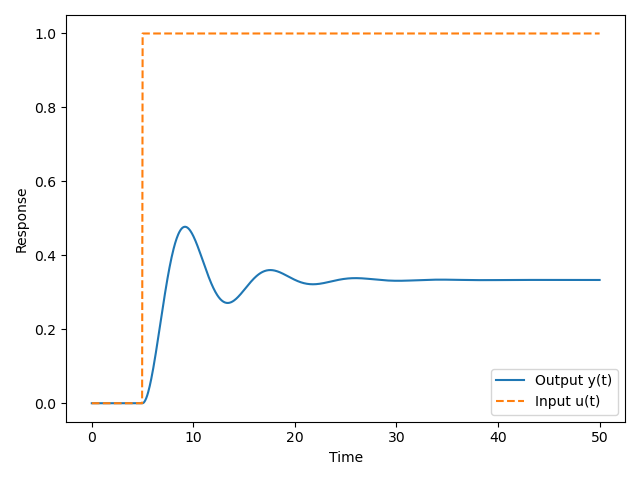
\includegraphics[scale=0.8]{../figures/mass-spring-damper-response.png}
\end{center}

Notiamo che allo stato di regime si avrà $x'' = x' = 0$ (assunta $x$ la posizione del carrello).
In questo caso la differenziale si ridurrà a:
$$
Kx = F \implies x = \frac{F}{K}
$$
che con i dati forniti dà $\sim 0.33 \, \mathrm{m}$, che come notiamo dalla figura è esattamente il punto attorno a cui il sistema si stabilizza.

\subsection{Dipendenza dalle derivate della variabile di ingresso}
Abbiamo posto finora $p = 0$, quindi nessuna derivata della variabili di ingresso.
Vediamo il caso in cui includiamo tali derivate.

\subsubsection{Caso $\mathbf{p < n}$}
Vediamo innanzitutto il caso in cui il termine di grado massimo delle variabili di stato dipende dalle derivate della variabile di ingresso, cioè $0 < p < n$.
Avevamo l'equazione differenziale:
$$
y^{(n)} (t) = \sum_{i=0}^{n-1} - \alpha_i y^{(i)}(t) + \sum_{j=0}^p \beta_j u^{(j)}(t)
$$

In questo caso la situazione si complica, e ci conviene sfruttare il \textbf{principio di sovrapposizione}.
Definiamo l'equazione ausiliaria in $z$:
$$
z^{(n)}(t) = \sum_{i = 0}^{n - 1} -\alpha_i z^{(i)}(t) + u(t)
$$
che rappresenta la risposta del sistema al solo ingresso $u(t)$ (senza derivate superiori).
Vediamo che questa è la forma che siamo stati abituati a risolvere finora.

Sarà quindi vero che la \textit{funzione forzante} (l'ingresso non scalato e non derivato) $u(t)$ porterà alla \textit{soluzione particolare} $z(t)$, cosa che indichiamo come:
$$
\mathcal{H}[u(t)] = z(t) 
$$

Considerando la linearità del sistema, siamo liberi di moltiplicare e derivare per ricavare le risposte alle funzioni derivate successive dell'ingresso scalate per i $\beta_i$ che avevamo nell'equazione originale:
\[
	\begin{cases}
		\mathcal{H}[\beta_0 u(t)] = \beta_0 z(t) \\ 
		\mathcal{H}[\beta_1 u'(t)] = \beta_1 z'(t) \\ 
		... \\
		\mathcal{H}[\beta_p u^{(p)}(t)] = \beta_p z^{(p)}(t)
	\end{cases}
\]

Per ottenere la risposta complessiva del sistema, allora, basterà applicare nuovamente la linearità e prendere la combinazione lineare delle risposte ai singoli ingressi:
$$
y(t) = \sum_{j = 0}^{p} \beta_j z^{(j)}(t)
$$
da cui il sistema finale:
\[
	\begin{cases}	
x' = \left(\begin{array}{@{}c | cccc@{}}
	0 & 1 & 0 & ... & 0 \\
	0 & 0 & 1 & ... & 0 \\
	... & ... & ... & ... & ... \\
	0 & 0 & 0 & ... & 1 \\
	\hline
	-\alpha_0 & ... & ... & ... & -\alpha_{n - 1}
\end{array}\right)
x + \begin{pmatrix}
0 \\
... \\
0 \\
1
\end{pmatrix} u \\ 
y = \begin{pmatrix}
	\beta_0 & ... & \beta_p & 0 & ... & 0
\end{pmatrix} x + \begin{pmatrix}
0
\end{pmatrix} u
	\end{cases}
\]

\subsubsection{Esempio: differenziale con derivata prima dell'ingresso}
Applichiamo il metodo appena visto per l'equazione differenziale:
$$
y'' + y = 2u + u'
$$
Notiamo il termine di derivata prima dell'ingresso $u$.
Riportandoci nella forma $y^{(n)}(t) = \hat{F}$ avremo:
$$
y'' = - y + 2u + u'
$$
con la formula al primo grado:
$$
y'' = -y + u
$$
da cui il sistema:
\[
	\begin{cases}
		\begin{pmatrix}
			x_1' \\ x_2'
		\end{pmatrix}
		=
		\begin{pmatrix}
			0 & 1 \\ 
			-1 & 0
		\end{pmatrix}
		\begin{pmatrix}
			x_1 \\ x_2
		\end{pmatrix}
		+
		\begin{pmatrix}
		0 \\ 1
		\end{pmatrix}
		u \\ 

		y = 
		\begin{pmatrix}
			2 & 1
		\end{pmatrix}
		\begin{pmatrix}
			x_1 \\ x_2
		\end{pmatrix}
		+
		\begin{pmatrix}
			0
		\end{pmatrix}
		u
	\end{cases}
\]
che sappiamo poter calcolare usando la formula di Lagrange.
In seguito vedremo un esempio di calcolo esplicito (esempio 5.0.3) per una certa configurazione di ingressi e stato iniziale.

\subsubsection{Caso $\mathbf{p = n}$}
Vediamo quindi il caso $p = n$. 
Qui avremo l'equazione differenziale:
$$
y^{(n)} (t) = \sum_{i=0}^{n-1} - \alpha_i y^{(i)}(t) + \sum_{j=0}^n \beta_j u^{(j)}(t)
$$
e la dimensione di $C$ non sarà abbastanza da contenere tutti i termini $\beta_i$.
Potremo allora definire la stessa equazione ausiliaria di prima:
$$
z^{(n)}(t) = \sum_{i = 0}^{n - 1} -\alpha_i z^{(i)}(t) + u(t)
$$
e sostituire, dopo aver preventivamente separato l'$n$-esimo termine:
$$
y(t) = \sum_{i = 1}^n \beta_{i - 1} x_i + \beta^n z^{(n)} = \sum_{i = 1}^n \beta_{i - 1} x_i + \beta_n \sum_{i = 1}^{n} -\alpha_{i - 1} z^{(i)}(t) + \beta_n u(t)
$$
da cui:
\[
	\begin{cases}	
x' = \left(\begin{array}{@{}c | cccc@{}}
	0 & 1 & 0 & ... & 0 \\
	0 & 0 & 1 & ... & 0 \\
	... & ... & ... & ... & ... \\
	0 & 0 & 0 & ... & 1 \\
	\hline
	-\alpha_0 & ... & ... & ... & -\alpha_{n - 1}
\end{array}\right)
x + \begin{pmatrix}
0 \\
... \\
0 \\
1
\end{pmatrix} u \\ 
y = \begin{pmatrix}
	\beta_0 - \beta_n \alpha_0 & ... & \beta_{n - 1} - \beta_n \alpha_{n - 1}	
\end{pmatrix} x + \begin{pmatrix}
\beta_n
\end{pmatrix} u
	\end{cases}
\]

\subsection{Rappresentazioni equivalenti}
Vediamo che la scelta di variabili di stato non è unica.
Potremmo infatti avere:
\[
	\begin{cases}
		x' = Ax + Bu \\
		y = Cx + Du
	\end{cases}
\]
e definire una matrice $T \in \mathbb{R}^{n \times n}$ invertibile detta \textbf{matrice del cambio di base} tale che:
$$
\hat{x} = Tx \implies 
\begin{cases}
	\hat{x}' = \hat{A}\hat{x} + \hat{B}u \\
	\hat{y} = \hat{C}\hat{x} + \hat{D}u
\end{cases}
$$

Ricaviamo le matrici $\hat{A}$, $\hat{B}$, $\hat{C}$ e $\hat{D}$ come:
$$
\hat{A} = T A T^{-1}, \quad \hat{B} = TB, \quad \hat{C} = CT^{-1}, \quad \hat{D} = D
$$
visto che:
\[
	\begin{cases}
		T x = T A T^{-1} T x + T B u \\ 
		y = C T^{-1} T x + D u
	\end{cases}
\]
per cancellazione di $T^{-1} T$.

Meccanicamente, questo non significa altro che possiamo prendere diversi sistemi riferimento per velocità e posizione e conservare comunque l'informazione del sistema.

\subsection{Autovalori e modi}
Avevamo dalla formula di Lagrange che per la risposta libera, cioè la soluzione di $x_l' = Ax_l$, è:
$$
	x_l(t) = e^{A(t / t_0)}x_l(t_0)
$$
posta una condizione iniziale a $t = t_0$.

Esistono 2 casi:
\begin{itemize}
	\item A \textit{diagonalizzabile};
	\item A \textit{non diagonalizzabile}.
\end{itemize}

Vediamo questi casi nel dettaglio.

\subsubsection{A diagonalizzabile}
Potremo ricavare una matrice di cambio di base $T$ tale che $A$ risulti diagonale, cioè:
$$
A = T^{-1} A_D T, \quad A_D = \begin{pmatrix}
	\lambda_1 & 0 & 0 \\
	0 & ... & 0 \\
	0 & 0 & \lambda_n
\end{pmatrix}
$$
con $A_D$ detta \textbf{matrice degli autovettori}, dove le entrate delle diagonali sono gli autovalori $A$.

In questo caso possiamo riscrivere lo stato sfruttando la serie di Taylor:
$$
\hat{x_l}(t) = e^{A_Dt} \hat{x_l}_0 = \sum_{k = 0}^\infty \frac{(A_D t)^k}{k!}\hat{x_l}_0
$$
dove la forma diagonale di $A_D$ ci permette di calcolare velocemente $A_D^k$:
$$
A_D^k = \begin{pmatrix}
	\lambda_1^k & 0 & 0 \\
	0 & ... & 0 \\
	0 & 0 & \lambda_n^k
\end{pmatrix}
$$
da cui:
$$
\hat{x_l}(t) = \mathrm{diag} \left\{ \sum_{k = 0}^\infty \frac{(\lambda_1 t)^k}{k!}, ... , \sum_{k = 0}^\infty \frac{(\lambda_n t)^k}{k!} \right\} \hat{x_l}_0
= \mathrm{diag} \left\{ e^{\lambda_1 t}, ..., e^{\lambda_n t} \right\} \hat{x_l}_0
$$
riportandoci nelle coordinate originali avremo:
$$
x_l(t) = T^{-1} \hat{x}(t) = T^{-1} \mathrm{diag} \left\{ e^{\lambda_1 t}, ..., e^{\lambda_n t} \right\} \hat{x_l}_0 = T^{-1} \mathrm{diag} \left\{ e^{\lambda_1 t}, ..., e^{\lambda_n t} \right\} T x_l(t_0)
$$

Chiamiamo gli $e^{\lambda_i}$ \textbf{modi} del sistema.
La funzioni di uscita in assenza di derivate dell'ingresso sarà quindi data da una combinazione lineare dei \textit{modi propri} del sistema:
$$
y_l(t) = C T^{-1} \mathrm{diag} \left\{ e^{\lambda_1 t}, ..., e^{\lambda_n t} \right\} T x_l(t_0)
$$

Notiamo che, come avevamo già osservato, sarà vero che $\lambda = \sigma + i \omega \in \mathbb{C}$, e quindi:
$$
e^{\lambda t} = e^{\sigma t} \cos(\omega t + \phi)
$$
dalla formula di Eulero.

\par\smallskip

Notiamo che i modi di un sistema rappresentano vari "comportamenti" naturali del sistema, che possono essere esponenziali, oscillatori o una loro combinazione sulla base del autovalore corrispondente $\lambda_i$.

Il comportamento complessivo del sistema sarà quindi dato da una qualche combinazione lineare di questi modi.

\subsubsection{A non diagonalizzabile}
Nel caso $A$ non sia diagonalizzabile si può comunque trasformare nella cosiddetta forma di \textbf{Jordan}.
Questa avrà una struttura quasi diagonale, con entrate di valore 1 immediatamente sopra la diagonale. 

In questo caso i modi assumeranno la forma:
$$
t^{\eta - 1}e^{\lambda_i} t
$$
dove $t^{\eta - 1}$ sarà un'intero compreso tra $1$ e la massima dimensione dei \textit{miniblocchi di Jordan} associati all'autovalore.

\end{document}


\documentclass[a4paper,11pt]{article}
\usepackage[a4paper, margin=8em]{geometry}

% usa i pacchetti per la scrittura in italiano
\usepackage[french,italian]{babel}
\usepackage[T1]{fontenc}
\usepackage[utf8]{inputenc}
\frenchspacing 

% usa i pacchetti per la formattazione matematica
\usepackage{amsmath, amssymb, amsthm, amsfonts}

% usa altri pacchetti
\usepackage{gensymb}
\usepackage{hyperref}
\usepackage{standalone}

% imposta il titolo
\title{Appunti Fondamenti di Automatica}
\author{Luca Seggiani}
\date{2025}

% disegni
\usepackage{pgfplots}
\pgfplotsset{width=10cm,compat=1.9}

% imposta lo stile
% usa helvetica
\usepackage[scaled]{helvet}
% usa palatino
\usepackage{palatino}
% usa un font monospazio guardabile
\usepackage{lmodern}

% tikz in sans
\tikzset{every picture/.style={/utils/exec={\sffamily}}}

\renewcommand{\rmdefault}{ppl}
\renewcommand{\sfdefault}{phv}
\renewcommand{\ttdefault}{lmtt}

% circuiti
\usepackage{circuitikz}
\usetikzlibrary{babel}

% disponi il titolo
\makeatletter
\renewcommand{\maketitle} {
	\begin{center} 
		\begin{minipage}[t]{.8\textwidth}
			\textsf{\huge\bfseries \@title} 
		\end{minipage}%
		\begin{minipage}[t]{.2\textwidth}
			\raggedleft \vspace{-1.65em}
			\textsf{\small \@author} \vfill
			\textsf{\small \@date}
		\end{minipage}
		\par
	\end{center}

	\thispagestyle{empty}
	\pagestyle{fancy}
}
\makeatother

% disponi teoremi
\usepackage{tcolorbox}
\newtcolorbox[auto counter, number within=section]{theorem}[2][]{%
	colback=blue!10, 
	colframe=blue!40!black, 
	sharp corners=northwest,
	fonttitle=\sffamily\bfseries, 
	title=Teorema~\thetcbcounter: #2, 
	#1
}

% disponi definizioni
\newtcolorbox[auto counter, number within=section]{definition}[2][]{%
	colback=red!10,
	colframe=red!40!black,
	sharp corners=northwest,
	fonttitle=\sffamily\bfseries,
	title=Definizione~\thetcbcounter: #2,
	#1
}

% disponi problemi
\newtcolorbox[auto counter, number within=section]{problem}[2][]{%
	colback=green!10,
	colframe=green!40!black,
	sharp corners=northwest,
	fonttitle=\sffamily\bfseries,
	title=Problema~\thetcbcounter: #2,
	#1
}

% disponi codice
\usepackage{listings}
\usepackage[table]{xcolor}

\lstdefinestyle{codestyle}{
		backgroundcolor=\color{black!5}, 
		commentstyle=\color{codegreen},
		keywordstyle=\bfseries\color{magenta},
		numberstyle=\sffamily\tiny\color{black!60},
		stringstyle=\color{green!50!black},
		basicstyle=\ttfamily\footnotesize,
		breakatwhitespace=false,         
		breaklines=true,                 
		captionpos=b,                    
		keepspaces=true,                 
		numbers=left,                    
		numbersep=5pt,                  
		showspaces=false,                
		showstringspaces=false,
		showtabs=false,                  
		tabsize=2
}

\lstdefinestyle{shellstyle}{
		backgroundcolor=\color{black!5}, 
		basicstyle=\ttfamily\footnotesize\color{black}, 
		commentstyle=\color{black}, 
		keywordstyle=\color{black},
		numberstyle=\color{black!5},
		stringstyle=\color{black}, 
		showspaces=false,
		showstringspaces=false, 
		showtabs=false, 
		tabsize=2, 
		numbers=none, 
		breaklines=true
}

\lstdefinelanguage{javascript}{
	keywords={typeof, new, true, false, catch, function, return, null, catch, switch, var, if, in, while, do, else, case, break},
	keywordstyle=\color{blue}\bfseries,
	ndkeywords={class, export, boolean, throw, implements, import, this},
	ndkeywordstyle=\color{darkgray}\bfseries,
	identifierstyle=\color{black},
	sensitive=false,
	comment=[l]{//},
	morecomment=[s]{/*}{*/},
	commentstyle=\color{purple}\ttfamily,
	stringstyle=\color{red}\ttfamily,
	morestring=[b]',
	morestring=[b]"
}

% disponi sezioni
\usepackage{titlesec}

\titleformat{\section}
	{\sffamily\Large\bfseries} 
	{\thesection}{1em}{} 
\titleformat{\subsection}
	{\sffamily\large\bfseries}   
	{\thesubsection}{1em}{} 
\titleformat{\subsubsection}
	{\sffamily\normalsize\bfseries} 
	{\thesubsubsection}{1em}{}

% disponi alberi
\usepackage{forest}

\forestset{
	rectstyle/.style={
		for tree={rectangle,draw,font=\large\sffamily}
	},
	roundstyle/.style={
		for tree={circle,draw,font=\large}
	}
}

% disponi algoritmi
\usepackage{algorithm}
\usepackage{algorithmic}
\makeatletter
\renewcommand{\ALG@name}{Algoritmo}
\makeatother

% disponi numeri di pagina
\usepackage{fancyhdr}
\fancyhf{} 
\fancyfoot[L]{\sffamily{\thepage}}

\makeatletter
\fancyhead[L]{\raisebox{1ex}[0pt][0pt]{\sffamily{\@title \ \@date}}} 
\fancyhead[R]{\raisebox{1ex}[0pt][0pt]{\sffamily{\@author}}}
\makeatother

\begin{document}

% sezione (data)
\section{Lezione del 05-03-25}

% stili pagina
\thispagestyle{empty}
\pagestyle{fancy}

% testo
Avevamo visto la forma standard per sistemi lineari:
\[
	\begin{cases}
		x' = Ax + Bx \\
		y = Cx + Du \\
		x(0) = x_0
	\end{cases}
\]
(con $D$ solitamente nulla), e la soluzione data da:
\[
	\begin{cases}
		x(t) = e^{At} x_0 + \int_0^t e^{A(t - \tau)} Bu(\tau) d\tau \\
		y(t) = Ce^{At} x_0 + C\int_0^t e^{A(t - \tau)} Bu(\tau) d\tau + Du \\
	\end{cases}
\]

per il calcolo di tale soluzione sfruttavamo l'\textit{esponenziale di matrice:}
$$
e^{At} = I + At + \frac{1}{2}A^2t^2+ ... + \frac{(At)^n}{n!} = \sum_{k = 0}^{+\infty} \frac{(At)^k}{k!} 
$$

Abbiamo visto che se la matrice $A$ ha autovalori distinti, allora e' diagonalizzabile:
$$
A = T^{-1} A_D T, \quad A_D = \begin{pmatrix}
	\lambda_1 & 0 & 0 \\
	0 & ... & 0 \\
	0 & 0 & \lambda_n \\
\end{pmatrix}
$$
e l'esponenziale di matrice e' semplice:
$$
e^{At} = T^{-1} e^{A_D t} T = T^{-1} \begin{pmatrix}
	e^{\lambda_1 t} & 0 & 0 \\
	0 & ... & 0 \\
	0 & 0 & e^{\lambda_n t} \\
\end{pmatrix} T
$$

In particolare, se gli autovalori sono complessi e coniugati, si avra':
$$
\lambda_i = \sigma_i + j \omega_i, \quad \overline{\lambda_i} = \sigma_i - j \omega_i 
$$
da cui:
$$
e^{\lambda_i t} = e^{\sigma_i t} e^{j\omega_i t}, \quad e^{\overline{\lambda_i} t} = e^{\sigma_i t} e^{-j\omega_i t}
$$
e si avranno quindi modi oscillatori ed esponenziali.

Avevamo inoltre definito come \textbf{modi propri} associati i:
$$
C(t) e^{\lambda t} = C(t) = \alpha_0 + \alpha_1 + \alpha_2 t^2 + ... + \alpha_{k - 1} t^{k -1}
$$

\subsubsection{Matrice reale, autovalori complessi}
Se $A$ e' reale ma i suoi autovalori sono complessi, si avra una forma del tipo:
$$
A_D = \begin{pmatrix}
	\sigma + j\omega & 0 \\
	0 & \sigma - j\omega
\end{pmatrix}
$$

Questa forma e' \textit{simile} alla matrice reale $S$:
$$
S = \begin{pmatrix}
	\sigma & \omega \\
	-\omega & \sigma
\end{pmatrix}
$$

\subsubsection{Calcolo degli autovalori}
Ripassiamo brevemente come calcolare gli autovalori.
Se $V$ e' autovettore e $\lambda$ l'autovalore associato, allora vale:
$$
Av = \lambda v \implies (A - \lambda I)v = 0 \implies \mathrm{det} (A - \lambda I) = 0
$$
detta \textbf{equazione caratteristica} $p(\lambda)$: 
$$
p(\lambda) = \mathrm{det} (A - \lambda I) = \lambda^n + \alpha_1 \lambda^{n - 1} + \alpha_2 \lambda^{n - 2} + ... + \alpha_{n - 1} \lambda + \alpha_n
$$

Avremo quindi che le soluzioni di $\lambda^*$ di $p(\lambda) = 0$ rappresentano gli autovalori di $A$.

\subsection{Forma di Jordan}
Se gli autovalori sono multipli ma $A$ non e' diagonalizzabile, abbiamo visto, occore sfruttare la \textbf{forma di Jordan} attraverso la trasformazione:
$$
J = Q A Q{-1}
$$
dove $Q$ e' la matrice degli \textbf{autovettori generalizzati} con:
$$
J = \begin{pmatrix}
	J_1 & 0 & 0 \\
	0 & ... & 0 \\
	0 & 0 & J_N
\end{pmatrix}
$$
dove ogni $J_i$ e' detto \textbf{miniblocco di Jordan}:
$$
J_i = \begin{pmatrix}
	\lambda_h & 1 & 0 & ... & 0 \\ 
	0 & \lambda_h & 1 & ... & 0 \\ 
	... & ... & ... & ... & ... \\ 
	0 & 0 & ... & \lambda_h & 1 \\
	0 & 0 & ... & 0 & \lambda_h
\end{pmatrix}
$$

Ogni blocco di Jordan ha sulla diagonale lo stesso autovalore, che compare tante volte quanto e' la sua \textit{molteplicita' algebrica}.
Inoltre, ci sono tanti blocchi $J_i$ associati allo stesso autovattore tante volte quanto e' la sua \textit{molteplicita' geometrica}.

\par\smallskip

Se riprendiamo la matrice esponenziale abbiamo:
$$
e^{At} = e^{QJQ^{-1}t} = Q \left( I + Jt + \frac{J^2 t^2}{2!} + ... + \frac{(Jt)^n}{n!} \right) Q^{-1} = Q e^{Jt} Q^{-1}
$$
dove $e^{Jt}$ e' \textit{diagonale a blocchi}:
$$
e^{Jt} = \begin{pmatrix}
e^{J_1 t} & 0 & ... & 0 \\
0 & e^{J_2 t} & ... & 0 \\
... & ... & ... & ... \\ 
0 & ... & 0 ... & e^{J_n t}
\end{pmatrix}
$$
dove ogni blocco $e^{J_i t}$ ha la forma:
$$
e^{J_i t} = e^{ \begin{pmatrix}
		\lambda & 1 & 0 \\
		0 & ... & 1 \\ 
		0 & 0 & \lambda
\end{pmatrix} t}
= e^{(\lambda I + J_{0i})t} = e^{\lambda t} e^{J_{0i} t}
$$
dove con $J_{0i}$ ci riferiamo alla \textbf{parte nilpotente} di $J_i$.
Il problema sara' quindi capire la forma di $e^{J_{0i} t}$:
$$
e^{J_{0i} t} = I + J_{0i}t + \frac{J_{0i}^2}{2!} + ... + \frac{J_{0i}^{q - i} t^{q - 1}}{(q - 1)!}
$$
dove ogni coefficiente moltiplicativo di $t^i$ ha la proprieta' di avere le entrate spostate in diagonale, verso l'alto a destra, per cui:
$$
e^{J_{0i} t} = \begin{pmatrix}
	1 & t & \frac{t^2}{2} & ... & \frac{t^{(q - 1)}}{(q - 1)!} \\
	0 & 1 & t & ... & ... \\
	0 & 0 & 1 & t & \frac{t^2}{2} \\ 
	0 & 0 & 0 & 1 & t \\
	0 & 0 & 0 & 0 & 1
\end{pmatrix}
$$
e quindi i modi del sistema sarano:
$$
t^k \frac{e^{\lambda t}}{k!}, \quad 0 \leq k \leq q - 1
$$
dove abbiamo finalmente capito il significato dell'intero $k$.

\par\smallskip
Notiamo che la proprieta' di similarita' che avevamo trovato:
$$
M = \begin{pmatrix}
	\sigma + j\omega & 0 \\
	0 & \sigma - j\omega
\end{pmatrix}
\sim
S = \begin{pmatrix}
	\sigma & \omega \\
	-\omega & \sigma
\end{pmatrix}
$$
ha un equivalente per le matrici in forma di Jordan:
$$
M=
\begin{pmatrix}
	\sigma + j \omega & 1 & 0 & 0 \\
	0 & \sigma + j \omega & 0 & 0 \\
	0 & 0 & \sigma - j \omega & 1 \\
	0 & 0 & 0 & \sigma - j \omega
\end{pmatrix}
\sim 
S=
\begin{pmatrix}
	\sigma & \omega & 1 & 0 \\
	-\omega & \sigma & 0 & 1 \\
	0 & 0 & \sigma & \omega \\
	0 & 0 & -\omega & \sigma \\
\end{pmatrix}
$$

e via dicendo.

\subsection{Stabilit' nei sistemi lineari stazionari}
Riprendiamo la definizione di \textit{stabilita'} (3.3 e 3.4).
Quello che interessa sono le \textbf{perturbazioni} dello stato.

Per un sistema lineare e stazionario l'origine e' sempre punto di equilibrio per ingresso nullo.
Se l'origine e' stabile, allora lo e' qualsiasi altro punto di equilibrio.
Si puo' allore dire che un sistema e' \textbf{stabile} solo guardando alla risposta \textit{libera} del sistema:
$$
x' = Ax + Bu, \quad u = 0, \quad x(0) = x_0
$$
$$
x(t) = e^{At}x_0
$$

In particolare, la stabilita' del sistema dipende dai \textit{modi propri} del sistema.
In particolare, se gli autovalori hanno parte reale $\mathrm{Re}(\lambda_i) < 0$ il sistema e' \textbf{asintoticamente stabile}, mentre se hanno parte reale $\mathrm{Re}(\lambda_i) \leq 0$ e gli $\mathrm{Re}(\lambda_i) = 0$ hanno molteplicita' $\mu =1$ il sistema e' solo \textbf{stabile}.
Quest'ultimo caso e' propriamente quello delle matrici non diagonalizzabili (quindi messe in forma di Jordan).

Possiamo riassumere la relazione fra stabilita', modi e autovalori come segue:
\begin{table}[H]
	\center \rowcolors{2}{white}{black!10}
	\begin{tabular} { p{3.5cm} | p{5cm} | p{5cm} }
		\bfseries Stabilita' & \bfseries Modi & \bfseries Autovalori \\
		\hline
		Stabilita' asintotica & Tendono a zero & $\mathrm{Re}(\lambda_i) < 0$ \\
	Stabilita' semplice o marginale & Non vanno a infinito, ma almeno uno non converge a zero & $\mathrm{Re}(\lambda_i) \leq 0$, $\exists \lambda_i^* : \mathrm{Re}(\lambda_i^*) = 0$, $\mu = 1$ \\
Instabilita' & Almeno uno va a infinito & $\mathrm{Re}(\lambda_i) > 0$ o $\exists \lambda_i^* : \mathrm{Re}(\lambda_i^*)$, $\mu_a(\lambda_i^*) \neq \mu_g(\lambda_i^*)$ \\
	\end{tabular}
\end{table}

\subsubsection{Stabilita' dei sistemi linearizzati}
Avevamo visto che nei sistemi non lineari conviene \textit{linearizzare} trascurando i termini oltre il primo ordine nell'intorno di uno stato di equilibrio noto.
Se il sistema linearizzato e' \textit{asintoticamente stabile}, si avra' che lo stato di equilibrio del sistema non lineare e' \textbf{stabile}.
Di contro, se il sistema linearizzato e' \textit{semplicemente stabile} non possiamo concludere nulla sul sistema non lineare (potrebbero esserci instabilita' ai termini superiori).

\end{document}


\documentclass[a4paper,11pt]{article}
\usepackage[a4paper, margin=8em]{geometry}

% usa i pacchetti per la scrittura in italiano
\usepackage[french,italian]{babel}
\usepackage[T1]{fontenc}
\usepackage[utf8]{inputenc}
\frenchspacing 

% usa i pacchetti per la formattazione matematica
\usepackage{amsmath, amssymb, amsthm, amsfonts}

% usa altri pacchetti
\usepackage{gensymb}
\usepackage{hyperref}
\usepackage{standalone}

% imposta il titolo
\title{Appunti Fondamenti di Automatica}
\author{Luca Seggiani}
\date{2025}

% disegni
\usepackage{pgfplots}
\pgfplotsset{width=10cm,compat=1.9}

% imposta lo stile
% usa helvetica
\usepackage[scaled]{helvet}
% usa palatino
\usepackage{palatino}
% usa un font monospazio guardabile
\usepackage{lmodern}

% tikz in sans
\tikzset{every picture/.style={/utils/exec={\sffamily}}}

\renewcommand{\rmdefault}{ppl}
\renewcommand{\sfdefault}{phv}
\renewcommand{\ttdefault}{lmtt}

% circuiti
\usepackage{circuitikz}
\usetikzlibrary{babel}

% disponi il titolo
\makeatletter
\renewcommand{\maketitle} {
	\begin{center} 
		\begin{minipage}[t]{.8\textwidth}
			\textsf{\huge\bfseries \@title} 
		\end{minipage}%
		\begin{minipage}[t]{.2\textwidth}
			\raggedleft \vspace{-1.65em}
			\textsf{\small \@author} \vfill
			\textsf{\small \@date}
		\end{minipage}
		\par
	\end{center}

	\thispagestyle{empty}
	\pagestyle{fancy}
}
\makeatother

% disponi teoremi
\usepackage{tcolorbox}
\newtcolorbox[auto counter, number within=section]{theorem}[2][]{%
	colback=blue!10, 
	colframe=blue!40!black, 
	sharp corners=northwest,
	fonttitle=\sffamily\bfseries, 
	title=Teorema~\thetcbcounter: #2, 
	#1
}

% disponi definizioni
\newtcolorbox[auto counter, number within=section]{definition}[2][]{%
	colback=red!10,
	colframe=red!40!black,
	sharp corners=northwest,
	fonttitle=\sffamily\bfseries,
	title=Definizione~\thetcbcounter: #2,
	#1
}

% disponi problemi
\newtcolorbox[auto counter, number within=section]{problem}[2][]{%
	colback=green!10,
	colframe=green!40!black,
	sharp corners=northwest,
	fonttitle=\sffamily\bfseries,
	title=Problema~\thetcbcounter: #2,
	#1
}

% disponi codice
\usepackage{listings}
\usepackage[table]{xcolor}

\lstdefinestyle{codestyle}{
		backgroundcolor=\color{black!5}, 
		commentstyle=\color{codegreen},
		keywordstyle=\bfseries\color{magenta},
		numberstyle=\sffamily\tiny\color{black!60},
		stringstyle=\color{green!50!black},
		basicstyle=\ttfamily\footnotesize,
		breakatwhitespace=false,         
		breaklines=true,                 
		captionpos=b,                    
		keepspaces=true,                 
		numbers=left,                    
		numbersep=5pt,                  
		showspaces=false,                
		showstringspaces=false,
		showtabs=false,                  
		tabsize=2
}

\lstdefinestyle{shellstyle}{
		backgroundcolor=\color{black!5}, 
		basicstyle=\ttfamily\footnotesize\color{black}, 
		commentstyle=\color{black}, 
		keywordstyle=\color{black},
		numberstyle=\color{black!5},
		stringstyle=\color{black}, 
		showspaces=false,
		showstringspaces=false, 
		showtabs=false, 
		tabsize=2, 
		numbers=none, 
		breaklines=true
}

\lstdefinelanguage{javascript}{
	keywords={typeof, new, true, false, catch, function, return, null, catch, switch, var, if, in, while, do, else, case, break},
	keywordstyle=\color{blue}\bfseries,
	ndkeywords={class, export, boolean, throw, implements, import, this},
	ndkeywordstyle=\color{darkgray}\bfseries,
	identifierstyle=\color{black},
	sensitive=false,
	comment=[l]{//},
	morecomment=[s]{/*}{*/},
	commentstyle=\color{purple}\ttfamily,
	stringstyle=\color{red}\ttfamily,
	morestring=[b]',
	morestring=[b]"
}

% disponi sezioni
\usepackage{titlesec}

\titleformat{\section}
	{\sffamily\Large\bfseries} 
	{\thesection}{1em}{} 
\titleformat{\subsection}
	{\sffamily\large\bfseries}   
	{\thesubsection}{1em}{} 
\titleformat{\subsubsection}
	{\sffamily\normalsize\bfseries} 
	{\thesubsubsection}{1em}{}

% disponi alberi
\usepackage{forest}

\forestset{
	rectstyle/.style={
		for tree={rectangle,draw,font=\large\sffamily}
	},
	roundstyle/.style={
		for tree={circle,draw,font=\large}
	}
}

% disponi algoritmi
\usepackage{algorithm}
\usepackage{algorithmic}
\makeatletter
\renewcommand{\ALG@name}{Algoritmo}
\makeatother

% disponi numeri di pagina
\usepackage{fancyhdr}
\fancyhf{} 
\fancyfoot[L]{\sffamily{\thepage}}

\makeatletter
\fancyhead[L]{\raisebox{1ex}[0pt][0pt]{\sffamily{\@title \ \@date}}} 
\fancyhead[R]{\raisebox{1ex}[0pt][0pt]{\sffamily{\@author}}}
\makeatother

\begin{document}

% sezione (data)
\section{Lezione del 06-03-25}

% stili pagina
\thispagestyle{empty}
\pagestyle{fancy}

% testo
\subsection{Forma di Jordan con autovalori complessi e coniugati}
Nel caso si trovi $A$ matrice reale con autovalori complessi e coniugati, è possibile usare un cambio di coordinate che trasforma la matrice diagonale complessa in una matrice reale diagonale a blocchi.

Questo è il caso che abbiamo già visto di:
$$
\begin{pmatrix}
	\sigma & \omega \\
	-\omega & \sigma
\end{pmatrix}
\sim
\begin{pmatrix}
	\sigma + j\omega & 0 \\
	0 & \sigma - j \omega
\end{pmatrix}
$$
e:
$$
\begin{pmatrix}
	\sigma & \omega & 1 & 0 \\
	-\omega & \sigma & 0 & 1 \\
	0 & 0 & \sigma & \omega \\
	0 & 0 & -\omega & \sigma \\
\end{pmatrix}
\sim
\begin{pmatrix}
	\sigma + j \omega & 1 & 0 & 0 \\
	0 & \sigma + j \omega & 0 & 0 \\
	0 & 0 & \sigma - j \omega & 1 \\
	0 & 0 & 0 & \sigma - j \omega
\end{pmatrix} 
$$

In generale, quindi, abbiamo matrici di Jordan:
$$
J_r = \begin{pmatrix}
	M & I & 0 & ... & 0 \\
	0 & M & I & ... & 0 \\
	0 & ... & M & I & 0 \\ 
	0 & ... &  0 & M & I \\
	0 & ... & ... & 0 & M
\end{pmatrix}
$$
dove gli $M$ rappresentano i singoli miniblocchi:
$$
M = \begin{pmatrix}
	\sigma & \omega \\
	-\omega & \sigma
\end{pmatrix}
$$

Il numero di blocchi è quindi pari al numero di coppie di autovalori complessi coniugati.

\subsection{Raggiungibilità}
Abbiamo visto come la proprietà di stabilita dipende solo dalla struttura del sistema, e in particolare dalla sola matrice $A$.

Vediamo come in verità esistono altre proprietà che dipendono dalla struttura del sistema e che ci sono di interesse dal punto di vista della regolazione automatica.
Una di queste proprietà è la \textbf{raggiungibilità}.

Diamo quindi la definizione:
\begin{definition}{Raggiungibilità}
	Dato il sistema dinamico di ordine $n$ con $m$ ingressi e $p$ uscite:
	\[
		\begin{cases}
			x' = Ax + Bu \\
			y = Cx + Du
		\end{cases}
	\]
		allora uno stato $\overline{x}$ si dice raggiungibile se esistono un istante di tempo finito $\overline{t} > 0$ e un ingresso $\overline{u}$ definito tra $0$ e $\overline{t}$ tali che, detto $\overline{x}_f(t)$ il movimento forzato dello stato generato da $\overline{u}$, risulti che $\overline{x}_f(\overline{t}) = \overline{x}$.
\end{definition}

La proprieta di raggiungibilità degli stati divide gli stessi in due categorie: stati raggiungibili e stati non raggiungibili.

\subsubsection{Completa raggiungibilità}
Se tutti gli stati di un sistema sono raggiungibili, allora il sistema è detto \textbf{completamente raggiungibile}.

Si può verificare se un sistema è completamente raggiungible sfruttando la matrice:

$$
\mathcal{M}_\mathcal{R} = \begin{pmatrix}
	B & AB & A^B & ... & A^{n - 1}B
\end{pmatrix}
$$
e verificando se:
$$
\mathrm{rank}(\mathcal{M}_\mathcal{R}) = n
$$

Nel caso un sistema non sia completamente raggiungibile si può isolare la parte raggiungibile, cioè definire una trasformazione $T_r$ che ci porti:
$$
x' = Ax + Bu, \quad \hat{x} = T_r x \implies \hat{x}' = \hat{A} \hat{x} + \hat{B} u
$$
con:
$$
\hat{A} = \begin{pmatrix}
\hat{A}_a & \hat{A}_{ab} \\
0 & \hat{A}_b
\end{pmatrix}, \quad
\hat{B} = \begin{pmatrix}
	\hat{B}_a \\
	0
\end{pmatrix}
$$

con $\hat{A}_a \in \mathbb{R}^{n_r \times n_r}$ e $\hat{B}_a \in \mathbb{R}^{n_r \times m}$, con $n_r = \mathrm{rank}(\mathcal{M}_\mathcal{R})$.

Posto:
$$
\hat{x} = \begin{pmatrix}
	\hat{x}_r \\ 
	\hat{x}_{nr}
\end{pmatrix}
$$
si avrà svolgendo le moltiplicazioni che:
\[
	\begin{cases}
		\hat{x}_r' = \hat{A}_a \hat{x}_r + \hat{A}_{ab} \hat{x}_{nr} + \hat{B}_a u\\
		\hat{x}_{nr}' = \hat{A}_b \hat{x}_{nr}
	\end{cases}
\]
ovvero si divide lo stato in una parte raggiungibile e in una parte non raggiungibile.

\subsubsection{Ricavare la matrice $\mathbf{T_r}$}
Per ricavare la matrice di trasformazione $T_r$ basterà scegliere $n_r$ colonne linearmente indipendenti di $\mathcal{M}_\mathcal{R}$.
Ogni stato raggiungibile sarà combinazione lineare di queste colonne.
Si aggiungono poi $n - n_r$ colonne linearmente indipendenti, prese ad arbitrio.

\end{document}


\documentclass[a4paper,11pt]{article}
\usepackage[a4paper, margin=8em]{geometry}

% usa i pacchetti per la scrittura in italiano
\usepackage[french,italian]{babel}
\usepackage[T1]{fontenc}
\usepackage[utf8]{inputenc}
\frenchspacing 

% usa i pacchetti per la formattazione matematica
\usepackage{amsmath, amssymb, amsthm, amsfonts}

% usa altri pacchetti
\usepackage{gensymb}
\usepackage{hyperref}
\usepackage{standalone}

% imposta il titolo
\title{Appunti Fondamenti di Automatica}
\author{Luca Seggiani}
\date{2025}

% disegni
\usepackage{pgfplots}
\pgfplotsset{width=10cm,compat=1.9}

% imposta lo stile
% usa helvetica
\usepackage[scaled]{helvet}
% usa palatino
\usepackage{palatino}
% usa un font monospazio guardabile
\usepackage{lmodern}

% tikz in sans
\tikzset{every picture/.style={/utils/exec={\sffamily}}}

\renewcommand{\rmdefault}{ppl}
\renewcommand{\sfdefault}{phv}
\renewcommand{\ttdefault}{lmtt}

% circuiti
\usepackage{circuitikz}
\usetikzlibrary{babel}

% disponi il titolo
\makeatletter
\renewcommand{\maketitle} {
	\begin{center} 
		\begin{minipage}[t]{.8\textwidth}
			\textsf{\huge\bfseries \@title} 
		\end{minipage}%
		\begin{minipage}[t]{.2\textwidth}
			\raggedleft \vspace{-1.65em}
			\textsf{\small \@author} \vfill
			\textsf{\small \@date}
		\end{minipage}
		\par
	\end{center}

	\thispagestyle{empty}
	\pagestyle{fancy}
}
\makeatother

% disponi teoremi
\usepackage{tcolorbox}
\newtcolorbox[auto counter, number within=section]{theorem}[2][]{%
	colback=blue!10, 
	colframe=blue!40!black, 
	sharp corners=northwest,
	fonttitle=\sffamily\bfseries, 
	title=Teorema~\thetcbcounter: #2, 
	#1
}

% disponi definizioni
\newtcolorbox[auto counter, number within=section]{definition}[2][]{%
	colback=red!10,
	colframe=red!40!black,
	sharp corners=northwest,
	fonttitle=\sffamily\bfseries,
	title=Definizione~\thetcbcounter: #2,
	#1
}

% disponi problemi
\newtcolorbox[auto counter, number within=section]{problem}[2][]{%
	colback=green!10,
	colframe=green!40!black,
	sharp corners=northwest,
	fonttitle=\sffamily\bfseries,
	title=Problema~\thetcbcounter: #2,
	#1
}

% disponi codice
\usepackage{listings}
\usepackage[table]{xcolor}

\lstdefinestyle{codestyle}{
		backgroundcolor=\color{black!5}, 
		commentstyle=\color{codegreen},
		keywordstyle=\bfseries\color{magenta},
		numberstyle=\sffamily\tiny\color{black!60},
		stringstyle=\color{green!50!black},
		basicstyle=\ttfamily\footnotesize,
		breakatwhitespace=false,         
		breaklines=true,                 
		captionpos=b,                    
		keepspaces=true,                 
		numbers=left,                    
		numbersep=5pt,                  
		showspaces=false,                
		showstringspaces=false,
		showtabs=false,                  
		tabsize=2
}

\lstdefinestyle{shellstyle}{
		backgroundcolor=\color{black!5}, 
		basicstyle=\ttfamily\footnotesize\color{black}, 
		commentstyle=\color{black}, 
		keywordstyle=\color{black},
		numberstyle=\color{black!5},
		stringstyle=\color{black}, 
		showspaces=false,
		showstringspaces=false, 
		showtabs=false, 
		tabsize=2, 
		numbers=none, 
		breaklines=true
}

\lstdefinelanguage{javascript}{
	keywords={typeof, new, true, false, catch, function, return, null, catch, switch, var, if, in, while, do, else, case, break},
	keywordstyle=\color{blue}\bfseries,
	ndkeywords={class, export, boolean, throw, implements, import, this},
	ndkeywordstyle=\color{darkgray}\bfseries,
	identifierstyle=\color{black},
	sensitive=false,
	comment=[l]{//},
	morecomment=[s]{/*}{*/},
	commentstyle=\color{purple}\ttfamily,
	stringstyle=\color{red}\ttfamily,
	morestring=[b]',
	morestring=[b]"
}

% disponi sezioni
\usepackage{titlesec}

\titleformat{\section}
	{\sffamily\Large\bfseries} 
	{\thesection}{1em}{} 
\titleformat{\subsection}
	{\sffamily\large\bfseries}   
	{\thesubsection}{1em}{} 
\titleformat{\subsubsection}
	{\sffamily\normalsize\bfseries} 
	{\thesubsubsection}{1em}{}

% disponi alberi
\usepackage{forest}

\forestset{
	rectstyle/.style={
		for tree={rectangle,draw,font=\large\sffamily}
	},
	roundstyle/.style={
		for tree={circle,draw,font=\large}
	}
}

% disponi algoritmi
\usepackage{algorithm}
\usepackage{algorithmic}
\makeatletter
\renewcommand{\ALG@name}{Algoritmo}
\makeatother

% disponi numeri di pagina
\usepackage{fancyhdr}
\fancyhf{} 
\fancyfoot[L]{\sffamily{\thepage}}

\makeatletter
\fancyhead[L]{\raisebox{1ex}[0pt][0pt]{\sffamily{\@title \ \@date}}} 
\fancyhead[R]{\raisebox{1ex}[0pt][0pt]{\sffamily{\@author}}}
\makeatother

\begin{document}

% sezione (data)
\section{Lezione del 11-03-25}

% stili pagina
\thispagestyle{empty}
\pagestyle{fancy}

% testo
Vediamo alcuni esempi sulla raggiungibilità introdotta alla scorsa lezione.

\subsubsection{Esempio: raggiungibilità della velocità di crociera}
Riprendiamo l'esempio 3.0.1 (in particolare, la linearizzazione data in 3.1.2) e studiamone la raggiungibilità.

Avevamo che il sistema era espresso con le matrici $A, B, C, D$:
\[
	\begin{cases}
		x' = \begin{pmatrix}
			0 & 1 \\
			0 & -\frac{\beta}{m}
		\end{pmatrix} x + \begin{pmatrix}
			0 & 0 \\ 
			\frac{\gamma}{m} & -g
		\end{pmatrix}	u \\ 
		y = \begin{pmatrix}
			0 & 1
		\end{pmatrix} x
	\end{cases}
\]

Ricaviamo quindi la matrice $\mathcal{M}_\mathcal{R}$:
$$
\mathcal{M}_\mathcal{R} = \begin{pmatrix}
	B & A B
\end{pmatrix} = \begin{pmatrix}
	0 & 0 & \frac{\gamma}{m} & -g \\
	\frac{\gamma}{m} & -g & -\frac{\beta \gamma}{m^2} & \frac{g \beta}{m}
\end{pmatrix}
$$
notiamo che le due righe sono necessariamente indipendenti, ergo $\mathrm{rank}(\mathcal{M}_\mathcal{R}) = n = 2$, e il sistema è completamente raggiungibile.

\subsubsection{Esempio: raggiungibilità di una coppia di condensatori}
Vediamo quindi un sistema non completamente raggiungibile per evidenziare come ricavare le parti raggiungibili e non raggiungibili.

Prendiamo il circuito dato dalla coppia di condensatori in serie:
\begin{center}
	\begin{circuitikz}
		\draw (0, 0) to[capacitor, v<=$V_1$] (3, 0)
			to[resistor, l=$R$] (3, -3)
			to[capacitor, v<=$V_2$] (0, -3)
			to[voltage source, v=$u$] (0, 0);	
	\end{circuitikz}
\end{center}

Dal punto di vista fisico avremo che:
$$
i = C \frac{d v_1}{dt} = C \frac{d v_2}{dt}
$$
e dalla seconda di Kirchoff:
$$
u = v_1 + v_2 + i R \implies i = \frac{u - v_1 - v_2}{R}
$$
quindi:
$$
\frac{u - v_1 - v_2}{RC} = \frac{d v_1}{dt} = \frac{d v_2}{dt}
$$
da cui si ricava il sistema finale:
\[
	\begin{cases}
		\frac{d v_1}{dt} = -\frac{1}{RC} (v_1 + v_2) + \frac{1}{RC} u \\ 	
		\frac{d v_2}{dt} = -\frac{1}{RC} (v_1 + v_2) + \frac{1}{RC} u \\ 	
	\end{cases}
\]
con matrici $A$ e $B$ (la $C$ non ci è immediatamente di interesse, e dipenderà comunque dalla variabile che desideriamo osservare):
$$
A = \begin{pmatrix}
	-\frac{1}{RC} & -\frac{1}{RC} \\
	-\frac{1}{RC} & -\frac{1}{RC} \\
\end{pmatrix}, \quad B = \begin{pmatrix}
	\frac{1}{RC} \\ \frac{1}{RC}
\end{pmatrix}
$$

Possiamo quindi calcolare la matrice $\mathcal{M}_\mathcal{R}$:
$$
\mathcal{M}_\mathcal{R} = \begin{pmatrix}
	\frac{1}{RC} & -\frac{2}{R^2C^2} \\ 
	\frac{1}{RC} & -\frac{2}{R^2C^2} \\ 
\end{pmatrix}
$$
che ha chiaramente $\mathrm{rank}(\mathcal{M}_\mathcal{R}) = 1$ (righe linearmente dipendenti), cioè il sistema non è completamente raggiungibile.

In particolare, prendiamo la matrice di trasformazione $T_r$:
$$
T_r = \frac{1}{2} \begin{pmatrix}
	1 & 1 \\ 
	1 & -1
\end{pmatrix}, \quad
T_r^{-1} = \begin{pmatrix}
	-1 & -1 \\ 
	-1 & 1
\end{pmatrix}
$$

da cui la trasformazione in $\hat{A}$:
$$
\hat{A} = T_r A T_r^{-1} = \frac{1}{2} \begin{pmatrix}
	1 & 1 \\
	1 & -1
\end{pmatrix} \begin{pmatrix}
	\frac{1}{RC} & \frac{1}{RC} \\ 
	\frac{1}{RC} & \frac{1}{RC} 
\end{pmatrix}
\begin{pmatrix}
	-1 & -1 \\
	-1 & 1
\end{pmatrix} = \begin{pmatrix}
	\frac{-2}{RC} & 0 \\
	0 & 0
\end{pmatrix}
$$

Si ricava quindi il sistema:
\[
	\begin{cases}
		\hat{x}_1' = -\frac{2}{RC} (\hat{x}_1 - u) \\
		\hat{x}_2' = 0
	\end{cases}
\]

Vediamo che la variabile $x_2$ ha derivata nulla indipendentemente dall'ingresso, ergo uno stato $x_2 \neq x_2(0)$ è impossibile da raggiungere.

Notiamo infine che questa è la stessa trasformazione che avremmo potuto ottenere, ad esempio, imponendo $\hat{x}_2 = v_1 - v_2$.

\subsubsection{Conclusioni sulla raggiungibilità}
Abbiamo quindi che, per sistemi LTI, la raggiungibilità corrisponde con la controllabilità (portare il sistema da uno stato qualsiasi all'origine).
Se la parte non controllabile di un sistema è asintoticamente stabile (cioè ha parte reale degli autovalori $< 0$ il sistema si dice \textbf{stabilizzante}).
Per un sistema completamente controllabile invece esiste sempre almeno un ingresso che permette di spostarsi da uno stato $x_a$ a uno stato $x_b$.

\subsection{Osservabilità}
Vediamo quindi l'ultima proprietà strutturale dei sistemi dinamici: quella di \textbf{osservabilità}.
Questa dipenderà dalle relazioni fra stato e uscita, e quindi dalle matrici $A$ e $C$.

Diamo innanzitutto la definizione:
\begin{definition}{Osservabilità}
	Preso il sistema dinamico di ordine $n$, con $m$ ingressi e $p$ uscite:
	\[
		\begin{cases}
			x' = Ax + Bu \\ 
			y = Cx + Du
		\end{cases}
	\]
	allora uno stato $\overline{x} \neq 0$ si dice non osservabile se, qualunque sia $\overline{t} > 0$ finito, detto $\overline{y}_l(t)$ su $t \geq 0$ il movimento libero dell'uscita generato da $\overline{x}$, risulta $\overline{y}_l(t) = 0$ per $0 \leq t \leq \overline{t}$.
\end{definition}

Come vediamo, l'osservabilità ci dà un indicazione della possibilità di "vedere" la presenza di un certo stato in un certo sistema controllandone l'uscita.


\subsubsection{Completa osservabilità}
Abbiamo quindi che uno stato iniziale $x$ si dice osservabile se è possibile determinare $x$ sulla base della misura delle uscite $y$.
In particolare, un sistema privo di stati non osservabili (cioè un sistema dove tutti gli stati sono osservabili) si dice \textbf{completamente osservabile}.

Si può verificare se un sistema è completamente osservabile sfruttando la matrice (\textit{di osservabilità}):
$$
\mathcal{M}_\mathcal{O} = \begin{pmatrix}
C \\ 
C A \\
C A^2 \\
... \\
C A^{n - 1}
\end{pmatrix}
$$
e verificando se:
$$
\mathrm{rank}(\mathcal{M}_\mathcal{O}) = n
$$

Anche l'osservabilità divide gli stati in una parte osservabile e in una parte non osservabile:
$$
\hat{x} = \begin{pmatrix}
	\hat{x}_o \\ 
	\hat{x}_{no}
\end{pmatrix}
$$
sfruttando la matrice $T_o$:
$$
x' = Ax + Bu, \quad \hat{x} = T_o x \implies \hat{x}' = \hat{A} \hat{x} 
$$
$$
y = Cx, \quad \hat{x} = T_o x \implies y = \hat{C} \hat{x}
$$
con:
$$
\hat{A} = \begin{pmatrix}
	\hat{A} & 0 \\ 
	\hat{A}_{ba} & \hat{A}_b
\end{pmatrix}, \quad 
\hat{C} = \begin{pmatrix}
	\hat{C}_a & 0
\end{pmatrix}
$$
con $\hat{A}_a \in \mathbb{R}^{n_o \times n_o}$ e $\hat{C}_a \in \mathbb{R}^{p \times n_o}$, e con $n_o = \mathrm{rank}(\mathcal{M}_\mathcal{O})$, $n_o < n$.

Svolgendo le moltiplicazioni si avrà che:
\[
	\begin{cases}
		\hat{x}_{o}' = \hat{A}_a \hat{x}_{o} \\	
		\hat{x}_{no}' = \hat{A}_{ba} \hat{x}_{o} + \hat{A}_{b} \hat{x}_{no} \\
		y = \hat{C}_a \hat{x}_{no}
	\end{cases}
\]

\subsubsection{Ricavare la matrice $\mathbf{T_o}$}
Per ricavare la matrice di trasformazione $T_o$ dovremo scegliere $n - n_o$ vettori $\xi_i$ linearmente indipendenti tali che:
$$
\mathcal{M}_\mathcal{O} \xi_i = 0, \quad \mathrm{span}\left( \{ \xi_i \} \right) = x_{no}
$$
tali che compongono una base del $\mathrm{ker}(\mathcal{M}_\mathcal{O})$, ovvero ogni vettore rappresenta uno stato non osservabile.

Si selezionano poi $n_o$ vettori linearmente indipendenti ad aribtrio per completare la matrice, tali che:
$$
\det(T_o^{-1}) \neq 0
$$
cioè $T_o$ è invertibile.

\subsubsection{Esempio: osservabilità di una massa con attrito}
Prendiamo l'esempio di una massa soggetta ad attrito dipendente dalla velocità:
\[
	\begin{cases}
		x_1' = -\frac{c}{m} x_1 + \frac{1}{m} u \\ 
		x_2' = x_1 \\
		y = x_1
	\end{cases}
\]
dove prendiamo $x_1$ come velocità e $x_2$ posizione (contro ogni aspettativa, perchè qui ci piace essere imprevedibili).

Le matrici $A$ e $C$ saranno allora:
$$
A = \begin{pmatrix}
	-\frac{c}{m} & 0 \\
	1 & 0
\end{pmatrix}, \quad C = \begin{pmatrix}
	1 & 0
\end{pmatrix}
$$
e la matrice di osservabilità sarà:
$$
\mathcal{M}_\mathcal{O} = \begin{pmatrix}
	C \\ C A
\end{pmatrix} = \begin{pmatrix}
	1 & 0 \\ 
	-\frac{c}{m} & 0
\end{pmatrix}
$$
che con le righe linearmente dipendenti dà $\mathrm{rank}(\mathcal{M}_\mathcal{O}) = 1$, cioè il sistema non è completamente osservabile (questo sarebbe risultato chiaro anche guardando la definizione di $y$, dove si ha solo lo stato $x_1$ e nessuna informazione riguardo a $x_2$).

\subsubsection{Esempio: osservabilità della velocità di crociera}
Riprendiamo nuovamente l'esempio 3.0.1 (linearizzazione 3.1.2), e studiamone, stavolta, l'osservabilità.
Ricordiamo ancora che il sistema era:
\[
	\begin{cases}
		x' = \begin{pmatrix}
			0 & 1 \\
			0 & -\frac{\beta}{m}
		\end{pmatrix} x + \begin{pmatrix}
			0 & 0 \\ 
			\frac{\gamma}{m} & -g
		\end{pmatrix}	u \\ 
		y = \begin{pmatrix}
			0 & 1
		\end{pmatrix} x
	\end{cases}
\]

Ricaviamo quindi la matrice $\mathcal{M}_\mathcal{O}$:
$$
\mathcal{M}_\mathcal{O} = \begin{pmatrix}
 C \\ C A
\end{pmatrix} = \begin{pmatrix}
	0 & 1 \\
	0 & -\frac{\beta}{m}
\end{pmatrix}
$$

Vediamo subbito che le due righe della matrice sono linearmente dipendenti, ergo $\mathrm{rank}(\mathcal{M}_\mathcal{O}) = 1$ e il sistema non è completamente osservabile.
Nel caso particolare dell'automobile, avremo che sarà impossibile ricostruire la posizione iniziale conoscendo solo la velocità.

\subsection{Scomposizione canonica}
Un sistema può essere sia non completamente osservabile che non completamente raggiungibile.
Esiste una scomposizione che porta il sistema in una forma che ne evidenzia tutte queste caratteristiche, detta \textbf{forma canonica} (\textit{forma canonica di Kalman}), solitamente indicata con $T_k$.

Vogliamo quindi la trasformazione:
$$
\hat{x} = T_k x \rightarrow
\begin{cases}
	\hat{x}' = \hat{A} \hat{x} + \hat{B} u \\
	y = \hat{C} \hat{x} + \hat{D} u
\end{cases}
$$
che prende la forma:
\[
	\begin{cases}			
\hat{x}' = \begin{pmatrix}
	\hat{A}_a & \hat{A}_{ab} & \hat{A}_{ac} & \hat{A}_{ad} & \\
	0 & \hat{A}_b & 0 & \hat{A}_{bd} & \\
	0 & 0 & \hat{A}_c & \hat{A}_{cd} \\ 
	0 & 0 & 0 & \hat{A}_d
\end{pmatrix} \hat{x} + \begin{pmatrix}
	\hat{B}_a \\ \hat{B}_b \\ 0 \\ 0
\end{pmatrix} u \\
y = \begin{pmatrix}
	0 & \hat{C}_b & 0 & \hat{C}_d
\end{pmatrix} \hat{x}
	\end{cases}
\]
con:
$$
\hat{x} = \begin{pmatrix}
	\hat{x}_a \\ 
	\hat{x}_b \\ 
	\hat{x}_c \\ 
	\hat{x}_d \\ 
\end{pmatrix}
$$
dove:
\begin{itemize}
	\item $\hat{x}_a$ rappresenta la parte \textbf{raggiungibile non osservabile}; 
	\item $\hat{x}_b$ rappresenta la parte \textbf{non raggiungibile non osservabile}; 
	\item $\hat{x}_c$ rappresenta la parte \textbf{raggiungibile non osservabile}; 
	\item $\hat{x}_d$ rappresenta la parte \textbf{non raggiungibile osservabile}; 
\end{itemize}

Notiamo che gli autovalori della matrice triangolare a blocchi $A$ sono gli stessi della matrice $A$ originale (li ricaviamo dalla diagonale $\hat{A}_a, \hat{A}_b, \hat{A}_c, \hat{A}_d,$), ergo queste sono simili, anche se siamo riusciti ad isolare ogni parte di interesse.

\end{document}


\documentclass[a4paper,11pt]{article}
\usepackage[a4paper, margin=8em]{geometry}

% usa i pacchetti per la scrittura in italiano
\usepackage[french,italian]{babel}
\usepackage[T1]{fontenc}
\usepackage[utf8]{inputenc}
\frenchspacing 

% usa i pacchetti per la formattazione matematica
\usepackage{amsmath, amssymb, amsthm, amsfonts}

% usa altri pacchetti
\usepackage{gensymb}
\usepackage{hyperref}
\usepackage{standalone}

% imposta il titolo
\title{Appunti Fondamenti di Automatica}
\author{Luca Seggiani}
\date{2025}

% disegni
\usepackage{pgfplots}
\pgfplotsset{width=10cm,compat=1.9}

% imposta lo stile
% usa helvetica
\usepackage[scaled]{helvet}
% usa palatino
\usepackage{palatino}
% usa un font monospazio guardabile
\usepackage{lmodern}

% tikz in sans
\tikzset{every picture/.style={/utils/exec={\sffamily}}}

\renewcommand{\rmdefault}{ppl}
\renewcommand{\sfdefault}{phv}
\renewcommand{\ttdefault}{lmtt}

% circuiti
\usepackage{circuitikz}
\usetikzlibrary{babel}

% disponi il titolo
\makeatletter
\renewcommand{\maketitle} {
	\begin{center} 
		\begin{minipage}[t]{.8\textwidth}
			\textsf{\huge\bfseries \@title} 
		\end{minipage}%
		\begin{minipage}[t]{.2\textwidth}
			\raggedleft \vspace{-1.65em}
			\textsf{\small \@author} \vfill
			\textsf{\small \@date}
		\end{minipage}
		\par
	\end{center}

	\thispagestyle{empty}
	\pagestyle{fancy}
}
\makeatother

% disponi teoremi
\usepackage{tcolorbox}
\newtcolorbox[auto counter, number within=section]{theorem}[2][]{%
	colback=blue!10, 
	colframe=blue!40!black, 
	sharp corners=northwest,
	fonttitle=\sffamily\bfseries, 
	title=Teorema~\thetcbcounter: #2, 
	#1
}

% disponi definizioni
\newtcolorbox[auto counter, number within=section]{definition}[2][]{%
	colback=red!10,
	colframe=red!40!black,
	sharp corners=northwest,
	fonttitle=\sffamily\bfseries,
	title=Definizione~\thetcbcounter: #2,
	#1
}

% disponi problemi
\newtcolorbox[auto counter, number within=section]{problem}[2][]{%
	colback=green!10,
	colframe=green!40!black,
	sharp corners=northwest,
	fonttitle=\sffamily\bfseries,
	title=Problema~\thetcbcounter: #2,
	#1
}

% disponi codice
\usepackage{listings}
\usepackage[table]{xcolor}

\lstdefinestyle{codestyle}{
		backgroundcolor=\color{black!5}, 
		commentstyle=\color{codegreen},
		keywordstyle=\bfseries\color{magenta},
		numberstyle=\sffamily\tiny\color{black!60},
		stringstyle=\color{green!50!black},
		basicstyle=\ttfamily\footnotesize,
		breakatwhitespace=false,         
		breaklines=true,                 
		captionpos=b,                    
		keepspaces=true,                 
		numbers=left,                    
		numbersep=5pt,                  
		showspaces=false,                
		showstringspaces=false,
		showtabs=false,                  
		tabsize=2
}

\lstdefinestyle{shellstyle}{
		backgroundcolor=\color{black!5}, 
		basicstyle=\ttfamily\footnotesize\color{black}, 
		commentstyle=\color{black}, 
		keywordstyle=\color{black},
		numberstyle=\color{black!5},
		stringstyle=\color{black}, 
		showspaces=false,
		showstringspaces=false, 
		showtabs=false, 
		tabsize=2, 
		numbers=none, 
		breaklines=true
}

\lstdefinelanguage{javascript}{
	keywords={typeof, new, true, false, catch, function, return, null, catch, switch, var, if, in, while, do, else, case, break},
	keywordstyle=\color{blue}\bfseries,
	ndkeywords={class, export, boolean, throw, implements, import, this},
	ndkeywordstyle=\color{darkgray}\bfseries,
	identifierstyle=\color{black},
	sensitive=false,
	comment=[l]{//},
	morecomment=[s]{/*}{*/},
	commentstyle=\color{purple}\ttfamily,
	stringstyle=\color{red}\ttfamily,
	morestring=[b]',
	morestring=[b]"
}

% disponi sezioni
\usepackage{titlesec}

\titleformat{\section}
	{\sffamily\Large\bfseries} 
	{\thesection}{1em}{} 
\titleformat{\subsection}
	{\sffamily\large\bfseries}   
	{\thesubsection}{1em}{} 
\titleformat{\subsubsection}
	{\sffamily\normalsize\bfseries} 
	{\thesubsubsection}{1em}{}

% disponi alberi
\usepackage{forest}

\forestset{
	rectstyle/.style={
		for tree={rectangle,draw,font=\large\sffamily}
	},
	roundstyle/.style={
		for tree={circle,draw,font=\large}
	}
}

% disponi algoritmi
\usepackage{algorithm}
\usepackage{algorithmic}
\makeatletter
\renewcommand{\ALG@name}{Algoritmo}
\makeatother

% disponi numeri di pagina
\usepackage{fancyhdr}
\fancyhf{} 
\fancyfoot[L]{\sffamily{\thepage}}

\makeatletter
\fancyhead[L]{\raisebox{1ex}[0pt][0pt]{\sffamily{\@title \ \@date}}} 
\fancyhead[R]{\raisebox{1ex}[0pt][0pt]{\sffamily{\@author}}}
\makeatother

\begin{document}

% sezione (data)
\section{Lezione del 12-03-25}

% stili pagina
\thispagestyle{empty}
\pagestyle{fancy}

% testo
\subsection{Forma minima}
Abbiamo studiato finora sistemi modellizzati attraverso \textit{variabili di stato}, espressi come:
\[
	\begin{cases}
		x' = Ax + Bu \\ 
		y = Cx + Du
	\end{cases}
\]

Di questi, abbiamo che:
\begin{itemize}
	\item La \textbf{stabilità} dipende da $A$, e in particolare dai suoi autovalori;
	\item La \textbf{raggiungibilità} dipende da $A$ e $B$, e in particolare dal rango della matrice $\mathcal{M}_\mathcal{R}$ che se ne ricava. Abbiamo visto che le variabili non raggiungibili possono essere esplicitate attraverso la matrice di trasformazione $T_r$;
	\item L'\textbf{osservabilità} dipende da $A$ e $C$, e in particolare dal rango della matrice $\mathcal{M}_\mathcal{O}$ che se ne ricava. Anche qui, abbiamo visto che le variabili non osservabili possono essere esplicitate attraverso la matrice di trasformazione $T_o$.
\end{itemize}

Infine, avevamo detto che un sistema può essere stabile, raggiungibile e osservabili, nessuna di queste o una loro combinazione.
Per evidenziare queste caratteristiche avevamo introdotto la \textbf{forma canonica} di Kalman.

Ripartiamo da qui per introdurre i sistemi in \textbf{forma minima}:
\begin{definition}{Forma minima}
	Un sistema si dice in forma minima se è completamente osservabile e completamente raggiungibile.
\end{definition}

Questo significa che non è possibile usare un numero di variabili di stato minore del suo ordine per descrivere la relazione ingresso-uscita (movimento forzato).

Le parti non raggiungibili e non osservabili non rappresentano quindi questa relazione, anche se possono essere comunque importanti per lo studio del movimento libero (ad esempio, per la stabilità).

\subsection{Metodi di ispezione diretta}
Iniziamo a vedere i metodi di \textbf{ispezione diretta} per raggiungibilità e osservabilità.
Questi sono applicabili in casi particolari dove la struttura delle matrici $A$ e $B$ ci permette di capire direttamente la raggiungibilità del sistema.

\subsubsection{Ispezione diretta di raggiungibilità}
Iniziamo col metodo di ispezione diretta di raggiungibilità, presentando prima il caso SISO con matrici $A$ diagonali e generalizzandolo a sistemi MIMO con matrici $A$ arbitrarie.

\begin{itemize}
	\item \textbf{Caso SISO diagonale}: poniamo che il sistema sia a ingresso e uscita singola, e la matrice $A$ sia diagonale, cioè:
		$$
			A = \begin{pmatrix}
				\lambda_1 & ... & 0 \\
				& ... & \\ 
				0 & ... & \lambda_n
			\end{pmatrix}, \quad B = \begin{pmatrix}
				b_1 \\ ... \\ b_n
			\end{pmatrix}
		$$
		In questo caso $\mathcal{M}_\mathcal{R}$ sarà:
		$$
		\mathcal{M}_\mathcal{R} = \begin{pmatrix}
			b_1 & \lambda_1 b_1 & ... & \lambda_1^{n - 1} b_1 \\
			... \\
			b_n & \lambda_n b_n & ... & \lambda_n^{n - 1} b_n
		\end{pmatrix}
		$$
		cioè la condizione di $\mathrm{rank}(\mathcal{M}_\mathcal{R}) = n$ sarà $B$ a elementi non nulli e $\lambda_i$ distinti.

		Possiamo interpretare questo caso come quello dove ogni variabile di stato $x_i$ è indipendente dalle altre: in questo ogni dimensione dello spazio di stato rappresenterà effettivamente un sistema a sé, e quello che vorremo sarà che i $\lambda_i$ della risposta di ogni \textit{sottosistema} siano distinti (in modo da poterli distinguere), e che l'ingresso arrivi ad ogni sottosistema con un $b_i \neq 0$, cioè la variabile $i$-esima possa effettivamente esserne influenzata.
	\item \textbf{Caso MIMO in forma di Jordan}: cerchiamo di generalizzare quanto visto per il caso SISO a sistemi a più variabili, con matrici $A$ non necessariamente diagonali.

		Sfrutteremo adesso il teorema:
		\begin{theorem}{Lemma di Popov-Belevitch-Hautus (PBH) ragg.}
			Il sistema dinamico LTI $x' = Ax + Bu$ è completamente raggiungibile se e solo se $\mathrm{rank}(\lambda I - A \, | \, B) = n$, $\forall \lambda \in \mathbb{C}$.
		\end{theorem}
		La dimensione della matrice ottenuta sara $n \times (n + m)$, in quanto sia $A$ che $B$ hanno $n$ righe, $A$ ha $n$ colonne e $B$ ne ha $m$.

		Abbiamo quindi che con $\lambda$ non autovalore, la condizione è sempre verificata (in quanto $\det(\lambda I - A) \neq 0$, altrimenti si viola la definizione di autovalore).
		Nel caso in cui invece $\lambda$ è autovalore, la condizione deve essere verificata dall'aggiunta di $B$ (in quanto $\det(\lambda I - A) < n$).

		Per dimostrare questo teorema assumiamo che $\lambda_i$ tale per cui $\det(\lambda_i I - A \, | \, B) < n$. 
		Allora $\exists q \neq 0$ tale che:
		$$
			q^T (\lambda_i I - A \, | \, B) = 0
		$$
		cioè $q \in \mathrm{ker}(\lambda_i I - A \, | \, B)$ \textit{nullo sinistro} (si pensi alla definizione di indipendenza lineare).
		Da questo si può dividere il prodotto in:
		$$
		q^T (\lambda_i - A) = 0, \quad q^T B = 0
		$$
		Dalla prima, si ha, moltiplicando per $B$:
		$$
		q^T \lambda_i = q^T A \implies q^T A B = \lambda_i q^T B = 0
		$$
		quindi $q^T A B = 0$.
		Potremo moltiplicare, anziché per $B$, anche per $AB$, $A^2 B$, ecc... e trovare sempre $q^T A^j B = 0$, e quindi:
		$$
		q^T \begin{pmatrix}
			B & AB & ... & A^{n - 1} B
		\end{pmatrix} = 0
		$$
		cioè la matrice di raggiungibilità $\mathcal{M}_\mathcal{R}$ non ha rango massimo e il sistema non è completamente raggiungibile. \qed

		Abbiamo quindi che nel caso generico MIMO, la matrice $A$ è in forma di Jordan con $p$ blocchi ($p \neq$ numero di uscite) di dimensioni $m_i$, cioè:		
		$$
			A = \begin{pmatrix}
				\text{blocco}_1 & ... & 0 \\
												& ... & \\
				0 & ... & \text{blocco}_p
			\end{pmatrix}, \quad B = \begin{pmatrix}
				b_{11} \\ ... \\ b_{1m_1} \\ ... \\ b_{p1} \\ ... \\ b_{pm_1}
			\end{pmatrix}
		$$
		con:
		$$
			\text{blocco}_i = \begin{pmatrix}
				\lambda_i & ... & 0 \\
				& ... & \\ 
				0 & ... & \lambda_i
			\end{pmatrix}
		$$
		Se il sistema fosse SISO, la molteplicità geometrica degli autovalori sarebbe uguale a 1, e $B$ dovrebbe avere tanti elementi diversi da zero almeno quanti gli autovalori distinti in $A$.
	Di contro, un sistema con $\mu$ miniblocchi associati ad un unico autovalore $\lambda$ può essere raggiungibile solo se ha almeno $\mu$ ingressi (elementi $\neq 0$ di $B$).
\end{itemize}

\subsubsection{Ispezione diretta di osservabilità}
Esiste una variante del lemma PBH per l'osservabilità:
		\begin{theorem}{Lemma di Popov-Belevitch-Hautus (PBH) oss.}
			Il sistema dinamico LTI $x' = Ax + Bu$ è completamente osservabile se e solo se: $$\mathrm{rank}\begin{pmatrix}
			\lambda I - A \\ B
			\end{pmatrix} = n, \quad \forall \lambda \in \mathbb{C}$$
		\end{theorem}
		
		\begin{itemize}
			\item \textbf{Caso MIMO in forma di Jordan:} riprendiamo direttamente il caso MIMO. Stavolta le matrici saranno:
		$$
			A = \begin{pmatrix}
				\text{blocco}_1 & ... & 0 \\
												& ... & \\
				0 & ... & \text{blocco}_p
			\end{pmatrix}, \quad C = \begin{pmatrix}
				b_{11} & ... & b_{1m_1} \, | & ... & | \, b_{p1} & ... &&b_{pm_1}
			\end{pmatrix}
		$$
		con:
		$$
			\text{blocco}_i = \begin{pmatrix}
				\lambda_i & ... & 0 \\
				& ... & \\ 
				0 & ... & \lambda_i
			\end{pmatrix}
		$$
		Vorremmo imporre le stesse condizioni di prima, cioè per $\mu$ miniblocchi associati ad un unico autovalore $\lambda$ vogliamo almeno $\mu$ uscite (elementi $\neq 0$ di $C$).

		\end{itemize}

\subsection{Funzione di trasferimento}
Introduciamo adesso dei metodi che evitano di sfruttare direttamente le variabili di stato per rappresentare sistemi dinamici.
Utilizziamo a questo a scopo la \textbf{funzione di trasferimento}.

Si noti che è sempre possibile passare dalla forma a variabili di stato alla forma a funzione di trasferimento, cioè queste sono intercambiabili e differsicono solo per la semplicità dei calcoli.

La funzione di trasferimento $F$ di un sistema dinamico nella variabile $s$ è il \textbf{rapporto} fra l'\textit{uscita} $Y$ e l'\textit{ingresso} $U$:
$$
F(s) = \frac{\text{uscita}}{\text{ingresso}} = \frac{Y(s)}{U(s)}
$$

Possiamo rappresentare anche il diagramma a blocchi:
\begin{center}
	\begin{tikzpicture}
		\draw (0,0) rectangle (2, 1);
		\draw[-stealth] (-2, 0.5) -> (0, 0.5);
		\draw[-stealth] (2, 0.5) -> (4, 0.5);
		\node at (1, 0.5) {$F(S)$};
		\node at (-1, 0.75) {$U(S)$};
		\node at (3, 0.75) {$Y(S)$};
	\end{tikzpicture}
\end{center}

Questo diagramma rappresenta in particolare il sistema rappresentato dalla funzione $F(S)$, posto in \textbf{catena aperta}.
Vedremo fra poco sistemi dove la variabile di uscita $Y(S)$ è chiusa in retroazione sulla variabile di ingresso $U(S)$, cioè sistemi in \textbf{catena chiusa}.

\subsection{Controllo in feedback}
Vediamo quindi nel dettaglio il modello di controllo a catena chiusa più popolare: quello del \textbf{controllo in feedback}, o \textit{controllo in retroazione}.

IL diagramma a blocchi avrà in questo caso l'aspetto:
\begin{center}
	\begin{tikzpicture}
		\draw (1,0) rectangle (3, 1);
		\node at (2, 0.5) {impianto};
		
		\draw (-3,0) rectangle (-1, 1);
		\node at (-2, 0.5) {controllore};

		\draw (-1.5, -0.5) rectangle (0.5, -1.5);
		\node at (-0.5, -1) {sensore};

		\draw[-stealth] (-7, 0.5) -> (-5.1, 0.5);
		\draw[-stealth] (-5, 0.5) -> (-3, 0.5);
		\draw[-stealth] (-1, 0.5) -> (1, 0.5);
		\draw[-stealth] (3, 0.5) -> (3.9, 0.5);
		\draw[-stealth] (4, 0.5) -> (7, 0.5);
		
		\draw (5, 0.5) -> (5, -1);
		\draw[-stealth] (5, -1) -> (0.5, -1);
		\draw (-1.5, -1) -> (-5, -1);
		\draw[-stealth] (-5, -1) -> (-5, 0.5);

		\draw[-stealth] (4, 1.5) -> (4, 0.6);
		\node at (4, 1.75) {disturbo};

		\draw[fill=white] (-5, 0.5) circle (0.1);
		\draw[fill=white] (4, 0.5) circle (0.1);

		\node at (-6, 0.75) {ingresso};
		\node at (6, 0.75) {uscita};

		\node at (-4.75, 0.75) {$+$};
		\node at (-4.75, 0.25) {$-$};

		\node at (-3.8, 0.75) {\textit{errore}};
		\node at (0, 0.75) {\textit{controllo}};
		\node at (-3.5, -1.5) {\textit{feedback}};
	\end{tikzpicture}
\end{center}

L'idea fondamentale è che il sensore \textit{rileva} l'effetto del controllo sull'impianto, e quindi la variabile di uscita, e lo usa per correggere (tramite il \textit{feedback}) il controllo stesso.

\end{document}


\documentclass[a4paper,11pt]{article}
\usepackage[a4paper, margin=8em]{geometry}

% usa i pacchetti per la scrittura in italiano
\usepackage[french,italian]{babel}
\usepackage[T1]{fontenc}
\usepackage[utf8]{inputenc}
\frenchspacing 

% usa i pacchetti per la formattazione matematica
\usepackage{amsmath, amssymb, amsthm, amsfonts}

% usa altri pacchetti
\usepackage{gensymb}
\usepackage{hyperref}
\usepackage{standalone}

% imposta il titolo
\title{Appunti Fondamenti di Automatica}
\author{Luca Seggiani}
\date{2025}

% disegni
\usepackage{pgfplots}
\pgfplotsset{width=10cm,compat=1.9}

% imposta lo stile
% usa helvetica
\usepackage[scaled]{helvet}
% usa palatino
\usepackage{palatino}
% usa un font monospazio guardabile
\usepackage{lmodern}

% tikz in sans
\tikzset{every picture/.style={/utils/exec={\sffamily}}}

\renewcommand{\rmdefault}{ppl}
\renewcommand{\sfdefault}{phv}
\renewcommand{\ttdefault}{lmtt}

% circuiti
\usepackage{circuitikz}
\usetikzlibrary{babel}

% disponi il titolo
\makeatletter
\renewcommand{\maketitle} {
	\begin{center} 
		\begin{minipage}[t]{.8\textwidth}
			\textsf{\huge\bfseries \@title} 
		\end{minipage}%
		\begin{minipage}[t]{.2\textwidth}
			\raggedleft \vspace{-1.65em}
			\textsf{\small \@author} \vfill
			\textsf{\small \@date}
		\end{minipage}
		\par
	\end{center}

	\thispagestyle{empty}
	\pagestyle{fancy}
}
\makeatother

% disponi teoremi
\usepackage{tcolorbox}
\newtcolorbox[auto counter, number within=section]{theorem}[2][]{%
	colback=blue!10, 
	colframe=blue!40!black, 
	sharp corners=northwest,
	fonttitle=\sffamily\bfseries, 
	title=Teorema~\thetcbcounter: #2, 
	#1
}

% disponi definizioni
\newtcolorbox[auto counter, number within=section]{definition}[2][]{%
	colback=red!10,
	colframe=red!40!black,
	sharp corners=northwest,
	fonttitle=\sffamily\bfseries,
	title=Definizione~\thetcbcounter: #2,
	#1
}

% disponi problemi
\newtcolorbox[auto counter, number within=section]{problem}[2][]{%
	colback=green!10,
	colframe=green!40!black,
	sharp corners=northwest,
	fonttitle=\sffamily\bfseries,
	title=Problema~\thetcbcounter: #2,
	#1
}

% disponi codice
\usepackage{listings}
\usepackage[table]{xcolor}

\lstdefinestyle{codestyle}{
	backgroundcolor=\color{black!5}, 
	commentstyle=\color{codegreen},
	keywordstyle=\bfseries\color{magenta},
	numberstyle=\sffamily\tiny\color{black!60},
	stringstyle=\color{green!50!black},
	basicstyle=\ttfamily\footnotesize,
	breakatwhitespace=false,         
	breaklines=true,                 
	captionpos=b,                    
	keepspaces=true,                 
	numbers=left,                    
	numbersep=5pt,                  
	showspaces=false,                
	showstringspaces=false,
	showtabs=false,                  
	tabsize=2
}

\lstdefinestyle{shellstyle}{
	backgroundcolor=\color{black!5}, 
	basicstyle=\ttfamily\footnotesize\color{black}, 
	commentstyle=\color{black}, 
	keywordstyle=\color{black},
	numberstyle=\color{black!5},
	stringstyle=\color{black}, 
	showspaces=false,
	showstringspaces=false, 
	showtabs=false, 
	tabsize=2, 
	numbers=none, 
	breaklines=true
}

\lstdefinelanguage{javascript}{
	keywords={typeof, new, true, false, catch, function, return, null, catch, switch, var, if, in, while, do, else, case, break},
	keywordstyle=\color{blue}\bfseries,
	ndkeywords={class, export, boolean, throw, implements, import, this},
	ndkeywordstyle=\color{darkgray}\bfseries,
	identifierstyle=\color{black},
	sensitive=false,
	comment=[l]{//},
	morecomment=[s]{/*}{*/},
	commentstyle=\color{purple}\ttfamily,
	stringstyle=\color{red}\ttfamily,
	morestring=[b]',
	morestring=[b]"
}

% disponi sezioni
\usepackage{titlesec}

\titleformat{\section}
{\sffamily\Large\bfseries} 
{\thesection}{1em}{} 
\titleformat{\subsection}
{\sffamily\large\bfseries}   
{\thesubsection}{1em}{} 
\titleformat{\subsubsection}
{\sffamily\normalsize\bfseries} 
{\thesubsubsection}{1em}{}

% disponi alberi
\usepackage{forest}

\forestset{
	rectstyle/.style={
		for tree={rectangle,draw,font=\large\sffamily}
	},
	roundstyle/.style={
		for tree={circle,draw,font=\large}
	}
}

% disponi algoritmi
\usepackage{algorithm}
\usepackage{algorithmic}
\makeatletter
\renewcommand{\ALG@name}{Algoritmo}
\makeatother

% disponi numeri di pagina
\usepackage{fancyhdr}
\fancyhf{} 
\fancyfoot[L]{\sffamily{\thepage}}

\makeatletter
\fancyhead[L]{\raisebox{1ex}[0pt][0pt]{\sffamily{\@title \ \@date}}} 
\fancyhead[R]{\raisebox{1ex}[0pt][0pt]{\sffamily{\@author}}}
\makeatother

\begin{document}

% sezione (data)
\section{Lezione del 18-03-25}

% stili pagina
\thispagestyle{empty}
\pagestyle{fancy}

% testo
Abbiamo introdotto alla scorsa lezione il modello di \textit{controllo in feedback}.
Rivediamone le parti:
\begin{itemize}
	\item \textbf{Impianto:} il sistema che ci interessa controllare, cioè quello che finora avevamo modellizzato in variabili di stato come:
		\[
			\begin{cases}		
				x' = Ax + Bu \\
				y = Cx + Du
			\end{cases}
		\]

		Notiamo di aver introdotto (e che approfondiremo) come modellizzazioni simili si possono fare col modello a funzione di trasferimento;
	\item \textbf{Controllore:} l'elemento che confronta ingresso e segnale di \textit{feedback}, in modo da ricavarne dalla differenza (\textit{errore}) un controllo;
	\item \textbf{Sensore:} l'elemento che rileva gli effetti, a monte dell'applicazione dei disturbi, dell'impianto controllato generando il segnale di feedback.
\end{itemize}

Notiamo come i disturbi vengono messi in \textit{uscita} all'impianto, cioè si prende come uscita finale $y$, detta $\overline{y}$ l'uscita modellizzata dell'impianto, sarà:
$$
y = \overline{y} + w
$$
con $w$ disturbi.

Notiamo che nessuno ci nega di prendere un disturbo a livello di ingresso: in ogni casò, però, possiamo modellizzare tutti i disturbi come "cumulativi" e presi alla fine della catena ingresso-controllore-impianto-uscita (cioè appena prima dell'uscita).

\subsubsection{Esempi di sistemi in feedback}
Si possono fare diversi esempi di sistemi governati da controllori in feedback, in svariati ambiti dell'industria, dei trasporti o della vita quotidiana.

\begin{itemize}
	\item Un caso che abbiamo già visto è quello del mantenimento del livello di un liquido in un serbatoio attraverso un \textbf{galleggiante}: che agisca su una valvola o faccia da ingresso a un controllore elettronico, il galleggiante rappresenta infatti un vero e proprio sensore, che genera un feedback su cui il controllore si basa per ricavare un segnale di controllo (azionare una valvola);
	\item I \textbf{termostati}, sia meccanici (a barrette di metallo deformate dalla temperatura) che elettronici (a termometro e controllore elettronico), rappresentano sistemi con feedback: il termometro stesso rappresenta la variabile di feedback, che viene usata per far "combaciare" l'uscita del sistema (la temperatura) ad un certo segnale di riferimento;
	\item I sistemi di \textbf{cruise control} nelle moderne automobili rappresentano ancora sistemi con feedback: il sensore che determina il valore di velocità riportato sul tachimetro viene infatti usato anche per fare da segnale di feedback per un controllore, che lo confronta con un segnale di riferimento per realizzare un controllo per l'acceleratore. 
	\item Riprendendo l'argomento del capoverso precedente, un intero sistema di controllo per la \textbf{guida autonoma} può essere rappresentato da un sistema con feedback.
		La sezione del cruise control vista sopra potrebbe infatti rappresentare la parte \textit{longitudinale} del controllo (azione sull'acceleratore), mentre un sistema simile (magari basato su accelerometri o altri sensori di rotazione e accelerazione laterale) può rappresentare la parte \textit{laterale} del controllo (azione sul volante).

		Notiamo come un sistema di questo tipo (nella forma più semplice, a 2 controlli) è MIMO: in questo caso il modello che abbiamo presentato adotta l'approccio di separare le parti MIMO in più sistemi SISO.
		Il più spesso possibile si vorranno infatti eliminare le interidpendenze fra più parti di un solo sistema MIMO, in modo da ricavare diversi sistemi SISO tra di loro indipendenti, di più facile gestione.

	\item I sistemi di gestione \textbf{bancaria} possono darci un esempio di come i controlli possono applicarsi a contesti non solo industriali, meccanici o elettronici.	Infatti, posto un certo obiettivo economico proposto, le operazioni di manager e funzionari verranno influenzate dagli indici e dai risultati economici correnti della banca, a formare quello che è effettivamente un ciclo di controllo in feedback.

		Sistemi di questo tipo si ritrovano in più enti economici, commerciali e politici, nell'ottica della gestione di sistemi arbitrariamente complessi. Si pensi ancora al procedimento che potrebbe adottare l'agenzia delle entrate in modo da ottenere le entrate nazionali proposte previa misura del PIL nazionale e altri indicatori economici, o ancora dei cicli che si possono formare negli organi legislativi semplicemente confrontando gli obiettivi posti con i risultati effettivamente ricavati dai tribunali/dal mondo reale, ecc...
\end{itemize}

\subsection{Trasformata di Laplace}
Introduciamo una \textit{trasformata integrale}, detta \textbf{trasformata di Laplace}, che ci sarà utile a risolvere equazioni differenziali:
\begin{definition}{Trasformata di Laplace}
	Definiamo la trasformata di Laplace di una funzione $f(t)$, definita per $t \geq 0$ e L-trasformabile, come la funzione nella variabile $s = \sigma + i \omega$:
	$$
	\mathcal{L} [f] (s) = \int_{0}^{+\infty} f(t) e^{-st} \, dt
	$$
\end{definition}

La definizione di L-trasformabilità verrà data fra poco.

\par\smallskip

Notiamo che in questi appunti si è deciso mantenere separate le definizioni di \textit{funzione} trasformata di Laplace ricavata da una funzione in dominio tempo, e \textit{trasformazione} che porta una funzione in dominio tempo alla sua trasformata di Laplace. Lo stesso discorso vale per l'antitrasformazione.

\par\smallskip

Le trasformate integrali tornano utili in diversi campi dell'ingegneria.
Ricordiamo infatti, oltre alla trasformata di Laplace, la \textit{trasformata di Fourier} e la \textit{trasformata Zeta}.

L'idea fondamentale delle trasformate integrali è quella di portare il problema dal \textbf{dominio tempo}, cioè espresso attraverso il linguaggio delle \textit{equazioni differenziali}, a un dominio diverso (che per noi sarà il \textbf{dominio s} o il \textit{dominio di Laplace}), che esprime lo stesso problema attraverso il linguaggio delle \textit{equazioni algebriche}.

Visto che le equazioni algebriche sono di più facile risoluzione rispetto alle equazioni differenziali, basterà trovare la soluzione in tale dominio e ricondursi nuovamente al dominio tempo, per trovare la soluzione al problema iniziale.

Le funzioni particolari che ci permetterano di passare da un dominio all'altro saranno, a punto, la \textbf{trasformazione} e la (ben più complessa) \textbf{antitrasformazione} di Laplace.

\subsubsection{Numeri complessi}
Notiamo che l'argomento della trasformata di Laplace ($s = \sigma + i \omega$) appartiene al campo complesso $\mathbb{C}$, e facciamo un breve ripasso sui numeri complessi.

Ricordiamo di avere a disposizione due forme, dette \textbf{cartesiana} e \textbf{polare}:
$$
s = \sigma + j \omega \text{ (cartesiana) }, \quad s = \rho e^{j \phi} \text{ (polare)} 
$$

Note le formule di trasformazione:
$$
\sigma = \rho \cos(\phi), \quad 
\omega = \rho \sin(\phi)
$$
$$
\rho = \sqrt{\sigma^2 + \omega^2}, \quad
\phi = \mathrm{atan2}(\omega, \sigma)
$$

\subsubsection{Trasformazione di Laplace}
Possiamo quindi definire la trasformazione di Laplace, che è un applicazione, come segue:
\begin{definition}{Trasformazione di Laplace}
	Chiamiamo trasformazione di Laplace l'applicazione $\mathcal{L}\{f(t)\} : f(t) \rightarrow F(s)$ definita come:
	$$
	f(t) \rightarrow^{\mathcal{L}} = \int_{0}^{+\infty} f(t) e^{-st} \, dt = F(s)
	$$
	per ogni $f(t)$ definita in $t \geq 0$ e L-trasformabile.
\end{definition}
cioè, semplicemente l'applicazione che porta una $f(t)$ in dominio tempo alla sua trasformata di Laplace $F(s)$ nel dominio di Laplace (definizione 9.1).

\subsubsection{L-trasformabilità}
Facciamo alcuni chiarimenti sulla L-trasformabilità (che abbiamo assunto come ipotesi).
Abbiamo infatti che, oltre alla condizione di appartenenza di $t$ a $\mathbb{R}^+$, la trasformata di Laplace richiede anche alcune condizioni riguardo a $f(t)$:

\begin{definition}{L-trasformabilità}
	Una funzione $f(t)$ è L-trasformabile, cioè trasformabile secondo Laplace, se rispetta le condizioni:
	\begin{itemize}
		\item $f(t)$ è \textbf{continua a tratti}, cioè contiene solo discontinuità del prim'ordine o eliminabili;
		\item $f(t)$ è di \textbf{ordine esponenziale}, cioè rispetta:
			$$
			|f(t)e^{-\alpha t}| \leq M
			$$
			per qualche $M, \alpha \in \mathbb{R}^+$.
	\end{itemize}
\end{definition}

\subsubsection{Ascissa di convergenza}
Notiamo che l'ultima condizione di L-trasformabilità non serve ad altro che a verificare la definizione dell'integrale:
$$
\int_{0}^{+\infty} |f(t)e^{-st}| \, dt < \infty, \quad \forall s \in I
$$

Allora si verifica subito che se l'integrale converge per un certo $s_0 \in \mathbb{C}$ allora converge per tutti gli $\mathrm{Re}(s) > \mathrm{Re}(s_0)$, poiché:
$$
|e^{-sx}| = e^{-\mathrm{Re}(s) x}
$$
e la parte complessa darà solo termini oscillanti.

Chiamiamo allora \textbf{ascissa di convergenza} il valore minimo della parte reale $\sigma$ per cui l'integrale della trasformata di Laplace converge, cioè:
\begin{definition}{Ascissa di convergenza}
	Data una funzione $f(t)$, chiamiamo ascissa di convergenza $\alpha$ il valore:
	$$
	\alpha = \mathrm{inf} \left\{ \sigma \in \mathbb{R} : \int_{0}^{+\infty} |f(t)e^{-\sigma t}| \, dt < \infty \right\}
	$$
\end{definition}

\par\smallskip

Nei casi pratici abbiamo che la trasformata di Laplace esiste quasi sempre.
Ad esempio. per le esponenziali $f(t) = t^n$, si ha:
$$
|t^n| < e^{(n + 1)t}
$$
che ci permette di modellizzare rampe, parabole, ecc...
Per funzioni più complesse possiamo stare tranquilli quando queste sono limitate (seni, coseni, ecc...) o comunque limitate da una qualche esponenziale (ad esempio gli esponenziali stessi).

\subsubsection{Trasformata di Laplace sul piano complesso}
Notiamo che la trasformata di Laplace è una funzione estendibile in variabile complessa di argomento complesso, cioè si può definire su tutto il piano complesso (tolti i punti di singolarità).

In genere, avremo che le trasformate che calcoliamo si potranno esprimere in forma rapporto di polinomi come:
$$
F(s) = \frac{N(s)}{D(s)}
$$
con $s$ variabile complessa e, come dicevamo, $F(s) \in \mathbb{C}$.
Questa sarà la forma che, possiamo anticipare, vorremo ricavare e ricondurre ai \textit{fratti semplici} per procedere all'antitrasformazione.

\subsubsection{Singolarità della trasformata di Laplace}
Di particolare interesse sono gli zeri della forma 
$
F(s) = \frac{N(s)}{D(s)}
$
appena introdotta.

Distinguiamo infatti:
\begin{itemize}
	\item \textbf{Zeri} del sistema dinamico: le radici di $F(s)$;
	\item \textbf{Poli} del sistema dinamico: le radici di $D(s)$.
\end{itemize}

\subsubsection{Antitrasformata di Laplace}
Come avevamo definito la trasformata di Laplace (definizione 9.1), possiamo definire la funzione antitrasformata, detta anche \textit{Integrale di Bromwich}:
\begin{definition}{Integrale di Bromwich}
	Definiamo integrale di Bromwhich l'integrale:
	$$
	f(t) = \frac{1}{2 \pi i} \int_{\gamma - i \infty}^{\gamma + i \infty} F(s) e^{st} \, ds
	$$
\end{definition}

\subsubsection{Antitrasformazione di Laplace}
A questo punto l'applicazione inversa alla trasformazione di Laplace non sarà altro che l'applicazione dell'integrale di Bromwich, cioè:
\begin{definition}{Antitrasformazione di Laplace}
	Chiamiamo antitrasformazione di Laplace l'applicazione $\mathcal{L}^{-1}\{F(s)\} : F(s) \rightarrow f(t)$ definita come:
	$$
	F(s) \rightarrow^{\mathcal{L}^{-1}} = 	
	\frac{1}{2 \pi i} \int_{\gamma - i \infty}^{\gamma + i \infty} F(s) e^{st} \, ds = f(t)
	$$
\end{definition}
cioè, semplicemente l'applicazione che porta una $F(S)$ in dominio di Laplace alla sua $f(t)$ nel dominio tempo data dall'integrale di Bromwich (definizione 9.5).

\par\smallskip

Abbiamo che questa applicazione è in genere difficile da calcolare, e si preferisce, come accennato prima, ricondurci a fratti semplici la cui antitrasformata è nota (solitamente perché sono facili da ricavere come trasformati di Laplace, cioè agendo direttamente e non attraverso l'inversa).

\subsection{Trasformate di funzioni elementari}
Nota la teoria della trasformata di Laplace, vediamo le trasformate di alcune funzioni elementari.

\subsubsection{Delta di Dirac}
Definiamo l'\textbf{impulso}, o \textit{delta di Dirac}, come segue.
\begin{definition}{Delta di Dirac}
	Chiamiamo delta di Dirac la distribuzione:
	$$
	\delta(t - t_0) = \lim_{\epsilon \rightarrow 0} \delta_\epsilon (t - t_0)
	$$
	con $\delta_e$:
	$$
	\delta_\epsilon =
	\begin{cases}
		0, \quad t < 0 \\
		\frac{1}{\epsilon}, \quad 0 \geq t \geq \epsilon \\
		0, \quad t > \epsilon
	\end{cases}
	$$
\end{definition}
cioè l'impulso unitario centrato su $t_0$.

Proprietà importanti della delta di Dirac sono:
\begin{enumerate}
	\item L'\textbf{integrale}:		
		$$
		\int_{-\infty}^{+\infty} \delta(t - t_0) \, dt = 1
		$$
		che diamo per scontato, in quanto non sarebbe in verità possibile trovare una funzione analitica che rispetta tale proprietà (da qui si parla di \textit{distribuzione}, non funzione).
	\item La \textbf{proprietà di campionamento}:	
		$$
		f(t) \delta(t - t_0) = f(t_0) \delta(t - t_0)
		$$
		che si dimostra impostando l'integrale (che assomiglia a una convoluzione ma non vi ricade completamente):
		$$
		\int_{-\infty}^\infty f(t) \delta_\epsilon (t - t_0) \, dt
		$$
		Notiamo subito che l'integrale ha valore $\neq 0$ solo nell'intervallo $[t_0, t_0 + \epsilon]$, e quindi:
		$$
		= \int_{t_0}^{t_0 + \epsilon} \frac{f(t)}{\epsilon} \, dt = \frac{F(t)}{\epsilon} \Bigg|^{t_0 + \epsilon}_{t_0} = \frac{F(t_0 + \epsilon) - F(t_0)}{\epsilon}
		$$
		per una qualche primitiva $F$. Passando al limite $\epsilon \rightarrow 0$, si ha:
		$$
		\lim_{\epsilon \rightarrow 0} \frac{F(t_0 + \epsilon) - F(t_0)}{\epsilon} = f(t_0)
		$$
		Questo significa che vale:
		$$
		\int_{-\infty}^{\infty} f(t) \delta(t - t_0) = \int_{-\infty}^{\infty} f(t_0) \delta(t - t_0)
		$$
		e visto che la delta di Dirac è definita $\neq 0$ effettivamente in un unico punto in $\mathbb{R}$, dovrà valere la tesi. \qed
	\item Il fatto che la delta di Dirac rappresenta l'\textit{elemento neutro} del \textbf{prodotto di convoluzione}:
		$$
		(f * g)(t) = \int_{-\infty}^{\infty} f(\tau) g(t - \tau) \, d\tau
		$$
		presa infatti $g(t) = \delta(t - t_0)$ si ha:
		$$
		= \int_{-\infty}^{\infty} f(\tau) \delta_\epsilon (\tau - t + t_0) \, d\tau = \int_{t - t_0}^{t - t_0 + \epsilon} \frac{f(\tau)}{\epsilon} \, d\tau = \frac{F(t)}{\epsilon} \Bigg|^{t - t_0 + \epsilon}_{t - t_0} = \frac{F(t - t_0 + \epsilon) - F(t - t_0)}{\epsilon}
		$$
		Passando al limite $\epsilon \rightarrow 0$:
		$$
		\lim_{\epsilon \rightarrow \infty} \frac{F(t - t_0 + \epsilon) - F(t - t_0)}{\epsilon} = f(t - t_0)
		$$
		cioè si ottiene la stessa funzione $f$ scostata di un valore $t_0$, lo stesso di cui è scostata $\sigma$, da cui la tesi. \qed
\end{enumerate}

Diamo quindi la trasformata di Laplace:
\begin{theorem}{Trasformata di Laplace della delta di Dirac}
	Per la delta di Dirac $\delta(t - t_0)$ scostata di $t_0$, vale:
	$$
	\mathcal{L}\{\delta(t - t_0)\} = e^{-s t_0}
	$$
\end{theorem}
La dimostrazione è per calcolo diretto, applicando la proprietà di campionamento: 
$$
\mathcal{L}\{\delta(t - t_0)\} = \int_{0}^{+\infty} \delta(t - t_0) e^{-st} \, dt = \int_{0}^{+\infty} \delta(t - t_0) e^{-s t_0} \, dt 
$$
$$
= e^{-s t_0} \int_0^{+\infty} \delta(t - t_0) \, dt = e^{-s t_0}
$$\qed

Notiamo che in particolare, con $t_0 = 0$ si ha:
$$
\mathcal{L}\{\delta(t)\} = e^0 = 1
$$

\subsubsection{Gradino di Heaviside}
Definiamo la funzione \textbf{gradino di Heaviside}.
\begin{definition}{Gradino di Heaviside}
	Chiamiamo gradino di Heaviside la funzione:
	$$
	H(t - t_0) = 
	\begin{cases}
		0, \quad t_0 < 0 \\
		1, \quad t_0 \geq 0
	\end{cases}
	$$
\end{definition}

Tra le proprietà del gradino di Heaviside, notiamo che la sua derivata è la delta di Dirac, cioè:
$$
\frac{d}{dt}H(t - t_0) = \delta(t - t_0)
$$
Questo si dà senza dimostrazione, in quanto abbiamo visto trattare la distribuzione di Dirac non è immediato con gli strumenti analitici che abbiamo a disposizione.

Diamo quindi la trasformata di Laplace:
\begin{theorem}{Trasformata di Laplace del gradino di Heaviside}
	Per il gradino di Heaviside $H(t - t_0)$ scostato di $t_0$, vale:
	$$
	\mathcal{L}\{H(t)\} = \frac{e^{-s t_0}}{s}
	$$
\end{theorem}
La dimostrazione è nuovamente per calcolo diretto, cioè:
$$
\mathcal{L}\{H(t)\} = \int_{0}^{+\infty} H(t - t_0) e^{-st} \, dt =\int_{t_0}^{+\infty} e^{-st} \, dt 
$$
operando il cambio di variabili $\tau = t - t_0$, con $\tau |_{t = t_0} = t_0 - t_0 = 0$, si ha:
$$
= \int_0^{+\infty} e^{-s(\tau + t_0)} \, d\tau = \int_0^{+\infty} e^{-s\tau} e^{-s t_0} \, d\tau = e^{-s t_0} \int_0^{+\infty} e^{-s \tau} d\tau = e^{-s t_0} \cdot -\frac{e^{-s \tau}}{s} \Bigg|^{+\infty}_0 = \frac{e^{-s t_0}}{s}
$$
\qed

Che nuovamente, per un tempo $t_0=0$ dà:
$$
\mathcal{L}\{H(t)\} = \frac{e^0}{s} = \frac{1}{s}
$$

Notiamo che questa è la seconda volta che incontriamo il termine $e^{-s t_0}$. Vedremo che questo termine equivale infatti a un \textbf{ritardo} $t_0$.
Inoltre, notiamo come questa forma assomiglia a $\frac{1}{s}$, che avevamo chiamato anche termine \textbf{integratore} nel dominio di Laplace (esempio 2.1.3).

\subsubsection{Esponenziale}
Vediamo infine la funzione esponenziale:
		$$
		f(t) = H(t) e^{at}
		$$
		dove il termine $H(t)$ rappresenta il gradino di Heaviside definito nel paragrafo precedente.
		Avremo che, dalla natura della trasformata di Laplace stessa, la moltiplicazione per il gradino sarà tipica di tutte le funzioni che incontreremo.

		La \textbf{trasformata di Laplace} sarà allora:
		\begin{theorem}{Trasformata di Laplace dell'esponenziale}
			Per un esponenziale troncato dal gradino $H(t)e^{at}$ vale:
		$$
		\mathcal{L} \{ H(t) e^{at} \} = \frac{1}{s - a}
		$$
		\end{theorem}
		La dimostrazione si fa nuovamente per calcolo diretto:
		$$
		\mathcal{L} \{ H(t) e^{at} \} = \int_0^{+ \infty} e^{at} e^{-st} \, dt = \int_0^{+\infty} e^{(a - s)t} \, dt =  \frac{e^{(a - s)t}}{a - s} \Bigg|^{+\infty}_0 = \frac{1}{s - a}
		$$
		\qed

		Sappiamo quindi come trovare la trasformata (e quindi antitrasformare) la funzione che abbiamo detto descrive tutti i modi dei sistemi dinamici, ammesso non aver ancora visto il comportamento in caso di fenomeni oscillanti (cioè esponenti complessi).

\end{document}


\documentclass[a4paper,11pt]{article}
\usepackage[a4paper, margin=8em]{geometry}

% usa i pacchetti per la scrittura in italiano
\usepackage[french,italian]{babel}
\usepackage[T1]{fontenc}
\usepackage[utf8]{inputenc}
\frenchspacing 

% usa i pacchetti per la formattazione matematica
\usepackage{amsmath, amssymb, amsthm, amsfonts}

% usa altri pacchetti
\usepackage{gensymb}
\usepackage{hyperref}
\usepackage{standalone}

% imposta il titolo
\title{Appunti Fondamenti di Automatica}
\author{Luca Seggiani}
\date{2025}

% disegni
\usepackage{pgfplots}
\pgfplotsset{width=10cm,compat=1.9}

% imposta lo stile
% usa helvetica
\usepackage[scaled]{helvet}
% usa palatino
\usepackage{palatino}
% usa un font monospazio guardabile
\usepackage{lmodern}

% tikz in sans
\tikzset{every picture/.style={/utils/exec={\sffamily}}}

\renewcommand{\rmdefault}{ppl}
\renewcommand{\sfdefault}{phv}
\renewcommand{\ttdefault}{lmtt}

% circuiti
\usepackage{circuitikz}
\usetikzlibrary{babel}

% disponi il titolo
\makeatletter
\renewcommand{\maketitle} {
	\begin{center} 
		\begin{minipage}[t]{.8\textwidth}
			\textsf{\huge\bfseries \@title} 
		\end{minipage}%
		\begin{minipage}[t]{.2\textwidth}
			\raggedleft \vspace{-1.65em}
			\textsf{\small \@author} \vfill
			\textsf{\small \@date}
		\end{minipage}
		\par
	\end{center}

	\thispagestyle{empty}
	\pagestyle{fancy}
}
\makeatother

% disponi teoremi
\usepackage{tcolorbox}
\newtcolorbox[auto counter, number within=section]{theorem}[2][]{%
	colback=blue!10, 
	colframe=blue!40!black, 
	sharp corners=northwest,
	fonttitle=\sffamily\bfseries, 
	title=Teorema~\thetcbcounter: #2, 
	#1
}

% disponi definizioni
\newtcolorbox[auto counter, number within=section]{definition}[2][]{%
	colback=red!10,
	colframe=red!40!black,
	sharp corners=northwest,
	fonttitle=\sffamily\bfseries,
	title=Definizione~\thetcbcounter: #2,
	#1
}

% disponi problemi
\newtcolorbox[auto counter, number within=section]{problem}[2][]{%
	colback=green!10,
	colframe=green!40!black,
	sharp corners=northwest,
	fonttitle=\sffamily\bfseries,
	title=Problema~\thetcbcounter: #2,
	#1
}

% disponi codice
\usepackage{listings}
\usepackage[table]{xcolor}

\lstdefinestyle{codestyle}{
		backgroundcolor=\color{black!5}, 
		commentstyle=\color{codegreen},
		keywordstyle=\bfseries\color{magenta},
		numberstyle=\sffamily\tiny\color{black!60},
		stringstyle=\color{green!50!black},
		basicstyle=\ttfamily\footnotesize,
		breakatwhitespace=false,         
		breaklines=true,                 
		captionpos=b,                    
		keepspaces=true,                 
		numbers=left,                    
		numbersep=5pt,                  
		showspaces=false,                
		showstringspaces=false,
		showtabs=false,                  
		tabsize=2
}

\lstdefinestyle{shellstyle}{
		backgroundcolor=\color{black!5}, 
		basicstyle=\ttfamily\footnotesize\color{black}, 
		commentstyle=\color{black}, 
		keywordstyle=\color{black},
		numberstyle=\color{black!5},
		stringstyle=\color{black}, 
		showspaces=false,
		showstringspaces=false, 
		showtabs=false, 
		tabsize=2, 
		numbers=none, 
		breaklines=true
}

\lstdefinelanguage{javascript}{
	keywords={typeof, new, true, false, catch, function, return, null, catch, switch, var, if, in, while, do, else, case, break},
	keywordstyle=\color{blue}\bfseries,
	ndkeywords={class, export, boolean, throw, implements, import, this},
	ndkeywordstyle=\color{darkgray}\bfseries,
	identifierstyle=\color{black},
	sensitive=false,
	comment=[l]{//},
	morecomment=[s]{/*}{*/},
	commentstyle=\color{purple}\ttfamily,
	stringstyle=\color{red}\ttfamily,
	morestring=[b]',
	morestring=[b]"
}

% disponi sezioni
\usepackage{titlesec}

\titleformat{\section}
	{\sffamily\Large\bfseries} 
	{\thesection}{1em}{} 
\titleformat{\subsection}
	{\sffamily\large\bfseries}   
	{\thesubsection}{1em}{} 
\titleformat{\subsubsection}
	{\sffamily\normalsize\bfseries} 
	{\thesubsubsection}{1em}{}

% disponi alberi
\usepackage{forest}

\forestset{
	rectstyle/.style={
		for tree={rectangle,draw,font=\large\sffamily}
	},
	roundstyle/.style={
		for tree={circle,draw,font=\large}
	}
}

% disponi algoritmi
\usepackage{algorithm}
\usepackage{algorithmic}
\makeatletter
\renewcommand{\ALG@name}{Algoritmo}
\makeatother

% disponi numeri di pagina
\usepackage{fancyhdr}
\fancyhf{} 
\fancyfoot[L]{\sffamily{\thepage}}

\makeatletter
\fancyhead[L]{\raisebox{1ex}[0pt][0pt]{\sffamily{\@title \ \@date}}} 
\fancyhead[R]{\raisebox{1ex}[0pt][0pt]{\sffamily{\@author}}}
\makeatother

\begin{document}

% sezione (data)
\section{Lezione del 20-03-25}
		
% stili pagina
\thispagestyle{empty}
\pagestyle{fancy}

% testo
\subsection{Proprietà della trasformata di Laplace}
Vediamo alcune proprietà della trasformata di Laplace introdotta alla scorsa lezione.

\begin{enumerate}
	\item \textbf{Linearità:} si ha che, prese due trasformate:
		\[
			\begin{cases}
				\mathcal{L}\{f_1(t)\} = F_1(s), \quad \mathrm{Re}(s) > a_1 \\ 	
				\mathcal{L}\{f_2(t)\} = F_2(s), \quad \mathrm{Re}(s) > a_2 \\ 	
			\end{cases}
		\]
		la loro combinazione lineare è semplicemente la trasformata:
		$$
		\mathcal{L}\{c_1 \cdot f_1(t) + c_2 \cdot f_2(t)\} = c_1 \cdot F_1(s) + c_2 \cdot F_2(s), \quad \mathrm{Re}(s) \geq \max(a_1, a_2)
		$$
		La dimostrazione è banale e deriva dalla linearità dell'operatore integrale sulla base del quale avevamo definito la trasformata stessa.
	\item \textbf{Traslazione:} abbiamo visto che il termine $e^{-s t_0}$ rappresenta una traslazione temporale, ovvero:
		$$
		\mathcal{L}\{ f(t - t_0) \} = e^{-s t_0} F(s)
		$$

		Occorre fare una precisazione.
		Avevamo preso, più o meno informalmente, come ipotesi per la definizione della trasformata di Laplace che $f$ fosse nulla per $t \leq 0$.
		Ergo potevamo esprimere equivalentemente qualsiasi funzione di cui si voleva calcolare la trasformata di Laplace come:
		$$
		\mathcal{L}\{ f(t) \} = \mathcal{L}\{ H(t)f(t) \}
		$$
		Allo stesso modo, prendendo la traslazione $t' \rightarrow t - t_0$, vorremo assumere che l'argomento della trasformata sia "troncato" come:
		$$
		\mathcal{L}\{ f(t - t_0) \} = \mathcal{L}\{ H(t - t_0)f(t - t_0) \}
		$$
		Sarà questa la forma che assumeremo per tutte le translate $f(t - t_0)$ da qui in poi.


		Dimostriamo quindi la proprietà, ricordando quanto abbiamo appena detto:
		$$
		\mathcal{L}\{f(t - t_0)\} = \int_0^{+\infty} f(t - t_0) \cdot e^{-s t} \, dt = \int_{t_0}^{+\infty} f(t - t_0) \cdot e^{-s t} \, dt 
		$$
		da cui operando il cambio di variabile $\tau = t - t_0$: 
		$$
		= \int_0^{+\infty} f(\tau) \cdot e^{-s(\tau + t_0)} \, d\tau 
		= e^{-s t_0} \int_0^{+ \infty} f(\tau) \cdot e^{-s \tau} \, d\tau 
		= e^{-s t_0} F(s)
		$$ 
		cioè la tesi. \qed

	\item \textbf{Cambio di scala:} prendiamo il "cambio di scala" alla variabile temporale $f(at)$. Avremo che il risultatò dipenderà dalla L-trasformata di $f$, che avevamo chiamato $F$, come:
		$$
			\mathcal{L}\{f(at)\} = \frac{1}{a} \cdot F\left(\frac{s}{a}\right) 
		$$
		Questo si dimostra applicando la definizione col cambio di variabile: $\tau = at$, con $d\tau = a \, dt$:
		$$
		\mathcal{L}\{f(at) \} = \int_0^{+ \infty} f(at) e^{-st} \, dt = \int_0^{+ \infty} f(\tau) e^{-s \frac{\tau}{a}} \frac{d\tau}{a}
		$$
		$$
		= \frac{1}{a} \int_0^{+ \infty} f(\tau) e^{-\frac{s}{a} \tau} \, d\tau = \frac{1}{a} \cdot F\left( \frac{s}{a} \right)
		$$
		dove notiamo che la $a$ divide la variabile $s$, non $t$. \qed
	\item \textbf{Derivazione in s:} vale la proprietà rispetto alle derivate su $s$:
		$$
			\mathcal{L}\{t \cdot f(t)\} = - \frac{d F(s)}{ds}
		$$
		Questo è immediato calcolando prima il termine destro:
		$$
			\mathcal{L}\{t \cdot f(t)\} = \int_0^{+\infty} t \cdot f(t) \, e^{-st} \, dt
		$$
		E svolgendo la derivata a destra:
		$$
			\frac{d}{ds} \int_0^{+\infty} f(t) e^{-st} \, dt = \int_0^{+\infty} f(t) \frac{d}{ds}e^{-st} \, dt = -\int_0^{+\infty} t \cdot f(t) \, e^{-st} \, dt
		$$ 
		da cui la tesi. \qed

		Potremmo quindi notare la regola per la derivazione a catena:
		$$
			\mathcal{L}\{t^n \cdot f(t)\} = (-1)^n \frac{d^n F(s)}{ds^n}
		$$
		data semplicemente dall'applicazione ripetuta della proprietà di derivazione in $s$.
		
		Vediamo una forma che ci sarà di particolare interesse, che possiammo intendere come una versione generalizzata del gradino (che ricordiamo avere $\mathcal{L}\{H(t)\} = \frac{1}{s}$):
		$$
		\mathcal{L}\left\{ \frac{t^k}{k!} \cdot H(t) \right\} = \frac{1}{s^{k + 1}}
		$$
		Questo si deriva applicando direttamente la regola di derivazione in $s$:
		$$
		\mathcal{L} \{ t^k \cdot H(t) \} = (-1)^k \frac{d^k}{ds^k} \left( \frac{1}{s} \right)
		$$
		Notiamo che dalla regola di derivazione dell'inversa si ha l'andamento:
		$$
		\frac{d}{ds} \frac{1}{s} = - \frac{1}{s^2}, \quad \frac{d}{ds} \left( -\frac{1}{s^2} \right) = \frac{2}{s^3}, \quad ... \quad \frac{d^k}{ds^k} \frac{1}{s} = (-1)^k \frac{k!}{s^{k + 1}} 
		$$
		dove il termine $(-1)^n$ che compare si annulla con quello presente nella regola di derivazione in $s$.
		Riarrangiando ($k!$ si può portare fuori, l'operatore laplaciano $\mathcal{L}$ è lineare), quindi, si ottiene esattamente la tesi. \qed
		
		Un modo alternativo di dimostrare lo stesso risultato è tramite l'applicazione ripetuta della legge di integrazione per parti.
		Al primo passaggio si ha:
		$$
		\mathcal{L} \left\{ \frac{t^k}{k!} \cdot H(t) \right\} = \int_0^{+\infty} \frac{t^k}{k!} e^{-st} \, dt = t^{k - 1} e^{-st} \Big|^{+\infty}_0 + \int_0^{+\infty} \frac{t^{k - 1}e^{-st}}{s} \, dt
		$$
		dove il termine $t^{k - 1} e^{-st} \big|^{+\infty}_0$ si annulla. 
		Vediamo quindi che per il grado $k$ si ripete il procedimento $k$ volte ottenendo:
		$$
		\rightsquigarrow^k \int_0^{+\infty} \frac{e^{-st}}{s^k} \, dt = \frac{1}{s^{k + 1}}
		$$
		che è nuovamente la tesi. \qed

	\item \textbf{Traslazione in s:} notiamo infine che vale rispetto alla traslazione su s:
		$$
		\mathcal{L}\{ e^{at} \cdot f(t) \} = F(s - a) 
		$$
		questo si dimostra semplicemente calcolando il termine destro:
		$$
		\mathcal{L}\{ e^{at} \cdot f(t) \} = \int_0^{+\infty} e^{at} \cdot f(t) \, e^{-st} \, dt = \int_0^{+\infty} f(t) e^{-(s - a)t} \, dt = F(s - a)
		$$ 
		da cui la tesi. \qed
\end{enumerate}

\subsubsection{Sinusoide}
Usiamo la proprietà di linearità appena trovata (la prima nella lista di proprietà dello scorso paragrafo) per calcolare l'L-trasformata di $f(t) = H(t)\sin(\omega t)$.

Ciò che vogliamo dimostrare è il seguente risultato:
\begin{theorem}{Trasformata di Laplace del seno}
	Per una sinusoide $\sin(\omega t)$ vale:
	$$
		\mathcal{L}\{ H(t) \sin(\omega t) \} = \frac{\omega}{s^2 + \omega^2}
	$$
\end{theorem}

Avremo che, dalla formula di Eulero:
$$
\mathcal{L}\{\sin(\omega t)\} = \mathcal{L}\left\{ \frac{e^{j \omega t} - e^{- j \omega t}}{2j} \right\}
$$
cioè:
$$
\frac{e^{j \omega t} - e^{-j \omega t}}{2j} = \frac{ \cos(\omega t) + j \sin(\omega t) - \cos(\omega t) + j \sin(\omega t) }{2j} = \frac{2j \sin(\omega t)}{2j} = \sin(\omega t)
$$

Potremo allora applicare la linearità:
$$
\mathcal{L}\left\{ \frac{e^{j \omega t} - e^{- j \omega t}}{2j} \right\} = \frac{1}{2j} \mathcal{L}\{e^{j \omega t}\} - \frac{1}{2j} \mathcal{L}\{e^{-j \omega t}\}
$$
da cui si continua con semplici calcoli (attraverso la trasformata dell'esponenziale vista alla scorsa lezione):
$$
= \frac{1}{2j}\left( \frac{1}{s - j\omega} - \frac{1}{s + j \omega} \right) = \frac{1}{2j}\left( \frac{2j\omega}{s^2 + \omega^2} \right) = \frac{\omega}{s^2 + \omega^2}
$$ \qed

\subsubsection{Cosinusoide}
Valgono considerazioni analoghe per la funzione $f(t) = H(t) \cos(\omega t)$.

Ciò che vogliamo dimostrare è il seguente risultato:
\begin{theorem}{Trasformata di Laplace del coseno}
	Per una cosinusoide $\cos(\omega t)$ vale:
	$$
		\mathcal{L}\{ H(t) \cos(\omega t) \} = \frac{s}{s^2 + \omega^2}
	$$
\end{theorem}

Avremo che, dalla formula di Eulero:
$$
\mathcal{L}\{\sin(\omega t)\} = \mathcal{L}\left\{ \frac{e^{j \omega t} - e^{- j \omega t}}{2} \right\}
$$
con un calcolo simile al precedente.

Potremo allora applicare la linearità:
$$
\mathcal{L}\left\{ \frac{e^{j \omega t} - e^{- j \omega t}}{2} \right\} = \frac{1}{2} \mathcal{L}\{e^{j \omega t}\} - \frac{1}{2} \mathcal{L}\{e^{-j \omega t}\}
$$
da cui:
$$
= \frac{1}{2}\left( \frac{1}{s - j\omega} - \frac{1}{s + j \omega} \right) = \frac{1}{2}\left( \frac{2s}{s^2 + \omega^2} \right) = \frac{s}{s^2 + \omega^2}
$$ \qed

\subsubsection{Sinusoidi/cosinusoidi con scostamento di fase}
Nel caso di scostamento dato da un termine $\phi$, cioè $f(t) = \sin(\omega t + \phi)$, potremo dire:
\begin{theorem}{Trasformata di Laplace del seno con scostamento di fase}
	Per una sinusoide scostata di fase $\phi$, cioè $\sin(\omega t + \phi)$, vale:
	$$
	\mathcal{L}\{ \sin(\omega t + \phi) \} = \frac{\omega \cos(\phi) + s \sin(\phi)}{s^2 + \omega^2}
	$$
\end{theorem}

Per la dimostrazione, avremo innanzitutto dall'applicazione delle formule di addizione degli angoli:
$$
\mathcal{L}\{\sin(\omega t + \phi)\} = \mathcal{L}\{ \sin(\omega t) \cdot \cos(\phi) + \cos(\omega t) \cdot \sin(\phi) \} 
$$
$$
= \cos(\phi) \cdot \mathcal{L} \{ \sin(\omega t) \} + \sin(\phi) \cdot \mathcal{L}(\cos (\omega t))
$$
e dalle formule appena trovate sul seno/coseno:
$$
= \cos(\phi) \cdot \frac{w}{s^2 + \omega ^2} + \sin(\phi) \cdot \frac{s}{s^2 + \omega ^2} = \frac{\omega \cos(\phi) + s \sin(\phi)}{s^2 + \omega^2}
$$
cioè la tesi. \qed

\subsection{Operazioni integro-differenziali con Laplace}
La comodità della trasformata di Laplace è che ci permette di esprimere per via algebrica gli operatori integro-differenziali, nonchè il prodotto di convoluzione fra due funzioni.

\subsubsection{Derivata con Laplace}
Si ha che:
\begin{theorem}{Derivata con Laplace}
	Per una certa funzione $f$, sotto larghe ipotesi, vale:
	$$
	\mathcal{L}\left\{ \frac{d}{dt} f(t) \right\} = s F(s) - f(0)
	$$
\end{theorem}

Questo si dimostra ricordando la formula di integrazione per parti:
$$
\int u \, dv = u \cdot v - \int v \, du
$$
e applicando:
$$
\mathcal{L}\left\{ \frac{df}{dt} \right\} = \int_0^{+\infty} \frac{df}{dt} \cdot e^{-st} \, dt = f(t) \cdot e^{-(st)} \Big|_0^{+\infty} - \int_0^{+ \infty} -s \cdot f(t) \cdot e^{-st} \, dt = s F(s) - f(0)
$$ 
che è la tesi. \qed

Una nota importante è il valore della funzione in $0$.
Nel caso di funzioni discontinue (come ad esempio il gradino) si deve infatti scegliere fra $0^-$ e $0^+$, cioè:
$$
\mathcal{L}^{-} \{f(t)\} = \lim_{\epsilon \rightarrow 0^-} \int_\epsilon^{+ \infty} f(t) e^{-st} \, dt
$$
$$
\mathcal{L}^{+} \{f(t)\} = \lim_{\epsilon \rightarrow 0^+} \int_\epsilon^{+ \infty} f(t) e^{-st} \, dt
$$

Varrà:
$$
\mathcal{L}^{-} = \mathcal{L}^{+} + \int_{0^-}^{0^+} f(t) e^{-st} \, dt = \mathcal{L}^{+} + a_0
$$
dove la costante $a_0$ rappresenterà gli effetti impulsivi che ci portano al "salto" in $0$.

\subsubsection{Esempio: derivata del gradino}
Possiamo usare la formula appena trovata per la derivazione per dimostrare che in qualche modo l'impulso di Dirac rappresenta la derivata del gradino di Heaviside.
Notiamo infatti che:
$$
\mathcal{L}\left\{ \frac{d}{dt} H(t) \right\} = s \cdot \frac{1}{s} - f(0^-) = 1 = \mathcal{L}(\sigma(t))
$$
assunto $t_0 = 0$ scostando a destra o a sinistra chiaramente comparrà il termine di ritardo $e^{-s t-0}$.

\subsubsection{Integrale con Laplace}
Si ha che:
\begin{theorem}{Integrale con Laplace}
Per una certa funzione $f$, sotto larghe ipotesi, vale:
$$
\mathcal{L}\left\{ \int_0^t f(t) \, dt \right\} = \frac{F(s)}{s}
$$
\end{theorem}

Questo si dimostra partendo dalla formula di derivazione, e ponendo:
$$
g(t) = \int_0^t f(\tau) \, d\tau, \quad g(0) = 0
$$
da cui:
$$
\frac{d g(t)}{dt} = f(t)
$$
e quindi:
$$
\mathcal{L}\{f(t)\} = F(s) = \mathcal{L} \left\{ \frac{dg}{dt} \right\} = s \cdot \mathcal{L}\{g(t)\} - g(0) \implies \mathcal{L}\{g(t)\} = \frac{F(s)}{s}
$$
da cui la tesi. \qed

\subsubsection{Convoluzione con Laplace}
Vediamo infine la convoluzione:
\begin{theorem}{Convoluzione con Laplace}
	Per due funzioni $f_1, f_2$, sotto larghe ipotesi e definito un opportuno prodotto di convoluzione, vale:
	$$
		\mathcal{L}\{ f_1(t) \, * \, f_2(t) \} = F_1(s) \cdot F_2(s)
	$$
	assunto:
	\[
		\begin{cases}
			\mathcal{L} \{ f_1(t) \} = F_1(s) \\ 	
			\mathcal{L} \{ f_2(t) \} = F_2(s) 	
		\end{cases}
	\]
\end{theorem}

Per noi il prodotto di convoluzione sarà il solito:
$$
f_1(t) \, * \, f_2(t) = \int_{-\infty}^{+ \infty} f_1(\tau) \cdot f_2(t - \tau) \, d\tau
$$
che sotto le ipotesi di funzioni "tagliate" a 0, come abbiamo assunto, equivale a:
$$
= \int_0^t f_1(\tau) \cdot f_2(t - \tau) \, d\tau = \int_0^{+\infty} f_1(\tau) \cdot f_2(t - \tau) \, d\tau
$$
Potremo allora dire:
$$
\mathcal{L} \{ f_1(t) \, * \, f_2(t) \} = \int_0^{+\infty} \left( \int_0^{+ \infty} f_1(\tau) \cdot f_2(t - \tau) \, d\tau \right) e^{-st} \, dt
$$
Posto $e^{-st} = e^{-s(t + \tau - \tau)}$ si ha:
$$
= \int_0^{+\infty} f_1(\tau) \cdot e^{-st} \left( \int_0^{+\infty} f_2(t - \tau) \cdot e^{-s(t - \tau)} \, dt \right) \, d\tau
$$
a questo punto posto $v = t - \tau$ e quindi $dv = dt$ si ha:
$$
= \int_0^{+\infty} f_1(\tau) \cdot e^{- s \tau} \left( \int_{-\tau}^{+\infty} f_2(v) \cdot e^{-sv} \, dv \right) \, d\tau
$$
che notando la non interdipendenza dei due integrali (il $-\tau$ a pedice non "prende" nulla con $f_2$ definita per $t > 0$) si divide in:
$$
= \int_0^{+\infty} f_1(\tau) \cdot e^{- s \tau} \, d\tau \cdot \int_0^{+\infty} f_2(v) \cdot e^{-sv} \, dv = F_1(s) + F_2(s)
$$
da cui la tesi. \qed



\end{document}


\documentclass[a4paper,11pt]{article}
\usepackage[a4paper, margin=8em]{geometry}

% usa i pacchetti per la scrittura in italiano
\usepackage[french,italian]{babel}
\usepackage[T1]{fontenc}
\usepackage[utf8]{inputenc}
\frenchspacing 

% usa i pacchetti per la formattazione matematica
\usepackage{amsmath, amssymb, amsthm, amsfonts}

% usa altri pacchetti
\usepackage{gensymb}
\usepackage{hyperref}
\usepackage{standalone}

% imposta il titolo
\title{Appunti Fondamenti di Automatica}
\author{Luca Seggiani}
\date{2025}

% disegni
\usepackage{pgfplots}
\pgfplotsset{width=10cm,compat=1.9}

% imposta lo stile
% usa helvetica
\usepackage[scaled]{helvet}
% usa palatino
\usepackage{palatino}
% usa un font monospazio guardabile
\usepackage{lmodern}

% tikz in sans
\tikzset{every picture/.style={/utils/exec={\sffamily}}}

\renewcommand{\rmdefault}{ppl}
\renewcommand{\sfdefault}{phv}
\renewcommand{\ttdefault}{lmtt}

% circuiti
\usepackage{circuitikz}
\usetikzlibrary{babel}

% disponi il titolo
\makeatletter
\renewcommand{\maketitle} {
	\begin{center} 
		\begin{minipage}[t]{.8\textwidth}
			\textsf{\huge\bfseries \@title} 
		\end{minipage}%
		\begin{minipage}[t]{.2\textwidth}
			\raggedleft \vspace{-1.65em}
			\textsf{\small \@author} \vfill
			\textsf{\small \@date}
		\end{minipage}
		\par
	\end{center}

	\thispagestyle{empty}
	\pagestyle{fancy}
}
\makeatother

% disponi teoremi
\usepackage{tcolorbox}
\newtcolorbox[auto counter, number within=section]{theorem}[2][]{%
	colback=blue!10, 
	colframe=blue!40!black, 
	sharp corners=northwest,
	fonttitle=\sffamily\bfseries, 
	title=Teorema~\thetcbcounter: #2, 
	#1
}

% disponi definizioni
\newtcolorbox[auto counter, number within=section]{definition}[2][]{%
	colback=red!10,
	colframe=red!40!black,
	sharp corners=northwest,
	fonttitle=\sffamily\bfseries,
	title=Definizione~\thetcbcounter: #2,
	#1
}

% disponi problemi
\newtcolorbox[auto counter, number within=section]{problem}[2][]{%
	colback=green!10,
	colframe=green!40!black,
	sharp corners=northwest,
	fonttitle=\sffamily\bfseries,
	title=Problema~\thetcbcounter: #2,
	#1
}

% disponi codice
\usepackage{listings}
\usepackage[table]{xcolor}

\lstdefinestyle{codestyle}{
		backgroundcolor=\color{black!5}, 
		commentstyle=\color{codegreen},
		keywordstyle=\bfseries\color{magenta},
		numberstyle=\sffamily\tiny\color{black!60},
		stringstyle=\color{green!50!black},
		basicstyle=\ttfamily\footnotesize,
		breakatwhitespace=false,         
		breaklines=true,                 
		captionpos=b,                    
		keepspaces=true,                 
		numbers=left,                    
		numbersep=5pt,                  
		showspaces=false,                
		showstringspaces=false,
		showtabs=false,                  
		tabsize=2
}

\lstdefinestyle{shellstyle}{
		backgroundcolor=\color{black!5}, 
		basicstyle=\ttfamily\footnotesize\color{black}, 
		commentstyle=\color{black}, 
		keywordstyle=\color{black},
		numberstyle=\color{black!5},
		stringstyle=\color{black}, 
		showspaces=false,
		showstringspaces=false, 
		showtabs=false, 
		tabsize=2, 
		numbers=none, 
		breaklines=true
}

\lstdefinelanguage{javascript}{
	keywords={typeof, new, true, false, catch, function, return, null, catch, switch, var, if, in, while, do, else, case, break},
	keywordstyle=\color{blue}\bfseries,
	ndkeywords={class, export, boolean, throw, implements, import, this},
	ndkeywordstyle=\color{darkgray}\bfseries,
	identifierstyle=\color{black},
	sensitive=false,
	comment=[l]{//},
	morecomment=[s]{/*}{*/},
	commentstyle=\color{purple}\ttfamily,
	stringstyle=\color{red}\ttfamily,
	morestring=[b]',
	morestring=[b]"
}

% disponi sezioni
\usepackage{titlesec}

\titleformat{\section}
	{\sffamily\Large\bfseries} 
	{\thesection}{1em}{} 
\titleformat{\subsection}
	{\sffamily\large\bfseries}   
	{\thesubsection}{1em}{} 
\titleformat{\subsubsection}
	{\sffamily\normalsize\bfseries} 
	{\thesubsubsection}{1em}{}

% disponi alberi
\usepackage{forest}

\forestset{
	rectstyle/.style={
		for tree={rectangle,draw,font=\large\sffamily}
	},
	roundstyle/.style={
		for tree={circle,draw,font=\large}
	}
}

% disponi algoritmi
\usepackage{algorithm}
\usepackage{algorithmic}
\makeatletter
\renewcommand{\ALG@name}{Algoritmo}
\makeatother

% disponi numeri di pagina
\usepackage{fancyhdr}
\fancyhf{} 
\fancyfoot[L]{\sffamily{\thepage}}

\makeatletter
\fancyhead[L]{\raisebox{1ex}[0pt][0pt]{\sffamily{\@title \ \@date}}} 
\fancyhead[R]{\raisebox{1ex}[0pt][0pt]{\sffamily{\@author}}}
\makeatother

\begin{document}

% sezione (data)
\section{Lezione del 25-03-25}

% stili pagina
\thispagestyle{empty}
\pagestyle{fancy}

% testo
Proseguiamo con la discussione delle proprietà della trasformata di Laplace.

\subsubsection{Teorema del valor iniziale}
Un utile teorema per il calcolo del valore iniziale di una funzione a partire dal suo sviluppo di Taylor è il seguente:
\begin{theorem}{Teorema del valor iniziale}
	Per una funzione $f$ con trasformata di Laplace $F$ vale:
	$$
	\lim_{t \rightarrow 0} f(t) = \lim_{s \rightarrow \infty} (s \cdot G(s))
	$$
\end{theorem}

Conosciamo l'espansione di Taylor di una funzione:
$$
f(t) = f(t_0) + f'(t_0) (t - t_0) + ... + \frac{f^{(k)}(t_0)}{k!}(t - t_0)^k
$$
che con $t = 0$ dà:
$$
f(t) = f(t_0) + f' (t_0) t + ... + \frac{f^{(k)}(t_0)}{k!}t^k
$$

Notiamo che da Laplace noi già conosciamo i vari $\frac{t^k}{k!}$ come:
$$
\mathcal{L} \left\{ \frac{t^k}{k!} \cdot H(t) \right\} = \frac{1}{s^{k + 1}}
$$
e quindi:
$$
G(s) = f(t_0) \frac{1}{s} + ... + f^{(k)}(t_0) \frac{1}{s^{k + 1}}
$$

Varrà allora che:
$$
\lim_{t \rightarrow 0} f(t) = \lim_{s \rightarrow \infty} (s \cdot G(s))
$$
questo è uno dei cosiddetti \textbf{legami globali} fra la funzione $f$ e la sua trasformata di Laplace $F$. \qed

Possiamo sfruttare questo legame per avere informazioni riguardo al valore iniziale di $f$: basterà prendere il limite di $s \cdot G(s)$ ad infinito.

\subsubsection{Teorema del valor finale}
Possiamo ricavare un risultato simile per il valore finale semplicemente scambiando i punti di limite:
\begin{theorem}{Teorema del valor finale}
	Per una funzione $f$ con trasformata di Laplace $F$ vale:
	$$
	\lim_{t \rightarrow \infty} f(t) = \lim_{s \rightarrow 0} (s \cdot G(s))
	$$
\end{theorem}
Con condizione di validità che $\lim_{t \rightarrow \infty} f(t)$ esista finito. 

Possiamo dimostrare il risultato partendo dalla trasformata di Laplace della derivata di $f$, cioè:
$$
\mathcal{L}\left\{ \frac{df}{dt}(t) \right\} = \int_0^{+\infty} \frac{df}{dt}(t) \cdot e^{-st} \, dt = sG(s) - f(0)
$$
Prendendo $s \rightarrow 0$, si ha:
$$
\int_0^{+\infty} \frac{df}{dt}(t) \, dt = \lim_{s \rightarrow 0} sG(s) - f(0)
$$
a questo punto basta accorgersi che $\int_0^{+\infty} \frac{df}{dt}(t) \, dt = \lim_{t \rightarrow \infty} f(t) - f(0)$, e quindi:
$$
\lim_{t \rightarrow \infty} f(t) - f(0) = \lim_{s \rightarrow 0} sG(s) - f(0) 
\implies 
\lim_{t \rightarrow \infty} f(t) = \lim_{s \rightarrow 0} sG(s) 
$$
che è la tesi. \qed

\subsection{Scomposizione in fratti semplici}
Vediamo la parte di teoria che ci facilita l'antitrasformazione delle trasformate di Laplace.

\subsubsection{Rapporti di polinomi}
La maggior parte delle trasformate di Laplace che incontreremo non sono altro che rapporti di polinomi in forma:
$$
G(s) = \frac{N(s)}{D(s)} = \frac{N(s)}{(s - s_1)^h (s - s_1)^{h - 1} ... (s - s_1) + R(s)}
$$
presi i poli in $s_1$, dove gli $(s - s_1)^{h - i + 1}$ sono gli $h$ poli di molteplicità $h - i + 1$ in $s_1$, e $R(s)$ rappresenta tutti gli altri poli.

Si potrà allora riscrivere $G(s)$ come la somma dei residui polari:
$$
G(s) = \frac{k_1}{(s - s_1)^h} + \frac{k_2}{(s - s_1)^{h - 1}} ... + \frac{k_h}{(s - s_1)} + T(s)
$$
dove $T(s)$ rappresenta i residui polari dei poli in $R(s)$, nella speranza che i singoli termini $\frac{k_i}{(s - s_1)^{h - i}}$ siano facili da antitrasformare (solitamente in esponenziali o componenti oscillatorie).

\subsubsection{Teorema dei residui}
Riprendendo l'ultima formula dello scorso paragrafo, moltiplicando a sinistra e a destra per $(s - s_1)^h$ si ottiene:
$$
(s - s_1)^h \cdot G(s) = k_1 + k_2 (s - s_1) + ... k_h (s - s_1)^{h - 1} + T(s) (s - s_1)^h 
$$
Prendendo il limite per $s \rightarrow s_1$ si ottiene:
$$
\lim_{s \rightarrow s_1} \left( (s - s_1)^h \cdot G(s) \right) = k_1
$$
Derivando nuovamente si ottiene $k_2$:
$$
\lim_{s \rightarrow s_1} \frac{d}{ds} (s - s_1)^h \cdot G(s) = k_2 + ... + k_h (h - 1) (s - s_1)^{h - 2} + h T(s) (s - s_1)^{h - 1} = k_2
$$

Continuando ad iterare si ottiene quindi:
$$
k_i = \lim_{s \rightarrow s_1} \frac{1}{(i - 1)!} \frac{d^{i - 1} (s - s_1)^h \cdot G(s) }{ds^{i - 1}}
$$
che ricordiamo come il \textbf{teorema dei residui} per residui di molteplicità $i$.

\subsubsection{Esempio: scomposizione con poli multipli}
Vediamo un esempio pratico di applicazione.
Prendiamo la $G(s)$:
$$
G(s) = \frac{s + 2}{(s + 3) \cdot (s + 1)^3} = \frac{A}{s + 3} + \frac{B}{s + 1} + \frac{C}{(s + 1)^2} + \frac{D}{(s + 1)^3}
$$

Dal punto di vista dell'automatica, se prendessimo questo $G(s)$ come l'uscita $Y(s)$, staremmo effettivamente prendendo la risposta all'impulso $\delta(t)$ in dominio tempo (ricordiamo che $\delta(t)$ trasforma a 1).

Troviamo quindi i coefficienti dei fratti semplici sfruttando il teorema dei residui:
$$
A = \lim_{s \rightarrow -3} (s + 3) \cdot G(s) = \lim_{s \rightarrow -3} \frac{s + 2}{(s + 1)^3} = \frac{1}{8}
$$
$$
D = \lim_{s \rightarrow -1} (s + 1)^3 \cdot G(s) = \lim_{s \rightarrow -1} \frac{s + 2}{s + 3} = \frac{1}{2} 
$$
$$
C = \lim_{s \rightarrow -1} \frac{d}{ds} (s + 1)^2 \cdot G(s) = \lim_{s \rightarrow -1} \frac{(s + 3) - (s + 2)}{(s + 3)^2} = \frac{1}{4}
$$

Per la $B$, effettuiamo semplicemente la somma:
$$
G(s) = \frac{A(s + 1)^3 + B(s + 3)(s + 1)^2 + C(s + 1)(s + 3) + D(s+3)}{(s + 3)(s + 1)^3} = \frac{s + 2}{(s + 3)(s + 1)^3}
$$
Notiamo che gli unici termini che moltiplicano un $s^3$ saranno $A$ e $B$, e che un termine $s^3$ non compare a destra, quindi dovrà essere:
$$
A + B = 0 \implies A = -B
$$
e quindi:
$$
B = -A = -\frac{1}{8}
$$

Possiamo quindi riscrivere la $G(s)$ come:
$$
G(s) = \frac{1}{8(s + 3)} - \frac{1}{8(s + 1)} + \frac{1}{4(s + 1)^2} + \frac{1}{2(s + 1)^3}
$$
da cui l'antitrasformata:
$$
g(t) = \frac{1}{8}e^{-3t} -\frac{1}{8}e^{-t} + \frac{1}{4} t e^{-t} + \frac{1}{2} t^2 e^{-t}
$$


\subsubsection{Esempio: scomposizione con poli complessi coniugati}
Vediamo un altro esempio, con la $G(s)$:
$$
G(s) = \frac{1}{(s^2 + 1)^2} = \frac{1}{(s + j)^2 (s - j)^2} = \frac{A}{s + j}+ \frac{A^*}{s - j} + \frac{B}{(s + j)^2} + \frac{B^*}{(s - j)^2}
$$
dove notiamo che \textit{i coniugati dei residui sono i residui dei coniuigati}.

Troviamo quindi i residui:
$$
A = \lim_{s \rightarrow -j} \frac{d}{ds} (s + j)^2 \cdot G(s) = \lim_{s \rightarrow -j} \frac{d}{ds} \frac{1}{(s - j)^2} = \frac{j}{4}
$$
da cui:
$$
A^* = -\frac{j}{4}
$$
e:
$$
B = \lim_{s \rightarrow -j}  (s + j)^2 \cdot G(s) = \lim_{s \rightarrow -j}  \frac{1}{(s - j)^2} = -\frac{1}{4}
$$
da cui:
$$
B^* = -\frac{1}{4}
$$

Otteniamo quindi:
$$
G(s) = \frac{j}{4(s + j)} - \frac{j}{4(s - j)} - \frac{1}{4(s + j)^2} - \frac{1}{4(s - j)^2}
$$
da cui l'antitrasformata:
$$
g(t) = \frac{j}{4} \left( e^{-jt} - e^{jt} \right) \cdot H(t) - \frac{1}{4}t \left( e^{-jt} + e^{jt} \right) \cdot H(t) = \frac{1}{2} \left( \sin(t) - \cos(t) \right) \cdot H(t) 
$$

\subsection{Risposta all'impulso}
I sistemi LTI possono essere caratterizzati attraverso la loro risposta all'impulso, rappresentato dal delta di Dirac $\delta(t)$.
Cioè si può dire che:
$$
u(t) = \delta(t) \implies y(t) = h(t)
$$
con $h(t)$ la risposta del sistema a $\delta(t)$, ricordando lo schema:

\begin{center}
	\begin{tikzpicture}
		\draw (0,0) rectangle (2, 1);
		\draw[-stealth] (-2, 0.5) -> (0, 0.5);
		\draw[-stealth] (2, 0.5) -> (4, 0.5);
		\node at (1, 0.5) {$x(0) = 0$};
		\node at (-1, 0.8) {$u(t)$};
		\node at (3, 0.8) {$y(t)$};
	\end{tikzpicture}
\end{center}

Notiamo che questo metodo fornisce solamente la relazione ingresso/uscita.
L'utilità sta nel fatto che la risposta all'impulso può essere usata per determinare come il sistema risponde ad altri ingressi arbitrari ($u(t)$), attraverso la convoluzione:
$$
y(t) =\int_0^t h(t - \tau) u(\tau) \, d\tau = \int_0^t h(t) u(t - \tau) \, d\tau
$$
dove $h(t)$ è sempre la risposta all'impulso di Dirac.

La motivazione di questo procedimento deriva dal fatto che possiamo interpretare la $u(t)$ in entrata come la sovrapposizione di infiniti impulsi $\delta (t - \tau)$:
$$
u(t) = \int_{-\infty}^{+\infty} u(\tau) \delta(t - \tau) \, d\tau
$$

Allora, sfruttando la linearità del sistema, possiamo interpretare l'uscita $y(t)$ come la combinazione lineare delle risposte $h(t - \tau)$ alle singole delta:
$$
y(t) = \int_{-\infty}^{+\infty} u(\tau) h(t - \tau) \, d\tau
$$
che gestendo i limiti di integrazione è esattamente quello che abbiamo detto prima. \qed

\par\smallskip

Ricordiamo quindi che nel dominio di Laplace l'integrale di convoluzione è semplice, basta infatti moltiplicare la risposta all'ingresso:
$$
Y(s) = U(s) \cdot H(s)
$$

\subsubsection{Risposta all'impulso e funzione di trasferimento}
L'antitrasformata della funzione di trasferimento rappresenta la risposta all'impulso unitario, cioè noti $Y(s)$ e $U(s)$:
$$
G(s) = \frac{Y(s)}{U(s)} \implies Y(s) = U(s) \cdot G(s)
$$
cioè esattamente la definizione di risposta all'impulso unitario.

Inoltre, vale che l'\textit{integrale} della risposta all'impulso unitario rappresenta la risposta al gradino unitario (sempre per applicazione della linearità dell'operatore integrale, che ricordiamo applicato all'impulso dà il gradino):
$$
\mathcal{L}^{-1} \left\{ \frac{G(s)}{s} \right\} = \int g(t) \, dt
$$

\subsection{Diagrammi a blocchi}
I diagrammi a blocchi sono una rappresentazione standard e uniforme di sistemi e sottosistemi interconnessi con funzioni di trasferimento.
Permettono l'identificazione di ingressi, usciti ed elementi dinamici, e quind risultano utili concettualmente in fase di progettazione e analisi.

Nel dettaglio, studieremo 3 tipi di schemi particolari, e introdurremo la cosiddetta \textbf{algebra dei blocchi}.

\subsubsection{Connessione in serie}
La connessione in serie avviene quando più sistemi, rappresentati da una particolare funzione di trasferimento, sono connessi fra di loro ingressi ad uscite, o come si vede dal grafico:

# grafico e -> [ G1(s) ] - u -> [ G2(s) ] -> y

Avremo allora che vale:
\[
	\begin{cases}
	Y(s) = G_2(s) U(s) \\
	U(s) = G_1(s) E(s)
	\end{cases}
\]
da cui:
$$
Y(s) = G_2(s)G_1(s)E(s) \implies G(s) = G_1(s) G_2(s)
$$

\subsubsection{Connessione in parallelo}
La connessione in parallelo avviene quando più sistemi, rappresentati da una particolare funzione di trasferimento, sono connessi a un unico ingresso e un unica uscita (in un sommatore), o come si vede dal grafico:

# grafico r -> G1(s) \\ G2(s) \\ G3(s) -> somm. -> y

In questo caso varrà:
$$
Y(s) = G_1(s)R(s) + G_2(s)R(s) + G_3(s)R(s) = \left( G_1(s) + G_2(s) + G_3(s) \right) R(s)
$$
da cui:
$$
G(s) = G_1(s) + G_2(s) + G_3(s)
$$

\subsubsection{Connessione in retroazione}
Vediamo un costrutto tipico dell'automatica: l'\textbf{anello di controllo}:

# grafico r -> somm^+_- - e -> G1(s) -> y
										 y_m		G2(s)	<- torna in retroazione al somm.

In questo caso vale:
\[
	\begin{cases}	
		Y(s) = G_1(s) E(s) \\
		E(s) = R(s) - Y_m(s) \\
		Y_m(s) = G_2(s) Y(s)
	\end{cases}
\]
da cui:
$$
Y(s) = G_1(s) \left( R(s) - Y_m(s) \right) = G_1(s) \left( R(s) - G_2(s)Y(s) \right)
$$
allora:
$$
Y(s) + G_1(s)G_2(s) Y(s) = G_1(s) R(s) \implies G(s) = \frac{G_1(s)}{1 + G_1(s) G_2(s)}
$$

\subsection{Raggiungibilità e osservabilità dei sistemi aggregati}
Vediamo come si valutano raggiungibilità e osservabilita nell'algebra dei blocchi, guardando ai diagrammi a blocchi.

\subsubsection{Oss. e ragg. della connessione in serie}
Abbiamo che la funzione di trasferimento di una connessione in serie sarà una forma:
$$
G(s) = G_1(s) G_2(s) = \frac{N_1(s)N_2(s)}{D_1(s)D_2(s)}
$$
dove gli $N_i$, $D_i$ sono numeratori e denominatori (uscite e ingressi) dellefunzioni di trasferimento $G_i$.

Possiamo sfruttare questo risultato per fare delle considerazioni su raggiungibilità e osservabilità. In particolare:
\begin{itemize}
	\item Se $N_1$ e $D_2$ hanno radici in comune, $G$ non è raggiungibile (\textbf{cancellazione zero-polo});
	\item Se $N_2$ e $D_1$ hanno radici in comune, $G$ non è osservabile (\textbf{cancellazione polo-zero}).
\end{itemize}

\subsubsection{Oss. e ragg. della connessione in parallelo}
Possiamo fare considerazioni simili sulla connessione in parallelo:
$$
G(s) = G_1(s) + G_2(s) = \frac{N_1(s)}{D_1(s)} + \frac{N_2(s)}{D_2(s)} = \frac{N_1(s)D_2(s) + N_2(s)D_1(s)}{D_1(s)D_2(s)}
$$

In questo caso, se $D_1$ e $D_2$ hanno radici comuni $G$ non è raggiungibile (i poli si sovrappongono). 

\subsubsection{Oss. e ragg. della connessione in retroazione}
Infine, vediamo il caso della connessione in retroazione:
$$
G(s) = \frac{\frac{N_1(s)}{D_1(s)}}{1 + \frac{N_1(s)}{D_1(s)} \frac{N_2(s)}{D_2(s)}} = \frac{N_1(s)D_2(s)}{D_1(s)D_2(s) + N_1(s)N_2(s)}
$$

Abbiamo quindi le regole relative alla connessione serie per il singolo prodotto $G_1 G_2$.
Le cancellazioni possono poi avvenire quando $N_1$ e $D_2$ hanno poli comuni.

Notiamo infine che la retroazione \textit{modifica i poli ma non gli zeri} del sistema in catena diretta, dove i \textbf{poli} sono le radici del \textit{denominatore} e gli \textbf{zeri} sono le radici del \textit{numeratore}.

\end{document}


\documentclass[a4paper,11pt]{article}
\usepackage[a4paper, margin=8em]{geometry}

% usa i pacchetti per la scrittura in italiano
\usepackage[french,italian]{babel}
\usepackage[T1]{fontenc}
\usepackage[utf8]{inputenc}
\frenchspacing 

% usa i pacchetti per la formattazione matematica
\usepackage{amsmath, amssymb, amsthm, amsfonts}

% usa altri pacchetti
\usepackage{gensymb}
\usepackage{hyperref}
\usepackage{standalone}

% imposta il titolo
\title{Appunti Fondamenti di Automatica}
\author{Luca Seggiani}
\date{2025}

% disegni
\usepackage{pgfplots}
\pgfplotsset{width=10cm,compat=1.9}

% imposta lo stile
% usa helvetica
\usepackage[scaled]{helvet}
% usa palatino
\usepackage{palatino}
% usa un font monospazio guardabile
\usepackage{lmodern}

% tikz in sans
\tikzset{every picture/.style={/utils/exec={\sffamily}}}

\renewcommand{\rmdefault}{ppl}
\renewcommand{\sfdefault}{phv}
\renewcommand{\ttdefault}{lmtt}

% circuiti
\usepackage{circuitikz}
\usetikzlibrary{babel}

% disponi il titolo
\makeatletter
\renewcommand{\maketitle} {
	\begin{center} 
		\begin{minipage}[t]{.8\textwidth}
			\textsf{\huge\bfseries \@title} 
		\end{minipage}%
		\begin{minipage}[t]{.2\textwidth}
			\raggedleft \vspace{-1.65em}
			\textsf{\small \@author} \vfill
			\textsf{\small \@date}
		\end{minipage}
		\par
	\end{center}

	\thispagestyle{empty}
	\pagestyle{fancy}
}
\makeatother

% disponi teoremi
\usepackage{tcolorbox}
\newtcolorbox[auto counter, number within=section]{theorem}[2][]{%
	colback=blue!10, 
	colframe=blue!40!black, 
	sharp corners=northwest,
	fonttitle=\sffamily\bfseries, 
	title=Teorema~\thetcbcounter: #2, 
	#1
}

% disponi definizioni
\newtcolorbox[auto counter, number within=section]{definition}[2][]{%
	colback=red!10,
	colframe=red!40!black,
	sharp corners=northwest,
	fonttitle=\sffamily\bfseries,
	title=Definizione~\thetcbcounter: #2,
	#1
}

% disponi problemi
\newtcolorbox[auto counter, number within=section]{problem}[2][]{%
	colback=green!10,
	colframe=green!40!black,
	sharp corners=northwest,
	fonttitle=\sffamily\bfseries,
	title=Problema~\thetcbcounter: #2,
	#1
}

% disponi codice
\usepackage{listings}
\usepackage[table]{xcolor}

\lstdefinestyle{codestyle}{
	backgroundcolor=\color{black!5}, 
	commentstyle=\color{codegreen},
	keywordstyle=\bfseries\color{magenta},
	numberstyle=\sffamily\tiny\color{black!60},
	stringstyle=\color{green!50!black},
	basicstyle=\ttfamily\footnotesize,
	breakatwhitespace=false,         
	breaklines=true,                 
	captionpos=b,                    
	keepspaces=true,                 
	numbers=left,                    
	numbersep=5pt,                  
	showspaces=false,                
	showstringspaces=false,
	showtabs=false,                  
	tabsize=2
}

\lstdefinestyle{shellstyle}{
	backgroundcolor=\color{black!5}, 
	basicstyle=\ttfamily\footnotesize\color{black}, 
	commentstyle=\color{black}, 
	keywordstyle=\color{black},
	numberstyle=\color{black!5},
	stringstyle=\color{black}, 
	showspaces=false,
	showstringspaces=false, 
	showtabs=false, 
	tabsize=2, 
	numbers=none, 
	breaklines=true
}

\lstdefinelanguage{javascript}{
	keywords={typeof, new, true, false, catch, function, return, null, catch, switch, var, if, in, while, do, else, case, break},
	keywordstyle=\color{blue}\bfseries,
	ndkeywords={class, export, boolean, throw, implements, import, this},
	ndkeywordstyle=\color{darkgray}\bfseries,
	identifierstyle=\color{black},
	sensitive=false,
	comment=[l]{//},
	morecomment=[s]{/*}{*/},
	commentstyle=\color{purple}\ttfamily,
	stringstyle=\color{red}\ttfamily,
	morestring=[b]',
	morestring=[b]"
}

% disponi sezioni
\usepackage{titlesec}

\titleformat{\section}
{\sffamily\Large\bfseries} 
{\thesection}{1em}{} 
\titleformat{\subsection}
{\sffamily\large\bfseries}   
{\thesubsection}{1em}{} 
\titleformat{\subsubsection}
{\sffamily\normalsize\bfseries} 
{\thesubsubsection}{1em}{}

% disponi alberi
\usepackage{forest}

\forestset{
	rectstyle/.style={
		for tree={rectangle,draw,font=\large\sffamily}
	},
	roundstyle/.style={
		for tree={circle,draw,font=\large}
	}
}

% disponi algoritmi
\usepackage{algorithm}
\usepackage{algorithmic}
\makeatletter
\renewcommand{\ALG@name}{Algoritmo}
\makeatother

% disponi numeri di pagina
\usepackage{fancyhdr}
\fancyhf{} 
\fancyfoot[L]{\sffamily{\thepage}}

\makeatletter
\fancyhead[L]{\raisebox{1ex}[0pt][0pt]{\sffamily{\@title \ \@date}}} 
\fancyhead[R]{\raisebox{1ex}[0pt][0pt]{\sffamily{\@author}}}
\makeatother

\begin{document}

% sezione (data)
\section{Lezione del 26-03-25}

% stili pagina
\thispagestyle{empty}
\pagestyle{fancy}

% testo
\subsection{Trasformata di Laplace ed equazioni differenziali}
Vediamo come applicare la trasformata di Laplace nella risoluzione delle equazioni differenziali ordinarie.

\subsubsection{Esempio: risposta al gradino di un sistema del primo ordine}
Prendiamo quindi un equazione differenziale del primo ordine e vediamone la trasformazione nel domino di Laplace:
$$
a_1 \frac{dy}{dt} + a_0 f(t) = b_0 u, \quad y(0) = 0
$$
Ricordiamo quindi la trasformata di Laplace della derivata:
$$
\mathcal{L}\left\{ \frac{dy}{dt} \right\} = sY(s) - y(0) = sY(s)
$$
nel nostro caso $y(0) = 0$.
Otteniamo allora:
$$
a_1 \cdot s Y(s) + a_0 \cdot Y(s) = b_0 \cdot U(s)
$$

Notiamo che quest'equazione non è più differenziale, e possiamo quindi risolverla per via algebrica.Troviamo allora la funzione di trasferimento $G(s)$ come il rapporto uscita/ingresso:
$$
\frac{Y(s)}{U(s)} = \frac{b_0}{a_0 + a_1 s} = G(s) 
$$
L'uscita sarà allora data da:
$$
Y(s) = G(s) \cdot U(s)
$$

Otteniamo ad esempio la risposta a $u(t) = H(t)$, cioè al gradino di trasformata $U(s) = \frac{1}{s}$:
$$
Y(s) = G(s) \cdot \frac{1}{s} = \frac{b_0}{s (a_0 + a_1 s)}
$$

Possiamo applicare il teorema del valor iniziale e del valor finale per verificare, rispettivamente, l'aderenza alle condizioni iniziali ($y(0) = 0$) e l'andamento a $t \rightarrow +\infty$:
\begin{itemize}
	\item Valor iniziale:
		$$
		\lim_{s \rightarrow + \infty} s \cdot Y(s) = 0 =\lim_{t \rightarrow 0} y(t)
		$$
	\item Valor finale:
		$$
		\lim_{s \rightarrow 0} s \cdot Y(s) = \frac{b_0}{a_0} =\lim_{t \rightarrow +\infty} y(t)
		$$
\end{itemize}

Calcoliamo quindi l'antitrasformata.
Rendiamo innanzitutto il polinomio al denominatore \textit{monico}, e scomponiamo:
$$
= \frac{\frac{b_0}{a_1}}{s \left( \frac{a_0}{a_1} + s \right)} = \frac{A}{s} + \frac{B}{\frac{a_0}{a_1} + s}
$$
con:
$$
A = \lim_{s \rightarrow 0} s \cdot \frac{b_0}{s(a_0 + a_1 s)} = \frac{b_0}{a_0}
$$
$$
B = \lim_{s \rightarrow -\frac{a_0}{a_1}} \left( s + \frac{a_0}{a_1} \right)  \frac{\frac{b_0}{a_1}}{s \left( \frac{a_0}{a_1} + s \right)} = -\frac{b_0}{a_0}
$$
da cui:
$$
Y(s) = \frac{b_0}{a_0 s} - \frac{b_0}{a_0 \left( s + \frac{a_0}{a_1} \right)}
$$
e l'antitrasformata:
$$
\mathcal{L}^{-1} \left\{ Y(s) \right\} = \frac{b_0}{a_0} \left( 1 - e^{-\frac{a_0}{a_1}t} \right) \cdot H(t)
$$
Notiamo che questo rispetta le condizioni iniziali, e quindi il teorema del valor iniziale, nonché il limite ad infinito posto dal teorema del valor finale.

\subsubsection{Parametri significativi dei sistemi del primo ordine}
Possiamo dare ad alcune delle grandezze trovate dei nomi significativi dal punto di vista delle grandezze.
Ad esempio, introdurremo:
\begin{itemize}
	\item Il \textbf{guadagno statico} $G(0) = \frac{b_0}{a_0}$;
	\item La \textbf{costante tempo}, o \textit{tempo caratteristico} $T$, data da $\frac{1}{T} = \frac{a_0}{a_1}$.
\end{itemize}

Questo ci permette di riscrivere la risposta $y(t)$ come:
$$
y(t) = G(0) \left( 1 - e^{-\frac{t}{T}} \right)
$$

In particolare, avremo che il valore di $y(T)$ al tempo caratteristico $T$ sarà approssimativamente il $63.2 \%$ del valore del guadagno statico $G(0)$.

Potremmo chiederci il perché di una costante apparentemente così arbitraria.
Ipotizzando che al tempo $T$ si raggiunga una qualche frazione del guadagno $G(0)$, allora, impostiamo:
$$
y(T) = k \cdot G(0) \implies k = \frac{y(T)}{G(0)} = \frac{\frac{b_0}{a_0} \left( 1 - e^{-\frac{a_0}{a_1} \cdot \frac{a_1}{a_0}} \right) }{\frac{b_0}{a_0}} = 1 - e^{-1} \approx 0.632
$$
che è esattamente la costante di prima.
Possiamo generalizzare questo procedimento a multipli arbitrari di $T$, $\mu T$:
$$
y(\mu T) = k \cdot G(0) \implies k = \frac{y(\mu T)}{G(0)} = \frac{\frac{b_0}{a_0} \left( 1 - e^{-\frac{a_0}{a_1} \cdot \mu \frac{a_1}{a_0}} \right) }{\frac{b_0}{a_0}} = 1 - e^{-\mu} 
$$
ricavando quindi una funzione:
$$
p(\mu) = 1 - e^{-\mu}
$$
per la percentuale $p(\mu)$ di guadagno raggiunta al multiplo $\mu$-esimo del tempo caratteristico $T$. 
Questa valore ottiene i seguenti valori per un insieme di $\mu$ selezionato:
\begin{table}[H]
	\center \rowcolors{2}{white}{black!10}
	\begin{tabular} { c | c }
		$\mu$ & $p(\mu)$ \\
		\hline 
		0 & 0 \\ 
		1 & $63.2 \% $ \\
		2 & $86.5 \% $ \\
		3 & $95 \% $ \\
		4 & $98.2 \% $ \\
	\end{tabular}
\end{table}
che chiaramente tende, ma non raggiunge mai, il $100 \%$ nel limite a infinito.

\noindent
\begin{minipage}{\textwidth}
	Possiamo quindi tracciare un grafico dell'andamento di $y(t)$ in Python, evidenziando il valore raggiunto in $t = T$:
	\begin{center}
		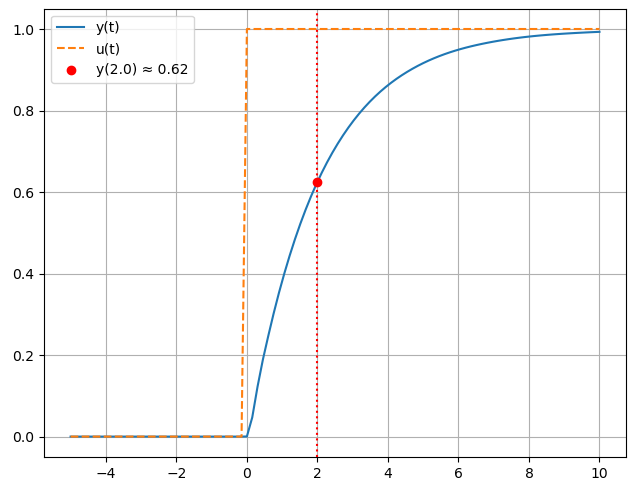
\includegraphics[scale=0.62]{../figures/first_degree_step_response.png}
	\end{center}
	che risulta effettivamente abbastanza vicino al $\sim 63.2 \%$.
\end{minipage}

\subsubsection{Tempo di assestamento}
Un'altro valore di interesse è il \textbf{tempo di assestamento} alla percentuale $i$, inteso come il tempo che serve a un sistema dinamico per rimanere una fascia $\pm i \%$ attorno al valore di regime.

Ad esempio, se vogliamo calcolare il tempo di assestamento al $5\%$, possiamo dire:
$$
y(t) = G(0) \left( 1 - e^{-\frac{t_{ss}}{T}} \right) = 0.95 \cdot G(0) \implies 0.05 = e^{-\frac{t_{ss}}{T}}
$$
da cui:
$$
t_{ss} = T \cdot \ln(20) \approx 3T
$$
cioè 3 volte il tempo caratterstico, come risultava abbastanza chiaro dalla tabella del paragrafo precedente.

\subsection{Forme di Bode e di Evans}
Vediamo un'altra equazione differenziale, dove adesso compare la derivata dell'ingresso:
$$
a_1 \frac{dy}{dt} + a_0 y = b_1 \frac{du}{dt} + b_0 u
$$
Nel dominio di Laplace questa avrà l'aspetto:
$$
a_1 \cdot s Y(s) + a_0 \cdot Y(s) + b_1 \cdot s U(s) + b_0 \cdot U(s)
$$
da cui la funzione di trasferimento:
$$
\frac{Y(s)}{U(s)} = \frac{b_0 + b_1 s}{a_0 + a_1 s} = G(s)
$$

Nota questa funzione di trasferimento, possiamo riportare due forme standard di riscrittura, che ne evidenziano proprietà diverse:
\begin{itemize}
	\item \textbf{Forma di Bode:} evidenzia le costanti tempo del sistema dinamico.
		$$
		G(s) = \frac{b_0}{a_0} \frac{1 + s \cdot \frac{b_1}{b_0}}{1 + s \cdot \frac{a_1}{a_0}} = G(0) \cdot \frac{1 + s \cdot \tau_z}{1 + s \cdot \tau}
		$$
		Notiamo che l'effetto della derivata dell'ingresso è stato quello di portare un termine $s$ al numeratore, e quindi quello di introdurre uno zero (a $-\frac{b_0}{b_1}$) nella funzione di trasferimento (zero per cui abbiamo introdotto il tempo caratteristico $\tau_z$).
	\item \textbf{Forma di Evans:} evidenzia le singolarità dinamiche del sistema, ovvero poli e zeri:
		$$
		G(s) = \frac{b_1}{a_1} \cdot \frac{s + \frac{b_0}{b_1}}{s + \frac{a_0}{a_1}}
		$$
\end{itemize}

Ad esempio, riguardo alla funzione di trasferimento dell'esempio 12.1.1, che ricordiamo essere:
$$
G(s) = \frac{\frac{b_0}{a_0}}{s + \frac{a_0}{a_1}}
$$
possiamo dire che si trova già in \textit{forma di Evans}, in quanto al denominatore è esplicitato l'unico polo.

Per ricavare la forma di Bode, invece, vorremo esporre il termine tempo caratteristico $\tau = \frac{a_1}{a_0}$:
$$
G(s) = \frac{b_0}{a_0} \cdot \frac{1}{1 + s \cdot \frac{a_1}{a_0}}
$$
che è nuovamente:
$$
= G(0) \cdot \frac{1}{1 + s \cdot \tau}
$$

\subsection{Sistemi del secondo ordine}
Abbiamo visto finora sistemi del primo ordine risolti tramite la trasformata di Laplace.
Vediamo adesso il caso dei sistemi del secondo ordine, che ci permettono di modellizzare una vasta gamma di fenomeni di interesse ingegneristico:
$$
a_2 \frac{d^2 y}{dt^2} + a_1 \frac{dy}{dt} + a_0 y = b_0 u
$$
complicando la situazione con condizioni iniziali non nulle ($y(0), y'(0) \neq 0$).

Applichiamo quindi Laplace alle due derivate successive:
$$
\mathcal{L} \left\{ \frac{dy}{dt} \right\} = s \cdot Y(s) - y(0)
$$
$$
\mathcal{L} \left\{ \frac{d^2y}{dt^2} \right\} = s \left( Y(s) - y(0) \right) - y'(0)
$$
da cui ricaviamo la forma:
$$
a_2 \cdot \left( s^2 \cdot Y(s) - s \cdot y(0) - y'(0) \right) + a_1 \cdot \left( s \cdot Y(s) - y(0) \right) + a_0 \cdot Y(s) = b_0 \cdot U(s)
$$

Esplicitando $Y(s)$ si otterrà:
$$
Y(s) = \frac{a_2 s \cdot y(0) + a_2 \cdot y'(0) + a_1 \cdot y(0)}{a_0 + a_1 s + a_2 s^2} + \frac{b_0}{a_0 + a_1 s + a_2 s^2} U(s) 
$$
dove riconosciamo che il primo termine rappresenta la \textbf{risposta libera} e il secondo la \textbf{risposta forzata} del sistema. 

Decidiamo di concentrarci sulla risposta forzata, ricavando la funzione di trasferimento:
$$
G(s) = \frac{Y(s)}{U(s)} = \frac{b_0}{a_2 s^2 + a_1 s + a_0} = \frac{ \frac{b_0}{a_2} }{s^2 + \frac{a_1}{a_2}s + \frac{a_0}{a_2}}
$$
da cui i poli al denominatore:
$$
p_{1, 2} = - \frac{-a_1 \pm \sqrt{a_1^2 - 4 a_0 a_2}}{2 a_2}
$$
da cui notiamo che 1) non ci interessa di considerare per i polinomi il polinomio monico, in quanto la loro posizione non cambierà e 2) prendiamo il segno $-$, in quanto vogliamo scrivere:
$$
G(s) = \frac{ \frac{b_0}{a_2} }{(s + p_1) (s + p_2)}
$$

Potremo quindi individuare il \textbf{determinante}:
$$
\Delta = a_1^2 - 4a_0a_2
$$
sulla base del quale distinguiamo 3 situazioni:
\begin{itemize}
	\item $\Delta > 0$, si hanno 2 poli \textbf{reali distinti}.
	\item $\Delta = 0$, si hanno 2 poli \textbf{reali coincidenti};
	\item $\Delta < 0$, si hanno 2 poli \textbf{complessi coniugati};
\end{itemize}
Vediamo nel dettaglio queste situazioni.

\subsubsection{$\mathbf{\Delta > 0}$, 2 poli reali distinti}
Risulta immediato che:
$$G(0) = \frac{b_0}{a_0}$$
e definiamo poi:
$$
\quad T_1 = \frac{1}{p_1}, \quad T_2 = \frac{1}{p_2}
$$

Vogliamo innanzitutto vedere come portarci nelle forme di Bode e di Evans.
Prima di tutto, però, dimostriamo due importanti proprietà:
\begin{enumerate}
	\item $p_1 \cdot p_2 = \frac{1}{T_1 \cdot T_2} = \frac{a_0}{a_2}$ \par\smallskip 
		Il lato sinistro è chiaro dalla definizione di $T_1$ e $T_2$.
		Per dimostrare il lato destro calcoliamo direttamente $p_1 \cdot p_2$:
		$$
		p_1 \cdot p_2 = \left( - \frac{-a_1 + \sqrt{a_1^2 - 4 a_0 a_2}}{2 a_2} \right) \left( - \frac{-a_1 - \sqrt{a_1^2 - 4 a_0 a_2}}{2 a_2} \right)
		$$
		$$
		= \frac{1}{4a_2^2} \left( a_1^2 - a_1^2 + 4a_2a_0 \right) = \frac{a_2 a_0}{a_2^2} = \frac{a_0}{a_2}
		$$ \qed
		
	\item $p_1 + p_2 = \frac{1}{T_1} + \frac{1}{T_2} = \frac{a_1}{a_2}$ \par\smallskip
		Anche qui il lato sinistro è chiaro dalla definizione di $T_1$ e $T_2$.
		Per dimostrare il lato destro procediamo nuovamente per calcolo diretto:
		$$
		p_1 + p_2 = - \frac{-a_1 + \sqrt{a_1^2 - 4 a_0 a_2}}{2 a_2} + \left( - \frac{-a_1 - \sqrt{a_1^2 - 4 a_0 a_2}}{2 a_2} \right) = \frac{a_1}{2 a_2} + \frac{a_1}{2 a_2} = \frac{a_1}{a_2}
		$$ \qed
\end{enumerate}

Vediamo allora le forme standard:
\begin{itemize}
	\item \textbf{Forma di Bode:} è analoga a quella vista nel caso lineare, cioè:
	$$
	G(s) = G(0) \cdot \frac{1}{(1 + s \cdot T_1)(1 + s \cdot T_2)}
	$$
	la validità di questa si ricava a moltiplicando e dividendo per $T_1 T_2$ e applicando la proprietà 1:
	$$
	= \frac{b_0}{a_0} \cdot \frac{1}{T_1 T_2 (\frac{1}{T_1} + s)(\frac{1}{T_2} + s)} = \frac{b_0}{a_0} = \frac{b_0}{a_0} \cdot \frac{a_0}{a_2} \cdot \frac{1}{(s + p_1)(s + p_2)} = \frac{\frac{b_0}{a_2}}{(s + p_1)(s + p_2)}
	$$ 
	che riconosciamo essere la forma che abbiamo usato finora.
	\item \textbf{Forma di Evans:} è la forma a poli espliciti che avevamo già trovato:
	$$
	G(s) = \frac{\frac{b_0}{a_2}}{(s + p_1)(s + p_2)}
	$$
\end{itemize}

\par\medskip

Vediamo quindi la \textbf{risposta al gradino}:
$$
Y(s) = G(s) \cdot U(s) = \frac{\frac{b_0}{a_2}}{(s + \frac{1}{T_1})(s + \frac{1}{T_2}) \cdot s} = \frac{A}{s} + \frac{B}{s + \frac{1}{T_1}} + \frac{C}{s + \frac{1}{T_2}}
$$
dove si è adottata questa forma \textit{"ibrida"} di Evans, dove manteniamo esplicite le costanti tempo.

Calcoliamo quindi i residui:
$$
A = \lim_{s \rightarrow 0} \frac{\frac{b_0}{a_2}}{(s + \frac{1}{T_1})(s + \frac{1}{T_2})} = \frac{b_0}{a_2} \cdot T_1 \cdot T_2 = \frac{b_0 \cdot a_2}{a_2 \cdot a_0} = \frac{b_0}{a_0} = G(0)
$$
sfruttando la proprietà 1 riportata prima.
Si ha poi:
$$
B = \lim_{s \rightarrow - \frac{1}{T_1}} \frac{\frac{b_0}{a_2}}{s (s + \frac{1}{T_2})} 
= \frac{b_0}{a_2} \cdot \frac{1}{-\frac{1}{T_1} (\frac{1}{T_2} - \frac{1}{T_1})} 
= \frac{b_0 \cdot T_1^2 T_2}{a_2 (T_2 - T_1)} 
= \frac{T_1}{T_2 - T_1} \cdot G(0)
$$
$$
C = \lim_{s \rightarrow - \frac{1}{T_2}} \frac{\frac{b_0}{a_2}}{s (s + \frac{1}{T_1})} 
= \frac{b_0}{a_2} \cdot \frac{1}{-\frac{1}{T_2} (\frac{1}{T_1} - \frac{1}{T_2})} 
= \frac{b_0 \cdot T_1 T_2^2}{a_2 (T_2 - T_1)} 
= -\frac{T_2}{T_2 - T_1} \cdot G(0)
$$

Calcoliamo quindi l'antitrasformata:
$$
y(t) = \mathcal{L}^{-1} \{ G(s) \cdot U(s) \} = G(0) \cdot \left( 1 + \frac{T_1 e^{-\frac{t}{T_1}} - T_2 e^{-\frac{t}{T_2}}}{T_2 - T_1} \right) \cdot H(t)
$$

\noindent
\begin{minipage}{\textwidth}
vediamo il grafico di una classica funzione $y(t)$ di questo tipo, che viene detta anche \textbf{sovrasmorzata}:
\begin{center}
	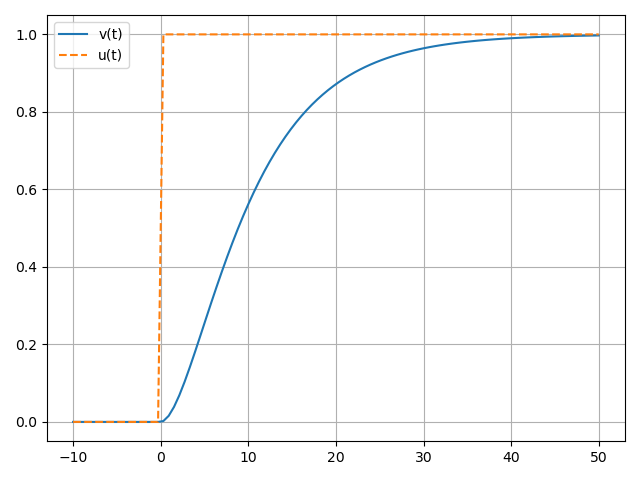
\includegraphics[scale=0.66]{../figures/second_degree_overdamped.png}
\end{center}
\end{minipage}

Notiamo che il grafico è qualitativamente simile a quello ottenuto da un sistema del primo ordine, anche se dobbiamo distinguere non una ma due costanti di tempo, $T_1$ e $T_2$.

\end{document}


\documentclass[a4paper,11pt]{article}
\usepackage[a4paper, margin=8em]{geometry}

% usa i pacchetti per la scrittura in italiano
\usepackage[french,italian]{babel}
\usepackage[T1]{fontenc}
\usepackage[utf8]{inputenc}
\frenchspacing 

% usa i pacchetti per la formattazione matematica
\usepackage{amsmath, amssymb, amsthm, amsfonts}

% usa altri pacchetti
\usepackage{gensymb}
\usepackage{hyperref}
\usepackage{standalone}

% imposta il titolo
\title{Appunti Fondamenti di Automatica}
\author{Luca Seggiani}
\date{2025}

% disegni
\usepackage{pgfplots}
\pgfplotsset{width=10cm,compat=1.9}

% imposta lo stile
% usa helvetica
\usepackage[scaled]{helvet}
% usa palatino
\usepackage{palatino}
% usa un font monospazio guardabile
\usepackage{lmodern}

% tikz in sans
\tikzset{every picture/.style={/utils/exec={\sffamily}}}

\renewcommand{\rmdefault}{ppl}
\renewcommand{\sfdefault}{phv}
\renewcommand{\ttdefault}{lmtt}

% circuiti
\usepackage{circuitikz}
\usetikzlibrary{babel}

% disponi il titolo
\makeatletter
\renewcommand{\maketitle} {
	\begin{center} 
		\begin{minipage}[t]{.8\textwidth}
			\textsf{\huge\bfseries \@title} 
		\end{minipage}%
		\begin{minipage}[t]{.2\textwidth}
			\raggedleft \vspace{-1.65em}
			\textsf{\small \@author} \vfill
			\textsf{\small \@date}
		\end{minipage}
		\par
	\end{center}

	\thispagestyle{empty}
	\pagestyle{fancy}
}
\makeatother

% disponi teoremi
\usepackage{tcolorbox}
\newtcolorbox[auto counter, number within=section]{theorem}[2][]{%
	colback=blue!10, 
	colframe=blue!40!black, 
	sharp corners=northwest,
	fonttitle=\sffamily\bfseries, 
	title=Teorema~\thetcbcounter: #2, 
	#1
}

% disponi definizioni
\newtcolorbox[auto counter, number within=section]{definition}[2][]{%
	colback=red!10,
	colframe=red!40!black,
	sharp corners=northwest,
	fonttitle=\sffamily\bfseries,
	title=Definizione~\thetcbcounter: #2,
	#1
}

% disponi problemi
\newtcolorbox[auto counter, number within=section]{problem}[2][]{%
	colback=green!10,
	colframe=green!40!black,
	sharp corners=northwest,
	fonttitle=\sffamily\bfseries,
	title=Problema~\thetcbcounter: #2,
	#1
}

% disponi codice
\usepackage{listings}
\usepackage[table]{xcolor}

\lstdefinestyle{codestyle}{
		backgroundcolor=\color{black!5}, 
		commentstyle=\color{codegreen},
		keywordstyle=\bfseries\color{magenta},
		numberstyle=\sffamily\tiny\color{black!60},
		stringstyle=\color{green!50!black},
		basicstyle=\ttfamily\footnotesize,
		breakatwhitespace=false,         
		breaklines=true,                 
		captionpos=b,                    
		keepspaces=true,                 
		numbers=left,                    
		numbersep=5pt,                  
		showspaces=false,                
		showstringspaces=false,
		showtabs=false,                  
		tabsize=2
}

\lstdefinestyle{shellstyle}{
		backgroundcolor=\color{black!5}, 
		basicstyle=\ttfamily\footnotesize\color{black}, 
		commentstyle=\color{black}, 
		keywordstyle=\color{black},
		numberstyle=\color{black!5},
		stringstyle=\color{black}, 
		showspaces=false,
		showstringspaces=false, 
		showtabs=false, 
		tabsize=2, 
		numbers=none, 
		breaklines=true
}

\lstdefinelanguage{javascript}{
	keywords={typeof, new, true, false, catch, function, return, null, catch, switch, var, if, in, while, do, else, case, break},
	keywordstyle=\color{blue}\bfseries,
	ndkeywords={class, export, boolean, throw, implements, import, this},
	ndkeywordstyle=\color{darkgray}\bfseries,
	identifierstyle=\color{black},
	sensitive=false,
	comment=[l]{//},
	morecomment=[s]{/*}{*/},
	commentstyle=\color{purple}\ttfamily,
	stringstyle=\color{red}\ttfamily,
	morestring=[b]',
	morestring=[b]"
}

% disponi sezioni
\usepackage{titlesec}

\titleformat{\section}
	{\sffamily\Large\bfseries} 
	{\thesection}{1em}{} 
\titleformat{\subsection}
	{\sffamily\large\bfseries}   
	{\thesubsection}{1em}{} 
\titleformat{\subsubsection}
	{\sffamily\normalsize\bfseries} 
	{\thesubsubsection}{1em}{}

% disponi alberi
\usepackage{forest}

\forestset{
	rectstyle/.style={
		for tree={rectangle,draw,font=\large\sffamily}
	},
	roundstyle/.style={
		for tree={circle,draw,font=\large}
	}
}

% disponi algoritmi
\usepackage{algorithm}
\usepackage{algorithmic}
\makeatletter
\renewcommand{\ALG@name}{Algoritmo}
\makeatother

% disponi numeri di pagina
\usepackage{fancyhdr}
\fancyhf{} 
\fancyfoot[L]{\sffamily{\thepage}}

\makeatletter
\fancyhead[L]{\raisebox{1ex}[0pt][0pt]{\sffamily{\@title \ \@date}}} 
\fancyhead[R]{\raisebox{1ex}[0pt][0pt]{\sffamily{\@author}}}
\makeatother

\begin{document}

% sezione (data)
\section{Lezione del 27-03-25}

% stili pagina
\thispagestyle{empty}
\pagestyle{fancy}

% testo
\subsubsection{$\mathbf \Delta = 0$, poli reali coincidenti}
Vediamo il caso di poli reali coincidenti, cioè $p_1 = p_2$.
Notiamo che questo caso è puramente teorico, in quanto la risposta di un sistema reale sarà necessariamente leggermente sottosmorzata o leggermente sovrasmorzata.

Potremo quindi dire:
$$
p_1 = p_2 = p, \quad T )= \frac{1}{p}
$$
e si avrà quindi l'unica proprietà:
$$
T^2 = \frac{1}{p^2} = \frac{a_2}{a_0}
$$
che deriva direttamente dalle precedenti.

Le forme standard saranno allora le seguenti:
\begin{itemize}
	\item \textbf{Forma di Bode:} questa si ricaverà moltiplicando sopra e sotto per $T^2$ e applicando la proprietà:
$$
G(s) = \frac{ \frac{b_0}{a_2} }{(s + \frac{1}{T})^2} = \frac{ \frac{b_0}{a_0} T^2 }{(1 + s T)^2} = \frac{ \frac{b_0}{a_2} \cdot \frac{a_2}{a_0} }{(1 + sT)^2} = G(0) \cdot \frac{1}{(1 + sT)^2}  
$$
che mette ancora in evidenza il guadagno $G(0)$.
	\item \textbf{Forma di Evans:} è la stessa che abbiamo usato finora, cioè:
$$
G(s) = \frac{ \frac{b_0}{a_2} }{ (s + p)^2 }
$$
sull'unico polo $p$.
\end{itemize}

Vediamo quindi la \textbf{risposta al gradino}, adottando la stessa forma \textit{"ibrida"} di Evans della scorsa lezione:
$$
Y(s) = G(s) \cdot U(s) = \frac{ \frac{b_0}{a_2} }{ \left( s + \frac{1}{T} \right)^2 } \cdot \frac{1}{s} = \frac{A}{s} + \frac{B}{s + \frac{1}{T}} + \frac{C}{\left( s + \frac{1}{T} \right)^2}
$$

Calcoliamo quindi i residui:
$$
A = \lim_{s \rightarrow 0} \frac{ \frac{b_0}{a_2} }{ \left( s + \frac{1}{T} \right)^2 } = \frac{b_0 \cdot T^2}{a_2} = \frac{b_0}{a_0} = G(0)
$$
$$
C = \lim_{s \rightarrow - \frac{1}{T}} \frac{b_0}{a_2} \cdot \frac{1}{s} = - \frac{b_0 \cdot T}{a_2} = - \frac{b_0}{a_0} \cdot \frac{a_0}{a_2} \cdot T = - G(0) \cdot \frac{T}{T^2} = -\frac{G(0)}{T}
$$
Per calcolare il residuo in $B$ sfruttiamo la proprietà che troviamo sempre, dall'annullamento dei termini in $s^2$ di $A$ e $B$ al numeratore:
$$
A + B = 0 \implies B = -A = -G(0)
$$

Calcoliamo quindi l'antitrasformata:
$$
y(t) = \mathcal{L}^{-1} \{G(s) \cdot U(s)\} = G(0) \cdot \left( 1 - e^{-\frac{t}{T}} \left( 1 + \frac{t}{T} \right) \right) \cdot H(t)
$$
dove per il termine quadrato si ha:
$$
\mathcal{L}^{-1} \left\{ \frac{ k }{ \left( s + \frac{1}{T} \right)^2 } \right\} = k \, t e^{-\frac{t}{T}}
$$
sfruttando la proprietà:
$$
F(s - a) = \mathcal{L} \{ e^{at} \cdot f(t) \}
$$
presa $f(t) = \frac{1}{s^2}$ e $a = -\frac{1}{T}$.

\subsubsection{$\mathbf \Delta < 0$, poli complessi coniugati}
Vediamo infine il caso con poli complessi coniugati.
Avremo quindi che questi rispettano la forma:
$$
p_{1,2} =  - \left( \alpha \pm i \beta \right)
$$
con:
$$
\alpha = -\frac{a_1}{2a_2}, \quad \beta = \sqrt{ \frac{a_0}{a_2} - \left( \frac{a_1}{2 a_2} \right)^2 } = \sqrt{ \frac{a_0}{a_2} \left( 1 - \frac{a_1^2}{4 a_2 a_0} \right) }
$$
che derivano direttamente da $p_1$ e $p_2$ come li avevamo definiti con la formula quadratica (portando $2 a_2$ dentro per $\beta$, che è il termine radicale col radicando cambiato di segno).

Possiamo ricavare due valori fisicamente significativi, che sono la \textbf{pulsazione di risonanza}:
$$
\omega = \sqrt{\frac{a_0}{a_2}}
$$
e lo \textbf{smorzamento}:
$$
\xi = \frac{a_1}{2 \sqrt{a_0 a_2}}
$$
sapendo che questa situazione darà solitamente comportamenti oscillatori smorzati o meno (non smorzati se $a_1 = 0$).

Varrà allora, rispetto ai poli:
\[
	\begin{cases}
		\alpha = -\xi \omega = - \frac{a_1}{2 \sqrt{a_0 a_2}} \sqrt{ \frac{a_0}{a_2} } = -\frac{a_1}{2 a_2} \\
		\beta = \omega \sqrt{1 - \xi^2} = \sqrt{ \frac{a_0}{a_2} } \sqrt{ 1 - \frac{a_1^2}{4 a_0 a_2} } = \sqrt{ \frac{a_0}{a_2} \left( 1 - \frac{a_1^2}{4 a_0 a_2} \right) }
	\end{cases}
\]

Potremo quindi adottare le forme standard:
\begin{itemize}
	\item \textbf{Forma di Bode:} questa sarà:
$$
G(s) = G(0) \cdot \frac{ 1 }{ \frac{1}{\omega^2} \cdot s^2 + 2 \frac{\xi}{\omega} \cdot s + 1 }
$$
notando che:
\[
	\begin{cases}
		2 \frac{\xi}{\omega} = 2 \frac{a_1}{2 \sqrt{a_0 a_2}} \cdot \sqrt{\frac{a_2}{a_0}} = \frac{a_1}{a_0} \\
		\frac{1}{\omega^2} = \frac{a_2}{a_0}
	\end{cases}
\]
e quindi:
$$
G(s) = \frac{ G(0) }{ \frac{1}{\omega^2} \cdot s^2 + 2 \frac{\xi}{\omega} \cdot s + 1 } = \frac{ \frac{b_0}{a_0} }{ 1 + \frac{a_1}{a_0} s + \frac{a_2}{a_0} s^2} = \frac{b_0}{a_0 + a_1 s + a_2 s^2}
$$
cioè equivale alla forma standard.
	\item \textbf{Forma di Evans:} questa sarà:
$$
G(s) = \frac{ \frac{b_0}{a_2} }{ s^2 + 2 \xi \omega \cdot s + \omega^2 }
$$
cioè la stessa di sopra moltiplicata sopra e sotto per $\omega^2$.
\end{itemize}

Vediamo quindi la \textbf{risposta al gradino}:


\subsubsection{Esempio: modello a quarto di automobile}
Prendiamo come esempio di sistema del secondo ordine quello del \textbf{quarto di automobile}, inteso come il sistema formato dalla massa dell'automobile $M_s$, che agisce sulla sospensione (di costante elastica $k_s$) e sull'ammortizzatore (di smorzamento $c$), a loro volta collegati al pneumatico di massa $M_n$, che agisce anch'esso da sospensione (di costante elastica $k_p$) per il collegamento alla strada.

Prendiamo $x_s$ come la posizione verticale dell'auto, $x_n$ come la posizione verticale del pneumatico, e $x_f$ come la posizione verticale della strada (che \textit{varia} mentre la vettura si muove sul tracciato stradale, in base alle asperità stesse dell'asfalto).

Possiamo riportare la costante elastica del pneumatico (di per sé complicata da calcolare, e comunque solitamente abbastanza grande da essere considerata come perfettamente solida) alla sospensione, considerando quindi la sola costante elastica $k_s$ della sospensione.

Prendiamo quindi la posizione verticale dell'automobile $x_s$ come l'uscita del sistema, e la posizione verticale della strada $x_f$ come l'entrata.

Chiamando poi $L_r$ la lunghezza della molla a riposo, potremmo impostare l'equazione differenziale come:
$$
M_s \frac{d^2 x_s}{dt^2} = c \frac{d ( x_f - x_s )}{dt} + k_s (x_f - x_s) + k_s L_r - M_s g
$$
dove il termine $k_s L_r$ deriva effettivamente dal fatto che la molla della sospensione risponde alla variazione della lunghezza a riposo della molla:
$$
F_s \propto  L_r - (x_s - x_f) = x_f - x_s + L_r
$$
mentre tutti i termini derivati non risentono di questa $L_r$ e quindi chiaramente la ignorano.

Dividiamo quindi la differenziale in una soluzione particolare, o di equilibrio, $\overline{x}_s$, e in una soluzione generale $\Delta x_s$:
$$
x_s = \Delta x_s + \overline{x}_s
$$
La condizione di equilibrio di questo sistema sarà quindi, imponendo derivate nulle:
$$
\overline{x}_s = L_r - \frac{M_s g}{k_s}
$$

Potremo allora prendere l'omogenea per il calcolo della soluzione generale:
$$
M_s \frac{d^2 \Delta x_s}{dt^2} = c \frac{d ( x_f - \Delta x_s )}{dt} + k_s (x_f - \Delta x_s)
$$
Raggruppando ingressi e uscite (rispettivamente, $\Delta x_s$ e $x_f$) si ha:
$$
M_s \frac{d^2 \Delta x_s}{dt^2} + c \frac{d \Delta x_s}{dt} + k_s \Delta x_s = c \frac{dx_f}{dt} + k_s x_f
$$
da cui, portandosi, al dominio di Laplace:
$$
\left( s^2 M_s + cs + k_s \right) \Delta x_s = ( cs + k_s ) x_f
$$
troviamo la funzione di trasferimento $G(s)$:
$$
G(s) = \frac{\Delta x_s}{x_f} = \frac{c s + k_s}{s^2 M_s + c s + k_s}
$$

La funzione di trasferimento ha uno zero e due poli.
Possiamo intanto ricavarci pulsazione ($\omega$) e smorzamento ($\xi$):
$$
\omega = \frac{k_s}{M_s}, \quad \xi = \frac{c}{2 \sqrt{k_s M_s}}
$$

\end{document}


\documentclass[a4paper,11pt]{article}
\usepackage[a4paper, margin=8em]{geometry}

% usa i pacchetti per la scrittura in italiano
\usepackage[french,italian]{babel}
\usepackage[T1]{fontenc}
\usepackage[utf8]{inputenc}
\frenchspacing 

% usa i pacchetti per la formattazione matematica
\usepackage{amsmath, amssymb, amsthm, amsfonts}

% usa altri pacchetti
\usepackage{gensymb}
\usepackage{hyperref}
\usepackage{standalone}

% imposta il titolo
\title{Appunti Fondamenti di Automatica}
\author{Luca Seggiani}
\date{2025}

% disegni
\usepackage{pgfplots}
\pgfplotsset{width=10cm,compat=1.9}

% imposta lo stile
% usa helvetica
\usepackage[scaled]{helvet}
% usa palatino
\usepackage{palatino}
% usa un font monospazio guardabile
\usepackage{lmodern}

% tikz in sans
\tikzset{every picture/.style={/utils/exec={\sffamily}}}

\renewcommand{\rmdefault}{ppl}
\renewcommand{\sfdefault}{phv}
\renewcommand{\ttdefault}{lmtt}

% circuiti
\usepackage{circuitikz}
\usetikzlibrary{babel}

% disponi il titolo
\makeatletter
\renewcommand{\maketitle} {
	\begin{center} 
		\begin{minipage}[t]{.8\textwidth}
			\textsf{\huge\bfseries \@title} 
		\end{minipage}%
		\begin{minipage}[t]{.2\textwidth}
			\raggedleft \vspace{-1.65em}
			\textsf{\small \@author} \vfill
			\textsf{\small \@date}
		\end{minipage}
		\par
	\end{center}

	\thispagestyle{empty}
	\pagestyle{fancy}
}
\makeatother

% disponi teoremi
\usepackage{tcolorbox}
\newtcolorbox[auto counter, number within=section]{theorem}[2][]{%
	colback=blue!10, 
	colframe=blue!40!black, 
	sharp corners=northwest,
	fonttitle=\sffamily\bfseries, 
	title=Teorema~\thetcbcounter: #2, 
	#1
}

% disponi definizioni
\newtcolorbox[auto counter, number within=section]{definition}[2][]{%
	colback=red!10,
	colframe=red!40!black,
	sharp corners=northwest,
	fonttitle=\sffamily\bfseries,
	title=Definizione~\thetcbcounter: #2,
	#1
}

% disponi problemi
\newtcolorbox[auto counter, number within=section]{problem}[2][]{%
	colback=green!10,
	colframe=green!40!black,
	sharp corners=northwest,
	fonttitle=\sffamily\bfseries,
	title=Problema~\thetcbcounter: #2,
	#1
}

% disponi codice
\usepackage{listings}
\usepackage[table]{xcolor}

\lstdefinestyle{codestyle}{
		backgroundcolor=\color{black!5}, 
		commentstyle=\color{codegreen},
		keywordstyle=\bfseries\color{magenta},
		numberstyle=\sffamily\tiny\color{black!60},
		stringstyle=\color{green!50!black},
		basicstyle=\ttfamily\footnotesize,
		breakatwhitespace=false,         
		breaklines=true,                 
		captionpos=b,                    
		keepspaces=true,                 
		numbers=left,                    
		numbersep=5pt,                  
		showspaces=false,                
		showstringspaces=false,
		showtabs=false,                  
		tabsize=2
}

\lstdefinestyle{shellstyle}{
		backgroundcolor=\color{black!5}, 
		basicstyle=\ttfamily\footnotesize\color{black}, 
		commentstyle=\color{black}, 
		keywordstyle=\color{black},
		numberstyle=\color{black!5},
		stringstyle=\color{black}, 
		showspaces=false,
		showstringspaces=false, 
		showtabs=false, 
		tabsize=2, 
		numbers=none, 
		breaklines=true
}

\lstdefinelanguage{javascript}{
	keywords={typeof, new, true, false, catch, function, return, null, catch, switch, var, if, in, while, do, else, case, break},
	keywordstyle=\color{blue}\bfseries,
	ndkeywords={class, export, boolean, throw, implements, import, this},
	ndkeywordstyle=\color{darkgray}\bfseries,
	identifierstyle=\color{black},
	sensitive=false,
	comment=[l]{//},
	morecomment=[s]{/*}{*/},
	commentstyle=\color{purple}\ttfamily,
	stringstyle=\color{red}\ttfamily,
	morestring=[b]',
	morestring=[b]"
}

% disponi sezioni
\usepackage{titlesec}

\titleformat{\section}
	{\sffamily\Large\bfseries} 
	{\thesection}{1em}{} 
\titleformat{\subsection}
	{\sffamily\large\bfseries}   
	{\thesubsection}{1em}{} 
\titleformat{\subsubsection}
	{\sffamily\normalsize\bfseries} 
	{\thesubsubsection}{1em}{}

% disponi alberi
\usepackage{forest}

\forestset{
	rectstyle/.style={
		for tree={rectangle,draw,font=\large\sffamily}
	},
	roundstyle/.style={
		for tree={circle,draw,font=\large}
	}
}

% disponi algoritmi
\usepackage{algorithm}
\usepackage{algorithmic}
\makeatletter
\renewcommand{\ALG@name}{Algoritmo}
\makeatother

% disponi numeri di pagina
\usepackage{fancyhdr}
\fancyhf{} 
\fancyfoot[L]{\sffamily{\thepage}}

\makeatletter
\fancyhead[L]{\raisebox{1ex}[0pt][0pt]{\sffamily{\@title \ \@date}}} 
\fancyhead[R]{\raisebox{1ex}[0pt][0pt]{\sffamily{\@author}}}
\makeatother

\begin{document}

% sezione (data)
\section{Lezione del 01-04-25}

% stili pagina
\thispagestyle{empty}
\pagestyle{fancy}

% testo
\noindent
\begin{minipage}{\textwidth}
\subsection{Dettaglio sulla risposta dei sistemi sottosmorzati}
Vediamo in particolare alcune grandezze di interesse nel caso di sistemi di secondo grado sottosmorzati:

\par\bigskip

\begin{center}
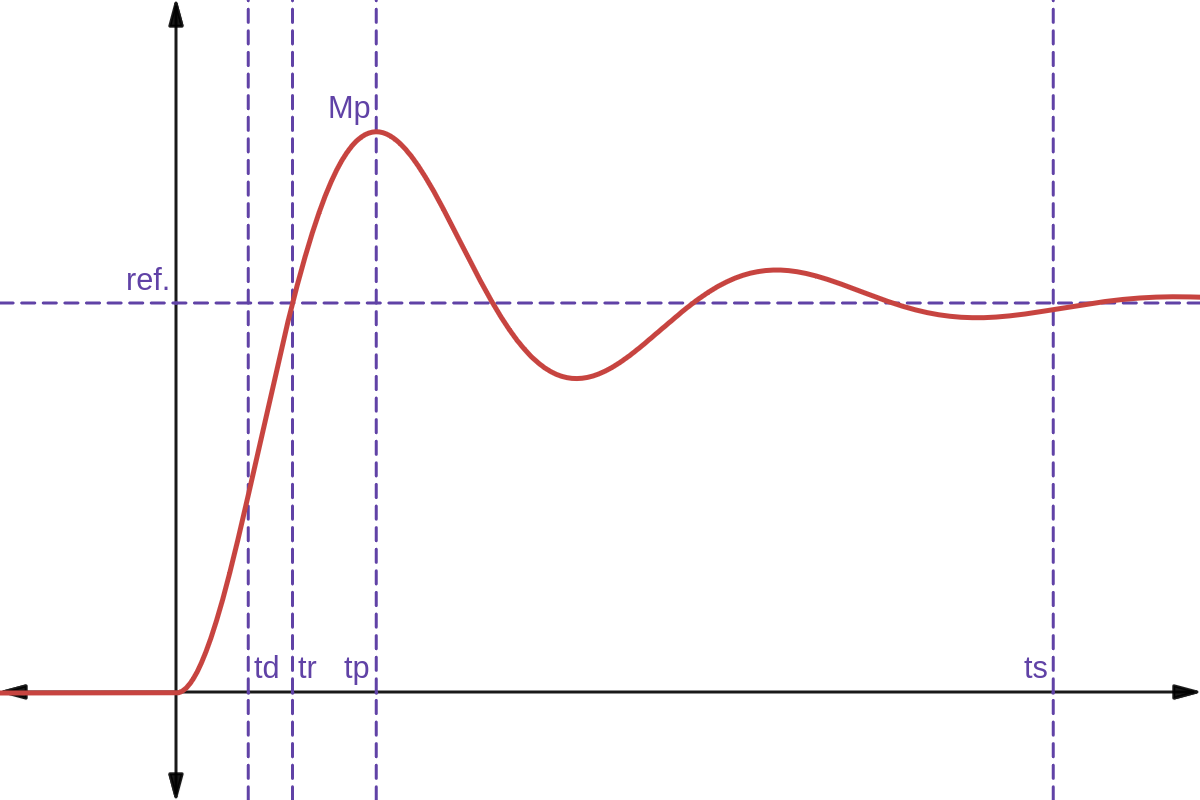
\includegraphics[scale=0.29]{../figures/damped_oscillator.png}
\end{center}
\end{minipage}

\par\bigskip

Abbiamo che una caratteristica del loro comportamento è la \textbf{sovraelongazione} al di sopra del valore bersaglio.
Chiamiamo quindi $M_p$ la \textit{massima sovraelongazione} sopra il livello di riferimento, e $t_p$ l'istante temporale in cui questa viene raggiunta.
Avremo poi il tempo $t_r$ \textit{di salita}, il momento in cui viene toccato per la prima volta il valore bersaglio, e il tempo $t_d$ \textit{di ritardo}, che viene impiegato a raggiungere il 50\% del valore bersaglio.
Infine, per valutare il comportamento oscillante dopo il transiente iniziale, consideriamo il tempo $t_s$ \textit{di assestamento}, oltre il quale il segnale resta in una certa (piccola) percentuale del valore bersaglio.

\noindent
\begin{minipage}{\textwidth}
Vediamo il comportamento generale dei sistemi di questo tipo al variare del valore di smorzamento $\xi = \frac{a_1}{2 \sqrt{a_0 a_2}}$:

\par\bigskip

\begin{center}
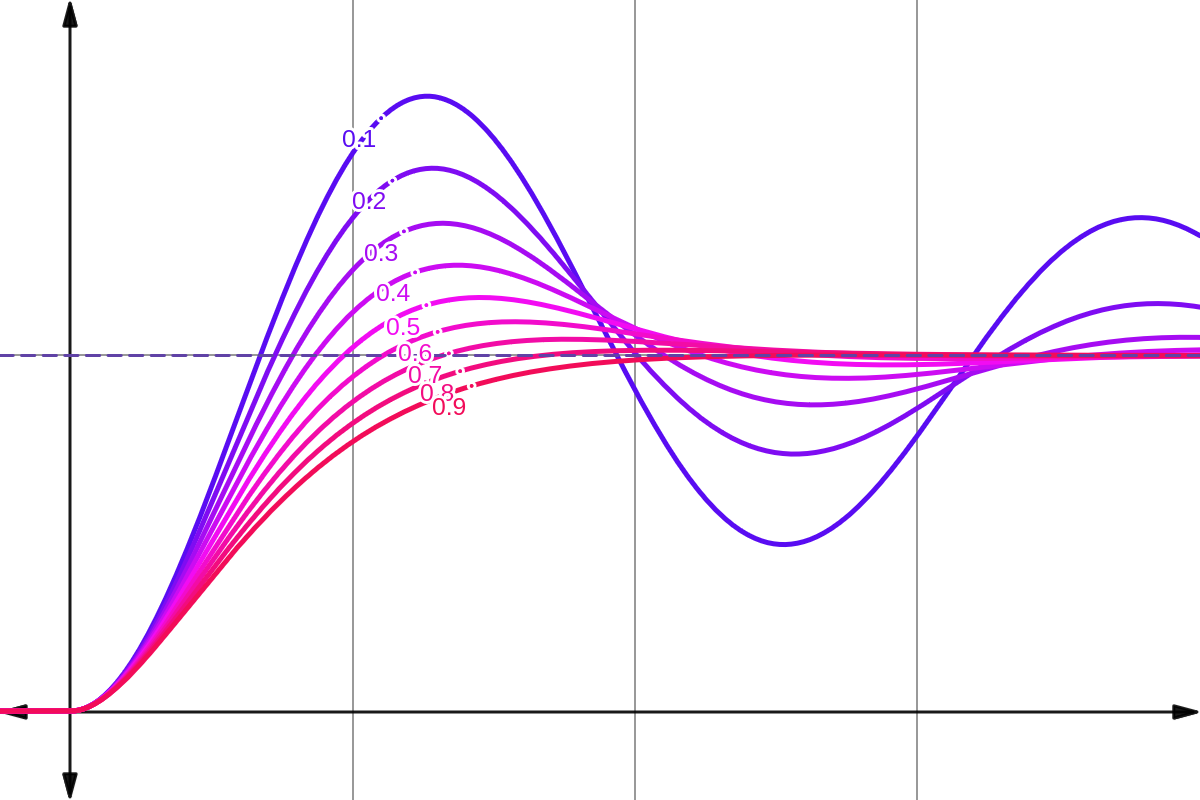
\includegraphics[scale=0.29]{../figures/damping_values.png}
\end{center}
\end{minipage}

\par\bigskip

Da dove notiamo che a valori di smorzamento maggiori si ha minore sovraelongamneto, ma anche maggiore tempo di salita.

Notiamo che possiamo considerare gli stessi parametri considerati sui sistemi sottosmorzati anche per sistemi criticamente smorzati o sovrasmorzati: infatti, se non per il tempo e per il punto di sovraelengazione, questi avranno valori ben definiti per qualsiasi sistema del second'ordine.

Tornando al dettaglio dei sistemi sottosmorzati, possiamo trovare le seguenti formule:
\begin{itemize}
	\item \textbf{Sovraelongazione:} si ha il picco in:
		$$
			S\% \ (M_p) \ = 100 e^{- \frac{\xi \pi}{\sqrt{1 - \xi^2}}}
		$$
		raggiunto all'istante:
		$$
			t_p = \frac{\pi}{\omega \sqrt{1 - \xi^2}}
		$$
	\item \textbf{Periodo di oscillazione:} possiamo considerare anche il periodo (e quindi la frequenza) delle oscillazioni, considerando il polo in $\beta$:
		$$
			T_o = \frac{2\pi}{\omega \sqrt{1 - x^2}}
		$$
		$$
			f_o = \frac{\omega \sqrt{1 - x^2}}{2\pi} 
		$$
	\item \textbf{Tempo di assestamento:} consideriamo questo come:
		$$
		t_s \approx -\frac{1}{\xi \omega} \ln(0.05)
		$$
	\item \textbf{Tempo di salita} consideriamo infine questo, con molta approssimazione, come:
		$$
		t_r \approx \frac{1.8}{\omega}
		$$
\end{itemize}

\subsubsection{Derivazione alternativa della funzione sottosmorzata}
Avevamo ricavato l'espressione:
$$
y(t) = \frac{b_0}{a_0} \left( 1 - e{\alpha t} \cos(\beta t) + \frac{\alpha}{\beta} e^{\alpha t} e^{\alpha t} \sin(\beta t) \right) \cdot H(t)
$$
per i sistemi del second'ordine sottosmorzati.
Vediamo come si può svolgere una derivazione, attraverso Laplace, per arrivare alla forma (equivalente):
$$
y(t) = G(0) \cdot \left( 1 - e^{-\xi \omega t} \cos\left(\omega \sqrt{1 - \xi ^2} \cdot t \right) - \frac{\xi}{\sqrt{1 - \xi^2}} e^{-\xi \omega t} \sin\left( \omega \sqrt{1 - \xi^2} \cdot t \right) \right)
$$
vediamo come questa evidenzia la dipendenza dal guadagno $G(0)$, e dai valori di pulsazione naturale $\omega$ e smorzamento $\xi$.

# fallo

Il lato destro dell'espressione trovata si può chiaramente riscrivere nella forma più concisa $ke^{-\sigma t} \sin(\omega t + \alpha)$. 
Usiamo allora le formule di traduzione in forma sinusoidale, di cui una dimostrazione nel caso cosinusoidale si trova a \url{https://github.com/seggiani-luca/appunti-fis/blob/main/master/master.pdf}:
\[
	c_1 \sin{\omega t} + c_2 \cos{\omega t}
	\Leftrightarrow
	k \sin(\omega t + \alpha)
\]
con:
\[
	\begin{cases}
		k 	= \sqrt{c_1^2 + c_2^2} \\ 
		\alpha = \tan^{-1}(\frac{c1}{c2})
	\end{cases}
\]

che darà quindi:
$$
y(t) = G(0) \cdot \left( 1 - e^{-\xi \omega t} \sqrt{1 + \frac{\xi^2}{1 + \xi^2}} \sin\left( \omega \sqrt{1 - \xi^2} \cdot t + \tan^{-1} \left( \frac{\sqrt{1 - \xi^2}}{\xi} \right) \right) \right) 
$$

\subsection{Stabilità nel modello a funzione di trasferimento}
Abbiamo lavorato finora col modello a funzione di trasferimento, definita come:
$$
G(s) = \frac{\sum_{i = 0}^m b_i s^i}{\sum_{i = 0}^n a_i s^i} = \frac{ b_m (s - z_1) (s - z_2) ... (s - z_m) }{ a_n (s - p_1) (s - p_2) ... (s - p_n) }
$$
con $z_i$ gli $m$ \textit{zeri}, $p_i$ gli $n$ \textit{poli}, e $n > m$.

Di questa avevamo individuato le due forme:
\begin{itemize}
	\item \textbf{Forma di Evans:} evidenzia poli e zeri:
		$$
G(s) = \frac{\sum_{i = 0}^m b_i s^i}{\sum_{i = 0}^n a_i s^i} = \frac{ b_m (s - z_1) (s - z_2) ... (s - z_m) }{ a_n (s - p_1) (s - p_2) ... (s - p_n) }
		$$
	\item \textbf{Forma di Bode:} evidenzia le costanti tempo: 
		$$
G(s) = K \frac{ (\tau_a s + 1) (\tau_b s + 1) ... (\tau_i s + 1) }{ (\tau_1 s + 1) (\tau_2 s + 1) ... (\tau_n s + 1) }
		$$
\end{itemize}

Definiamo quindi formalmente \textbf{poli}:
\begin{definition}{Polo}
	Un polo $a_i$ di una funzione di trasferimento $G(s)$ è un valore di $s$ per cui $G(s)$ tende ad infinito:
	$$
	F(s) = \frac{g(s)}{\prod_{i = 1}^x (s - a_i)^n_i}
	$$
	con $n_i$ ordine del polo.
\end{definition}
e \textbf{zeri}:
\begin{definition}{Zeri}
	Uno zero $a_i$ di una funzione di trasferimento $G(s)$ è un valore di $s$ per cui $G(s)$ tende a zero: 
	$$
	F(s) = \frac{\prod_{i = 1}^x (s - a_i)^m_i}{g(s)}
	$$
	con $m_i$ ordine dello zero.
\end{definition}

Quello che ci interesserà nella valutazione della \textbf{stabilità} dei sistemi sarà la posizione dei poli nel piano complesso.
In particolare, come avevamo detto per i modi nel modello a variabili di stato, poli a componente \textit{reale negativa} danno \textbf{stabilità asintotica}, poli a componente \textit{reale nulla} danno \textbf{stabilità marginale}, e poli a componente \textit{reale positiva} dano \textbf{instabilità}.
Inoltre la componente \textit{complessa} dà informazioni sull'oscillazione del sistema, con \textbf{oscillazioni smorzate} a componente \textit{complessa e reale non nulle}, e \textbf{oscillazioni continue} a componente \textit{reale nulla}.

Gli zeri, invece, non hanno effetto sulla stabilità.
Gli zeri a parte reale positiva hanno invece l'effetto di \textit{invertire} la risposta al gradino, almeno sul breve termine.

\subsubsection{Conversione da spazio di stato a funzione di trasferimento}
Dovrebbe ormai essere chiaro che lo spazio di stato e la funzione di trasferimento rappresentano due modi di modelizzare lo stesso tipo di fenomeni.
Vediamo quindi come passare dall'uno all'altro.

Partiamo dal modello a variabili di stato:
\[
	\begin{cases}
		x' = Ax + Bu \\
		y = Cx + Du
	\end{cases}
\]

Assumendo condizioni iniziali nulle, si ha:
\[
	\begin{cases}
		s X(s) = A X(s) + B U(s)  \\ 
		Y(s) = C X(s) + D U(s) 
	\end{cases} \implies
	\begin{cases}
		X(s) = (sI - A)^{-1} B U(s) \\
		Y(s) = \left( C(sI - A)^{-1} B + D \right) U(s)
	\end{cases}
\]
notando che $X, U$ sono vettori e $A, B$ matrici.

Si trova quindi la funzione di trasferimento:
$$
G(s) = \frac{Y(s)}{U(s)} = C(sI - A)^{-1} B + D
$$

\subsubsection{Forme canoniche di controllo}
Esistono un numero infinito di possibili modelli in spazio di stato che forniscono la stessa dinamica ingresso/uscita.

Aiuta avere alcune strutture standardizzate dei modelli in spazio di stato: queste sono le cosiddette forme canoniche.
Data la funzione di trasferimento di un sistema, è possibile ottenere ciascuna delle forme canoniche.
Data una particolare forma canonica, è poi possibile trasformarla in qualsiasi altra forma.

Consideriamo ad esempio il sistema definito da:
$$
y^{(n)} + a_1 y^{(n - 1)} + ... + a_{n - 1}y' + a_n y = b_0 u^{(n)} + b_1 u^{(n - 1)} + ... + b_{n - 1} u' + b_nu
$$

Prendendo la trasformata di Laplace da entrambi i lati si ha:
$$
Y(s) \left( s^n + a_1 s^{n - 1} + ... + a_{n - 1} s + a_n \right) = U(s) \left( b_0 s^n + b_1 s^{n - 1} + ... + b_{n - 1} s + b_n \right)
$$
da cui la funzione di trasferimento:
$$
G(s) = \frac{Y(s)}{U(s)} = \frac{ b_0 s^n + b_1 s^{n - 1} + ... + b_{n - 1} s + b_n}{s^n + a_1 s^{n - 1} + ... + a_{n - 1} s + a_n }
$$

Mentre avevamo già visto come la stessa forma in variabili di stato aveva l'aspetto:
\[
	\begin{cases}	
x' = \left(\begin{array}{@{}c | cccc@{}}
	0 & 1 & 0 & ... & 0 \\
	0 & 0 & 1 & ... & 0 \\
	... & ... & ... & ... & ... \\
	0 & 0 & 0 & ... & 1 \\
	\hline
	-a & ... & ... & ... & -a_{n - 1}
\end{array}\right)
x + \begin{pmatrix}
0 \\
... \\
0 \\
1
\end{pmatrix} u \\ 
y = \begin{pmatrix}
	b_0 - b_n a_0 & ... & b_{n - 1} - b_n a_{n - 1}	
\end{pmatrix} x + \begin{pmatrix}
b_n
\end{pmatrix} u
	\end{cases}
\]

# confronta

\end{document}


\documentclass[a4paper,11pt]{article}
\usepackage[a4paper, margin=8em]{geometry}

% usa i pacchetti per la scrittura in italiano
\usepackage[french,italian]{babel}
\usepackage[T1]{fontenc}
\usepackage[utf8]{inputenc}
\frenchspacing 

% usa i pacchetti per la formattazione matematica
\usepackage{amsmath, amssymb, amsthm, amsfonts}

% usa altri pacchetti
\usepackage{gensymb}
\usepackage{hyperref}
\usepackage{standalone}

% imposta il titolo
\title{Appunti Fondamenti di Automatica}
\author{Luca Seggiani}
\date{2025}

% disegni
\usepackage{pgfplots}
\pgfplotsset{width=10cm,compat=1.9}

% imposta lo stile
% usa helvetica
\usepackage[scaled]{helvet}
% usa palatino
\usepackage{palatino}
% usa un font monospazio guardabile
\usepackage{lmodern}

% tikz in sans
\tikzset{every picture/.style={/utils/exec={\sffamily}}}

\renewcommand{\rmdefault}{ppl}
\renewcommand{\sfdefault}{phv}
\renewcommand{\ttdefault}{lmtt}

% circuiti
\usepackage{circuitikz}
\usetikzlibrary{babel}

% disponi il titolo
\makeatletter
\renewcommand{\maketitle} {
	\begin{center} 
		\begin{minipage}[t]{.8\textwidth}
			\textsf{\huge\bfseries \@title} 
		\end{minipage}%
		\begin{minipage}[t]{.2\textwidth}
			\raggedleft \vspace{-1.65em}
			\textsf{\small \@author} \vfill
			\textsf{\small \@date}
		\end{minipage}
		\par
	\end{center}

	\thispagestyle{empty}
	\pagestyle{fancy}
}
\makeatother

% disponi teoremi
\usepackage{tcolorbox}
\newtcolorbox[auto counter, number within=section]{theorem}[2][]{%
	colback=blue!10, 
	colframe=blue!40!black, 
	sharp corners=northwest,
	fonttitle=\sffamily\bfseries, 
	title=Teorema~\thetcbcounter: #2, 
	#1
}

% disponi definizioni
\newtcolorbox[auto counter, number within=section]{definition}[2][]{%
	colback=red!10,
	colframe=red!40!black,
	sharp corners=northwest,
	fonttitle=\sffamily\bfseries,
	title=Definizione~\thetcbcounter: #2,
	#1
}

% disponi problemi
\newtcolorbox[auto counter, number within=section]{problem}[2][]{%
	colback=green!10,
	colframe=green!40!black,
	sharp corners=northwest,
	fonttitle=\sffamily\bfseries,
	title=Problema~\thetcbcounter: #2,
	#1
}

% disponi codice
\usepackage{listings}
\usepackage[table]{xcolor}

\lstdefinestyle{codestyle}{
		backgroundcolor=\color{black!5}, 
		commentstyle=\color{codegreen},
		keywordstyle=\bfseries\color{magenta},
		numberstyle=\sffamily\tiny\color{black!60},
		stringstyle=\color{green!50!black},
		basicstyle=\ttfamily\footnotesize,
		breakatwhitespace=false,         
		breaklines=true,                 
		captionpos=b,                    
		keepspaces=true,                 
		numbers=left,                    
		numbersep=5pt,                  
		showspaces=false,                
		showstringspaces=false,
		showtabs=false,                  
		tabsize=2
}

\lstdefinestyle{shellstyle}{
		backgroundcolor=\color{black!5}, 
		basicstyle=\ttfamily\footnotesize\color{black}, 
		commentstyle=\color{black}, 
		keywordstyle=\color{black},
		numberstyle=\color{black!5},
		stringstyle=\color{black}, 
		showspaces=false,
		showstringspaces=false, 
		showtabs=false, 
		tabsize=2, 
		numbers=none, 
		breaklines=true
}

\lstdefinelanguage{javascript}{
	keywords={typeof, new, true, false, catch, function, return, null, catch, switch, var, if, in, while, do, else, case, break},
	keywordstyle=\color{blue}\bfseries,
	ndkeywords={class, export, boolean, throw, implements, import, this},
	ndkeywordstyle=\color{darkgray}\bfseries,
	identifierstyle=\color{black},
	sensitive=false,
	comment=[l]{//},
	morecomment=[s]{/*}{*/},
	commentstyle=\color{purple}\ttfamily,
	stringstyle=\color{red}\ttfamily,
	morestring=[b]',
	morestring=[b]"
}

% disponi sezioni
\usepackage{titlesec}

\titleformat{\section}
	{\sffamily\Large\bfseries} 
	{\thesection}{1em}{} 
\titleformat{\subsection}
	{\sffamily\large\bfseries}   
	{\thesubsection}{1em}{} 
\titleformat{\subsubsection}
	{\sffamily\normalsize\bfseries} 
	{\thesubsubsection}{1em}{}

% disponi alberi
\usepackage{forest}

\forestset{
	rectstyle/.style={
		for tree={rectangle,draw,font=\large\sffamily}
	},
	roundstyle/.style={
		for tree={circle,draw,font=\large}
	}
}

% disponi algoritmi
\usepackage{algorithm}
\usepackage{algorithmic}
\makeatletter
\renewcommand{\ALG@name}{Algoritmo}
\makeatother

% disponi numeri di pagina
\usepackage{fancyhdr}
\fancyhf{} 
\fancyfoot[L]{\sffamily{\thepage}}

\makeatletter
\fancyhead[L]{\raisebox{1ex}[0pt][0pt]{\sffamily{\@title \ \@date}}} 
\fancyhead[R]{\raisebox{1ex}[0pt][0pt]{\sffamily{\@author}}}
\makeatother

\begin{document}

% sezione (data)
\section{Lezione del 02-04-25}

% stili pagina
\thispagestyle{empty}
\pagestyle{fancy}

% testo
\subsubsection{Esempio: conversione dalla forma a stato alla funzione di trasferimento}
Prendiamo l'esempio di una forma a variabili di stato arbitraria e riportiamola in funzione di trasferimento:
\[
	\begin{cases}
		x' = 
		\begin{pmatrix}
			0 & 1 & 0 \\ 0 & 0 & 1 \\ -1 & -2 & -3
		\end{pmatrix}
		x +
		\begin{pmatrix}
			10 \\ 0 \\ 0
		\end{pmatrix}
		u \\ 
		y =
		\begin{pmatrix}
			1 & 0 & 0
		\end{pmatrix}
		x
	\end{cases}
\]
Dalla matrice $A$ ricaviamo $sI - A$:
$$
sI - A =
\begin{pmatrix}
	s & -1 & 0 \\
	0 & s & -1 \\ 
	1 & 2 & s + 3
\end{pmatrix}
$$
da cui l'inversa:
$$
(sI - A)^{-1} =
\frac{1}{s^3 + 3s^2 + 2s + 1}
\begin{pmatrix}
	s^2 + 3s - 2 & s + 3 & 1 \\ 
	-1 & s^2 + 3s & s \\ 
	-s & -2s - 1 & s^2
\end{pmatrix}
$$
dove notiamo come sempre il denominatore è il polinomio dato da $a_n ... a_1$.
Applichiamo quindi la formula completa:
$$
G(s) = C (sI - A)^{-1} B \, ( + D ) = 
\begin{pmatrix}
	1 & 0 & 0
\end{pmatrix}
\frac{1}{s^3 + 3s^2 + 2s + 1}
\begin{pmatrix}
	s^2 + 3s - 2 & s + 3 & 1 \\ 
	-1 & s^2 + 3s & s \\ 
	-s & -2s - 1 & s^2
\end{pmatrix}
\begin{pmatrix}
	10 \\ 0 \\ 0
\end{pmatrix}
$$
$$
\begin{pmatrix}
	1 & 0 & 0
\end{pmatrix}
\frac{1}{s^3 + 3s^2 + 2s + 1}
\begin{pmatrix}
	10s^2 + 30s - 20 \\ 
	-10 \\
	-10s
\end{pmatrix}
= \frac{10s^2 + 30s - 20}{s^3 + 3s^2 + 2s + 1}
$$

\subsubsection{Matrici di trasferimento dei sistemi MIMO}
Abbiamo visto finora la funzione di trasferimento come una funzione scalare della variabile $s$.
Abbiamo in verità che questa può essere rappresentata in sistemi MIMO come:
$$
\mathbf{G}(s) = C (sI - A)^{-1} B =
\begin{pmatrix}
	g_{11}(s) & ... & g_{1m}(s) \\
	\vdots & \ddots & \vdots \\ 
	g_{p1}(s) & ... & g_{pm}(s) \\
\end{pmatrix}
$$
cioè una matrice che lega il trasferimento da ogni canale di ingresso a ogni canale di uscita, con $g_{ij}(s)$ funzione di trasferimento dal canale $u_j$ all'uscita $y_i$.

\subsubsection{Esempio: funzione di trasferimento della velocità di crociera}
Riprendiamo un'ennesima volta l'esempio 3.0.1, ricavandone la forma in funzione di trasferimento.
Avevamo che questo era rappresentato dal sistema:
\[
	\begin{cases}
		x' = \begin{pmatrix}
			0 & 1 \\ 0 & -\frac{\beta}{m}
		\end{pmatrix}	
		x + \begin{pmatrix}
			0 & 0 \\ \frac{\gamma}{m} & - g
		\end{pmatrix}
		u \\
		y = \begin{pmatrix}
			0 & 1
		\end{pmatrix}
		x
	\end{cases}
\]
da cui:
$$
sI - A = \begin{pmatrix}
	s & -1 \\
	0 & s + \frac{\beta}{m}
\end{pmatrix}, \quad
(sI - A)^{-1} =
\frac{1}{s\left( s + \frac{\beta}{m} \right)}
\begin{pmatrix}
	s + \frac{\beta}{m} & 1 \\
	0 & s
\end{pmatrix}
$$
Applicando la formula:
$$
\mathbf{G}(s) = C(sI - A)^{-1} B = \frac{1}{s\left(s + \frac{\beta}{m}\right)}
\begin{pmatrix}
	s \frac{\gamma}{m} - sg
\end{pmatrix}
= \begin{pmatrix}
	\frac{\gamma}{m \left( s + \frac{\beta}{m} \right)} &
	\frac{-g}{s + \frac{\beta}{m}}
\end{pmatrix}
$$

Avremo quindi una funzione di trasferimento $2\times 1$, dove le due entrate rappresentano rispettivamente l'effetto della propulsione del motore (che era $\gamma u$) e dell'accelerazione gravitazionale.
Visto che sulla seconda non si può agire, prenderemo in interesse la prima entrata:
$$
G(s) = \frac{\gamma}{m \left( s + \frac{\beta}{m} \right)}
$$

Di questa potremmo ad esempio prendere la risposta al gradino, che dalla linearità del sistema ci dà la risposta dell'automobile al controllo sull'acceleratore, trascurata l'accelerazione gravitazionale.

Avremo quindi:
$$
Y(s) = G(s) U(s) = \frac{\gamma}{m \left( s + \frac{\beta}{m} \right)} \frac{1}{s} = \frac{\alpha_1}{s + \frac{\beta}{m}} + \frac{\alpha_2}{s}
$$
che antitransforma in:
$$
y(t) = \left( \alpha_1 e^{-\frac{\beta}{m} t} + \alpha_2 \right) \cdot H(t)
$$
con:
$$
\alpha_1 = - \frac{\gamma}{\beta}, \quad \alpha_2 = \frac{\gamma}{\beta}
$$

\noindent
\begin{minipage}{\textwidth}
Abbiamo quindi che la risposta è la classica risposta al gradino di un sistema del prim'ordine:
\begin{center}
	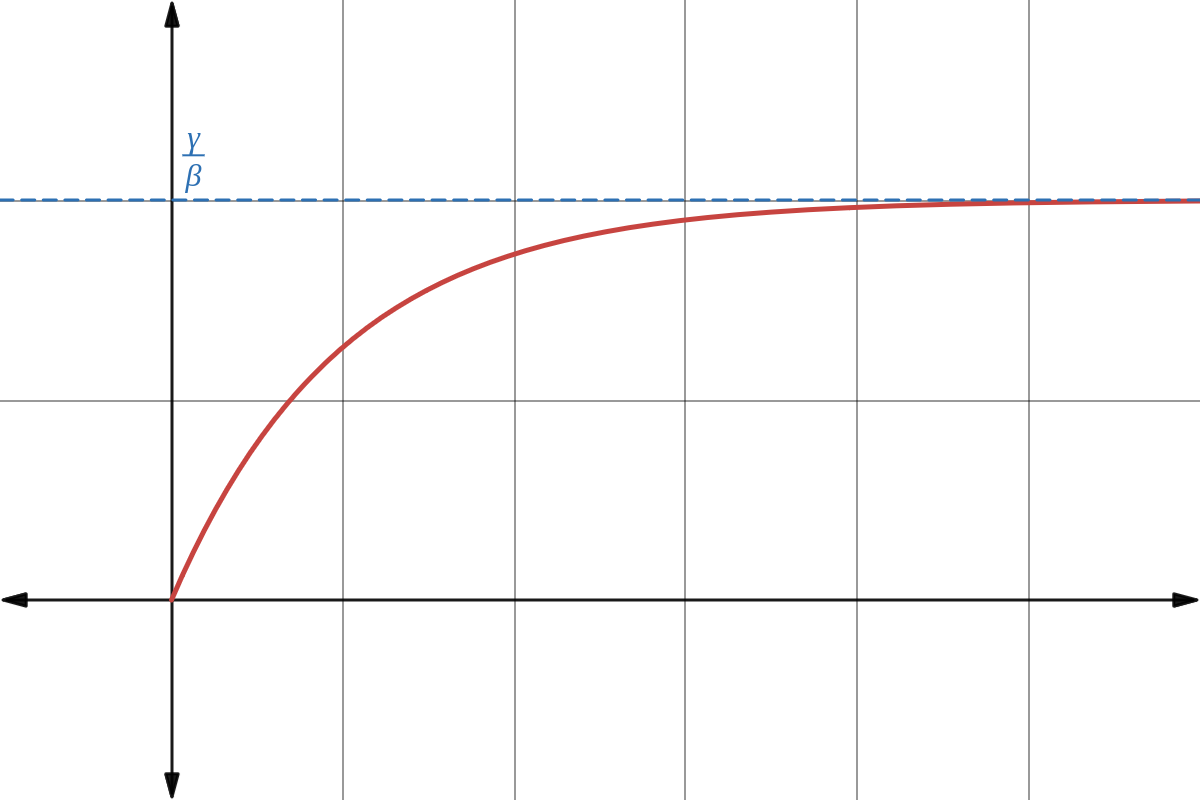
\includegraphics[scale=0.28]{../figures/crociera_first_order.png}
\end{center}
\end{minipage}

\subsubsection{Poli del sistema ed equazione caratteristica}
Si ha che i \textbf{poli} del sistema in forma a variabili di stato sono un \textit{sottoinsieme} degli \textbf{autovalori} della matrice $A$, in quanto li troviamo come radici dell'equazione:
$$
p_1(s) = \det(sI - A)
$$
al denominatore dell'inversa di $sI - a$, che corrisponde al polinomio caratteristico di $A$:
$$
p_2(s) = \det(A - \lambda I)
$$

Diciamo \textit{sottoinsieme} in quanto potrebbe esserci semplificazione fra numeratore e denominatore della funzione di trasferimento.
Quindi, non tutti gli autovalori della matrice $A$ diventeranno poli della funzione di trasferimento.
In particolare, dalla definizione di raggiungbilità ed osservabilità che avevamo dato, abbiamo che per ogni funzione di trasferimento $g_{ij}(s)$, i poli della funzione di trasferimento sono tutti e soli i poli (modi) raggiungibili dall'ingresso $u_j$ ed osservabili dall'uscita $y_i$.

Questo discorso tornerà utile quando discuteremo la differenza fra stabilità e \textit{BIBO} stabilità.

\subsection{Stabilità nel modello a funzione di trasferimento}
Abbiamo lavorato finora col modello a funzione di trasferimento, definita come:
$$
G(s) = \frac{\sum_{i = 0}^m b_i s^i}{\sum_{i = 0}^n a_i s^i} = \frac{ b_m (s - z_1) (s - z_2) ... (s - z_m) }{ a_n (s - p_1) (s - p_2) ... (s - p_n) }
$$
con $z_i$ gli $m$ \textit{zeri}, $p_i$ gli $n$ \textit{poli}, e $n > m$.

Di questa avevamo individuato le due forme:
\begin{itemize}
	\item \textbf{Forma di Evans:} evidenzia poli e zeri:
		$$
G(s) = \frac{\sum_{i = 0}^m b_i s^i}{\sum_{i = 0}^n a_i s^i} = \frac{ b_m (s - z_1) (s - z_2) ... (s - z_m) }{ a_n (s - p_1) (s - p_2) ... (s - p_n) }
		$$
	\item \textbf{Forma di Bode:} evidenzia le costanti tempo: 
		$$
G(s) = K \frac{ (\tau_a s + 1) (\tau_b s + 1) ... (\tau_i s + 1) }{ (\tau_1 s + 1) (\tau_2 s + 1) ... (\tau_n s + 1) }
		$$
\end{itemize}

Definiamo quindi formalmente \textbf{poli}:
\begin{definition}{Polo}
	Un polo $a_i$ di una funzione di trasferimento $G(s)$ è un valore di $s$ per cui $G(s)$ tende ad infinito:
	$$
	F(s) = \frac{g(s)}{\prod_{i = 1}^x (s - a_i)^n_i}
	$$
	con $n_i$ ordine del polo.
\end{definition}
e \textbf{zeri}:
\begin{definition}{Zeri}
	Uno zero $a_i$ di una funzione di trasferimento $G(s)$ è un valore di $s$ per cui $G(s)$ tende a zero: 
	$$
	F(s) = \frac{\prod_{i = 1}^x (s - a_i)^m_i}{g(s)}
	$$
	con $m_i$ ordine dello zero.
\end{definition}

Quello che ci interesserà nella valutazione della \textbf{stabilità} dei sistemi sarà la posizione dei poli nel piano complesso.
In particolare, come avevamo detto per i modi nel modello a variabili di stato, poli a componente \textit{reale negativa} danno \textbf{stabilità asintotica}, poli a componente \textit{reale nulla} danno \textbf{stabilità marginale}, e poli a componente \textit{reale positiva} dano \textbf{instabilità}.
Inoltre la componente \textit{complessa} dà informazioni sull'oscillazione del sistema, con \textbf{oscillazioni smorzate} a componente \textit{complessa e reale non nulle}, e \textbf{oscillazioni continue} a componente \textit{reale nulla}.

Gli zeri, invece, non hanno effetto sulla stabilità.
Gli zeri a parte reale positiva hanno invece l'effetto di \textit{invertire} la risposta al gradino, almeno sul breve termine.

\subsubsection{Stabilità e autovalori}
Avevamo che si poteva passare da modello a variabili di stato a funzione di trasferimento come:
$$
G(s) = \frac{Y(s)}{U(s)} = C(sI - A)^{-1} B + D = \frac{n(s)}{d(s)}
$$

Chiaramente, $n(s)$ e $d(s)$ saranno i polinomi di cui ci interessavamo per il calcolo di poli e zeri, di cui abbiamo detto ad interessarci per la stabilità erano i soli poli.
Ora, visto che abbiamo detto che c'è una qualche corrispondenza fra poli e autovalori, avremo che si può controllare la stabilità dai soli autovalori della matrice $A$.
Questo è infatti esattamente quello che avevamo fatto nel modello a variabili di stato.

\subsubsection{Stabilità BIBO}
Per parlare propriamente di stabilità, in relazione all'ingresso, nei modelli a funzione di trasferimento, introduciamo la nozione di sistema \textbf{BIBO} \textit{Bounded Input, Bounded Output}:
\begin{definition}{Sistema BIBO}
	Un sistema si dice stabile BIBO se ad ogni ingresso limitato corrisponde un'uscita limitata.
\end{definition}

Si ha che, per sistemi lineari, la stabilità BIBO si ha se e solo se i poli della funzione di trasferimento hanno tutti parte reale $< 0$.
Notiamo che la stabilità BIBO, al confronto della stabilità semplice che avevamo valutato finora, non dipende soltanto dallo stato interno del sistema, ma dalla \textbf{risposta forzata}.

\subsubsection{Poli dominanti}
In un sistema BIBO stabile, quindi, i modi sono tutti segnali esponenzialmente smorzati.
Al di là del transitorio iniziale, in questa situazione si avrà che il comportamento prevalente del sistema è quello dei modi più lenti, cioè quelli più vicini all'asse immaginario.

\subsubsection{Riassunto sulla stabilità}
Abbiamo quindi che \textbf{stabilità interna} (quella che avevamo visto nei modelli a variabili di stato) e \textbf{BIBO stabilità} di un sistema sono caratteristiche legate fra di loro ma separate:
\begin{table}[h!]
	\center \rowcolors{2}{white}{black!10}
	\begin{tabular} { c || p{5cm} | p{5cm} }
	& \bfseries Stabilità interna & \bfseries BIBO stabilità \\ 
	\hline 
		\bfseries Derivazione & Dagli autovalori (modi) della matrice $A$. & Dai poli della funzione di trasferimento, \\ 
		\bfseries Comportamento & Comportamento naturale, a partire dalle condizioni iniziali. & Sottoposto a un ingresso (risposta forzata) $u$ variabile $\neq 0$.
	\end{tabular}
\end{table}

La stabilità interna implica solitamente la stabilità BIBO, ma questo potrebbe non essere il caso se ci sono cancellazioni.
Possono esistere infatti esempi di sistemi BIBO stabili ma non internamente stabili, e viceversa.

Nel primo caso, il sistema potrebbe sembrare stabile "agli effetti esterni", ma determinate eccitazioni potrebbero portare a comportamenti instabili (oscillazioni incontrollate, ecc...), che solitamente raggiungono stati fisicamente 
impossibili all'interno del sistema stesso, e quindi fallimento.

Nel secondo, si potrebbero avere sistemi "di per sé" stabili, ma che rispondono in maniera negativa anche a piccolissime sollecitazioni esterne, rendendoli effettivamente instabili dal punto di vista della dinamica agli effetti esterni.

\subsection{Stabilità di sistemi in circuito chiuso}
Avevamo detto che i poli del sistema sono quelli che decidono la stabilità di un sistema.

\noindent
\begin{minipage}{\textwidth}
Preso ad esempio il sistema in ciclo chiuso:

\begin{center}
	\begin{tikzpicture}
		\draw (1,0) rectangle (3, 1);
		\node at (2, 0.5) {$G(s)$};
		
		\draw (-3,0) rectangle (-1, 1);
		\node at (-2, 0.5) {$C(s)$};

		\draw (-1.5, -0.5) rectangle (0.5, -1.5);
		\node at (-0.5, -1) {$H(s)$};

		\draw[-stealth] (-7, 0.5) -> (-5.1, 0.5);
		\draw[-stealth] (-5, 0.5) -> (-3, 0.5);
		\draw[-stealth] (-1, 0.5) -> (1, 0.5);
		\draw[-stealth] (3, 0.5) -> (3.9, 0.5);
		\draw[-stealth] (4, 0.5) -> (7, 0.5);
		
		\draw (5, 0.5) -> (5, -1);
		\draw[-stealth] (5, -1) -> (0.5, -1);
		\draw (-1.5, -1) -> (-5, -1);
		\draw[-stealth] (-5, -1) -> (-5, 0.5);

		\draw[-stealth] (4, 1.5) -> (4, 0.6);
		\node at (4, 1.75) {disturbo};

		\draw[fill=white] (-5, 0.5) circle (0.1);
		\draw[fill=white] (4, 0.5) circle (0.1);

		\node at (-6, 0.75) {$R(s)$};
		\node at (6, 0.75) {$Y(s)$};

		\node at (-4.75, 0.75) {$+$};
		\node at (-4.75, 0.25) {$-$};

		\node at (-3.8, 0.75) {\textit{errore}};
		\node at (0, 0.75) {\textit{controllo}};
		\node at (-3.5, -1.5) {\textit{feedback}};
	\end{tikzpicture}
\end{center}
\end{minipage}

\par\medskip

Dove le funzioni $C(s)$, $G(s)$ e $H(s)$ rappresentano rispettivamente il \textbf{controllore}, l'\textbf{impianto} e il \textbf{sensore}.
La funzione di trasferimento, trascurati i disturbi, avevamo detto era:
$$
\frac{Y(s)}{R(s)} = T(s) = \frac{C(s) G(s)}{1 + C(s)G(s)H(s)}
$$
da cui la stabilità del sistema è data dalla catena di retroazione completa (denominatore $d(s) = 1 + C(s)G(s)H(s))$, mentre la catena diretta $n(s) = C(s)G(s)$ dà solo gli zeri.

Del sistema in catena chiusa, quindi, valuteremo la stabilità controllando se i \textit{poli}  si trovano nella cosiddettà \textbf{regione di stabilità}, individuata come l'insieme di $z$ sul piano complesso a $\mathrm{Re}(z) < 0$.

Possiamo generalizzare il seguente discorso prendendo due funzioni di trasferimento, dette $G_{OL}$ (\textit{Open Loop}, in \textbf{anello aperto}), e $G_{CL}$ (\textit{Closed Loop}, in \textbf{anello chiuso}).
A questo punto potremo definire la funzione di trasferimento come:
$$
\frac{Y(s)}{R(s)} = T(s) = \frac{G_{OL}(s)}{1 + G_{CL}(s)}
$$
Notiamo che $G_{CL}$ è quanto si rileva dall'uscita attraverso il sensore, cioè:
$$
G_{CL}(s) = G_{OL}(s) H(s)
$$
e se $H(s) = 1$, la funzione di trasferimento sarà:
$$
\frac{Y(s)}{R(s)} = T(s) = \frac{G_{OL}(s)}{1 + G_{OL}(s)} \quad (H(s) = 1)
$$
Notiamo nuovamente che sarà solo il denominatore, in entrambi i casi, ad importarci per quanto riguarda la stabilità.

Facciamo alcuni esempi.

\subsubsection{Esempio: stabilità in catena chiusa}
Prendiamo il sistema con funzione di trasferimento in catena aperta:
$$
G_{OL} = \frac{10(0.5s + 1)}{s(2s + 1)}
$$
e trasferimento del sensore all'unità, e consideriamone la BIBO stabilità.
Vorremo prendere il solo denominatore:
$$
d(s) = 1 + G_{OL} = \frac{s(2s + 1) + 10(0.5s + 1)}{s(2s + 1)}
$$
di cui ci interessano solo gli zeri (cioè i poli di $T(s)$ funzione di trasferimento complessiva del sistema), quindi il numeratore::
$$
n'(s) = 2s^2 + s + 5s +10 = 2s^2 + 3s + 10
$$
di cui gli zeri:
$$
p_{1, 2} = \frac{-3}{4} \pm i \frac{\sqrt{79}}{4}
$$
con parte reale $< 0$, quindi il sistema è BIBO stabile.

\subsubsection{Esempio: stabilità in catena chiusa con parametro}
Prendiamo adesso un sistema con trasferimento in catena aperta determinato da un parametro:
$$
G_{OL} = s + 0.2 k - 2
$$
con transferimento del sensore sempre all'unità.
La domanda potrebbe essere per quali valori di $k$ il sistema è stabile.
Prendiamo allora il denominatore:
$$
d(s) = 1 + G_{OL} = s + 0.2 k - 1 \implies s = 1 - 0.2k
$$
di cui vediamo, se vogliamo poli in $s < 0$ e assumiamo $k \in \mathbb{R}$, dobbiamo imporre la condizione:
$$
k < 5
$$

\subsubsection{Esempio: stabilità in catena chiusa con parametro al second'ordine}
Facciamo un esempio analogo al precedente ma con una funzione di trasferimento del secondo grado:
$$
G_{OL} = \frac{k}{(2s + 1)(5s + 1)}
$$
con gli stessi assunti di prima sul sensore.
In questo caso il denominatore sarà:
$$
1 + G_{OL} = 1 + \frac{k}{(2s + 1)(5s + 1)} = \frac{10s^ + 7s  k + 1}{(2s + 1)(5s + 1)}
$$
da cui il numeratore:
$$
n'(s) = 10s^2 + 7s + k + 1
$$
per imporre $s < 0$, in questo caso, si dovrà dire:
$$
p_{1, 2} = \frac{-7 \pm \sqrt{49 - 40 (k + 1)}}{2(k + 1)}
$$
quindi parti reali:
$$
\mathrm{Re}(p_{1,2}) = -\frac{7}{2(k + 1)}
$$
e $k < -1$.

\subsection{Criterio di Routh}
Il \textbf{criterio di Routh} (\textit{criterio di Routh-Hurwitz}) è il primo metodo che vediamo per sistematizzare il procedimento di valutazione della stabilità.
Rappresenta un metodo \textit{puramente algebrico} che si applica a sistemi di controllo lineari tempo invarianti (\textit{LTI}).

Di base abbiamo che considereremo equazioni caratteristiche in forma polinomiale:
$$
p(s) = a_n s^n + a_{n - 1}s^{n - 1} + ... + a_1 s + a_0 = 0
$$
ciò che ci interessa è capire, guardando solo ai coefficienti $a_n, ..., a_0$, il segno delle componenti reali delle radici del polinomio, e in particolare sapere se queste sono tutte negative.
Il criterio di Routh ci permette di fare esattamente questo.

Vediamo innanzitutto le \textbf{condizioni di applicabilità}.
Abiamo la condizione necessaria ma non sufficiente per la stabilità, che tutti gli $n + 1$ coefficienti del polinomio devono avere lo stesso segno.
Questa è fra l'altro necessaria e sufficiente per $n \leq 2$.

Vorremo quindi calcolare la cosiddetta \textbf{tabella di Routh}.
Per un polinomio di grado $n$, questa avrà $n + 1$ righe.
Le prime due righe sono sempre costituite dai coefficienti del polinomio $p(s)$, distinto in una parte pari e una parte dispari.
Cioè assunto $n$ pari:
\[
	\begin{cases}
		p_1(s) = a_n s^N + a_{n - 2} s^{n - 2} + ... + a_0 \quad \hspace{0.85cm} \text{(pari)} \\
		p_2(s) = a_{n - 1} s^{n - 1} + a_{n - 3} s^{n - 3} + ... + a_1 s \quad \text{(dispari)}
	\end{cases}
\]

Potremo quindi dire:
\begin{table}[h!]
	\center 
	\begin{tabular} { c | c c c c }
		$n$ & $a_n$ & $a_{n - 2}$ & $a_{n - 4}$ & ... \\
		$n - 1$ & $a_{n - 1}$ & $a_{n - 3}$ & $a_{n - 5}$ & ... \\
		$n - 2$ & $b_1$ & $b_2$ & $b_3$ & ... \\
		$\vdots$ & ... & ... & ... \\
		1 & $y_1$ & $y_2$ \\
		0 & $z_1$
	\end{tabular}
\end{table}

Per i termini successivi si prende, ad esempio alla terza riga:
$$
b_1 = - \frac{ \det \begin{pmatrix}
	a_n & a_{n - 2} \\
	a_{n - 1} & a_{n - 3}
\end{pmatrix} }{a_{n - 1}}, \quad
b_2 = - \frac{ \det \begin{pmatrix}
	a_n & a_{n - 4} \\
	a_{n - 1} & a_{n - 5}
\end{pmatrix} }{a_{n - 1}}, \quad ...
$$
e cosi via per righe successive, cioè ogni volta si prende il minore ottenuto prendendo le due righe alla prima colonna  alla $i + 1$-esima dove $i$ è la colonna che consideriamo.
Vediamo che questo procedimento riduce automaticamente il numero di colonne di $1$ ogni $2$ righe (per gli elementi che rimangono \textit{a metà}, cioe non sono definiti sulla riga corrente, si prende 0).

Sulla tabella di Routh si possono dimostrare 2 teoremi, il primo riguardo alla condizione che cercavamo:
\begin{theorem}{Primo teorema di Routh}
	Condizione necessaria e sufficiente perchè tutte le radici dell'equazione caratteristica abbiano parte reale negativa è che tutti gli elementi della prima colonna della tabella di Routh siano positivi e non nulli.
\end{theorem}
e il secondo nel caso il primo fallisse:
\begin{theorem}{Secondo teorema di Routh}
	Se qualche elemento della prima colonna è negativo, il numero di radici con parte reale positiva è uguale al numero di cambi di segno dei coefficienti della prima colonna.
\end{theorem}

\end{document}


\documentclass[a4paper,11pt]{article}
\usepackage[a4paper, margin=8em]{geometry}

% usa i pacchetti per la scrittura in italiano
\usepackage[french,italian]{babel}
\usepackage[T1]{fontenc}
\usepackage[utf8]{inputenc}
\frenchspacing 

% usa i pacchetti per la formattazione matematica
\usepackage{amsmath, amssymb, amsthm, amsfonts}

% usa altri pacchetti
\usepackage{gensymb}
\usepackage{hyperref}
\usepackage{standalone}

% imposta il titolo
\title{Appunti Fondamenti di Automatica}
\author{Luca Seggiani}
\date{2025}

% disegni
\usepackage{pgfplots}
\pgfplotsset{width=10cm,compat=1.9}

% imposta lo stile
% usa helvetica
\usepackage[scaled]{helvet}
% usa palatino
\usepackage{palatino}
% usa un font monospazio guardabile
\usepackage{lmodern}

% tikz in sans
\tikzset{every picture/.style={/utils/exec={\sffamily}}}

\renewcommand{\rmdefault}{ppl}
\renewcommand{\sfdefault}{phv}
\renewcommand{\ttdefault}{lmtt}

% circuiti
\usepackage{circuitikz}
\usetikzlibrary{babel}

% disponi il titolo
\makeatletter
\renewcommand{\maketitle} {
	\begin{center} 
		\begin{minipage}[t]{.8\textwidth}
			\textsf{\huge\bfseries \@title} 
		\end{minipage}%
		\begin{minipage}[t]{.2\textwidth}
			\raggedleft \vspace{-1.65em}
			\textsf{\small \@author} \vfill
			\textsf{\small \@date}
		\end{minipage}
		\par
	\end{center}

	\thispagestyle{empty}
	\pagestyle{fancy}
}
\makeatother

% disponi teoremi
\usepackage{tcolorbox}
\newtcolorbox[auto counter, number within=section]{theorem}[2][]{%
	colback=blue!10, 
	colframe=blue!40!black, 
	sharp corners=northwest,
	fonttitle=\sffamily\bfseries, 
	title=Teorema~\thetcbcounter: #2, 
	#1
}

% disponi definizioni
\newtcolorbox[auto counter, number within=section]{definition}[2][]{%
	colback=red!10,
	colframe=red!40!black,
	sharp corners=northwest,
	fonttitle=\sffamily\bfseries,
	title=Definizione~\thetcbcounter: #2,
	#1
}

% disponi problemi
\newtcolorbox[auto counter, number within=section]{problem}[2][]{%
	colback=green!10,
	colframe=green!40!black,
	sharp corners=northwest,
	fonttitle=\sffamily\bfseries,
	title=Problema~\thetcbcounter: #2,
	#1
}

% disponi codice
\usepackage{listings}
\usepackage[table]{xcolor}

\lstdefinestyle{codestyle}{
		backgroundcolor=\color{black!5}, 
		commentstyle=\color{codegreen},
		keywordstyle=\bfseries\color{magenta},
		numberstyle=\sffamily\tiny\color{black!60},
		stringstyle=\color{green!50!black},
		basicstyle=\ttfamily\footnotesize,
		breakatwhitespace=false,         
		breaklines=true,                 
		captionpos=b,                    
		keepspaces=true,                 
		numbers=left,                    
		numbersep=5pt,                  
		showspaces=false,                
		showstringspaces=false,
		showtabs=false,                  
		tabsize=2
}

\lstdefinestyle{shellstyle}{
		backgroundcolor=\color{black!5}, 
		basicstyle=\ttfamily\footnotesize\color{black}, 
		commentstyle=\color{black}, 
		keywordstyle=\color{black},
		numberstyle=\color{black!5},
		stringstyle=\color{black}, 
		showspaces=false,
		showstringspaces=false, 
		showtabs=false, 
		tabsize=2, 
		numbers=none, 
		breaklines=true
}

\lstdefinelanguage{javascript}{
	keywords={typeof, new, true, false, catch, function, return, null, catch, switch, var, if, in, while, do, else, case, break},
	keywordstyle=\color{blue}\bfseries,
	ndkeywords={class, export, boolean, throw, implements, import, this},
	ndkeywordstyle=\color{darkgray}\bfseries,
	identifierstyle=\color{black},
	sensitive=false,
	comment=[l]{//},
	morecomment=[s]{/*}{*/},
	commentstyle=\color{purple}\ttfamily,
	stringstyle=\color{red}\ttfamily,
	morestring=[b]',
	morestring=[b]"
}

% disponi sezioni
\usepackage{titlesec}

\titleformat{\section}
	{\sffamily\Large\bfseries} 
	{\thesection}{1em}{} 
\titleformat{\subsection}
	{\sffamily\large\bfseries}   
	{\thesubsection}{1em}{} 
\titleformat{\subsubsection}
	{\sffamily\normalsize\bfseries} 
	{\thesubsubsection}{1em}{}

% disponi alberi
\usepackage{forest}

\forestset{
	rectstyle/.style={
		for tree={rectangle,draw,font=\large\sffamily}
	},
	roundstyle/.style={
		for tree={circle,draw,font=\large}
	}
}

% disponi algoritmi
\usepackage{algorithm}
\usepackage{algorithmic}
\makeatletter
\renewcommand{\ALG@name}{Algoritmo}
\makeatother

% disponi numeri di pagina
\usepackage{fancyhdr}
\fancyhf{} 
\fancyfoot[L]{\sffamily{\thepage}}

\makeatletter
\fancyhead[L]{\raisebox{1ex}[0pt][0pt]{\sffamily{\@title \ \@date}}} 
\fancyhead[R]{\raisebox{1ex}[0pt][0pt]{\sffamily{\@author}}}
\makeatother

\begin{document}

% sezione (data)
\section{Lezione del 08-04-25}

% stili pagina
\thispagestyle{empty}
\pagestyle{fancy}

% testo
Ritorniamo sul criterio di Routh.

\subsubsection{Criterio di Routh simbolico}
Il criterio di Routh torna particolarmente utile quando il polinomio studiato ha un coefficiente simbolico.
Ad esempio prendiamo la funzione di trasferimento in ciclo aperto:
$$
G_{OL} = \frac{K_c}{(s + 1)(\frac{s}{2} + 1)(\frac{s}{3} + 1)}
$$
I poli del ciclo aperto sono banali in quanto il polinomio al denominatore è gia fattorizzato ($p_{1,2,3} = 1,2,3$).
Calcoliamo allora i poli al denominatore della retroazione:
$$
1 + G_{OL} = 1 + \frac{K_c}{(s + 1)(\frac{s}{2} + 1)(\frac{s}{3} + 1)} = 
\frac{ s^3 + 6 s^2 + 11s + 6 ( 1 + K_c ) }{ (s + 1)(\frac{s}{2} + 1)(\frac{s}{3} + 1) } 
$$
Come notiamo, compare il parametro $K_c$ al termine noto.
Applichiamo allora il criterio di Routh:
$$
\begin{array}{c | c c}
		3 & 1 & 11 \\
		2 & 6 & 6(1 + K_c) \\
		1 & 10 - K_c \\
		0 & 6(1 + K_c)
\end{array}
$$
Vorremo quindi impostare il sistema:
\[
	\begin{cases}
		10 - K_c > 0 \\
		6(1 + K_c) > 0
	\end{cases}
\]
da cui $-1 < K_c < 10$ è il range in cui il polinomio non ha radici positive.

\par\medskip

\noindent
\begin{minipage}{\textwidth}
Vediamo che quello che abbiamo fatto è effettivamente prendere il sistema:

\begin{center}
	\begin{tikzpicture}
		\draw (1,0) rectangle (3, 1);
		\node at (2, 0.5) {$G(s)$};
		
		\draw (-3,0) rectangle (-1, 1);
		\node at (-2, 0.5) {$K_c$};

		\draw (-1.5, -0.5) rectangle (0.5, -1.5);
		\node at (-0.5, -1) {$H(s) = 1$};

		\draw[-stealth] (-7, 0.5) -> (-5.1, 0.5);
		\draw[-stealth] (-5, 0.5) -> (-3, 0.5);
		\draw[-stealth] (-1, 0.5) -> (1, 0.5);
		\draw[-stealth] (3, 0.5) -> (7, 0.5);
		
		\draw (5, 0.5) -> (5, -1);
		\draw[-stealth] (5, -1) -> (0.5, -1);
		\draw (-1.5, -1) -> (-5, -1);
		\draw[-stealth] (-5, -1) -> (-5, 0.5);

		\draw[fill=white] (-5, 0.5) circle (0.1);


		\node at (-4.75, 0.75) {$+$};
		\node at (-4.75, 0.25) {$-$};

	\end{tikzpicture}
\end{center}
\end{minipage}

\par\medskip
\noindent
a sensore unitario, con la $G(s)$:
$$
G(s) = \frac{G_{OL}}{K_c} = \frac{1}{(s + 1)(\frac{s}{2} + 1)(\frac{s}{3} + 1)}
$$
e tarare il componente $K_c$, che chiamiamo \textit{proporzionale}, in modo da arrivare alla stabilità del sistema.

\subsubsection{Casi singolari del criterio di Routh}
Vediamo alcuni casi particolari del criterio di Routh.
\begin{itemize}
\item \textbf{Primo termine di una riga nullo:} in questo caso il problema sarà che è nullo il pivot per la costruzione della nuova tabella, e ci troveremmo a dividere per zero.
In questo caso possiamo sostituire gli 0 con $\epsilon$ piccoli a piacere.
Portiamo quindi avanti i calcoli conservando zero, e calcolando i termini successivi prendendo il limite $\epsilon \rightarrow 0^+$.
Ad esempio:
$$
\begin{array}{c | c c}
	3 & 1 & 1 \\
	2 & 0 & 2
\end{array}
$$
diventa:
$$
\begin{array}{c | c c}
	3 & 1 & 1 \\
	2 & \epsilon & 2 \\
	1 & \frac{\epsilon - 2}{\epsilon} & 0 \\
	0 & 2
\end{array}
$$
da cui la prima colonna, preso il limite, sarà:
$$
\begin{array}{c | c}
	3 & 1 \\
	2 & 0^+ \\
	1 & - \infty \\
	0 & 2
\end{array}
$$
con un cambiamento di segno e quindi una radice reale positiva.

\noindent
\begin{minipage}{\textwidth}
Abbiamo infatti che il polinomio sul piano complesso ha il seguente aspetto:
\begin{center}
	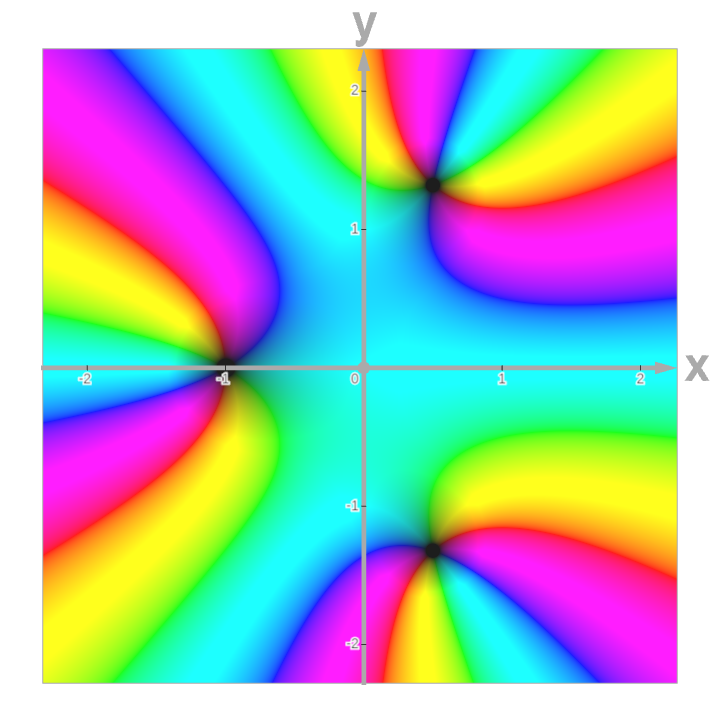
\includegraphics[scale=0.3]{../figures/polynomial_routh_1.png}
\end{center}
\end{minipage}

\par\medskip

da cui notiamo il polo stabile in $p_1 = -1$, e i poli complessi coniugati instabili in $p_{2,3} = \frac{1}{2} \pm \frac{\sqrt{7}}{2}$ (che troviamo anche fattorizzando in $(x + 1) (x^2 - x + 2)$).

\item \textbf{Intera riga nulla:} partiamo dall'esempio del polinomio:
$$
\rho(s) = s^3 + bs^2 + cs + 1
$$
da cui:
$$
\begin{array}{c | c c}
	3 & 1 & c \\
	2 & b & 1 \\
	1 & \frac{bc - 1}{b} \\
	0 & 1
\end{array}
$$
Nel caso $bc = 1$, tutta la riga 1 è nulla.
Questo può essere problematico per la valutazione della stabilità: diciamo allora che con $b, c > 0$, e $bc > 1$, si ha che il polinomio ha solo radici stabili dal primo teorema di Routh.

Per il caso $bc = 1$, invece, possiamo usare più metodi:
\begin{itemize}
	\item Possiamo usare il cosiddetto \textbf{metodo dell'equazione ausiliaria}.
Consideriamo quindi la riga immediatamente superiore a quella nulla:
$$
bs^2 + 1 = 0 \rightarrow s^*_{1, 2} = \pm j \sqrt{ \frac{1}{b} }
$$
avremo che le radici di tale equazione coincidono con le radici mancanti per le quali la tabella non aveva dato soluzioni.
In questo caso, le radici sono complesse coniugate oscillanti, e siamo quindi in condizioni di stabilità.

	\item Il problema del metodo dell'equazione ausiliaria è che ci richiede di risolvere un nuovo polinomio, che nello scorso esempio era semplice (grado 2), ma ptorebbe non esserlo in un caso reale.
Introduciamo quindi il \textbf{metodo della derivata}: prendiamo la derivata rispetto ad $s$ dell'ultima riga e sostituiamo i coefficienti alla riga tutta nulla, cioè scriviamo:
$$
\frac{d}{ds} \left( bs^2 + 1 \right) = 2bs
$$
e quindi sostituiamo:
$$
\begin{array}{c | c c}
	3 & 1 & c \\
	2 & b & 1 \\
	1 & 2b \\
	0 & 1
\end{array}
$$
In questo caso, se la prima colonna modificata non presentà variazioni di segno (è stabile), si ha \textit{stabilità semplice}, mentre se si hanno variazioni di segno abbiamo instabilità per la presenza di poli reali positivi, o poli immaginari con molteplicità $> 1$.

Nell'esempio particolare, abbiamo che con $b<0$ il sistema è instabile, ma ce ne potevamo già accorgere dal fatto che $b<0$ viola le condizioni di applicabilità di Routh.
\end{itemize}

In verità, righe nulle nella matrice di Routh possono derivare solo da casi di \textbf{simmetria quadrantale} delle radici, cioè radici simmetriche rispetto all'asse reale e all'asse immaginario.
Da questa considerazione derivano i criteri precedenti.

Un'ultima considerazione è che, quando si incontrano configurazioni polari con soluzioni immaginarie pure, quello che si trova sono effettivamente le frequenze di oscillazione del sistema, cioè quelle ai limiti della stabilità per cui il sistema dinamico oscilla.
Nel caso precedente avevamo ad esempio trovato che questa era $\omega = \sqrt{\frac{1}{b}}$, dalla coppia di radici complesse coniugate $s^*_{1, 2} = \pm j \sqrt{ \frac{1}{b} }$

\end{itemize}

\subsection{Risposta in frequenza}
Iniziamo quindi a parlare della \textbf{risposta in frequenza} dei sistemi, in particolare con riferimento ai \textit{diagrammi di Bode}.

La risposta in frequenza, detta anche \textit{risposta armonica}, è una proprieta dei sistemi lineari asintoticamente stabili, cioè con poli oscillanti a molteplicità 1 o poli reali non positivi.

\noindent
\begin{minipage}{\textwidth}
I risultati che otterremo si basano sul \textbf{teorema della risposta armonica}:
\begin{theorem}{Teorema della risposta armonica}
Ad un sistema con funzione di trasferimento $G(s)$:
\begin{center}
	\begin{tikzpicture}
		\draw (0,0) rectangle (2, 1);
		\draw[-stealth] (-2, 0.5) -> (0, 0.5);
		\draw[-stealth] (2, 0.5) -> (4, 0.5);
		\node at (1, 0.5) {$G(s)$};
		\node at (-1, 0.7) {$U(s)$};
		\node at (3, 0.7) {$Y(s)$};
	\end{tikzpicture}
\end{center}
se applichiamo un segnale di ingresso sinusoidale:
$$
u(t) = U_M \sin(\omega t)
$$
esaurito il transitorio, l'uscita sarà ancora sinusoidale:
$$
y(t) = |Y(\omega)| \sin\left(\omega t + \phi(\omega)\right)
$$
con pulsazione e fase della sinusoide d'uscita determinati dalla pulsazione della sinusoide di ingresso.
\end{theorem}
\end{minipage}

\par\medskip

Lo scopo dei diagrammi di Bode, vediamo, sarà valutare $Y(\omega)$ e $\phi(\omega)$ al variare della pulsazione $\omega$, o meglio per tutte le pulsazioni $\omega$.

Dimostriamo innanzitutto che una funzione di trasferimento $G(s)$ sottoposta a uno stimolo sinusoidale dà una risposta sinusoidale, cioè prendiamo:
$$
u(t) \sim \sin(\omega t) = \frac{1}{2j} \left( e^{j \omega t} - e^{-j \omega t} \right)
$$
$$
\implies \mathcal{L}\left\{u(t)\right\} = U(s) = \frac{1}{2j} \left( \frac{1}{s- j\omega} - \frac{1}{s + j\omega} \right) = \frac{\omega^2}{s^2 + \omega^2}
$$
L'uscita sarà quindi:
$$
Y(s) = G(s) U(s) = \frac{A_1}{s - j \omega} + \frac{A_1^*}{s + j \omega} + \text{transitori}
$$
vediamo che i transitori vanno a $0$ nel caso di sistemi stabili, in quanto sono in forma $e^{-pt}$ con $p$ positivo, per cui possiamo ignorarli sul lungo termine (come avevamo assunto per ipotesi nella definizione stessa di risposta in frequenza), quindi:
$$
Y(s) \Big|_{t \rightarrow +\infty} = \frac{A_1}{s - j \omega} + \frac{A_1^*}{s + j \omega}
$$
Calcoliamo quindi il residuo $A_1$, consci del fatto che l'altro coefficiente ($A_1^*$) ne sarà semplicemente il coniugato:
$$
A_1 = \lim_{s \rightarrow j \omega} (s - j \omega) G(s) U(s) = (s - j \omega) G(s) \frac{\omega}{(s - j \omega)(s + j \omega)} = G(j \omega) \frac{1}{2j}
$$
e quindi:
$$
A_1^* = -G(-j \omega) \frac{1}{2j}
$$
Troviamo allora la $Y(s)$ a infinito:
$$
Y(s) \Big|_{t \rightarrow +\infty} = \frac{G(j\omega)}{2j} e^{j \omega t} - \frac{G(- j\omega)}{2j} e^{-j \omega t}
$$
Usiamo una semplificazione, visto che la somma di due coniugi dà 2 volte la parte reale di entrambi, cioè:
$$
z + z^* = 2 \mathrm{Re}\left\{z\right\}, \quad \forall z \in \mathbb{C}
$$
e quindi:
$$
G(j \omega) = |G(j \omega)| e^{j \angle G(j \omega)}
$$
che applicando nuovamente la proprietà e sostituendo dà:
$$
Y(s) \Big|_{t \rightarrow +\infty} = 2 \mathrm{Re} \left\{ \frac{G(j \omega)}{2j} e^{j \omega t} \right\} = \mathrm{Re} \left\{ \frac{|G(j \omega)|}{j} e^{j(\omega t + \angle G(j \omega))} \right\}
$$
$$
= \mathrm{Re} \left\{ \frac{|G(\omega)|}{j} \cos(\omega t + \angle G(j \omega)) + |G(j \omega)| \sin(\omega t + \angle G(j \omega)) \right\}
$$
$$
=|G(j \omega)| \sin(\omega t + \angle G(j \omega))
$$
che è esattamente l'ipotesi. \qed

\par\smallskip

Il procedimenti che adotteremo, quindi, è quello di modellare un sistema (che prendiamo come una \textit{scatola nera}) sulla base dalla sua \textit{risposta in frequenza}, magari sfruttando strumenti come l'\textbf{oscilloscopio}:

\begin{center}
	\begin{tikzpicture}
		\draw (0,0) rectangle (2, 1);
		\draw[-stealth] (-2, 0.5) -> (0, 0.5);
		\draw[-stealth] (2, 0.5) -> (4, 0.5);
		\node at (1, 0.5) {$G(s)$};
		\node at (-1, 0.7) {\sffamily{ingresso}};
		\node at (3, 0.7) {\sffamily{uscita}};

		\draw[-stealth] (-1, 0.5) -> (-1, -0.5);
		\draw[-stealth] (3, 0.5) -> (3, -0.5);
		
		\node at (-1, -0.8) {\sffamily{oscilloscopio}};
		\node at (3, -0.8) {\sffamily{oscilloscopio}};
		\node at (-1, -1.15) {\sffamily{di ingresso}};
		\node at (3, -1.15) {\sffamily{di uscita}};
	\end{tikzpicture}
\end{center}

che potrebbero dare misurazioni del tipo:

\begin{center}
	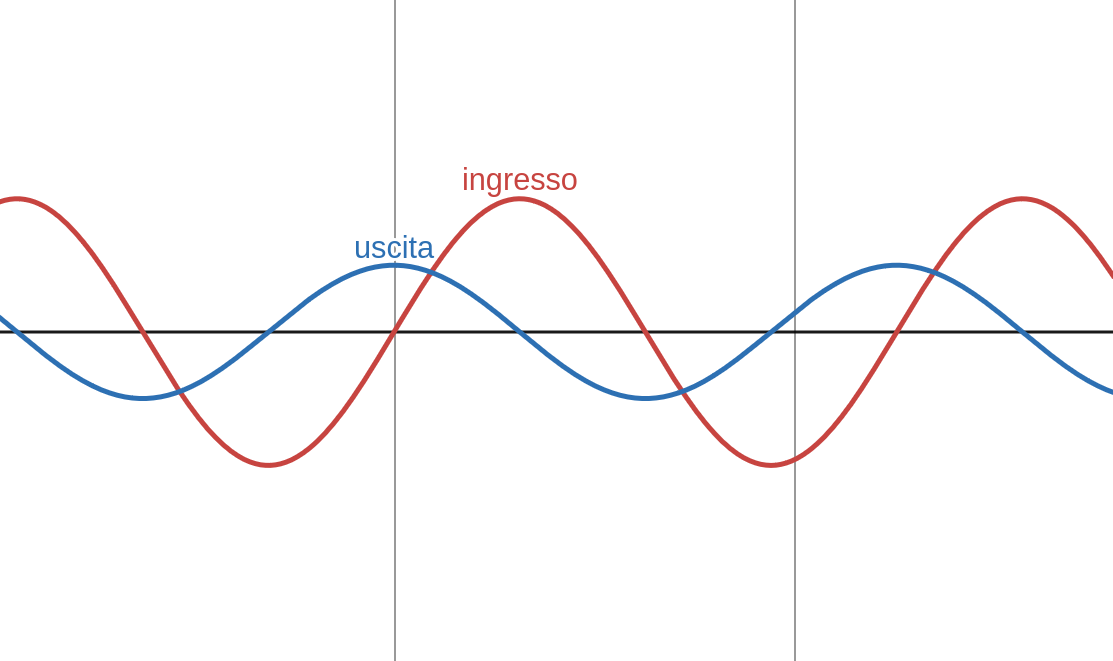
\includegraphics[scale=0.3]{../figures/in_out_sin.png}
\end{center}

Misurazioni di questo tipo evidenziano la variazione di ampiezza e lo scostamento in fase per segnali sinusoidali costanti in frequenza, e facendo più misurazioni per più frequenze si può avere un idea del trasferimento del sistema in dominio frequenze, cioè esattamente la risposta in frequenza.


\documentclass[a4paper,11pt]{article}
\usepackage[a4paper, margin=8em]{geometry}

% usa i pacchetti per la scrittura in italiano
\usepackage[french,italian]{babel}
\usepackage[T1]{fontenc}
\usepackage[utf8]{inputenc}
\frenchspacing 

% usa i pacchetti per la formattazione matematica
\usepackage{amsmath, amssymb, amsthm, amsfonts}

% usa altri pacchetti
\usepackage{gensymb}
\usepackage{hyperref}
\usepackage{standalone}

% imposta il titolo
\title{Appunti Fondamenti di Automatica}
\author{Luca Seggiani}
\date{2025}

% disegni
\usepackage{pgfplots}
\pgfplotsset{width=10cm,compat=1.9}

% imposta lo stile
% usa helvetica
\usepackage[scaled]{helvet}
% usa palatino
\usepackage{palatino}
% usa un font monospazio guardabile
\usepackage{lmodern}

% tikz in sans
\tikzset{every picture/.style={/utils/exec={\sffamily}}}

\renewcommand{\rmdefault}{ppl}
\renewcommand{\sfdefault}{phv}
\renewcommand{\ttdefault}{lmtt}

% circuiti
\usepackage{circuitikz}
\usetikzlibrary{babel}

% disponi il titolo
\makeatletter
\renewcommand{\maketitle} {
	\begin{center} 
		\begin{minipage}[t]{.8\textwidth}
			\textsf{\huge\bfseries \@title} 
		\end{minipage}%
		\begin{minipage}[t]{.2\textwidth}
			\raggedleft \vspace{-1.65em}
			\textsf{\small \@author} \vfill
			\textsf{\small \@date}
		\end{minipage}
		\par
	\end{center}

	\thispagestyle{empty}
	\pagestyle{fancy}
}
\makeatother

% disponi teoremi
\usepackage{tcolorbox}
\newtcolorbox[auto counter, number within=section]{theorem}[2][]{%
	colback=blue!10, 
	colframe=blue!40!black, 
	sharp corners=northwest,
	fonttitle=\sffamily\bfseries, 
	title=Teorema~\thetcbcounter: #2, 
	#1
}

% disponi definizioni
\newtcolorbox[auto counter, number within=section]{definition}[2][]{%
	colback=red!10,
	colframe=red!40!black,
	sharp corners=northwest,
	fonttitle=\sffamily\bfseries,
	title=Definizione~\thetcbcounter: #2,
	#1
}

% disponi problemi
\newtcolorbox[auto counter, number within=section]{problem}[2][]{%
	colback=green!10,
	colframe=green!40!black,
	sharp corners=northwest,
	fonttitle=\sffamily\bfseries,
	title=Problema~\thetcbcounter: #2,
	#1
}

% disponi codice
\usepackage{listings}
\usepackage[table]{xcolor}

\lstdefinestyle{codestyle}{
		backgroundcolor=\color{black!5}, 
		commentstyle=\color{codegreen},
		keywordstyle=\bfseries\color{magenta},
		numberstyle=\sffamily\tiny\color{black!60},
		stringstyle=\color{green!50!black},
		basicstyle=\ttfamily\footnotesize,
		breakatwhitespace=false,         
		breaklines=true,                 
		captionpos=b,                    
		keepspaces=true,                 
		numbers=left,                    
		numbersep=5pt,                  
		showspaces=false,                
		showstringspaces=false,
		showtabs=false,                  
		tabsize=2
}

\lstdefinestyle{shellstyle}{
		backgroundcolor=\color{black!5}, 
		basicstyle=\ttfamily\footnotesize\color{black}, 
		commentstyle=\color{black}, 
		keywordstyle=\color{black},
		numberstyle=\color{black!5},
		stringstyle=\color{black}, 
		showspaces=false,
		showstringspaces=false, 
		showtabs=false, 
		tabsize=2, 
		numbers=none, 
		breaklines=true
}

\lstdefinelanguage{javascript}{
	keywords={typeof, new, true, false, catch, function, return, null, catch, switch, var, if, in, while, do, else, case, break},
	keywordstyle=\color{blue}\bfseries,
	ndkeywords={class, export, boolean, throw, implements, import, this},
	ndkeywordstyle=\color{darkgray}\bfseries,
	identifierstyle=\color{black},
	sensitive=false,
	comment=[l]{//},
	morecomment=[s]{/*}{*/},
	commentstyle=\color{purple}\ttfamily,
	stringstyle=\color{red}\ttfamily,
	morestring=[b]',
	morestring=[b]"
}

% disponi sezioni
\usepackage{titlesec}

\titleformat{\section}
	{\sffamily\Large\bfseries} 
	{\thesection}{1em}{} 
\titleformat{\subsection}
	{\sffamily\large\bfseries}   
	{\thesubsection}{1em}{} 
\titleformat{\subsubsection}
	{\sffamily\normalsize\bfseries} 
	{\thesubsubsection}{1em}{}

% disponi alberi
\usepackage{forest}

\forestset{
	rectstyle/.style={
		for tree={rectangle,draw,font=\large\sffamily}
	},
	roundstyle/.style={
		for tree={circle,draw,font=\large}
	}
}

% disponi algoritmi
\usepackage{algorithm}
\usepackage{algorithmic}
\makeatletter
\renewcommand{\ALG@name}{Algoritmo}
\makeatother

% disponi numeri di pagina
\usepackage{fancyhdr}
\fancyhf{} 
\fancyfoot[L]{\sffamily{\thepage}}

\makeatletter
\fancyhead[L]{\raisebox{1ex}[0pt][0pt]{\sffamily{\@title \ \@date}}} 
\fancyhead[R]{\raisebox{1ex}[0pt][0pt]{\sffamily{\@author}}}
\makeatother

\begin{document}

% sezione (data)
\section{Lezione del 09-04-25}

% stili pagina
\thispagestyle{empty}
\pagestyle{fancy}

% testo
\subsection{Diagrammi di Bode}
I diagrammi di Bode sono 2:
\begin{enumerate}
	\item Il \textbf{diagramma di modulo} (o ampiezza): rappresenta il modulo di $G(j\omega)$ al variare della pulsazione $\omega$.
		Abbiamo quindi $|G(j \omega)|$ alle ordinate e $\omega$ alle ascisse, espresse in scala logaritmica.
		Il modulo si misura in deciBel (dB), già in scala logaritmica, mentre per la pulsazione $\omega$ si usa la scala logaritmica in base 10.
		Notiamo che il decibel è un \textbf{unità di misura relativa}: si interpreta come il rapporto fra due \textit{potenze}, espresso in scala logaritmica, dove per la seconda grandezza, detta \textbf{valore di riferimento}, assumiamo 1:
		$$
		\mathrm{dB} = 10 \cdot \log_{10} \left( \frac{P}{P_{ref}} \right) =  10 \cdot \log_{10} \left( \frac{P}{1} \right)
		$$
		Abbiamo quindi che il rapporto fra valore assoluto di ampiezza e il valore in decibel è:
		$$
		x_{dB} = 20 \log_{10}(|x|)
		$$

		Il 20 compare per via del fatto che consideriamo \textit{ampiezze}, mentre il decibel esprime rapporti fra \textit{potenze}.
	Abbiamo che la relazione fra ampiezza $A$ e potenza $P$ è quadratica:
	$$
	A^2 \propto P
	$$
	per cui si vuole calcolare effettivamente:
	$$
	\mathrm{dB} = 10 \cdot \log_{10} \left( \frac{P}{P_{ref}} \right) = 10 \cdot \log_{10} \left( \frac{A^2}{A_{ref}^2} \right) = 10 \cdot \log_{10} \left( \left( \frac{A}{A_{ref}} \right)^2 \right)
	$$
	$$
	= 10 \cdot 2 \cdot \log_{10} \left( \frac{A}{A_{ref}} \right) = 20 \cdot \log_{10} \left( \frac{A}{A_{ref}} \right)
	$$
	assunto $A_{ref} = 1$ come da ipotesi si ottiene la stessa formula di prima.

	\item Il \textbf{diagramma di fase:} rappresenta la fase di $G(j\omega)$ al variare della pulsazione $\omega$.
		Abbiamo quindi $\angle G(j \omega)$ alle ordinate e $\omega$ alle ascisse, la prima in scala lineare e la seconda nella stessa scala logaritmica in base 10 di prima.
\end{enumerate}

\subsubsection{Ascisse}
Abbiamo quindi che sulle \textbf{ascisse} abbiamo sempre la \textit{pulsazione}(rad/s) o \textit{frequenza} (Hz), che sono fra di loro direttamente proporzionali.
Queste sono espresse in scala logaritmica, e troviamo quindi i seguenti intervalli relativi:
\begin{itemize}
	\item \textbf{Decade:} è la distanza in scala logaritmica tra numeri il cui raporto è 10;
	\item \textbf{Ottava:} è la distanza in scala logartmica tra numeri il cui rapporto è 2.
\end{itemize}

\subsubsection{Ordinate}
Alle \textbf{ordinate} manteniamo invece, nel caso di un diagramma di modulo, lo spettro di ampiezza in unità logaritmiche (dB).
Abbiamo quindi che 0 dB equivalgono al valore di riferimento (1), mentre tutti gli altri valori si convertono usando la formula:
$$
\text{(decibel)} \quad 20 \log_{10}(10^\alpha) = 20 \cdot \alpha \quad \text{(scala logaritmica)}
$$

Nel caso di diagrammi di fase, invece, abiamo la fase in scala lineare, misurata in \textit{radianti} (rad) o in \textit{gradi} ($\circ$).

\par\medskip

Notiamo infine che il \textit{modulo} è una funzione \textbf{pari}:
$$
|G(j \omega)| = |G(-j \omega)|
$$
mentre la \textit{fase} è una funzione \textbf{dispari}:
$$
\angle G(j \omega) = - \angle G(-j \omega)
$$

\subsubsection{Proprietà dei diagrammi di Bode}
Abbiamo quindi che i diagrammi di Bode sono molto comodi per avere rappresentazioni dettagliat di grandezze che variano in campi notevolmente estese.

Notiamo le due proprietà
\begin{enumerate}
	\item 
I diagrammi di Bode di sistemi in cascata si ottengono come somma dei diagrammi di Bode dei singoli sottoinsiemi.
Questo perchè 2 sistemi in cascata con trasferimento $G_1(s)$ e $G_2(s)$ hanno trasferimento complessivo:
$$
G_{eq}(s) = G_1(s) \cdot G_2(s)
$$
ma come sappiamo la il logaritmo di un prodotto equivale alla somma dei logaritmi, ergo:
$$
\log \left( G_1(s) \cdot G_2(s) \right) = \log \left( G_1(s) \right) + \log \left( G_2(s) \right)
$$

	\item
I diagrammi di Bode di una funzione in forma fattorizzata si ottengono come somma dei diagrammi elementari dei singoli fattori, sempre dalla stessa proprietà di cui sopra.
\end{enumerate}

Queste considerazioni spiegano il perché delle scale logaritmiche: infatti se indichiamo le grandezze:
$$
a = |a| e^{j \angle a}, \quad b = |b| e^{j \angle b}
$$
Prendiamo il prodotto:
$$
a \cdot b = |a| |b| e^{j (\angle a + \angle b)}
$$
cioè gli angoli già si sommano in in scala lineare, mentre adottando la scala logaritmica per le ampiezze si ha:
$$
\log \left( |a||b| \right) = \log \left( |a| \right) + \log \left( |b| \right)
$$

\subsection{Forme fattorizzate}
Vediamo quindi nel dettaglio come ricavare i diagrammi di Bode (quindi ampiezza e argomento) di funzioni in forma fattorizzata.
Avremo che in questo caso la funzione di trasferimento ha l'aspetto:
\begin{equation}
G(s) = \frac{\prod_{i=1}^m(s - z_i)}{\prod_{i=1}^n(s - p_i)}
\end{equation}
con \textbf{zeri} al \textit{numeratore} e \textbf{poli} al \textit{denominatore}.

Quello che fa il logaritmo è semplificare questa configurazione, in quanto i prodotti diventano somme e i rapporti diventano sottrazioni.
Allora varrà che:
\begin{itemize}
	\item Il valore in dB del modulo sarà dato dalla differenza tra le sommatorie dei valori in dB dei moduli dei fattori del numeratore e dei fattori del denominatore;
	\item L'argomento sarà dato dalla differenza tra le sommatorie degli argomenti dei fattori del numeratore e del denominatore.
\end{itemize}

Avremo quindi che $G(s)$ con $s = j\omega$, cioè sistema asintoticamente stabile (si trascura la risposta transiente), dà:
$$
G(j \omega) = \frac{K_B}{(j \omega)^h} 
\cdot
\frac{ \prod_{i}^{m - u} (1 \pm j \omega T_{z_i}) }{ \prod_{i = 1}^{n - h - r} (1 \pm j \omega T_{p_i}) } 
\cdot
\frac{ \prod_{i = 1}^u \left( 1 \pm j \omega \frac{ 2 \xi_{z_i} }{\omega_{0_{z_i}}} - \frac{\omega^2}{\omega_{0_{z_i}}^2} \right) }{ \prod_{i = 1}^r \left( 1 \pm j \omega \frac{ 2 \xi_{p_i} }{\omega_{0_{p_i}}} - \frac{\omega^2}{\omega_{0_{p_i}}^2} \right) }
$$
dove si è preso:
\begin{itemize}
	\item $h$: numero di poli all'origine, detto anche \textit{tipo} del sistema; 
	\item $K_B$: guadagno di Bode;
	\item $m$: numero di zeri;
	\item $h$: numero di poli;
	\item $u$: numero di zeri complessi coniugati;
	\item $r$: numero di poli complessi coniugati.
\end{itemize}

Quindi il primo termine rappresenterà il guadagno statico di Bode, il secondo termine rappresenterà gli zeri e i poli \textit{semplici}, e il terzo termine rappresentera gli zeri e i poli complessi coniugati.

Questa, notiamo, è effettivamente la forma di Bode della (1) (che è una forma di Evans). 

\subsubsection{Poli semplici} # questo che ci fa qui?
Vediamo quindi di applicare quanto avevamo detto al caso con \textit{soli} \textbf{poli semplici}.
\begin{itemize}
	\item 
Il modulo logaritmico sarà:
$$
\log \left( G(j \omega) \right) = \sum_{i = 1}^{m} \log \left( |1 \pm j \omega T_{z_i}| \right) - \sum_{i = 1}^{n} \log \left( |1 \pm j \omega T_{p_i}| \right)
$$
	\item 
La fase sarà:
$$
\angle G(j \omega) = \sum_{i = 1}^{m} \log \left( \angle \left( 1 \pm j \omega T_{z_i} \right) \right) - \sum_{i = 1}^{n} \log \left( \angle \left( 1 \pm j \omega T_{p_i} \right) \right)
$$
\end{itemize}


\subsection{Diagrammi di bode di funzioni elementari}
Vediamo allora i diagrammi di bode di alcune funzioni elementari.

\subsubsection{Guadagno costante}
Prendiamo la funzione di trasferimento a guadagno costante:
$$
G(s) = K
$$
in questo caso avremo la funzione di risposta armonica:
$$
G(j \omega) = |k| e^{j \phi}
$$
con il modulo:
$$
|G(j \omega)| = |k|
$$
e la fase:
$$
\angle G(j \omega) = 0 
$$

\subsubsection{Poli all'origine}
Vediamo come tenere conto dei poli all'origine.
Questi sono i poli del tipo:
$$
G(s) = \frac{1}{s} \implies G(j \omega) = \frac{1}{j\omega}
$$
passando alla risposta armoinca.

Il modulo in questo caso sarà:
$$
|G(j\omega)| = \frac{1}{\omega} 
$$
che notiamo in logaritmo (dB) dà:
$$
20 \log_{10} \left( \omega^{-1} \right) = - 20 \log_{10} \omega
$$
cioè si ottiene una retta in diagramma logaritmico che passa per $\omega =1$ con modulo 0 dB e pendenza -20 dB/dec (cioè -6 db/oct).

\subsubsection{Poli reali}
Prendiamo la funzione con un solo polo reale in $-\frac{1}{\tau}$:
$$
G(s) = \frac{1}{1 + \tau s} 
$$
da cui la risposta armonica:
$$
G(j \omega) = \frac{1}{1 + j \omega \tau}
$$

Il modulo è quindi:
$$
|G(j \omega)| = \frac{1}{\sqrt{1 + \omega^2 \tau^2}}
$$
In questo caso distinguiamo due situazioni:
\begin{itemize}
	\item $\omega^2 \tau^2 << 1$, si ha:
		$$
		|G(j\omega)|_{dB} \approx 0 \, \mathrm{dB}
		$$

	\item $\omega^2 \tau^2 >> 1$, si ha, trascurando $1$:
		$$
		|G(j \omega)|_{dB} = 20 \log_{10} \left( \frac{1}{\omega \tau} \right) =
		20 \log \left( \frac{1}{\tau} \right) - 20 \log \left( \omega \right)
		$$
		dove il primo termine è una costante, mentre il secondo è una retta con pendenza uguale a sopra, -20 dB/dec (cioè -6 db/oct).
\end{itemize}

La fase è invece:
$$
\angle G(j \omega) = - \tan^{-1} \left( \omega \tau \right)
$$
ch e potremo approssimare in:
\[
	\begin{cases}
		w \tau << 1 \implies \angle G(j\omega) \approx 0^\circ \\ 	
		w \tau >> 1 \implies \angle G(j\omega) \approx -90^\circ \\ 	
		w \tau = 1 \implies \angle G(j\omega) = -45^\circ \\ 	
	\end{cases}
\]
preso $\tau > 0$ è il caso con polo stabile.

\subsubsection{Zeri all'origine} # non ne ha parlato

\subsubsection{Zeri reali}
Prendiamo quindi la funzione con un solo zero reale in $-\frac{1}{\tau}$:
$$
G(s) = 1 + s \tau
$$
da cui la risposta armonica:
$$
G(j \omega) = 1 + j \omega \tau
$$

Il modulo è quindi:
$$
|G(j \omega)| = \sqrt{1 + \omega^2 \tau^2}
$$

# approssimazione linea retta

La fase è invece:
$$
\angle G(j \omega) = \tan^{-1} (\omega \tau)
$$

# approssimazione linea retta

# qui ha fatto approssimazioni a segmenti e grafici per tutto

\subsubsection{Poli doppi}
Possiamo sfruttare la proprietà di trasformazione in somma del prodotto logaritmico per tracciare i diagrammi di Bode di funzioni di trasferimento con poli doppi.

Prendiamo quindi:
$$
G(s) = \frac{1}{(1 + s^2)}
$$
che dà la risposta armonica:
$$
G(j \omega) = \frac{1}{(1 + j \omega)^2}
$$

Questo non è altro che il prodotto di due poli semplici:
$$
G(j \omega) = \frac{1}{1 + j \omega^2} \cdot \frac{1}{1 + j \omega^2}
$$
cioè sommiamo moduli e fasi, ottenendo un decadimento di 40 dB/dec e uno scostamento di fase massimo di $-180^\circ$.

\end{document}


\documentclass[a4paper,11pt]{article}
\usepackage[a4paper, margin=8em]{geometry}

% usa i pacchetti per la scrittura in italiano
\usepackage[french,italian]{babel}
\usepackage[T1]{fontenc}
\usepackage[utf8]{inputenc}
\frenchspacing 

% usa i pacchetti per la formattazione matematica
\usepackage{amsmath, amssymb, amsthm, amsfonts}

% usa altri pacchetti
\usepackage{gensymb}
\usepackage{hyperref}
\usepackage{standalone}

% imposta il titolo
\title{Appunti Fondamenti di Automatica}
\author{Luca Seggiani}
\date{2025}

% disegni
\usepackage{pgfplots}
\pgfplotsset{width=10cm,compat=1.9}

% imposta lo stile
% usa helvetica
\usepackage[scaled]{helvet}
% usa palatino
\usepackage{palatino}
% usa un font monospazio guardabile
\usepackage{lmodern}

% tikz in sans
\tikzset{every picture/.style={/utils/exec={\sffamily}}}

\renewcommand{\rmdefault}{ppl}
\renewcommand{\sfdefault}{phv}
\renewcommand{\ttdefault}{lmtt}

% circuiti
\usepackage{circuitikz}
\usetikzlibrary{babel}

% disponi il titolo
\makeatletter
\renewcommand{\maketitle} {
	\begin{center} 
		\begin{minipage}[t]{.8\textwidth}
			\textsf{\huge\bfseries \@title} 
		\end{minipage}%
		\begin{minipage}[t]{.2\textwidth}
			\raggedleft \vspace{-1.65em}
			\textsf{\small \@author} \vfill
			\textsf{\small \@date}
		\end{minipage}
		\par
	\end{center}

	\thispagestyle{empty}
	\pagestyle{fancy}
}
\makeatother

% disponi teoremi
\usepackage{tcolorbox}
\newtcolorbox[auto counter, number within=section]{theorem}[2][]{%
	colback=blue!10, 
	colframe=blue!40!black, 
	sharp corners=northwest,
	fonttitle=\sffamily\bfseries, 
	title=Teorema~\thetcbcounter: #2, 
	#1
}

% disponi definizioni
\newtcolorbox[auto counter, number within=section]{definition}[2][]{%
	colback=red!10,
	colframe=red!40!black,
	sharp corners=northwest,
	fonttitle=\sffamily\bfseries,
	title=Definizione~\thetcbcounter: #2,
	#1
}

% disponi problemi
\newtcolorbox[auto counter, number within=section]{problem}[2][]{%
	colback=green!10,
	colframe=green!40!black,
	sharp corners=northwest,
	fonttitle=\sffamily\bfseries,
	title=Problema~\thetcbcounter: #2,
	#1
}

% disponi codice
\usepackage{listings}
\usepackage[table]{xcolor}

\lstdefinestyle{codestyle}{
		backgroundcolor=\color{black!5}, 
		commentstyle=\color{codegreen},
		keywordstyle=\bfseries\color{magenta},
		numberstyle=\sffamily\tiny\color{black!60},
		stringstyle=\color{green!50!black},
		basicstyle=\ttfamily\footnotesize,
		breakatwhitespace=false,         
		breaklines=true,                 
		captionpos=b,                    
		keepspaces=true,                 
		numbers=left,                    
		numbersep=5pt,                  
		showspaces=false,                
		showstringspaces=false,
		showtabs=false,                  
		tabsize=2
}

\lstdefinestyle{shellstyle}{
		backgroundcolor=\color{black!5}, 
		basicstyle=\ttfamily\footnotesize\color{black}, 
		commentstyle=\color{black}, 
		keywordstyle=\color{black},
		numberstyle=\color{black!5},
		stringstyle=\color{black}, 
		showspaces=false,
		showstringspaces=false, 
		showtabs=false, 
		tabsize=2, 
		numbers=none, 
		breaklines=true
}

\lstdefinelanguage{javascript}{
	keywords={typeof, new, true, false, catch, function, return, null, catch, switch, var, if, in, while, do, else, case, break},
	keywordstyle=\color{blue}\bfseries,
	ndkeywords={class, export, boolean, throw, implements, import, this},
	ndkeywordstyle=\color{darkgray}\bfseries,
	identifierstyle=\color{black},
	sensitive=false,
	comment=[l]{//},
	morecomment=[s]{/*}{*/},
	commentstyle=\color{purple}\ttfamily,
	stringstyle=\color{red}\ttfamily,
	morestring=[b]',
	morestring=[b]"
}

% disponi sezioni
\usepackage{titlesec}

\titleformat{\section}
	{\sffamily\Large\bfseries} 
	{\thesection}{1em}{} 
\titleformat{\subsection}
	{\sffamily\large\bfseries}   
	{\thesubsection}{1em}{} 
\titleformat{\subsubsection}
	{\sffamily\normalsize\bfseries} 
	{\thesubsubsection}{1em}{}

% disponi alberi
\usepackage{forest}

\forestset{
	rectstyle/.style={
		for tree={rectangle,draw,font=\large\sffamily}
	},
	roundstyle/.style={
		for tree={circle,draw,font=\large}
	}
}

% disponi algoritmi
\usepackage{algorithm}
\usepackage{algorithmic}
\makeatletter
\renewcommand{\ALG@name}{Algoritmo}
\makeatother

% disponi numeri di pagina
\usepackage{fancyhdr}
\fancyhf{} 
\fancyfoot[L]{\sffamily{\thepage}}

\makeatletter
\fancyhead[L]{\raisebox{1ex}[0pt][0pt]{\sffamily{\@title \ \@date}}} 
\fancyhead[R]{\raisebox{1ex}[0pt][0pt]{\sffamily{\@author}}}
\makeatother

\begin{document}

% sezione (data)
\section{Lezione del 10-04-25}

% stili pagina
\thispagestyle{empty}
\pagestyle{fancy}

% testo
Riprendiamo la trattazione dei diagrammi di Bode di funzioni di trasferimento di uso comune.

\subsection{Poli complessi coniugati}
Prendiamo la funzione di trasferimento con denominatore al second'ordine:
$$
G(s) = \frac{1}{1 + \frac{2 \xi}{\omega_0}s + \frac{s^2}{\omega_0^2}}
= \frac{\omega_0^2}{s^2 + 2 \xi \omega_0 s + \omega_0^2}
$$
dove ricordiamo $\omega_0$ è la \textbf{pulsazione naturale} e $\xi$ è lo smorzamento.

Prendiamo quindi la prima forma, che altro non è se non la forma di Bode e ricaviamo la risposta armonica:
$$
G(j \omega) = \frac{1}{1 + \frac{2 \xi}{\omega_0} j \omega - \frac{\omega^2}{\omega_0^2}} = \frac{1}{ \left( 1 - \frac{\omega^2}{\omega_0^2} \right) + j \left( \frac{2 \xi}{\omega_0} \omega \right) }
$$

\subsubsection{Valutazione del modulo}
Troviamo quindi il modulo:
$$
|G(j\omega)| = \frac{1}{ \sqrt{ \left( 1 - \frac{\omega^2}{\omega_0} \right)^2 + 4 \xi^2 \frac{\omega^2}{\omega_0^2} } }
$$
da cui la risposta in decibel:
$$
|G(j \omega)|_{dB} = 20 \log_{10} \left( \frac{1}{ \sqrt{ \left( 1 - \frac{\omega^2}{\omega_0} \right)^2 + 4 \xi^2 \frac{\omega^2}{\omega_0^2} } } \right) 
$$

Possiamo allora tracciare il diagrama a rette prendendo il punto di rottura in $\omega_0$:
\begin{itemize}
	\item $\omega << \omega_0$, da cui:
		$$
			|G(j\omega)| \approx 0 \, \mathrm{dB}
		$$
	\item $\omega >> \omega_0$, da cui:
		$$
			|G(j \omega)| \approx 20 \log \left( \frac{1}{ \frac{\omega^2}{\omega_0^2} } \right) = 40 \log(\omega_0) - 40 \log(\omega)
		$$
		cioè si ottiene una retta con pendenza di -40 dB/dec (-12 dB/oct).
\end{itemize}

\par\bigskip

\noindent
\begin{minipage}{\textwidth}
Da cui si ottiene l'approssimazione (sovraimposta al valore reale):
\begin{center}
	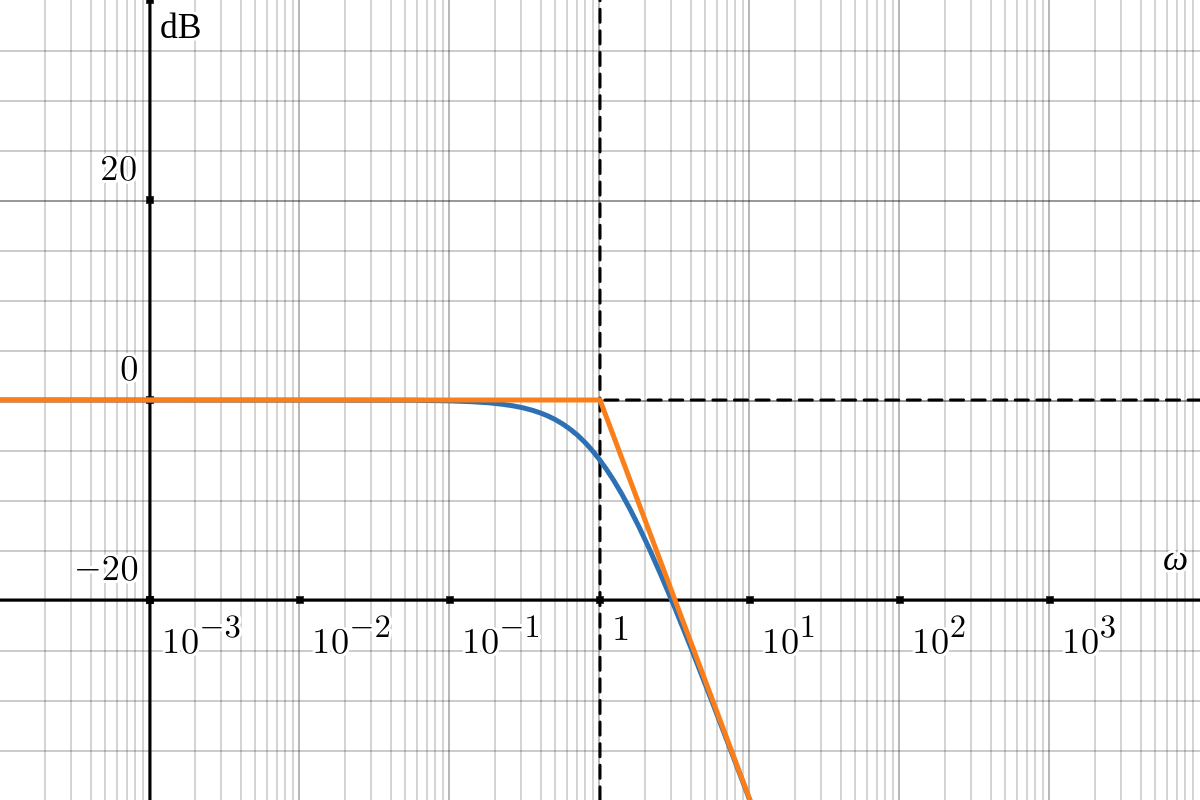
\includegraphics[scale=0.3]{../figures/order2_bode/clean_mod.png}
\end{center}
\end{minipage}

\par\bigskip

\subsubsection{Risonanza}
Potrebbe interessarci valutare l'errore, sopratutto considerato il fatto che non teniamo conto dello smorzamento $\xi$ nella stima per rette.
Prendiamo quindi il valore sul punto di rottura:
$$
|G(j\omega_0)|_{dB} = 20 \log \left( \frac{1}{4 \xi^2} \right) = -20 \log\left( 2 \xi \right) 
$$
per cui si ottengono gli errori al variare di $\xi$ (considerata la nostra approssimazione per rette che prende 0 dB a $\omega = \omega_0$):
\begin{table}[h!]
	\center \rowcolors{2}{white}{black!10}
	\begin{tabular} { c | c }
		$\mathbf{\xi}$ & \bfseries Errore \\ 
		\hline
		$0$ & $+\infty$ \\
		$\frac{1}{2}$ & 0 dB \\
		$\frac{\sqrt{2}}{2}$ & -3 dB \\
		$2$ & -6 dB \\
	\end{tabular}
\end{table}

Come regola empirica, possiamo assumere di poter usare il diagramma asintotico (il diagramma per rette) solo quando lo smorzamento è $\xi > 0.3$.

\par\bigskip

\noindent
\begin{minipage}{\textwidth}
Vediamo ad esempio l'errore che commettiamo per $\xi = \frac{1}{4}$, che calcoliamo subito dovrà essere di 6 dB:

\begin{center}
	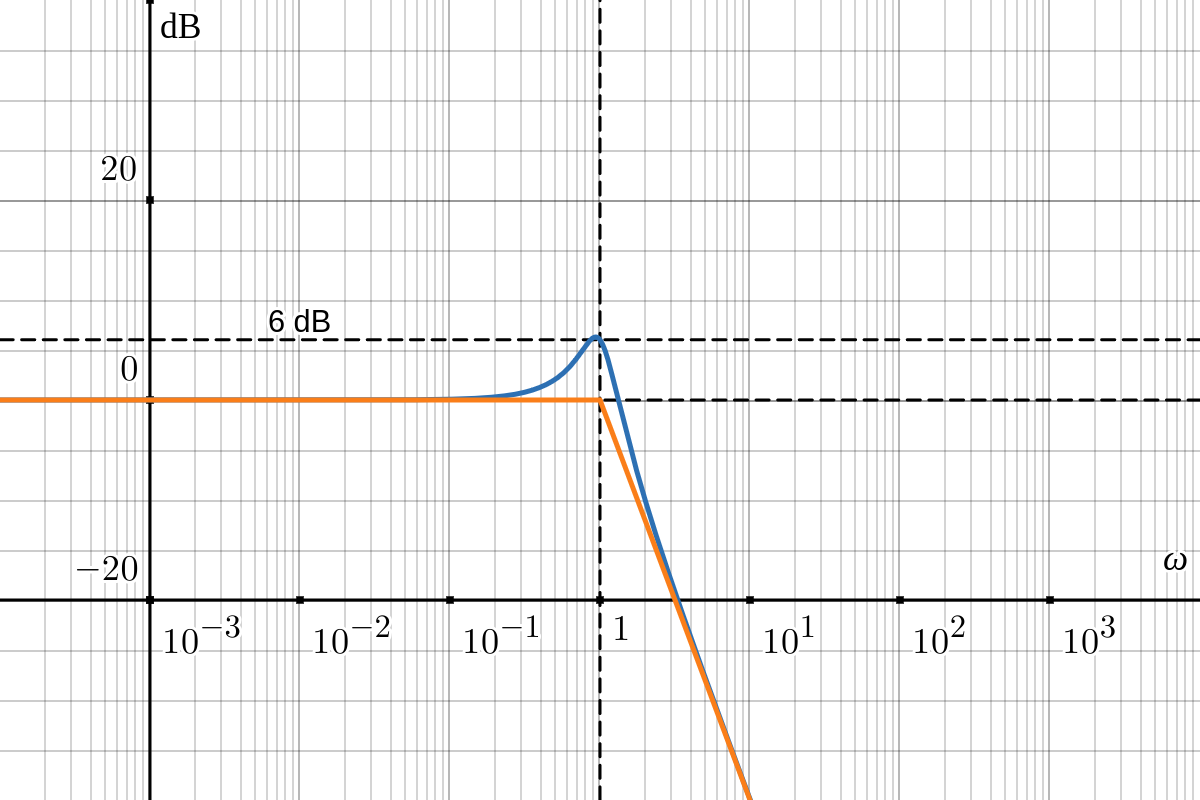
\includegraphics[scale=0.3]{../figures/order2_bode/reso_025_mod.png}
\end{center}
\end{minipage}

\par\bigskip

Come notiamo, si forma un picco attorno a $\omega = \omega_0$, dove la risposta ha un valore di picco vicino (in verità a $\xi$ decrescente il massimo assoluto si sposta sempre più verso sinistra) all'errore calcolato.
Questo picco prende il nome di \textbf{picco di risonanza}.

\subsubsection{Picco di risonanza}
Per ricavare il \textbf{punto di picco} effettivo, cerchiamo il punto stazionario della funzione:
$$
f(u) = (1 - u^2) + 4 \xi^2 u^2, \quad u= \frac{\omega}{\omega_0}
$$
che è il denominatore del modulo.

Abbiamo quindi, derivando:
$$
\frac{d}{du} f(u) = 0 = -4u(1 - u^2) + 8 \xi^2 u
$$
da cui:
$$
u_{max} = \frac{\omega_{max}}{\omega_0} = \sqrt{1 - 2 \xi^2}
$$
cioè il \textit{punto di picco} è:
$$
\omega_{max} = \omega_0 \sqrt{1 - 2 \xi^2} 
$$
e il \textit{valore di picco}, ovvero il modulo in decibel raggiunto nel punto di picco, è pari a:
$$
\max |G(j \omega)|_{dB} = 20 \log \left( |G(\omega_{max})| \right)
$$
Osserviamo che questo valore è effettivamente definito su $\mathbb{R}$ solo quando $\xi < \frac{1}{\sqrt{2}}$: questo si spiega semplicemente dal fatto che per $\xi > \frac{1}{\sqrt{2}}$ la funzione modulo del trasferimento è monotona, e non esiste nessun picco.

\par\bigskip

\noindent
\begin{minipage}{\textwidth}
Vediamo quindi il punto di picco dell'esempio precedente, dove ricordiamo avevamo preso $\xi = \frac{1}{4}$:

\begin{center}
	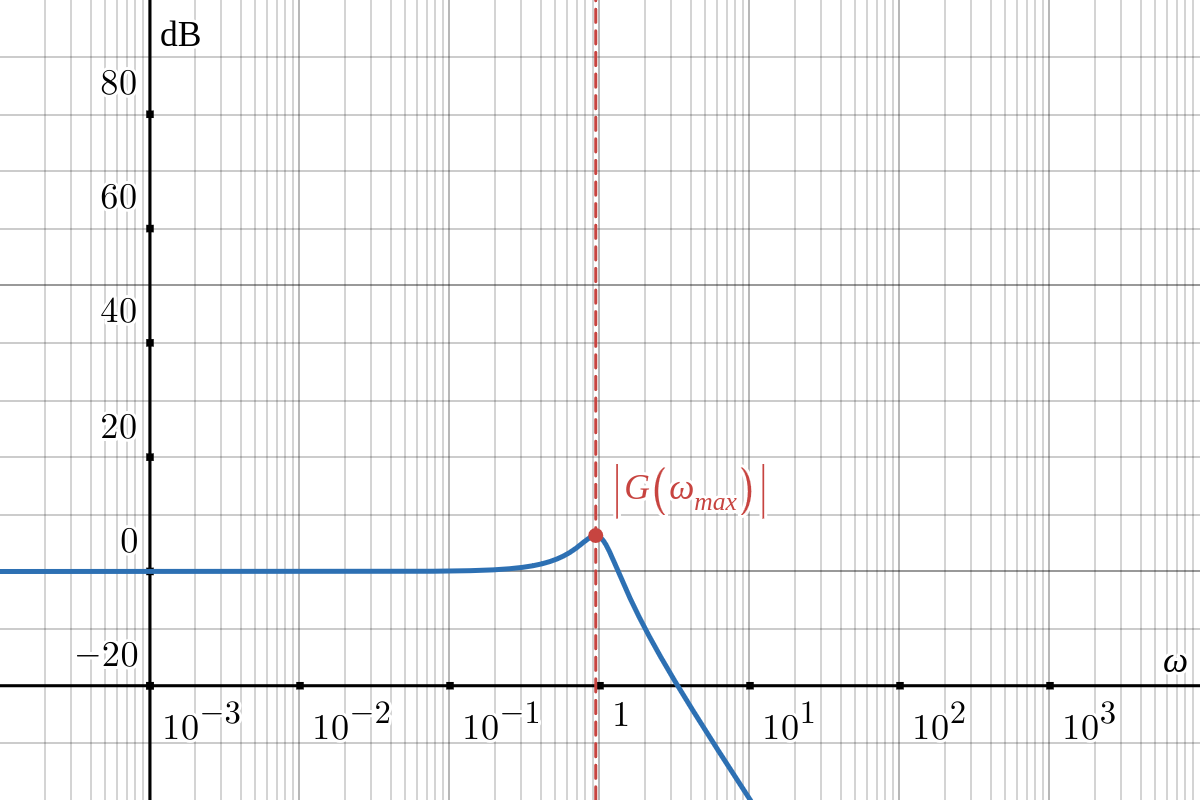
\includegraphics[scale=0.3]{../figures/order2_bode/peak_point.png}
\end{center}
\end{minipage}

\par\bigskip

Il valore $\omega_{max}$, calcolato al computer, risulta circa $\sim 0.935$, per cui l'errore $\left| G \left( \omega_{max} \right) \right|$ in questo caso è abbastanza vicino all'errore in $\omega = 1$, che era di 6 dB.

\par\bigskip

\noindent
\begin{minipage}{\textwidth}
Possiamo quindi riportare un grafico che mostra la variazione del picco di risonanza al variare dello smorzamento $\xi$:

\begin{center}
	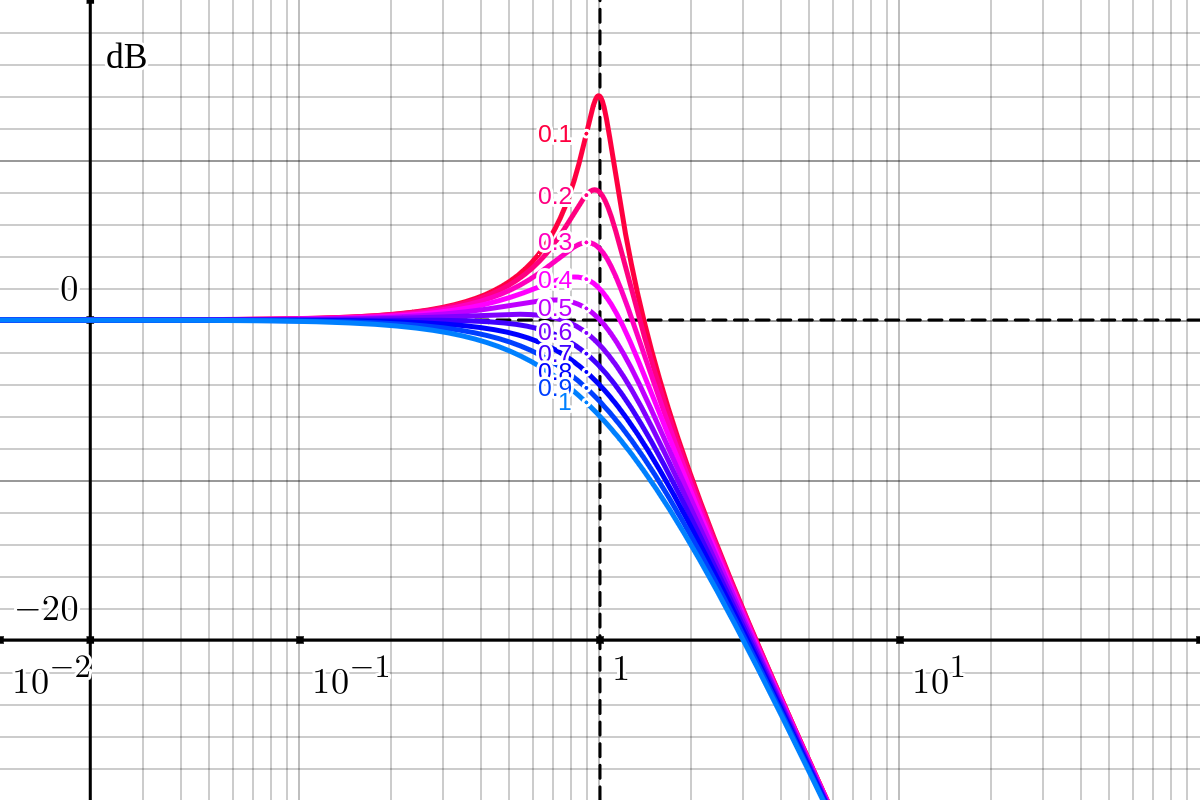
\includegraphics[scale=0.3]{../figures/order2_bode/peak_plot.png}
\end{center}
\end{minipage}

\par\bigskip

Questo grafico è duale a quello in 14.1.1: prima avevamo parlato della risposta a transiente, e adesso parliamo della risposta a regime, ma in entrambi i casi vediamo favorire una certa frequenza di oscillazione $\omega_0$ (che nel transiente avevamo visto è corretta di un fattore dipendente dallo smorzamento).

Inoltre, si vede molto bene come intorno a $0.7 \approx \frac{1}{\sqrt{2}}$ il picco scompare: questa è la conseguenza diretta del fatto che, come abbiamo detto, il punto di picco $\omega_0 \sqrt{1 - 2 \xi^2}$ è effettivamente definito su $\mathbb{R}$ solo nel caso $\xi < \frac{1}{\sqrt{2}}$.

\par\smallskip

Facciamo quindi un breve riassunto sulle frequenze di oscillazione che abbiamo incontrato finora:
\begin{itemize}
	\item \textbf{Frequenza di oscilazione naturale:} $\ \omega_0$ \\
		Abbiamo detto sarebbe la frequenza naturale a cui il sistema oscillasse se non vi fosse smorzamento $\xi$, e infatti vediamo che in tal caso corrisponde esattamente alle altre 2 frequenze; 
	\item \textbf{Frequenza di oscillazione naturale smorzata:} $\ \omega_d = \omega_0 \sqrt{1 - \xi^2}$ \\
		Rappresenta la frequenza di oscillazione della \textit{risposta libera} del sistema, cioè quella con cui, nel caso questo sia stabile, decade naturalmente al punto di equilibrio (l'origine); 
	\item \textbf{Frequenza di picco risonante:} $\ \omega_{max} = \omega_0 \sqrt{1 - 2 \xi^2}$ \\
		Rappresenta ciò che abbiamo appena visto, cioè la frequenza che il sistema, preso dal punto di vista della funzione di trasferimento ingresso-uscita, amplifica più delle altre (sotto l'ipotesi $\xi < \frac{1}{\sqrt2}$). In questo è intrinsecamente legata alla \textit{risposta forzata} del sistema.
\end{itemize}

Si ricava immediatamente che nei sistemi sottosmorzati $\xi < 1$ (che sono comunqe gli unici dove questo tipo di considerazioni si applicano), vale fra queste frequenze la relazione:
$$
\omega_{max} < \omega_d < \omega_0
$$
cioè il sistema preferisce oscillare, in \textit{risposta libera} ($\omega_d$), ad una frequenza leggermente più alta di quella di eccitazione massima in \textit{risposta forzata} ($\omega_{max}$).

\subsubsection{Valutazione di fase}
Per quanto riguarda la fase, invece, si avrà: 
$$
\angle G(j \omega) = -\mathrm{atan2} \left( \frac{ \frac{2\xi}{\omega_0}\omega }{ 1 - \frac{\omega^2}{\omega_0^2} } \right) 
$$
in quanto l'unico termine che determina la fase è il denominatore.

Potremo quindi prendere l'approssimazione per rette:
\[
	\begin{cases}
		\omega << \omega_0 \implies \angle G(j\omega) \approx 0^\circ \\ 	
		\omega >> \omega_0 \implies \angle G(j\omega) \approx -180^\circ \\ 	
		\omega = \omega_0 \implies \angle G(j\omega) = -90^\circ \\ 	
	\end{cases}
\]
preso $\tau > 0$.

Il valore in $\omega = \omega_0$ si calcola osservando che:
$$
\angle G(j \omega_0) = -\mathrm{atan2} \left( \frac{ 2 \xi }{ 0^+ } \right)
$$
da cui il limite, che porta appunto a $-90^\circ$.

\par\bigskip

\noindent
\begin{minipage}{\textwidth}
Otteniamo quindi il grafico approssimato, come sempre sovraimposto a quello reale:

\begin{center}
	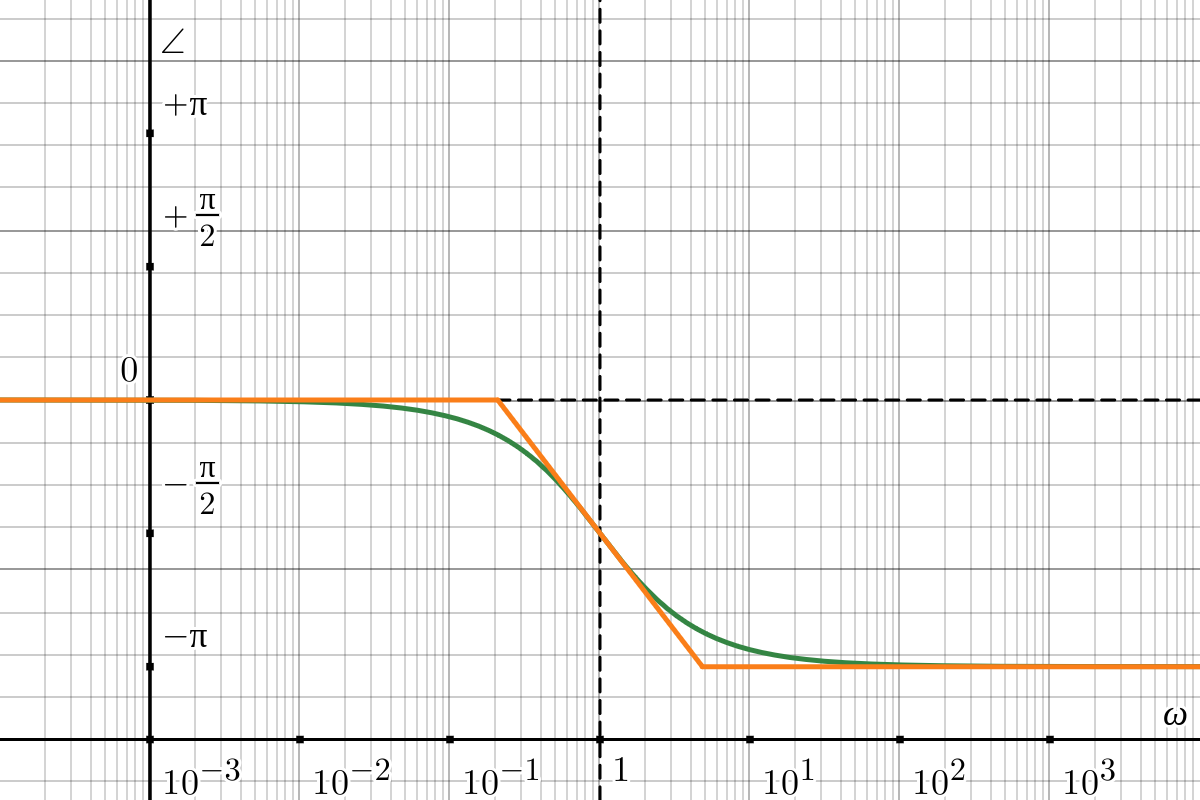
\includegraphics[scale=0.3]{../figures/order2_bode/phase.png}
\end{center}
\end{minipage}

\par\bigskip

Vediamo che lo scostamento in fase è lo stesso del sistema del primo ordine, ma raddoppiato: questo ha senso, in quanto abbiamo detto già lo stesso abbattimento dopo la frequenza di taglio $\omega_0$ era del doppio, cioè -40 dB/dec.

\par\smallskip

Una considerazione più interessante potrebbe essere quella della pendenza della retta che approssima la componente intorno a $\omega_0$: abbiamo infatti che, a differenza dei sistemi del prim'ordine, nei sistemi del second'ordine lo scostamento in fase avviene con velocità diverse intorno alla frequenza di taglio (finora si è assunto $-1$): è proprio questo a dare il caratteristico picco di risonanza (rispettate le condizioni di cui sopra).

Calcoliamo allora la derivata dell'argomento della risposta:
$$
\frac{d}{d\omega} \left( \angle G(j\omega) \right) 
= - \frac{1}{1 + \left( \frac{ \frac{2 \xi \omega}{\omega_0} }{ 1 - \frac{\omega^2}{\omega_0^2} } \right)^2 } 
\cdot \frac{ \frac{2 \xi}{\omega_0} \left( 1 - \frac{\omega^2}{\omega_0^2} \right) + \frac{2 \xi \omega}{\omega_0} \cdot \frac{2 \omega}{\omega_0^2} }{ \left( 1 - \frac{\omega^2}{\omega_0^2} \right)^2 }
$$
Questa funzione, valutata in $\omega_0$, dà:
$$
\frac{d}{d\omega} \left( \angle G(j\omega) \right) (j \omega_0) = - \frac{2 \xi}{\omega_0} \cdot \frac{ \left( 1 + \frac{\omega_0^2}{\omega_0^2} \right) }{ \left( 1 - \frac{\omega_0^2}{\omega_0^2} \right)^2 + \left( \frac{2 \xi \omega_0}{\omega_0} \right)^2 } = - \frac{1}{\xi \omega_0}
$$
Tracceremo quindi la retta di congiunzione in $\omega = \omega_0$ con coefficiente angolare $- \frac{1}{\xi \omega_0}$.

\par\bigskip

\noindent
\begin{minipage}{\textwidth}
Vediamo ad esempio il caso con $\xi = 0.6$:

\begin{center}
	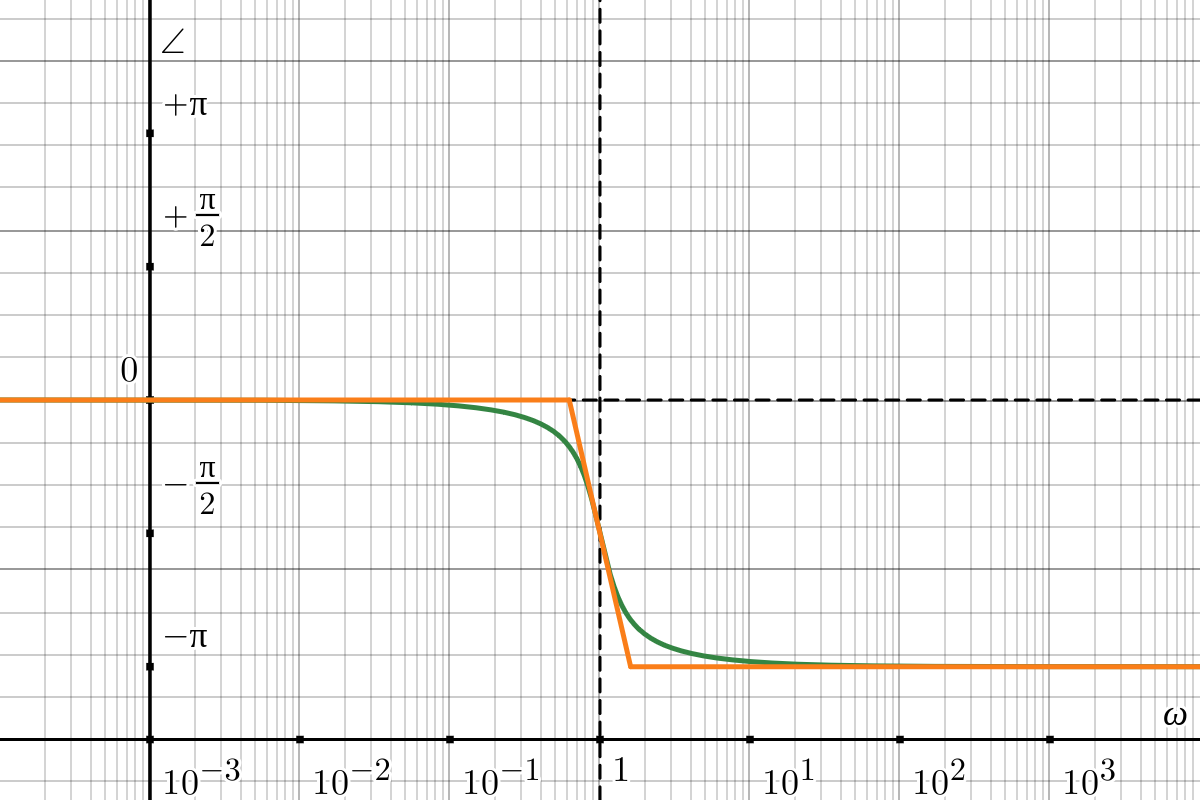
\includegraphics[scale=0.3]{../figures/order2_bode/phase_weird.png}
\end{center}
\end{minipage}

\par\bigskip

Dal punto di vista pratico, possiamo fare la stessa ipotesi di approssimazione di prima: per $\xi > 0.3$ prendiamo la retta con derivata $-1$, mentre per $\xi < 0.3$ la pendenza è troppo ripida perchè questa sia valida.

\subsection{Ritardo nei diagrammi di Bode}
Vediamo infine l'effetto che il ritardo ha nel dominio frequenze.
Avevamo già visto l'espressione del ritardo nel dominio d Laplace:
$$
G(s) = e^{-s \tau}
$$
In risposta armonica, questa dà:
$$
G(j \omega) = e^{-j \omega \tau}
$$
cioè uno scostamento in fase di $\omega \tau$.

L'effetto sul diagramma di Bode sarà quindi di lasciare invariato il modulo (cioè dare una costante a 0 dB), e sopratutto di scostare la fase di un valore pari a $-\omega \tau$.

\par\bigskip

\noindent
\begin{minipage}{\textwidth}
Vediamo allora il grafico del modulo:

\begin{center}
	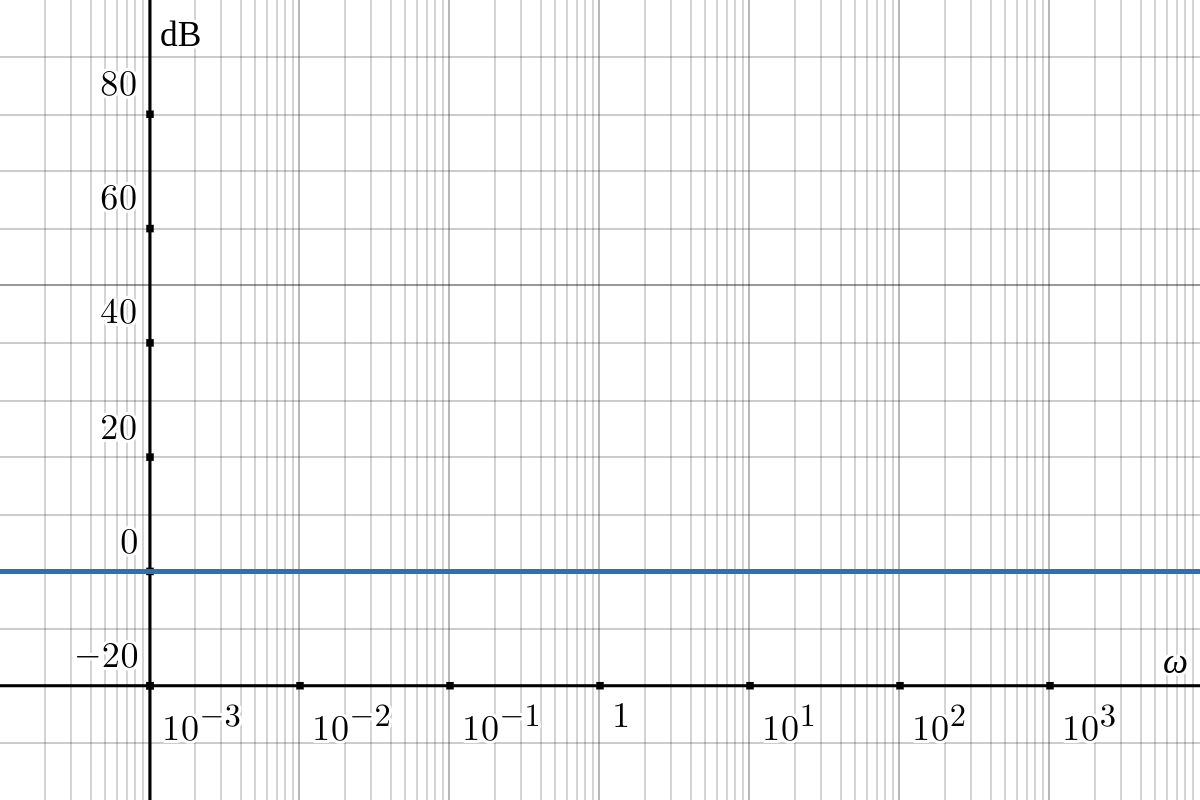
\includegraphics[scale=0.3]{../figures/delay_bode/mod.png}
\end{center}
\end{minipage}

\par\bigskip

\noindent
\begin{minipage}{\textwidth}
e il grafico della fase:

\begin{center}
	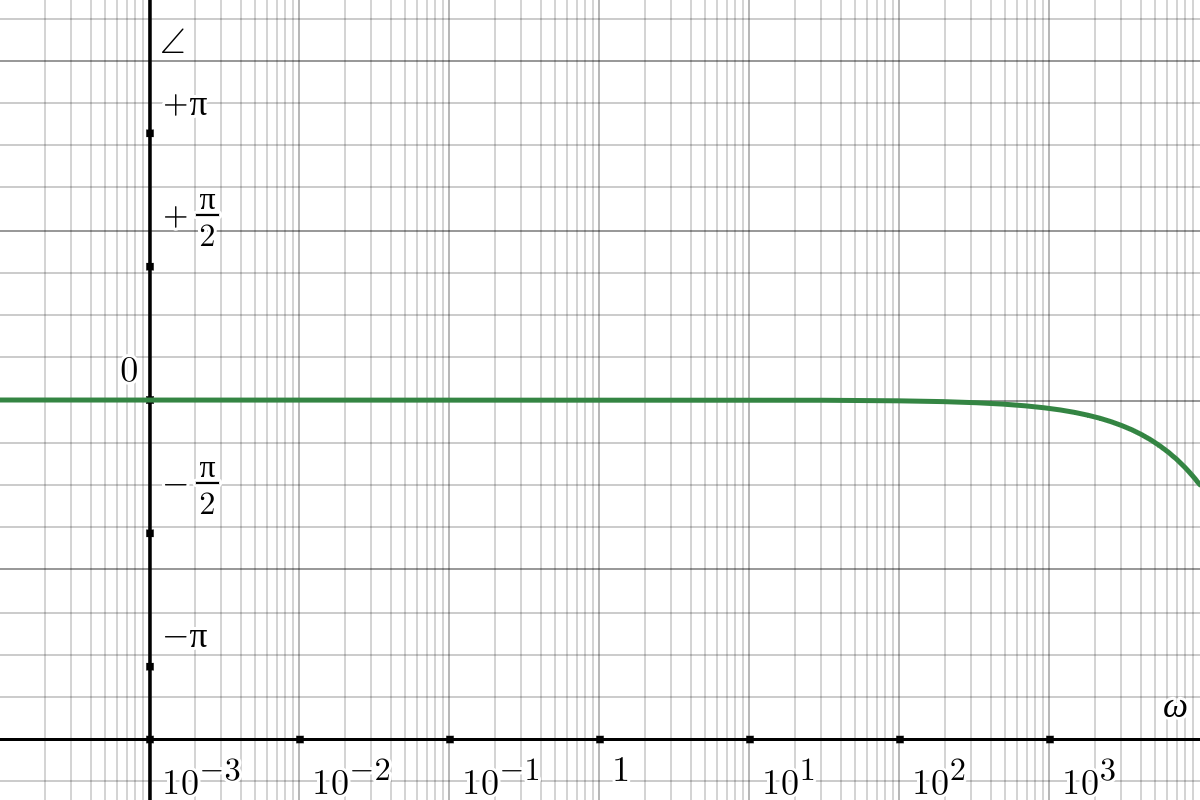
\includegraphics[scale=0.3]{../figures/delay_bode/phase.png}
\end{center}
\end{minipage}

\par\bigskip

\subsection{Esempio: diagramma di Bode}
Vediamo quindi un esempio pratico di disegno di un diagramma di Bode.
Prendiamo la funzione di trasferimento:
$$
G(s) = 200 \frac{\left( s+ \frac{1}{10} \right)}{ (s + 1) \left( \frac{s^2}{400} + \frac{s}{20} + 1 \right) }
$$
che protiamo subito nella forma di Bode e in risposta armonica:
$$
= 20 \frac{\left( 10s + 1 \right)}{ (s + 1) \left( \frac{s^2}{400} + \frac{s}{20} + 1 \right) } 
= 20 \frac{\left( 10 j \omega + 1 \right)}{ (j \omega + 1) \left( -\frac{\omega^2}{400} + \frac{j \omega}{20} + 1 \right) }
$$

Vediamo poi il guadagno: questo nella forma di Bode è dato dal $20$ che moltiplica il rapporto polinomi.
Dalla tabella in 17.2.1 ricordiamo che un modulo di $|20|$ corrisponde a un guadagno di 26 dB.
Aggiugneremo quindi questo valore a tutti i moduli che calcoleremo.

Da qui distinguiamo zeri e poli e ne individuiamo il comportamento tramite un approssimazione per rette.
Da quanto avevamo dimostrato nella 17.1.3, potremo poi sommare i grafici ottenuti dalle singole risposte per zero e per polo e ottenere la risposta complessiva.

Abbiamo quindi:
\begin{itemize}
	\item \textbf{Zeri:}
		\begin{itemize}
			\item $10 j \omega + 1$: questo rappresenta una rampa, con pendenza di 20 dB/dec, che inizia a pulsazione $j \omega^* = \frac{1}{10}$. \\ 
				Dal punto di vista della fase rappresenterà una transizione da $0^\circ$ a $90^\circ$ con punto a derivata unitaria in $\frac{1}{10}$.
		\end{itemize}
	\item \textbf{Poli:}
		\begin{itemize}
			\item $j \omega + 1$: questo rappresenta un passa basso, con pendenza di -20 dB/dec e frequenza di taglio a $j \omega^* = 1$. \\ 
				Dal punto di vista della fase rappresenterà una transizione da $0^\circ$ a $-90^\circ$ con punto a derivata unitaria in $1$;
			\item $-\frac{\omega^2}{400} + \frac{j \omega}{20} + 1$: questa è una forma del secondo grado, di cui ci interessa prima di tutto conoscere il tipo.
				Riconosciamo allora di poterci ricondurre alla forma $-\frac{\omega^2}{\omega_0^2} + \frac{2\xi}{\omega_0} j \omega + 1$, cioè:
				$$
				-\frac{\omega^2}{400} + \frac{j \omega}{20} + 1 = -\frac{\omega^2}{\omega_0^2} + \frac{2\xi}{\omega_0} j \omega + 1
				$$
				da cui:
				$$
				\omega_0^2 = 400 \implies \omega_0 = 20, \quad \frac{2\xi}{\omega_0} = \frac{2\xi}{20} = \frac{1}{20} \implies \xi = \frac{1}{2}
				$$
				cioè siamo nel caso sottosmorazato, tra con l'altro $\xi = 0.5$, che è compreso fra $0.3$ e $0.7$, quindi abbiamo detto \textit{risonante} ma \textit{approssimabile} col diagramma a rette.
				Ignoriamo quindi lo smorzamento e prendiamo un filtro passa basso con pendenza di -40 dB/dec e frequenza di taglio a $j \omega^* = 20$. \\ 
				Dal punto di vista della fase rappresenterà una transizione da $0^\circ$ e $-90^\circ$
		\end{itemize}
\end{itemize}

Tracciamo quindi il diagramma di Bode del modulo, considerando le seguenti regioni:
\begin{itemize}
	\item $[0, 0.1)$: nessun zero o polo è attivo, quindi si resta a 0 + 26 dB;
	\item $[0.1, 1)$: lo zero è attivo, si sale con 20 dB/dec fino a 20 + 26dB;
	\item $[1, 20)$: il polo lineare è attivo e compensa lo zero, si resta a 20 + 26 dB;
	\item $[20, +\infty)$: il polo quadratico è attivo, si scende con -40 db/dec.
\end{itemize}

\par\bigskip

\noindent
\begin{minipage}{\textwidth}
da cui il grafico:

\begin{center}
	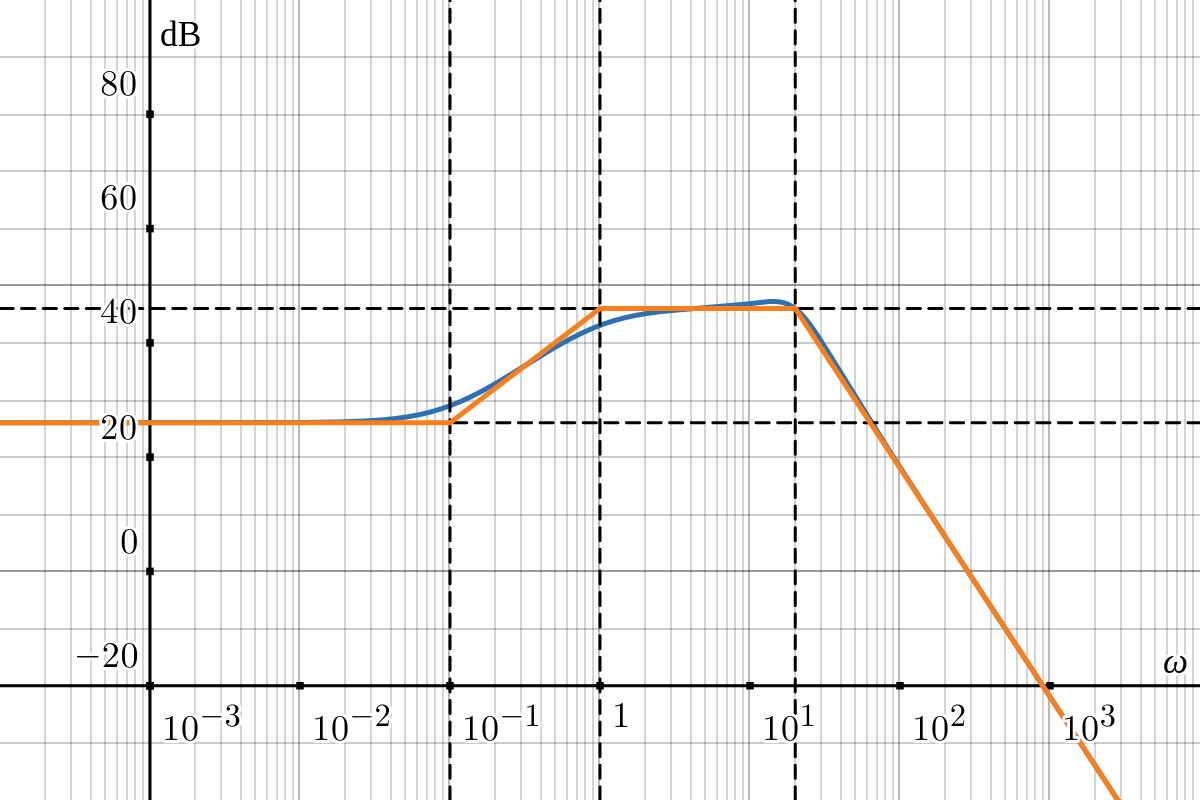
\includegraphics[scale=0.3]{../figures/exerc_bode.png}
\end{center}
\end{minipage}

\par\bigskip

che come vediamo si discosta dal grafico originale per lo più per lo smussamento intorno a $0.1 \sim 1$, e per il picco di risonanza (che abbiamo volontariamente ignorato) a $20$.

\par\smallskip

Disegnamo quindi il diagramma di Bode della fase.
In questo caso notiamo di avere molta sovrapposizione fra le transizioni di fase: un'idea potrebbe essere quella di considerare assoluti solo i valori agli estremi $0$ e a $+\infty$, e per gli zeri e i poli intermedi prendere i punti "medi" (a $\pm 45^\circ$ per lo zero e il polo lineare, e a $-90^\circ$ per il polo quadratico).

\par\bigskip

\noindent
\begin{minipage}{\textwidth}

\begin{center}
	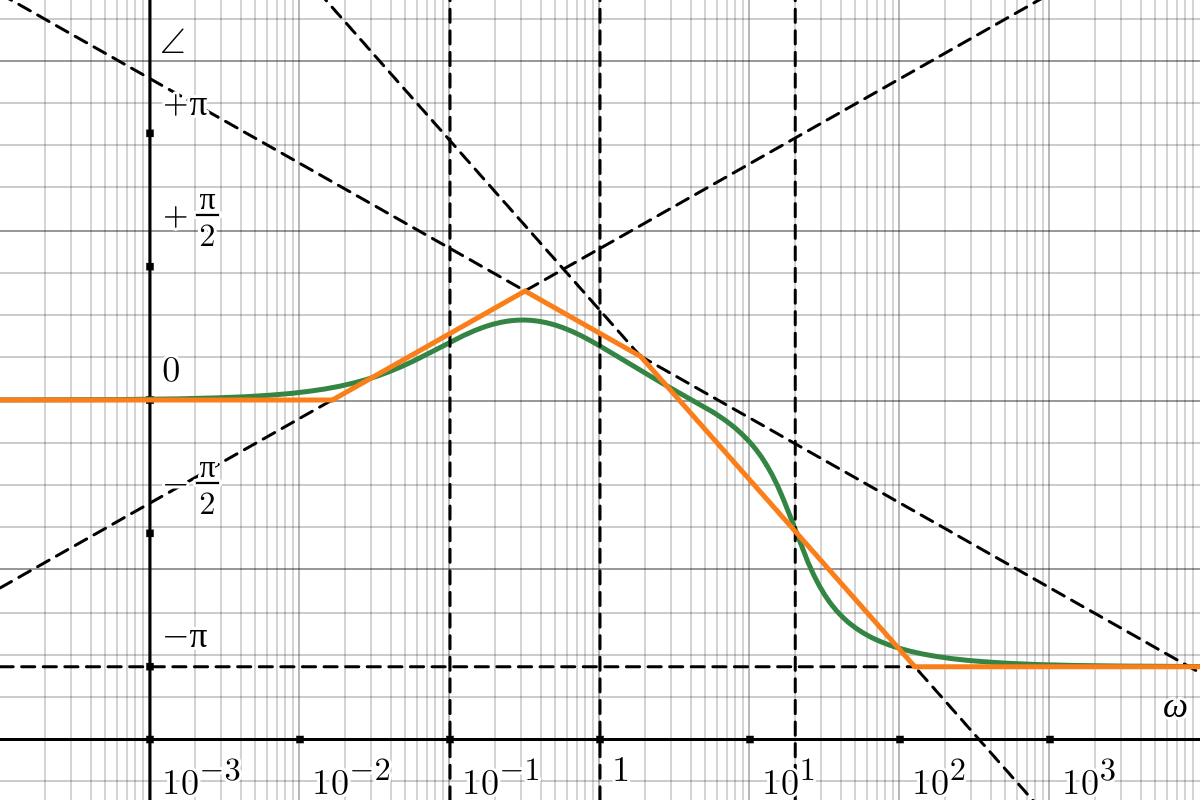
\includegraphics[scale=0.3]{../figures/exerc_bode_phase.png}
\end{center}
\end{minipage}

\par\bigskip

che vediamo essere abbastanza simile alla fase effettiva (in verde).

\end{document}


\documentclass[a4paper,11pt]{article}
\usepackage[a4paper, margin=8em]{geometry}

% usa i pacchetti per la scrittura in italiano
\usepackage[french,italian]{babel}
\usepackage[T1]{fontenc}
\usepackage[utf8]{inputenc}
\frenchspacing 

% usa i pacchetti per la formattazione matematica
\usepackage{amsmath, amssymb, amsthm, amsfonts}

% usa altri pacchetti
\usepackage{gensymb}
\usepackage{hyperref}
\usepackage{standalone}

% imposta il titolo
\title{Appunti Fondamenti di Automatica}
\author{Luca Seggiani}
\date{2025}

% disegni
\usepackage{pgfplots}
\pgfplotsset{width=10cm,compat=1.9}

% imposta lo stile
% usa helvetica
\usepackage[scaled]{helvet}
% usa palatino
\usepackage{palatino}
% usa un font monospazio guardabile
\usepackage{lmodern}

% tikz in sans
\tikzset{every picture/.style={/utils/exec={\sffamily}}}

\renewcommand{\rmdefault}{ppl}
\renewcommand{\sfdefault}{phv}
\renewcommand{\ttdefault}{lmtt}

% circuiti
\usepackage{circuitikz}
\usetikzlibrary{babel}

% disponi il titolo
\makeatletter
\renewcommand{\maketitle} {
	\begin{center} 
		\begin{minipage}[t]{.8\textwidth}
			\textsf{\huge\bfseries \@title} 
		\end{minipage}%
		\begin{minipage}[t]{.2\textwidth}
			\raggedleft \vspace{-1.65em}
			\textsf{\small \@author} \vfill
			\textsf{\small \@date}
		\end{minipage}
		\par
	\end{center}

	\thispagestyle{empty}
	\pagestyle{fancy}
}
\makeatother

% disponi teoremi
\usepackage{tcolorbox}
\newtcolorbox[auto counter, number within=section]{theorem}[2][]{%
	colback=blue!10, 
	colframe=blue!40!black, 
	sharp corners=northwest,
	fonttitle=\sffamily\bfseries, 
	title=Teorema~\thetcbcounter: #2, 
	#1
}

% disponi definizioni
\newtcolorbox[auto counter, number within=section]{definition}[2][]{%
	colback=red!10,
	colframe=red!40!black,
	sharp corners=northwest,
	fonttitle=\sffamily\bfseries,
	title=Definizione~\thetcbcounter: #2,
	#1
}

% disponi problemi
\newtcolorbox[auto counter, number within=section]{problem}[2][]{%
	colback=green!10,
	colframe=green!40!black,
	sharp corners=northwest,
	fonttitle=\sffamily\bfseries,
	title=Problema~\thetcbcounter: #2,
	#1
}

% disponi codice
\usepackage{listings}
\usepackage[table]{xcolor}

\lstdefinestyle{codestyle}{
	backgroundcolor=\color{black!5}, 
	commentstyle=\color{codegreen},
	keywordstyle=\bfseries\color{magenta},
	numberstyle=\sffamily\tiny\color{black!60},
	stringstyle=\color{green!50!black},
	basicstyle=\ttfamily\footnotesize,
	breakatwhitespace=false,         
	breaklines=true,                 
	captionpos=b,                    
	keepspaces=true,                 
	numbers=left,                    
	numbersep=5pt,                  
	showspaces=false,                
	showstringspaces=false,
	showtabs=false,                  
	tabsize=2
}

\lstdefinestyle{shellstyle}{
	backgroundcolor=\color{black!5}, 
	basicstyle=\ttfamily\footnotesize\color{black}, 
	commentstyle=\color{black}, 
	keywordstyle=\color{black},
	numberstyle=\color{black!5},
	stringstyle=\color{black}, 
	showspaces=false,
	showstringspaces=false, 
	showtabs=false, 
	tabsize=2, 
	numbers=none, 
	breaklines=true
}

\lstdefinelanguage{javascript}{
	keywords={typeof, new, true, false, catch, function, return, null, catch, switch, var, if, in, while, do, else, case, break},
	keywordstyle=\color{blue}\bfseries,
	ndkeywords={class, export, boolean, throw, implements, import, this},
	ndkeywordstyle=\color{darkgray}\bfseries,
	identifierstyle=\color{black},
	sensitive=false,
	comment=[l]{//},
	morecomment=[s]{/*}{*/},
	commentstyle=\color{purple}\ttfamily,
	stringstyle=\color{red}\ttfamily,
	morestring=[b]',
	morestring=[b]"
}

% disponi sezioni
\usepackage{titlesec}

\titleformat{\section}
{\sffamily\Large\bfseries} 
{\thesection}{1em}{} 
\titleformat{\subsection}
{\sffamily\large\bfseries}   
{\thesubsection}{1em}{} 
\titleformat{\subsubsection}
{\sffamily\normalsize\bfseries} 
{\thesubsubsection}{1em}{}

% disponi alberi
\usepackage{forest}

\forestset{
	rectstyle/.style={
		for tree={rectangle,draw,font=\large\sffamily}
	},
	roundstyle/.style={
		for tree={circle,draw,font=\large}
	}
}

% disponi algoritmi
\usepackage{algorithm}
\usepackage{algorithmic}
\makeatletter
\renewcommand{\ALG@name}{Algoritmo}
\makeatother

% disponi numeri di pagina
\usepackage{fancyhdr}
\fancyhf{} 
\fancyfoot[L]{\sffamily{\thepage}}

\makeatletter
\fancyhead[L]{\raisebox{1ex}[0pt][0pt]{\sffamily{\@title \ \@date}}} 
\fancyhead[R]{\raisebox{1ex}[0pt][0pt]{\sffamily{\@author}}}
\makeatother

\begin{document}

% sezione (data)
\section{Lezione del 15-04-25}

% stili pagina
\thispagestyle{empty}
\pagestyle{fancy}

% testo
\subsubsection{Approssimazione del punto di crossover a 0 dB}
Potrebbe esserci di interesse trovare quando il diagramma del modulo di una risposta in frequenza interseca l'asse a 0 dB.

Preso ad esempio l'esempio della scorsa lezione, che avevamo portato in forma di Bode:
$$
G(s) = 20 \frac{\left( 10s + 1 \right)}{ (s + 1) \left( \frac{s^2}{400} + \frac{s}{20} + 1 \right) } 
$$
possiamo procedere in 2 modi:
\begin{itemize}
	\item Calcolando il valore approssimato ottenuto nell'ultimo zero o polo agente, e l'ultima salita/discesa in dB/oct o dB/dec che osserviamo nel grafico, e quindi cercando l'intersezione del grafico.

		Nell'esempio precedente avremo quindi l'ultimo punto fisso a 46 dB, con una discesa da questo in poi di -40 dB/dec.
		Avremo quindi che l'andamento della risposta in modulo da $\omega = 200$ in poi:
		$$
		|G(j \omega)|_{dB} = 46 - 40 \log\left( \frac{\omega}{20} \right)
		$$
		da cui imponendo a 0:
		$$
		0 = 46 - 40 \log\left( \frac{\omega}{20} \right) \implies \omega^* = 20 \cdot 10^{\frac{46}{40}} \approx 282.51
		$$
		cioè risulta che a $\sim 282.84$ rad/s si ha il punto di intersezione in 0 dB.

	\item Sommando (che in dB significa moltiplicando) le approssimazioni asintotiche di ogni termine al numeratore e denominatore, quindi ogni zero e polo, e imponendo il loro rapporto all'unità (come abbiamo detto, 0 dB significà unità).

		Nell'esempio precedente vorremmo partire dalla costante:
		$$
		G(s) \approx 20
		$$
		e quindi moltiplicare per l'approssimazione asintotica dello zero, che è il solo termine in $s$, $10s$:
		$$
		\approx 20 \cdot 10s = 200s
		$$
		Dividiamo quindi per il polo lineare, prendendo ancora solo il termine in $s$, cioè $s$ stesso:
		$$
		\approx \frac{200s}{s} = 200
		$$
		e infine dividiamo per il polo quadratico, per cui come approssimazione asintotica prendiamo il termine di grado massimo in, $\frac{s^2}{400}$:
		$$
		\approx 200 \cdot \frac{400}{s^2}
		$$
		Imponendo qindi l'unità si ottiene:
		$$
		\frac{80000}{s^2} = 1 \implies s = \sqrt{80000} \approx 282.84
		$$
		cioè risulta a $\sim 282.84$ rad/s si ha il punto di intersezione in 0 dB, che è abbastanza vicino alla stima precedente.
\end{itemize}

\subsection{Luogo delle radici}
Il luogo delle radici è un metodo per studiare sul piano complesso l'effetto della reazione negativa sui poli del sistema in catena chiusa, assunto di conoscere la funzione di trasferimento in catena aperta $G(s)$, cioè secondo quanto già visto in 15.2, da cui riportiamo il grafico:
\begin{center}
	\begin{tikzpicture}
		\draw (1,0) rectangle (3, 1);
		\node at (2, 0.5) {$G(s)$};

		\draw (-3,0) rectangle (-1, 1);
		\node at (-2, 0.5) {$C(s)$};

		\draw (-1.5, -0.5) rectangle (0.5, -1.5);
		\node at (-0.5, -1) {$H(s)$};

		\draw[-stealth] (-7, 0.5) -> (-5.1, 0.5);
		\draw[-stealth] (-5, 0.5) -> (-3, 0.5);
		\draw[-stealth] (-1, 0.5) -> (1, 0.5);
		\draw[-stealth] (3, 0.5) -> (3.9, 0.5);
		\draw[-stealth] (4, 0.5) -> (7, 0.5);

		\draw (5, 0.5) -> (5, -1);
		\draw[-stealth] (5, -1) -> (0.5, -1);
		\draw (-1.5, -1) -> (-5, -1);
		\draw[-stealth] (-5, -1) -> (-5, 0.5);

		\draw[-stealth] (4, 1.5) -> (4, 0.6);
		\node at (4, 1.75) {disturbo};

		\draw[fill=white] (-5, 0.5) circle (0.1);
		\draw[fill=white] (4, 0.5) circle (0.1);

		\node at (-6, 0.75) {$R(s)$};
		\node at (6, 0.75) {$Y(s)$};

		\node at (-4.75, 0.75) {$+$};
		\node at (-4.75, 0.25) {$-$};

		\node at (-3.8, 0.75) {\textit{errore}};
		\node at (0, 0.75) {\textit{controllo}};
		\node at (-3.5, -1.5) {\textit{feedback}};
	\end{tikzpicture}
\end{center}
assunto, come sempre, $H(s)$ sensore all'unità e disturbi trascurabili.

Facciamo quindi l'ulteriore semplificazione di prendere il controllore come una \textit{costante proporzionale}, cioè:
$$
C(s) = K
$$

Il luogo delle radici permette quindi l'analisi \textit{grafico-visuale} delle variazioni dei poli in catena chiusa al variare di uno o più parametri (eventualmente introdotti da un controllore).

\subsubsection{Equazione caratteristica}
Avremo quindi che, sotto le ipotesi di cui sopra, le risposte saranno:
\begin{itemize}
	\item In \textbf{circuito aperto}:
		$$
		K \cdot G(s) = K \cdot \frac{\prod_{i = 1}^m (s - z_i)}{\prod_{i = 1}^n (s - p_i)} = K \cdot \frac{n(s)}{d(s)}
		$$
	\item In \textbf{circuito aperto}:
		$$
		W(s) = \frac{K \cdot G(s)}{1 + K \cdot G(s)} = \frac{K \cdot n(s)}{d(s) + K \cdot n(s)}
		$$
\end{itemize}

I poli in catena chiusa saranno quindi le radici del polinomio:
$$
d(s) + K \cdot n(s)
$$
chiamiamo infatti la seguente equazione:
$$
d(s) + K \cdot n(s) = 0
$$
\textbf{equazione caratteristica} del sistema in catena chiusa.

Il \textbf{luogo delle radici} in sé per sé sarà quindi l'insieme delle radici dell'equazione caratteristica al variare di $K$.

\subsubsection{Regole di tracciamento 1}
Vediamo allora una serie di \textit{regole} che possiamo usare per tracciare il luogo delle radici:

\begin{enumerate}
	\item 
		Varrà quindi la regola (1), cioè che il numero di radici in ciclo chiuso è uguale al numero di poli della funzione $G$ in ciclo aperto.
		Questo significa che il numero di \textit{rami} del luogo delle radici è uguale al numero di poli della funzione di trasferimento in ciclo aperto.

		In particolare, diciamo che il numeratore $n(s)$ ha grado $m$ e il denominatore $d(s)$ ha grado $n$, con $n \geq m$.
		Questo coincide con la definizione che abbiamo dato prima della $G(s)$, che era:
		$$
		G(s) = \frac{\prod_{i = 1}^m (s - z_i)}{\prod_{i = 1}^n (s - p_i)}
		$$
		Avremo allora che l'equazione caratteristica ha grado $n$, cioè si hanno tante radici dell'equazione caratteristica quanti sono i poli della funzione di trasferimento in ciclo aperto.

		\par\medskip
		\noindent
		\textbf{\sffamily{Esempio}}

		Introduciamo la funzione di trasferimento di esempio:
		$$
		G(s) = \frac{1}{s (s + 1)}
		$$
		Cioè:
		$$
		n(s) = 1, \quad d(s) = s(s + 1)
		$$
		in questo caso varrà che $m = 0$ (non ci sono zeri) e $n = 2$, cioè ci aspetteremo di trovare due rami.

	\item	
		La regola (2) riguarda la caratterizzazione geometrica del luogo delle radici. Riprendendo l'equazione caratteristica, potremo infatti dire:
		$$
		d(s) + K \cdot n(s) = 0 \implies \frac{n(s)}{d(s)} = -\frac{1}{K}
		$$
		Da questa ricaviamo due condizioni di appartenenza al luogo delle radici, rispettivamente in \textit{fase} e in \textit{modulo}.
		\begin{itemize}
			\item 
				Si definisce la cosiddetta \textbf{condizione di fase}:
				\[
					\begin{cases}
						\angle n(s) - \angle d(s) = -\pi \pm 2 h \pi, \quad K > 0 \\
						\angle n(s) - \angle d(s) = \pm 2 h \pi, \quad K < 0
					\end{cases}
				\]
				Questa deriva dal fatto che. per le proprietà stesse del prodotto complesso, vale:
				$$
				\angle \left( \frac{n(s)}{d(s)} \right) = \angle n(s) - \angle d(s)
				$$
				mentre il termine a destra, essendo $K$ un reale, sarà $-\pi$ se $K > 0$, e $0$ viceversa.
				I termini $2 h \pi$, con $h \in \mathbb{N}$, vengono introdotti perché ruotando di $360^\circ$ gradi sul piano complesso si torna da dove si è partiti.
				Vediamo quindi che applicare la condizione di fase significa costruire il luogo delle radici, cioè questa condizione da sola basta a ricavare tutto il luogo.

				Possiamo dare un'ulteriore interpretazione geometrica degli angoli.
				Si ha infatti che vale, sempre per le proprietà dei complessi, rispetto a un qualsiasi punto $s$:
				\[
					\begin{cases}
						\angle n(s) = \arg \prod_{i = 1}^m (s + z_i) = \sum_{i = 1}^m (s + z_i) = \sum_{i = 1}^m \theta_i \\ 
						\angle d(s) = \arg \prod_{j = 1}^n (s + p_j) = \sum_{j = 1}^n (s + p_j) = \sum_{j = 1}^n \phi_j 
					\end{cases}
				\]
				dove $\phi_j$ e $\theta_i$ rappresentano gli angoli le congiungenti con i poli in $j$ e gli zeri in $i$ formano con l'asse reale. 

				\par\medskip
				\noindent
				\textbf{\sffamily{Esempio}}

				Riprendiamo il polinomio:
				$$
				G(s) = \frac{1}{s (s + 1)}
				$$
				possiamo anticipare che i suoi poli sono $p_1 = 0$ e $p_2 = -1$.
				In questo caso, preso ad esempio il punto $s = -\frac{1}{2} + i$ si avranno gli angoli:

				\begin{center}
					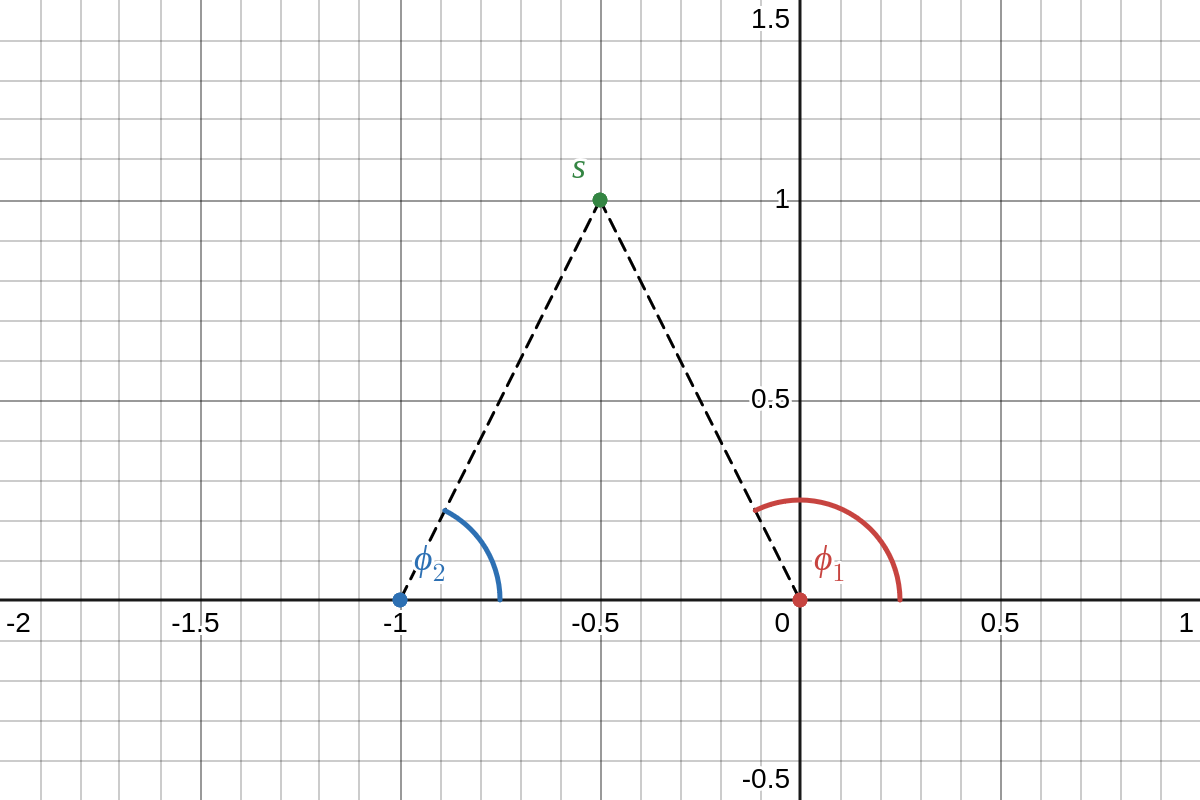
\includegraphics[scale=0.26]{../figures/locus_phi.png}
				\end{center}

			\item
				Nessuno ci nega di costruire anche una \textbf{condizione di modulo}, cioè imporre ai soli moduli:
				$$
				\left| \frac{n(s)}{d(s)} \right| = \frac{1}{|K|}
				$$
				Vediamo che questa condizione non è indispensabile, ma invece applicarla significa "tarare" il luogo delle radici su un singolo valore di $K$.

				Abbiamo anche qui un'interpretazione geometrica analoga a quella degli angoli.
				Potremo infatti dire:
				$$
				|n(s)| = \prod_{i = 1}^m |s + z_i|, \quad |d(s)| = \prod_{i = 1}^n |s + p_i|
				$$
				dove gli $|s^* + z_i| = \lambda_i$ e $|s^* + p_i| = \eta_i$ corrispondono alle distanze del generico punto nel luogo $s^*$, per cui:
				$$
				|K| = \frac{ \prod_{i = 1}^n |s^* + p_i| }{ \prod_{i = 1}^m |s^* + z_i| } = \frac{ \prod_{i = 1}^n \eta_i }{ \prod_{i = 1}^m \lambda_i }
				$$
				Cioè il guadagno $K$ per un certo punto $s^*$ corrisponde al rapporto fra il prodotto delle distanze dai poli e il prodotto delle distanze dagli zeri.

				\par\medskip
				\noindent
				\textbf{\sffamily{Esempio}}

				Riprendiamo il polinomio:
				$$
				G(s) = \frac{1}{s (s + 1)}
				$$
				conosciamo i suoi $p_1 = 0$ e $p_2 = -1$.
				In questo caso, preso lo steso punto $s = -\frac{1}{2} + i$ di prima (che anticipiamo far parte del luogo) si avranno le distanze:

				\begin{center}
					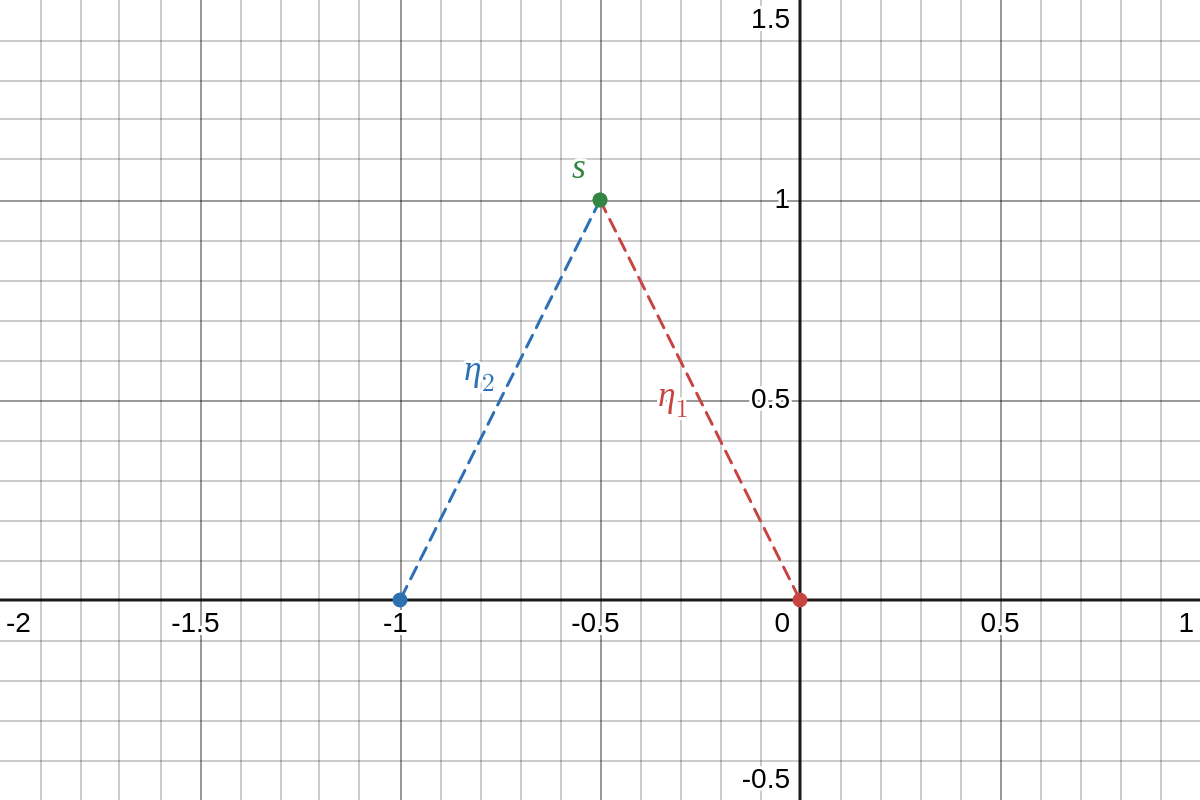
\includegraphics[scale=0.26]{../figures/locus_eta.png}
				\end{center}

		\end{itemize}

	\item
		Potremo quindi ricavare la regola (3), che riguarda l'andamento in funzione di $K$ del luogo, cioè dire che preso:
		$$
		d(s) + K \cdot n(s) = 0
		$$
		ponendo $K = 0$ si nota che il luogo parte dai \textbf{poli a ciclo aperto} del sistema (cioè da $d(s) = 0$);

		Di contro, preso:
		$$
		\frac{1}{K} \cdot d(s) + n(s) = 0
		$$
		ponendo $K = +\infty$ si nota che il luogo arriva agli \textbf{zeri a ciclo aperto} del sistema (cioè $n(s) = 0$).

		Si ha quindi la regola generale che il luogo \textit{parte} dai \textbf{poli a ciclo aperto} e \textit{arriva} agli \textbf{zeri a ciclo aperto}.
		
		Questi ultimi, in particolare, possono essere al \textit{finito} o all'\textit{infinito}.
		In particolare, si ha che in presenza di $m$ zeri, $m$ dei rami trovati (ricordiamo $m \leq n$) vanno a finire negli zeri del ciclo aperto, e gli altri $n - m$ divergono ad infinito.

		\par\medskip
		\noindent
		\textbf{\sffamily{Esempio}}

		Riprendiamo l'esempio:
		$$
		G(s) = \frac{1}{s (s + 1)}
		$$
		da cui :
		$$
		K \cdot G(s) = \frac{K}{s (s + 1)} 
		$$
		e quindi l'equazione caratteristica:
		$$
		s(s + 1) + K = 0
		$$
		Posto $K=0$ si trovano quindi i poli in ciclo aperto, cioè punti di partenza del luogo delle radici, $p_1 = 0$ e $p_2 = -1$.
		Per quanto riguarda gli zeri, invece, abbiamo che questi non esistono, quindi dovrmo affidarci ad altre regole per capire l'estensione dei rami.

	\item
		La regola (4) è che tutto l'asse reale appartiene al luogo delle radici, fatta la distinzione fra \textit{Luogo Diretto} (LD) e \textit{Luogo Inverso} (LI):
		\begin{itemize}
			\item \textbf{Luogo Diretto} (LD): ne fanno parte i punti che rispettano la condizione di fase per $K > 0$; 
			\item \textbf{Luogo Inverso} (LI): ne fanno parte i punti che rispettano la condizione di fase per $K < 0$; 
		\end{itemize}
		Notiamo che riguardo alla regola (1), gli $n$ rami sono tali sia per il luogo diretto che per il luogo inverso, cioè l'unione del luogo diretto del luogo inverso conta $2n$ rami complessivi.

		Si ha quindi che l'unione fra luogo diretto e luogo inverso di una certa funzione di trasferimento copre tutto l'asse reale.

		In particolare, se $K > 0$, il luogo lascia alla propria destra un numero \textit{dispari} di punti critici (poli e zeri) sull'asse reale, mentre se $K < 0$, il luogo ne lascia alla propria destra un numero \textit{pari}.

		Questa regola deriva direttamente dalla condizione di fase, che avevamo imposto come:
		\[
			\begin{cases}
				\angle n(s) - \angle d(s) = -\pi \pm 2 h \pi, \quad K > 0 \\
				\angle n(s) - \angle d(s) = \pm 2 h \pi, \quad K < 0
			\end{cases}
		\]

		Si ha quindi che un punto $s$ nel piano di Gauss appartiene al luogo delle radici se la somma delle fasi dei vettori che partono dalle singolarità (poli o zeri) e terminano nel punto $s$ è uguale a $-\pi$ (o 0, se $K < 0$).

		\par\medskip
		\noindent
		\textbf{\sffamily{Esempio}}

		Nel nostro esempio consideravamo: 
		$$
		\angle \frac{1}{s(s + 1)} = \angle 1 - \angle s(s + 1) = -\angle s (s + 1)
		$$
		\begin{itemize}
			\item Per $K > 0$ (luogo diretto) imponiamo quindi la condizione:
				$$
				-\angle s (s + 1) = -\pi \pm 2 h \pi
				$$
				che è rispettata per tutti gli $s \in \mathbb{R}$ con $p_2  \leq s \leq p_1$.

				\newpage

				In questo caso si ha quindi la parte dell'asse reale:
				\begin{center}
					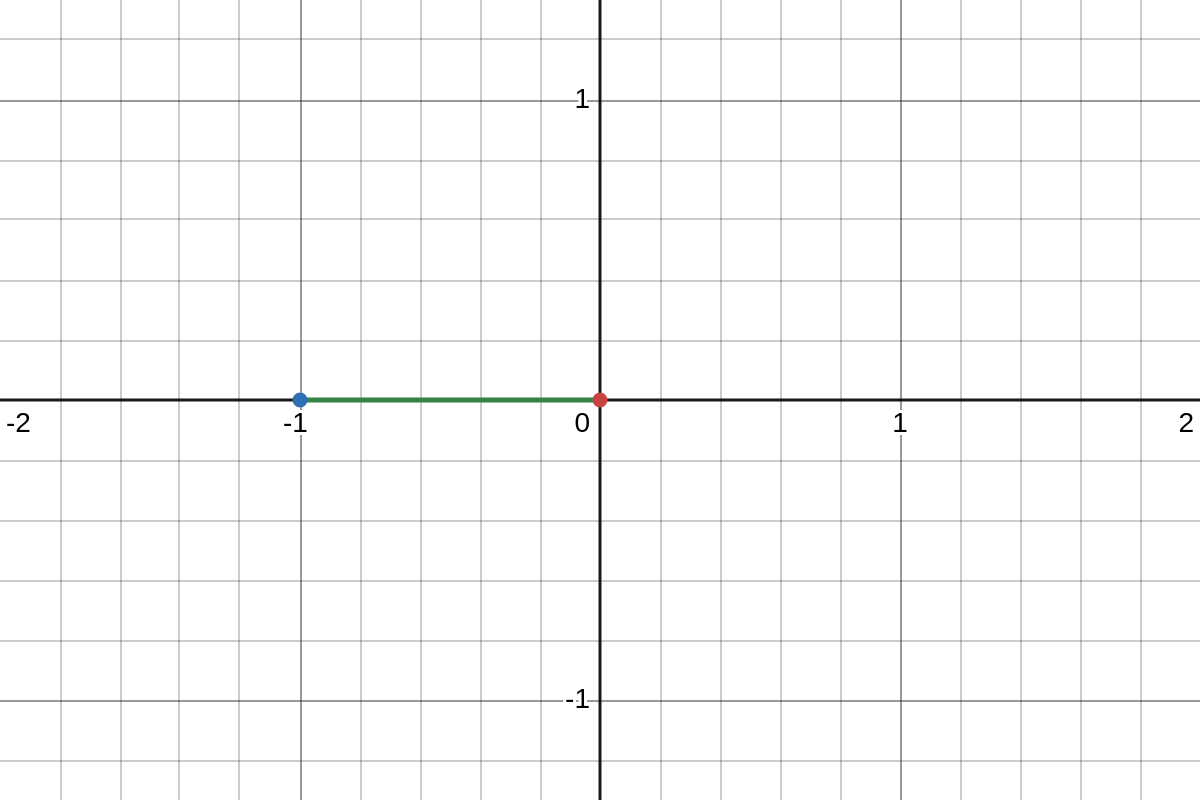
\includegraphics[scale=0.26]{../figures/locus_dr.png}
				\end{center}

				Abbiamo quindi preso tutti gli $s$ che hanno un numero \textbf{dispari} di poli a destra.

			\item Per $K < 0$ (luogo inverso) imponiamo invece la condizione:
				$$
				-\angle s (s + 1) =\pm 2 h \pi
				$$
				che è rispettata per tutti gli $s \in \mathbb{R}$ con $s \leq p_2$ o $s \geq p_1$.

				In questo caso si ha quindi la parte dell'asse reale:
				\begin{center}
					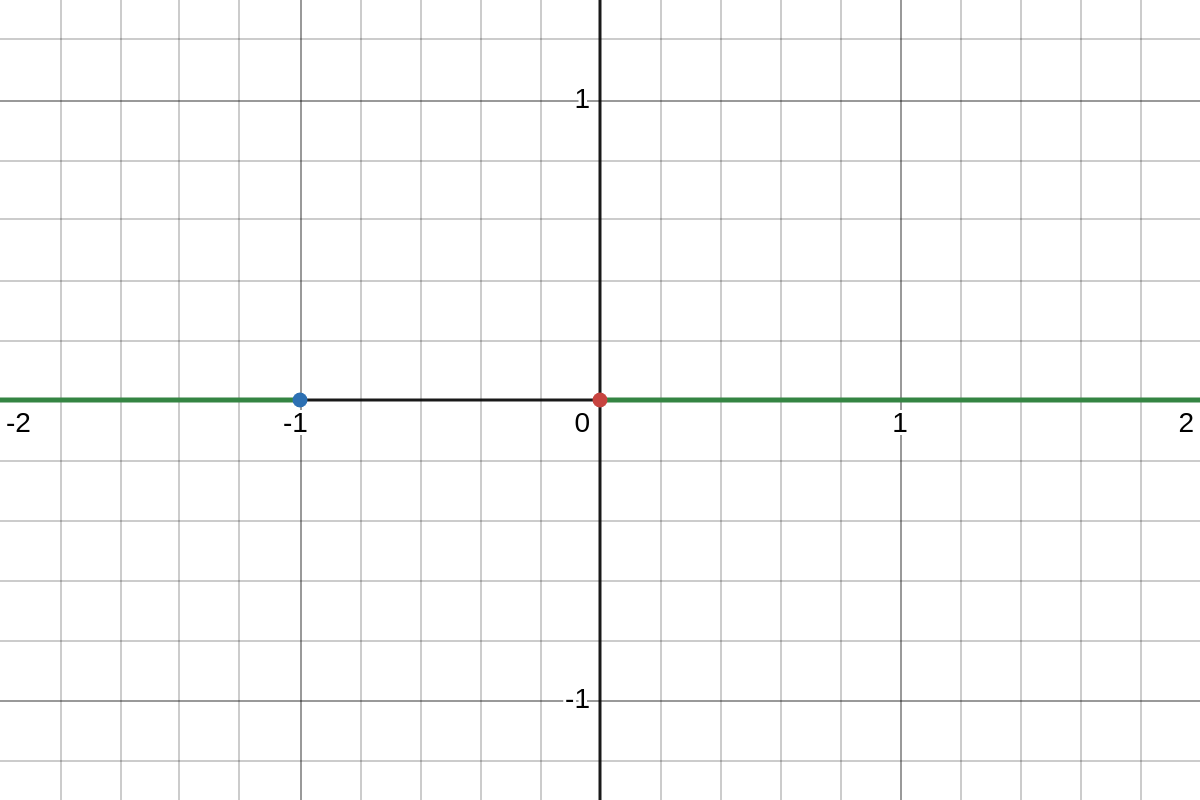
\includegraphics[scale=0.26]{../figures/locus_ir.png}
				\end{center}

				Abbiamo quindi preso tutti gli $s$ che hanno un numero \textbf{pari} di poli a destra.
		\end{itemize}

	\item
		La regola (5) afferma che il luogo delle radici è \textbf{simmetrico} rispetto all'\textit{asse reale}.
		Questo deriva direttamnente dal fatto che l'equazione caratteristica è reale, quindi ammetterà soluzioni reali o complesse coniugate.

		Vediamo quindi che dalla regola (2) rispetto agli angoli, tutto l'asse del segmento del luogo diretto sarà parte del luogo, in quanto avremo due angoli $\phi_1$ e $\phi_2$ ai poli fra di loro complementari (è questo proprio il caso che abbiamo preso ad esempio della regola (2)).
		In particolare potremmo dire, dati $\phi_1$ e $\phi_2$ complementari:
		$$
		-(\phi_1 + \phi_2) -(\phi_1 + (\pi - \phi_1)) = -\pi \pm 2 h \pi
		$$
		che chiaramente è rispettato per $h = 0$ (i meno vengono dal fatto che prendiamo poli al denominatore).

		Potremo quindi estendere il luogo diretto a (dove nel grafico si sono disegnati anche gli angoli complementari):
		\begin{center}
			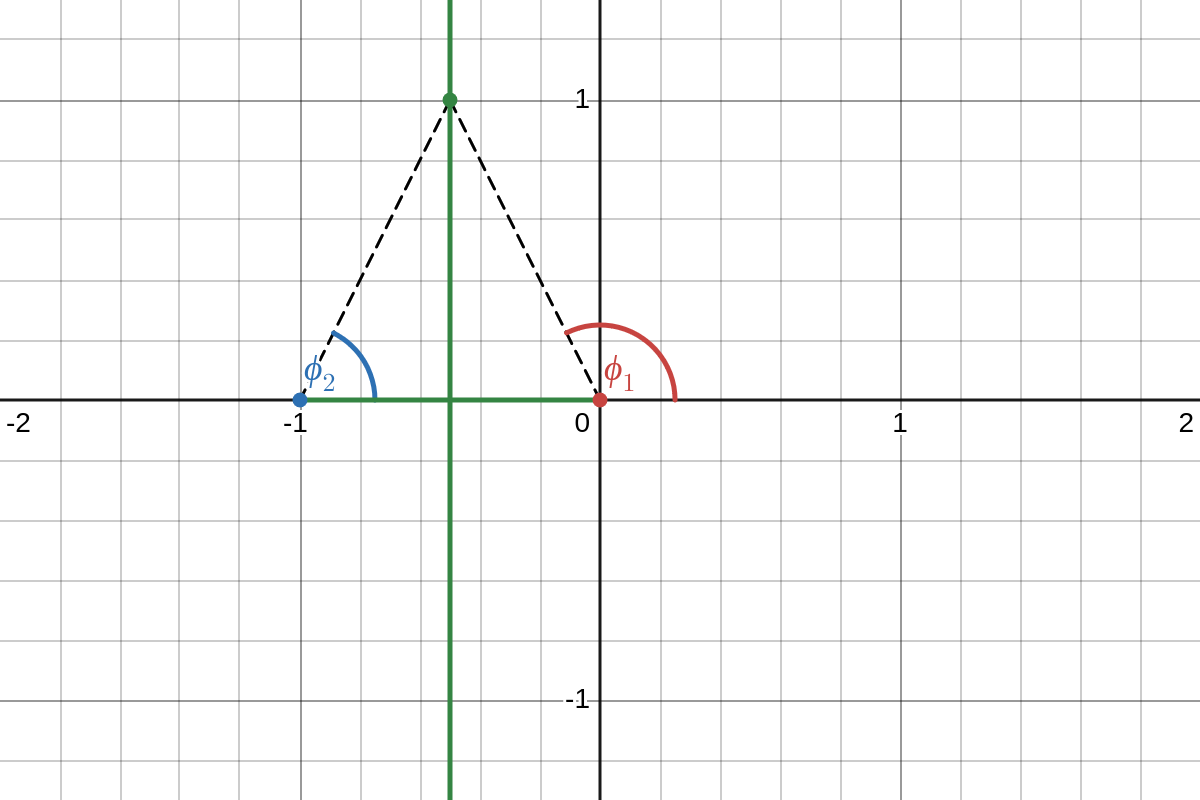
\includegraphics[scale=0.26]{../figures/locus_dc.png}
		\end{center}
		
		Notiamo che in ogni caso i rami sia del luogo diretto che del luogo inverso sono 2, come dalla regola (1).
\end{enumerate}

\end{document}


\documentclass[a4paper,11pt]{article}
\usepackage[a4paper, margin=8em]{geometry}

% usa i pacchetti per la scrittura in italiano
\usepackage[french,italian]{babel}
\usepackage[T1]{fontenc}
\usepackage[utf8]{inputenc}
\frenchspacing 

% usa i pacchetti per la formattazione matematica
\usepackage{amsmath, amssymb, amsthm, amsfonts}

% usa altri pacchetti
\usepackage{gensymb}
\usepackage{hyperref}
\usepackage{standalone}

% imposta il titolo
\title{Appunti Fondamenti di Automatica}
\author{Luca Seggiani}
\date{2025}

% disegni
\usepackage{pgfplots}
\pgfplotsset{width=10cm,compat=1.9}

% imposta lo stile
% usa helvetica
\usepackage[scaled]{helvet}
% usa palatino
\usepackage{palatino}
% usa un font monospazio guardabile
\usepackage{lmodern}

% tikz in sans
\tikzset{every picture/.style={/utils/exec={\sffamily}}}

\renewcommand{\rmdefault}{ppl}
\renewcommand{\sfdefault}{phv}
\renewcommand{\ttdefault}{lmtt}

% circuiti
\usepackage{circuitikz}
\usetikzlibrary{babel}

% disponi il titolo
\makeatletter
\renewcommand{\maketitle} {
	\begin{center} 
		\begin{minipage}[t]{.8\textwidth}
			\textsf{\huge\bfseries \@title} 
		\end{minipage}%
		\begin{minipage}[t]{.2\textwidth}
			\raggedleft \vspace{-1.65em}
			\textsf{\small \@author} \vfill
			\textsf{\small \@date}
		\end{minipage}
		\par
	\end{center}

	\thispagestyle{empty}
	\pagestyle{fancy}
}
\makeatother

% disponi teoremi
\usepackage{tcolorbox}
\newtcolorbox[auto counter, number within=section]{theorem}[2][]{%
	colback=blue!10, 
	colframe=blue!40!black, 
	sharp corners=northwest,
	fonttitle=\sffamily\bfseries, 
	title=Teorema~\thetcbcounter: #2, 
	#1
}

% disponi definizioni
\newtcolorbox[auto counter, number within=section]{definition}[2][]{%
	colback=red!10,
	colframe=red!40!black,
	sharp corners=northwest,
	fonttitle=\sffamily\bfseries,
	title=Definizione~\thetcbcounter: #2,
	#1
}

% disponi problemi
\newtcolorbox[auto counter, number within=section]{problem}[2][]{%
	colback=green!10,
	colframe=green!40!black,
	sharp corners=northwest,
	fonttitle=\sffamily\bfseries,
	title=Problema~\thetcbcounter: #2,
	#1
}

% disponi codice
\usepackage{listings}
\usepackage[table]{xcolor}

\lstdefinestyle{codestyle}{
	backgroundcolor=\color{black!5}, 
	commentstyle=\color{codegreen},
	keywordstyle=\bfseries\color{magenta},
	numberstyle=\sffamily\tiny\color{black!60},
	stringstyle=\color{green!50!black},
	basicstyle=\ttfamily\footnotesize,
	breakatwhitespace=false,         
	breaklines=true,                 
	captionpos=b,                    
	keepspaces=true,                 
	numbers=left,                    
	numbersep=5pt,                  
	showspaces=false,                
	showstringspaces=false,
	showtabs=false,                  
	tabsize=2
}

\lstdefinestyle{shellstyle}{
	backgroundcolor=\color{black!5}, 
	basicstyle=\ttfamily\footnotesize\color{black}, 
	commentstyle=\color{black}, 
	keywordstyle=\color{black},
	numberstyle=\color{black!5},
	stringstyle=\color{black}, 
	showspaces=false,
	showstringspaces=false, 
	showtabs=false, 
	tabsize=2, 
	numbers=none, 
	breaklines=true
}

\lstdefinelanguage{javascript}{
	keywords={typeof, new, true, false, catch, function, return, null, catch, switch, var, if, in, while, do, else, case, break},
	keywordstyle=\color{blue}\bfseries,
	ndkeywords={class, export, boolean, throw, implements, import, this},
	ndkeywordstyle=\color{darkgray}\bfseries,
	identifierstyle=\color{black},
	sensitive=false,
	comment=[l]{//},
	morecomment=[s]{/*}{*/},
	commentstyle=\color{purple}\ttfamily,
	stringstyle=\color{red}\ttfamily,
	morestring=[b]',
	morestring=[b]"
}

% disponi sezioni
\usepackage{titlesec}

\titleformat{\section}
{\sffamily\Large\bfseries} 
{\thesection}{1em}{} 
\titleformat{\subsection}
{\sffamily\large\bfseries}   
{\thesubsection}{1em}{} 
\titleformat{\subsubsection}
{\sffamily\normalsize\bfseries} 
{\thesubsubsection}{1em}{}

% disponi alberi
\usepackage{forest}

\forestset{
	rectstyle/.style={
		for tree={rectangle,draw,font=\large\sffamily}
	},
	roundstyle/.style={
		for tree={circle,draw,font=\large}
	}
}

% disponi algoritmi
\usepackage{algorithm}
\usepackage{algorithmic}
\makeatletter
\renewcommand{\ALG@name}{Algoritmo}
\makeatother

% disponi numeri di pagina
\usepackage{fancyhdr}
\fancyhf{} 
\fancyfoot[L]{\sffamily{\thepage}}

\makeatletter
\fancyhead[L]{\raisebox{1ex}[0pt][0pt]{\sffamily{\@title \ \@date}}} 
\fancyhead[R]{\raisebox{1ex}[0pt][0pt]{\sffamily{\@author}}}
\makeatother

\begin{document}

% sezione (data)
\section{Lezione del 16-04-25}

% stili pagina
\thispagestyle{empty}
\pagestyle{fancy}

% testo
Riprendiamo il discorso sul luogo delle radici, con maggiore attenzione su come \textit{tarare} (ottenere informazioni riguardo al modulo) i punti $s$.

\subsubsection{Taratura del luogo delle radici}
Abbiamo visto nella scorsa lezione come applicando la \textit{condizione di fase} possiamo tracciare tutto il luogo delle radici, diretto ed inverso.
Abbiamo poi introdotto come l'altra condizione, la \textit{condizione di modulo}, può essere usata per ottenere il modulo corrispondente ad un punto $s_i$ che già sappiamo appartenere al luogo delle radici.

Questa era quindi la condizione, che valutiamo nel punto $s_i$:
$$
\left| \frac{n(s)}{d(s)} \right| = \frac{1}{|K|} \xrightarrow{s_i} |K| \big|_{s = s_i} = \left| \frac{d(s_i)}{n(s_i)} \right|
$$

Riprendiamo l'esempio della scorsa lezione, che era:
$$
K \cdot G(s) = \frac{K}{s (s + 1)}
$$

Avremo quindi, applicando la condizione di modulo:
$$
|K| \big|_{s = s_i} = \frac{|s_i (s_i + 1)|}{|1|}
$$

Prendiamo ad esempio il punto che sta all'intersezione fra i due rami che avevamo individuato nel luogo diretto, cioè $s_i = -\frac{1}{2}$.
In questo caso avremo che il modulo di $K$ è:
$$
|K| \Big|_{s_i = -\frac{1}{2}} = \frac{\left|-\frac{1}{2} (-\frac{1}{2} + 1)\right|}{|1|} = \frac{1}{4}
$$

\subsection{Luogo delle radici complesse e coniugate}
Veniamo quindi a come tracciare i luoghi delle radici di sistemi del second'ordine.
Prendiamo quindi un nuovo esempio, che è la classica forma di Evans al secondo grado:
$$
G(s) = \frac{\omega_0^2}{s^2 + 2 \xi \omega_0 s + \omega_0 ^2}
$$
Le radici di questa sono note e valgono:
$$
p_{1, 2} = -\xi \omega_0 \pm \omega_0 j \sqrt{1 - \xi^2}
$$

\subsubsection{Valutazione di frequenza e smorzamento}

Vediamo quali informazioni sul sistema possiamo ottenere osservando le radici.

Prendendo quindi un punto all'origine nel piano di Gauss del luogo delle radici, e quindi l'angolo $\theta$ che la congiungente del punto e la radice a parte immaginaria positiva forma con l'asse immaginario, potremo dire:
$$
\omega_0 \sin(\theta) = \xi \omega_0 \implies \theta = \sin^{-1} (\xi) 
$$
cioè l'angolo $\theta$ va più o meno come lo smorzamento.

Di contro, considerando smorzamente fisso, si ha che la distanza dall'origine equivale alla frequenza naturale.
Infatti avremo che:
$$
\sqrt{ \xi^2 \omega_0^2 + \omega_0^2 (1 - \xi^2) } = \omega_0
$$

Riassumendo, quindi, si ha che:
\begin{itemize}
	\item $\xi = 0$: (\textit{smorzamento nullo}) i poli sono sull'asse immaginario;
	\item $\xi = 1$: (\textit{smorzamento perfetto})  i poli sono sul'asse reale e coincidenti;
	\item $0 < \xi < 1$: (\textit{sistema sottosmorzato}) i poli sono sulla semicirconferenza sinistra (uno in $\mathbb{C}^+$, l'altro in $\mathbb{C}^-$) di raggio $\omega_0$ centrata sull'origine.
	\item Il modulo delle radici corrisponde alla frequenza naturale $\omega_0$.
\end{itemize}

\subsubsection{Linee costanti}
Esistono diverse linee costanti che possiamo percorrere (cioè su cui possiamo posizionare i poli) in modo da mantenere certe caratteristiche del sistema costanti:
\begin{itemize}
	\item 
		Abbiamo quindi che percorrendo una retta passante per l'origine nella direzione negativa dell'asse complesso si ottiene una cosiddetta \textbf{linea di smorzamento costante}, cioè un insieme di regioni dove lo smorzamento resta costante e cambia invece (con l'aumentare della distanza dall'origine) la frequenza naturale. 

		Vediamo ad esempio il seguente grafico, dove a sinistra si mostrano le linee di smorzamento costante, e a sinistra le risposte all'impulso di alcuni dei sistemi che descrivono:
		\begin{center}
			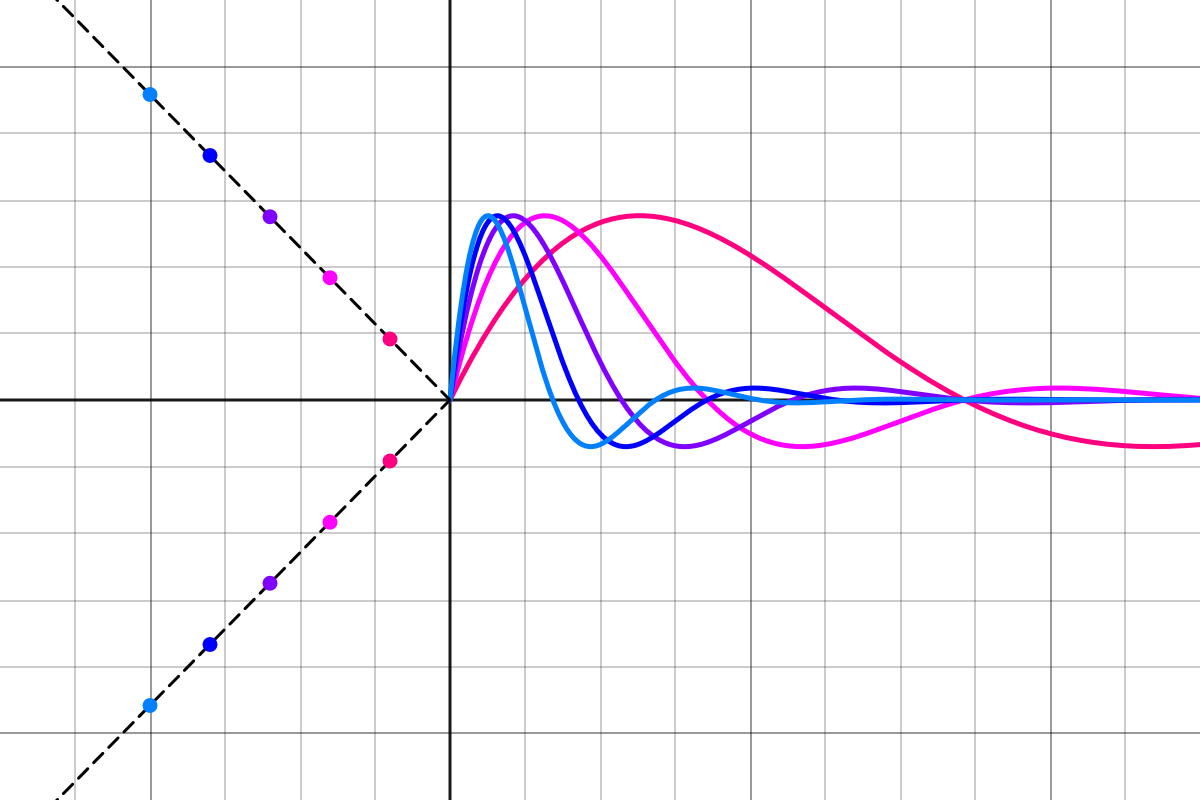
\includegraphics[scale=0.28]{../figures/fixed_damping.png}
		\end{center}
	\item
		Per mantenere costante il tempo di assestamento, invece, basta mantenere la componente reale dei poli costante, ergo si crea una cosiddetta \textbf{linea di tempo di assestamento costante} parallela all'asse immaginario. 

		\newpage

		Il grafico del tipo precedente per questa situazione è:
		\begin{center}
			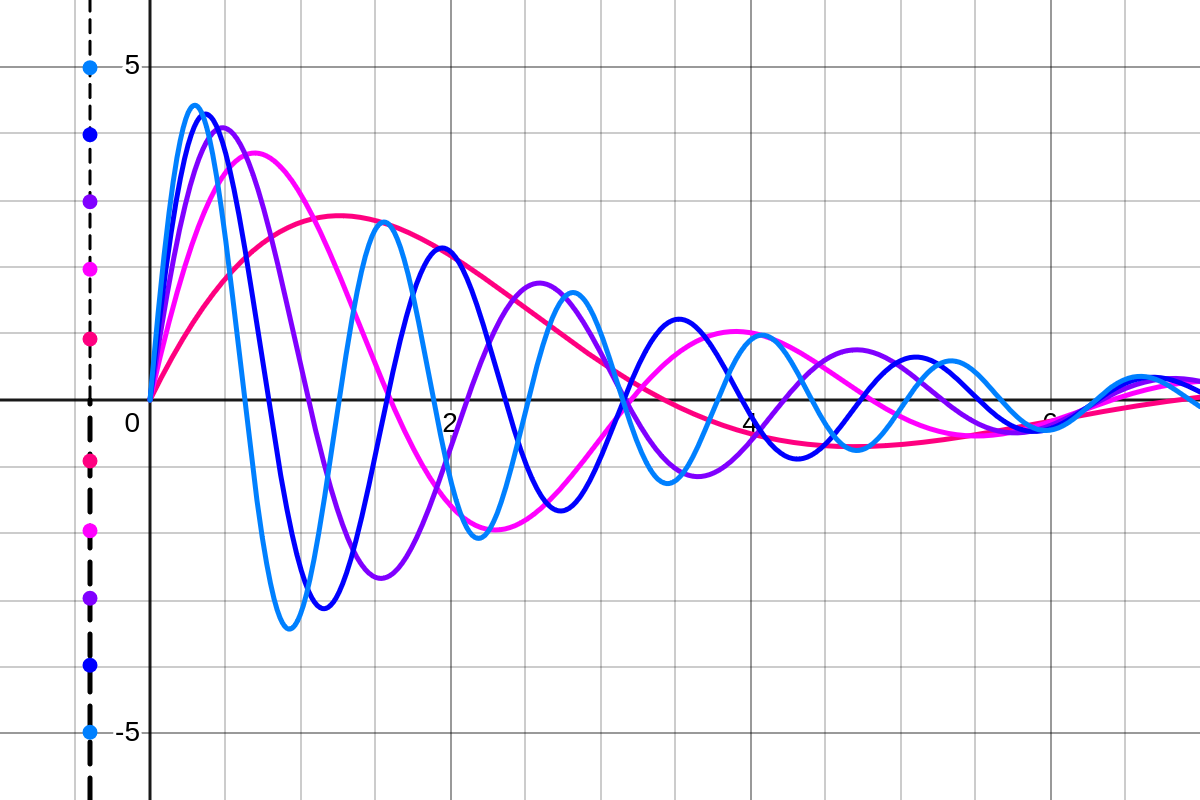
\includegraphics[scale=0.28]{../figures/fixed_time.png}
		\end{center}
	\item
		Per mantenere costante la pulsazione prendiamo circonferenze centrate sull'origine di raggio crescente, cioè cerchiamo una \textbf{circonferenza di pulsazione costante}.
		
		Il grafico del tipo precedente per questa situazione è:
		\begin{center}
			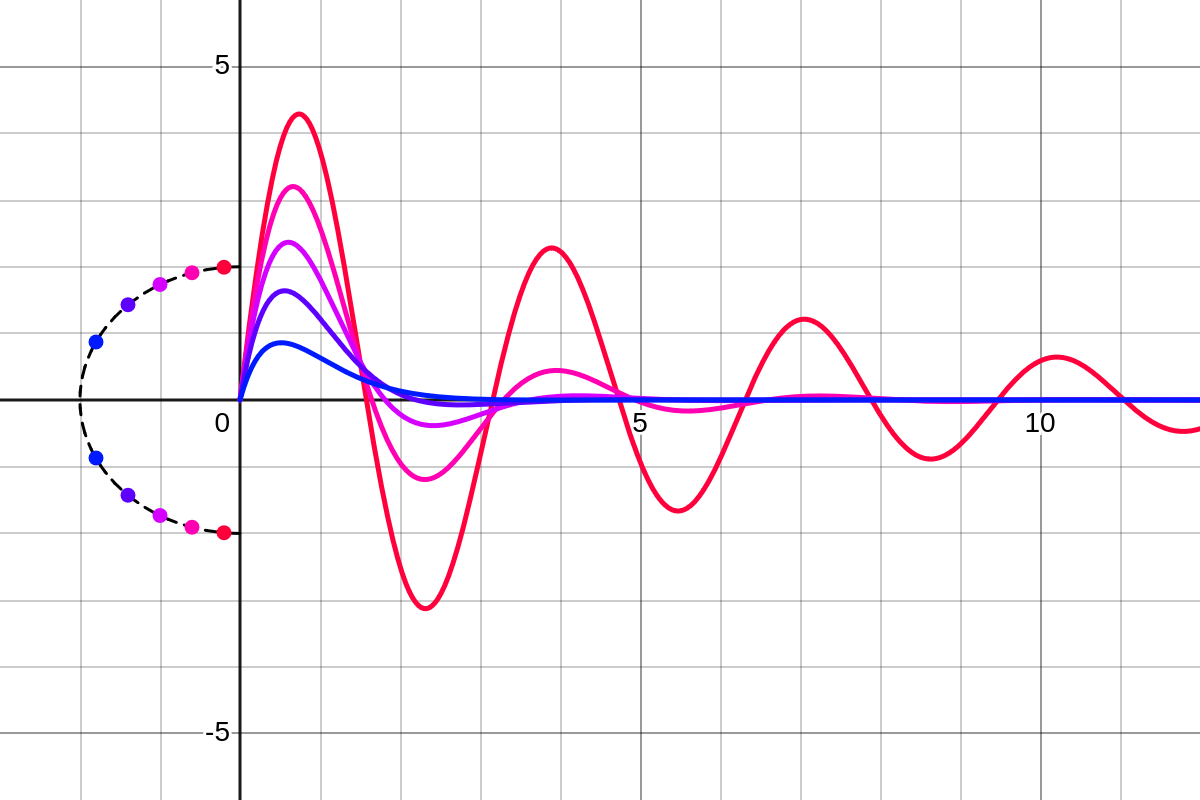
\includegraphics[scale=0.28]{../figures/fixed_pulse.png}
		\end{center}
\end{itemize}

\subsubsection{Regioni di vincolo}
Abbiamo parlato finora dei soli poli: vediamo di reintrodurre il sistema con controllore ($K$). 

Intanto possiamo vedere alcuni vincoli di progetto che potremmo avere sul comportamento desiderato:
\begin{itemize}
	\item 
		Potremmo volere che lo \textbf{smorzamento} che otterremo non sia mai minore di un certo valore. Saremo vincolati ad un cono di angolo $\theta$ con l'asse immaginario, che possiamo individuare sul piano di Argand-Gauss:
		\begin{center}
			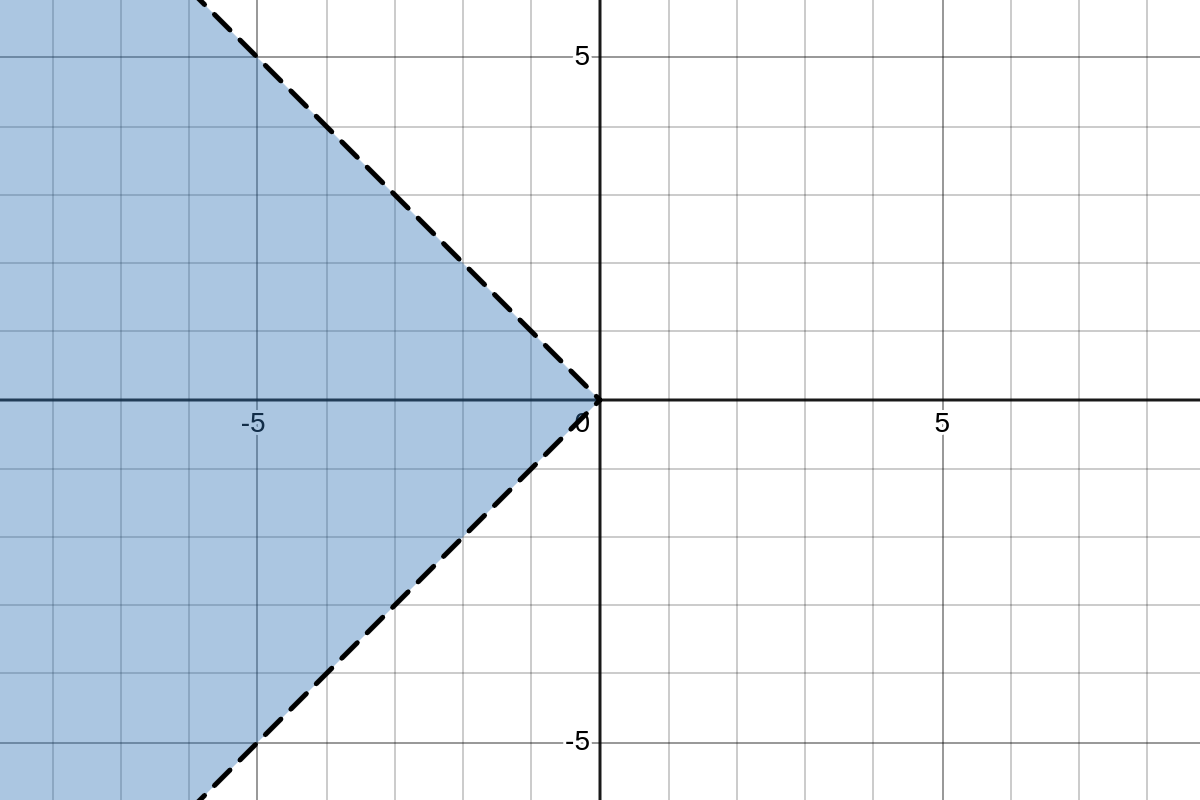
\includegraphics[scale=0.28]{../figures/fixed_damping_region.png}
		\end{center}

	\item
		Se volessimo invece \textbf{tempo di assestamento} sotto una certa soglia, vorremo trovarci a sinistra di una linea di tempo di assestamento costante, quindi in una regione di piano che il seguente aspetto:
		\begin{center}
			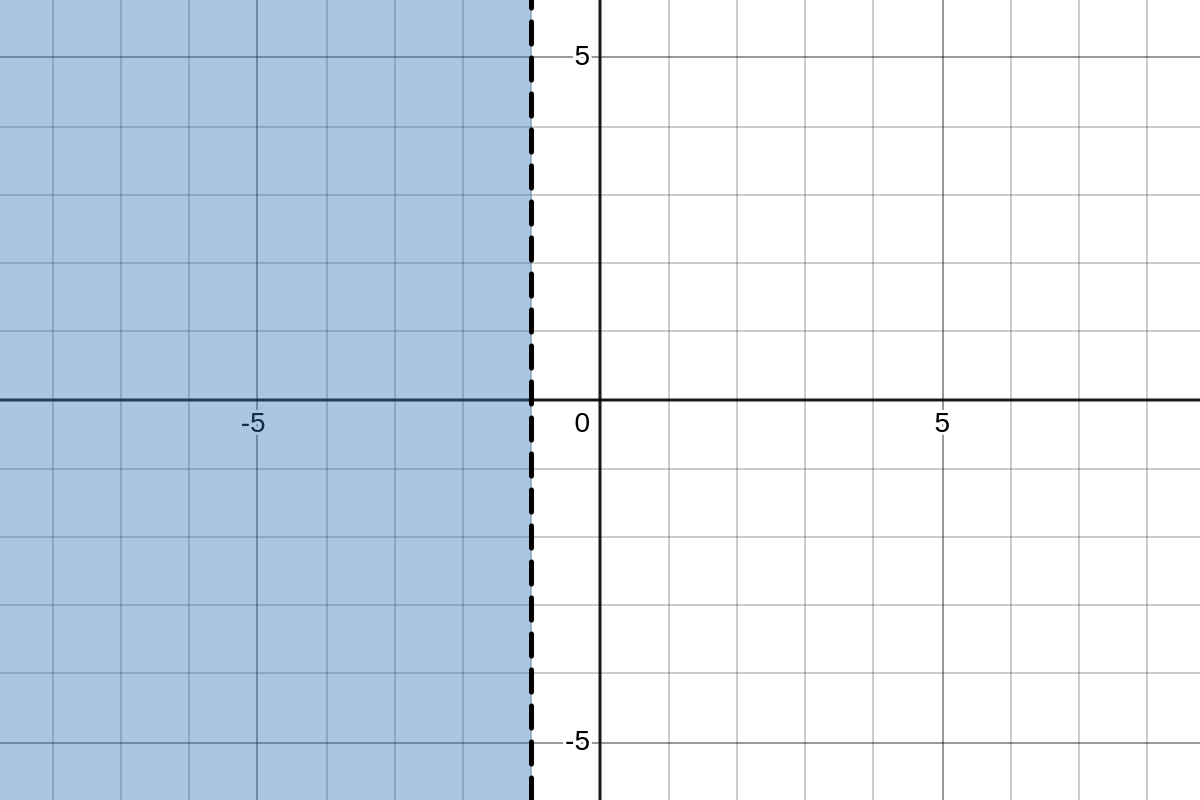
\includegraphics[scale=0.28]{../figures/fixed_time_region.png}
		\end{center}

	\item
		Infine potremmo voler vincolare la pulsazione naturale.
		In questo caso, direttamente dalla corrispondenza fra modulo e pulsazione naturale, ci vorremmo restiringere, ad esempio se si vuole pulsazione \textit{maggiore} (\textit{minore}) di una certa soglia, alla regione \textit{esterna} (\textit{interna}) ad una certa circonferenza di raggio equivalente alla soglia.
		
		\newpage

		Sul grafico:
		\begin{center}
			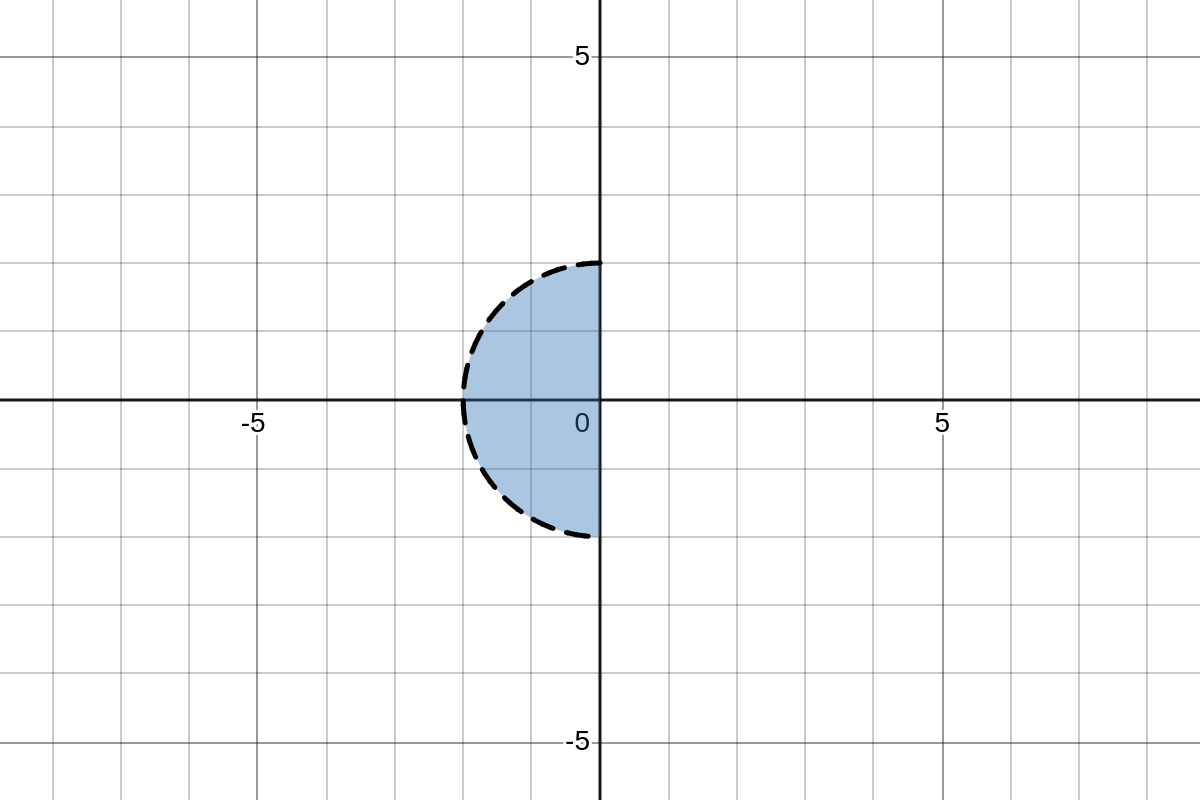
\includegraphics[scale=0.28]{../figures/fixed_pulse_region.png}
		\end{center}
\end{itemize}

L'insieme dei punti che rispettano tutti i vincoli si ha, a questo punto, semplicemente prendendo l'intersezione delle regioni individuate da ogni vincolo.

\subsubsection{Regole di tracciamento 2}
Vediamo quindi altre regole di tracciamento.

\begin{enumerate}
	\item[5.] La regola (5) riguarda le \textit{sovrapposizioni} di rami.
		In particolare, si ha che i rami non si sovrappongono mai, se non in punti singolari detti \textbf{punti multipli}, in quanto rappresentano \textit{radici multiple} del polinomio caratteristico.

		In un punto multiplo la radice multipla $s_i$ è soluzione di:
		\[
			\begin{cases}
				d(s_i) + Kn(s_i) = 0 \\
				d'(s_i) + K n'(s_i) = 0
			\end{cases}
		\]
		cioè dell'equazione caratteristica e della sua derivata.

		Inoltre, si nota che:
		$$
		\sum_{i = 1}^n \frac{1}{s_i - p_i} = \sum_{i = 1}^m \frac{1}{s_i - z_i}
		$$

		\par\medskip
		\noindent
		\textbf{\sffamily{Esempio}}

		Avevamo già visto questa situazione nel primo esempio di tracciamento, cioè:
		$$
		K \cdot G(s) = \frac{K}{s(s+1)}
		$$

		Vediamo infatti che risolvendo:
		$$
		\sum_{i = 1}^n \frac{1}{s - p_i} = \sum_{i = 1}^m \frac{1}{s - z_i}
		\implies \frac{1}{s} + \frac{1}{s + 1} = 0
		$$
		si ottiene la soluzione:
		$$
		s_i = -\frac{1}{2}
		$$
		che avevamo visto era esattamente un punto di intersezione fra rami (in particolare quello reale e immaginario nel luogo diretto).

	\item[6.] La regola (6) si concentra sul \textit{comportamento asintotico}, cioè su cosa accade per $K \rightarrow +\infty$.
		Avevamo anticipato che in questo caso i poli andavano al \textit{finito} (cioè agli zeri della funzione a ciclo aperto) o ad \textit{infinito}.
		Per quanto riguardava i poli ad infinito, avevamo detto che questi erano $n - m$ (cioè quelli che non andavano in zeri in ciclo aperto).
		Chiamiamo questo valore $v = n - m$, o \textit{differenza poli-zeri}.

		Avevamo dalla condizione di fase, cioè dalla regola (2), che i punti che appartengono al luogo delle radici sono quelli che rispettano:
		\[
			\begin{cases}
				\angle n(s) - \angle d(s) = -\pi \pm 2 h \pi, \quad K > 0 \\
				\angle n(s) - \angle d(s) = \pm 2 h \pi, \quad K < 0
			\end{cases}
		\]
		e cioè per cui la somma degli angoli agli zeri $\theta_i$ meno la somma degli angoli ai poli $\phi_i$ vale $-\pi$ per il luogo diretto, e $0$ per il luogo indiretto.
		Quando facciamo tendere $K$ ad infinito, si ha che gli angoli per tutti i poli e zeri diventano simili, cioè:
		$$
		\phi_i \approx \theta_i \approx \phi_\infty
		$$
		per cui potremo approssimare:
		$$
		\angle n(s) - \angle d(s) \approx \phi_{\infty} (m - n) = -\pi \pm 2 h \pi
		$$
		da cui la regola (nell'esempio per il luogo diretto).
		Notiamo che preferiamo usare $n - m$ invece di $m - n$ in quanto corrisponde direttamente con $v$, ma il risultato non cambia in quanto la condizione di fase funziona scambiando i segni a destra (se si ruota di $360^\circ$ su un cerchio si torna da dove si è partiti).

		Nota la differenza poli-zeri potremo quindi dire che:
		\begin{itemize}
			\item Esiste un \textbf{centro degli asintoti}, cioè il punto da cui iniziamo a tracciare gli asintoti, che sta sempre sull'asse reale ed è:
				$$
				\sigma = \frac{ \sum_{i = 1}^n p_i - \sum_{i = 1}^m z_i }{v}
				$$

			\item Gli asintoti dividono quindi il piano di Argand-Gauss in sezioni equiangole, cioè si hano gli \textbf{angoli di asintoto}:
				\[
					\phi_\text{asintoto} =
					\begin{cases}
						\frac{-\pi \pm 2 h \pi}{v}, \quad K > 0 \\
						\frac{2 h \pi}{v}, \quad K < 0 \\
					\end{cases}
				\]
		\end{itemize}

		\par\medskip
		\noindent
		\textbf{\sffamily{Esempio 1}}

		Vediamo la funzione di trasferimento di esempio:
		$$
		G(s) = \frac{1}{(s + 1)^3}
		$$
		in questo caso avremo il centro degli asintoti:
		$$
		\sigma = \frac{-1 -1 -1}{3} = -1
		$$
		e gli angoli di asintoto, rispettivamente per il luogo diretto e inverso:
		$$
		\phi_{asintoto} = \left\{ 60^\circ, 180^\circ, 300^\circ \right\}, \quad K > 0
		$$
		$$
		\phi_{asintoto} = \left\{ 0^\circ, 120^\circ, 240^\circ \right\}, \quad K < 0
		$$
		Notiamo che questi angoli non sono stati calcolati usando la formula, ma semplicemente notando di dover dividere, per $v = 3$, il piano di Argand-Gauss in regioni equiangole di angolo $120^\circ$.

	Sul grafico, questo sarà:
	\begin{center}
		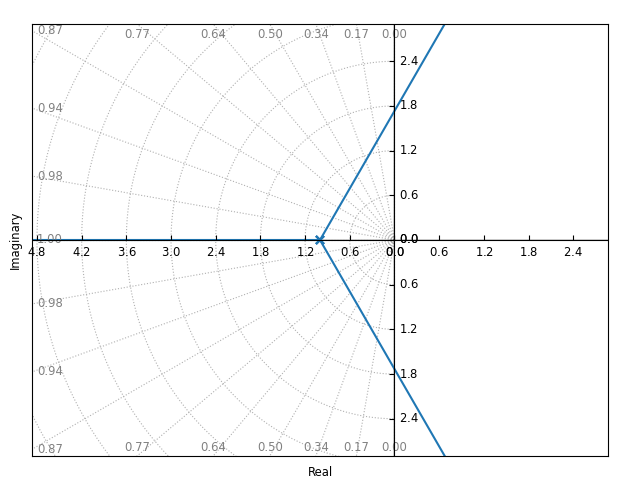
\includegraphics[scale=0.8]{../figures/rlocus/1331.png}
	\end{center}

		\par\medskip
		\noindent
		\textbf{\sffamily{Esempio 2}}

		Vediamo un'altro esempio, attraverso la funzione di trasferimento:
		$$
		G(s) = \frac{1}{s(s + 1)(s + 2)}
		$$
		In questo caso l'equazione caratteristica sarà:
		$$
		1 + K \cdot G(s) = s ( s + 1) ( s + 2) + K = s^3 + 3s^2 + 2s + K = 0
		$$

		Potrebbe interessarci valutare la stablità.
		In questo caso potremmo sfruttare il \textit{criterio di Routh}:
		\begin{table}[H]
			\center 
			\begin{tabular} { c | c c}
				$3$ & $1$ & $2$ \\
				$2$ & $3$ & $K$ \\
				$1$ & $\frac{6 - K}{3}$ & $0$ \\
				$0$ & $K$
			\end{tabular}
		\end{table}
		da cui le $K$ critiche $K_{CR1} = 0$ e $K_{CR2} = 6$, e quindi sistema stabile per $0 < K < 6$.

		Proseguiamo col tracciamento.
		Avremo che i poli sono $p_1 = -2$, $p_2 = -1$ e $p_3 = 0$
		Dalla regola (4), quindi, apparterranno al luogo diretto i punti in $(-\infty, -2]$, e i punti in $[-1, 0]$.

		Avremo $v = n - m = 3$ (non ci sono zeri), e quindi 3 asintoti (di cui uno è quello reale).
		Vorremo gli angoli di asintoto (sempre in luogo diretto):
		$$
		\phi_\text{asintoto} = \left\{ 60^\circ, 180^\circ, 300^\circ \right\}
		$$
		e il centro degli asintoti:
		$$
		\sigma = \frac{0 -1 -2}{3} = -1
		$$
		cioè sul piano complesso ci saranno due asintoti che si staccano da $-1$ e proseguono formando angoli di $60^\circ$ e $-60^\circ$ con l'asse reale. 

	Sul grafico, questo sarà:
	\begin{center}
		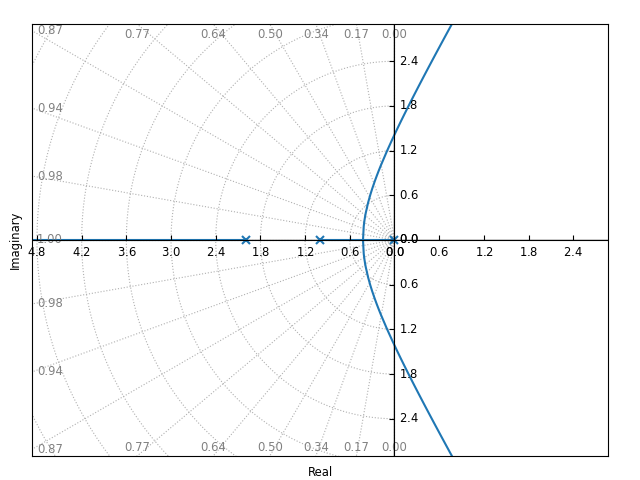
\includegraphics[scale=0.8]{../figures/rlocus/1320.png}
	\end{center}
	potremmo chiederci il valore del punto di intersezione fra i due rami.
	Ricordiamo allora la regola (5), per cui le radici doppie soddisfano:
	$$
	\sum_{i = 1}^n \frac{1}{s_i - p_i} = \sum_{i = 1}^m \frac{1}{s_i - z_i}
	$$
	che in questo caso significa:
	$$
	\frac{1}{s} + \frac{1}{s + 1} + \frac{1}{s + 2} = 0 \implies (s + 1) (s + 2) + s (s + 2) + s (s + 1) = 3s^2 + 6s + 2 = 0
	$$
	da cui le soluzioni:
	$$
		r_1 = \frac{-6 - \sqrt{12}}{6} \approx -1.577, \quad r_2 = \frac{-6 + \sqrt{12}}{6} \approx -0.4226
	$$
	dal grafico, si nota che il punto che cerchiamo dovrà essere compreso fra $-1$ e $0$, per cui prendiamo la seconda soluzione.

		\par\medskip
		\noindent
		\textbf{\sffamily{Esempio 3}}

		Prendiamo il caso di avere 2 poli coincidenti ed uno zero finito.
		In questo caso il luogo delle radici è una circonferenza centrata sullo zero.
		Questo si verifica dalla condizione di fase:
		$$
		\alpha - 2 \beta = - \pi \pm 2 h \pi
		$$
		Vogliamo dimostrare che questo vale su qualsiasi punto di una circonferenza centrata sullo zero e di raggio uguale alla differenza fra poli e zeri.
		Per questo prendiamo il disegno:
		\begin{center}
			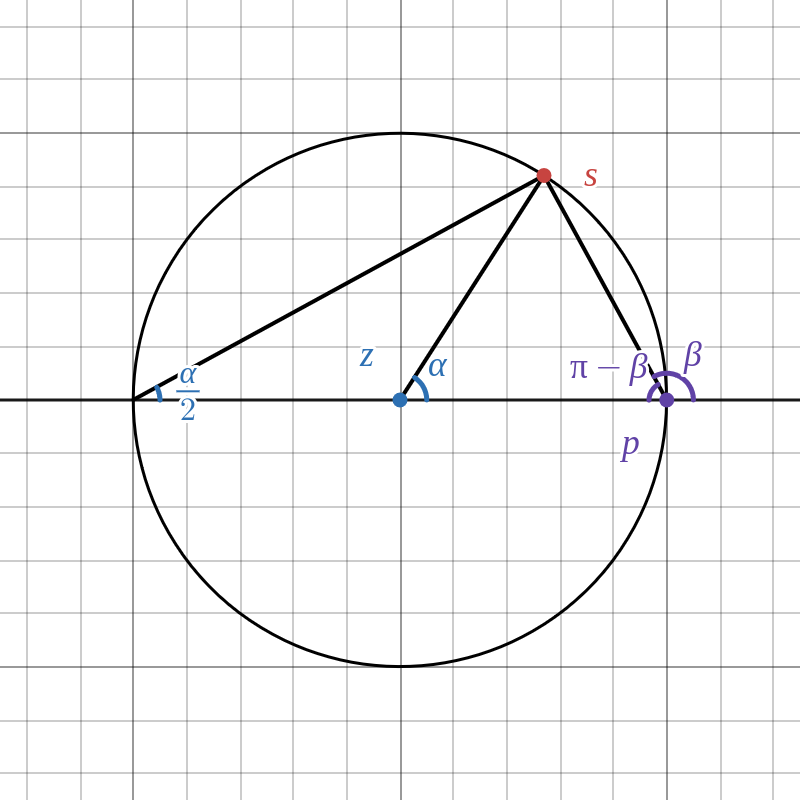
\includegraphics[scale=0.28]{../figures/rlocus_circ.png}
		\end{center}
		Osservando gli angoli si nota che deve valere:
		$$
		\frac{\alpha}{2} + (\pi - \beta) = \frac{\pi}{2} \, \Rightarrow \, \frac{\alpha}{2} - \beta = \frac{\pi}{2} - \pi \, \Rightarrow \, \alpha - 2 \beta = -\pi
		$$
		cioè la relazione, vera per ogni punto $s$ sulla circonferenza cercata, è equivalente alla condizione di fase per $h = 0$.

	\newpage

		Avremo quindi che i due poli, se sono reali, sono obbligatoriamente sovrapposti e tracciano il luogo:
	\begin{center}
		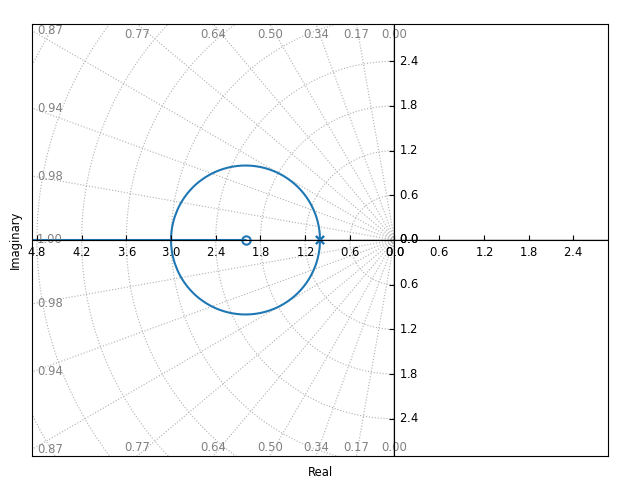
\includegraphics[scale=0.8]{../figures/rlocus/circ_full.png}
	\end{center}

	Il risultato si generalizza a funzioni di trasferimento qualsiasi con 2 poli complessi coniugati e uno zero finito.
	In questo caso il luogo è sempre una circonferenza vincolata sullo zero, dove i poli ne vincolano gli estremi:
	\begin{center}
		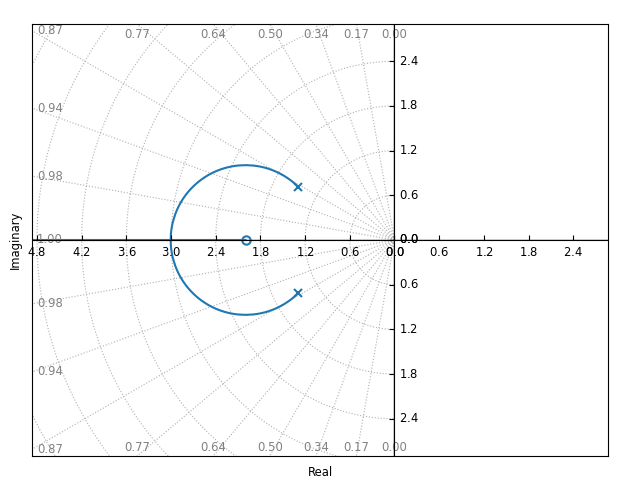
\includegraphics[scale=0.8]{../figures/rlocus/circ_cut.png}
	\end{center}

	\item[7.] La regola (7) riguarda gli angoli di partenza dei rami uscenti dai poli.
		Per ricavare una regola generale riprendiamo la condizione di fase:
		\[
			\begin{cases}
				\angle n(s) - \angle d(s) = -\pi \pm 2 h \pi, \quad K > 0 \\
				\angle n(s) - \angle d(s) = \pm 2 h \pi, \quad K < 0
			\end{cases}
		\]
		E notiamo che preso un polo particolare in $p^*$, ad esempio riguardo al luogo diretto, si avrà che l'angolo di uscita $\phi^*$ è:
		$$
		\angle n(s) - \angle d^*(s) \Big|_{s = p^*} - \phi^* = -\pi \implies \phi^* = \pi + \angle n(s) - \angle d^*(s) \Big|_{s = p^*}
		$$
		dove $d^*(s)$ è il denominatore rimosso il polo $p^*$ preso in considerazione.

		Potremo quindi usare questa formula generale per calcolare l'angolo di uscita dei rami dai poli.
		Da questo ricaviamo fra l'altro che i rami uscenti dai poli con molteplicità $> 1$ dividono il piano in parti equiangole e simmetriche rispetto all'asse reale.
		Infine, nessuno ci nega di applicare la stessa legge agli angoli di arrivo negli zeri (quindi di capire gli angoli finali dei rami che terminano \textit{al finito}).
		Vedremo questa situazione particolare nella regola (8).

		\par\medskip
		\noindent
		\textbf{\sffamily{Esempio}}

		Calcoliamo gli angoli di partenza dai poli della funzione di trasferimento:
		$$
		G(s) = \frac{s + 5}{s (s^2 + 6s + 109)}
		$$
		
		Partiamo col trovare i poli, di cui il polo banale $p_1 = 0$ e i poli complessi coniugati:
		$$
		p_{2, 3} = \frac{-6 \pm \sqrt{400}}{2} = -3 \pm 10i
		$$
		
		Abbiamo quindi i poli:
		$$
			p_1 = 0, \quad p_2 = -3 + 10 i, \quad p_3 = -3 - 10 i
		$$
		e la funzione di trasferimento fattorizzata:
		$$
		G(s) = \frac{s + 5}{s(s + 3 - 10i)(s + 3 + 10i)}
		$$

		Calcoliamo allora gli angoli veri e propri per ogni polo, applicando la legge appena trovata:
		\begin{itemize}
			\item Per il polo $p_1$ si ha cancellazione dei termini complessi:
		$$
		\phi_1 = \pi + \angle n(s) - \angle d^1(s) \Big|_{s = 0} = \pi + \angle 5 - \angle(3 - 10i) - \angle (3 + 10 i) =180^\circ
		$$
		e quindi il ramo è diretto a sinistra nell'asse reale, come ci aspettavamo dalla regola (4). 
	\item Per il polo $p_2$ prendiamo: 
		$$
		\phi_2 = \pi + \angle n(s) - \angle d^2(s) \Big|_{s = -3 + 10i} = \pi + \angle (-2 + 10i) - \angle (-3 + 10i) - \angle 20 i
		$$
		$$
		= 180^\circ + 78.7^\circ - 106.7^\circ - 90^\circ = 62^\circ
		$$
	\item Per il polo $p_3$ ci aspettiamo di trovare l'opposto di $\phi_2$, in quanto dalla regola (5) il luogo dovrà essere simmetrico rispetto all'asse reale.
		Facciamo comunqe il calcolo esplicito per completezza:
		$$
		\phi_3 = \pi + \angle n(s) - \angle d^3(s) \Big|_{s = -3 - 10i} = \pi + \angle (2 - 10i) - \angle (-3 - 10i) - \angle -20 i
		$$
		$$
		= 180^\circ - 78.7^\circ + 106.7^\circ + 90^\circ = -62^\circ
		$$
		che conferma quanto ci aspettavamo.
		\end{itemize}

		Vediamo quindi il grafico del luogo diretto:
		\begin{center}
			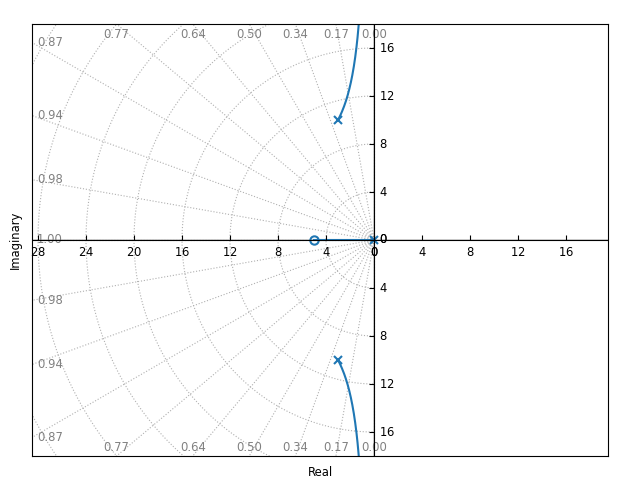
\includegraphics[scale=0.8]{../figures/rlocus/15_151090.png}
		\end{center}
\end{enumerate}

\end{document}


\documentclass[a4paper,11pt]{article}
\usepackage[a4paper, margin=8em]{geometry}

% usa i pacchetti per la scrittura in italiano
\usepackage[french,italian]{babel}
\usepackage[T1]{fontenc}
\usepackage[utf8]{inputenc}
\frenchspacing 

% usa i pacchetti per la formattazione matematica
\usepackage{amsmath, amssymb, amsthm, amsfonts}

% usa altri pacchetti
\usepackage{gensymb}
\usepackage{hyperref}
\usepackage{standalone}

% imposta il titolo
\title{Appunti Fondamenti di Automatica}
\author{Luca Seggiani}
\date{2025}

% disegni
\usepackage{pgfplots}
\pgfplotsset{width=10cm,compat=1.9}

% imposta lo stile
% usa helvetica
\usepackage[scaled]{helvet}
% usa palatino
\usepackage{palatino}
% usa un font monospazio guardabile
\usepackage{lmodern}

% tikz in sans
\tikzset{every picture/.style={/utils/exec={\sffamily}}}

\renewcommand{\rmdefault}{ppl}
\renewcommand{\sfdefault}{phv}
\renewcommand{\ttdefault}{lmtt}

% circuiti
\usepackage{circuitikz}
\usetikzlibrary{babel}

% disponi il titolo
\makeatletter
\renewcommand{\maketitle} {
	\begin{center} 
		\begin{minipage}[t]{.8\textwidth}
			\textsf{\huge\bfseries \@title} 
		\end{minipage}%
		\begin{minipage}[t]{.2\textwidth}
			\raggedleft \vspace{-1.65em}
			\textsf{\small \@author} \vfill
			\textsf{\small \@date}
		\end{minipage}
		\par
	\end{center}

	\thispagestyle{empty}
	\pagestyle{fancy}
}
\makeatother

% disponi teoremi
\usepackage{tcolorbox}
\newtcolorbox[auto counter, number within=section]{theorem}[2][]{%
	colback=blue!10, 
	colframe=blue!40!black, 
	sharp corners=northwest,
	fonttitle=\sffamily\bfseries, 
	title=Teorema~\thetcbcounter: #2, 
	#1
}

% disponi definizioni
\newtcolorbox[auto counter, number within=section]{definition}[2][]{%
	colback=red!10,
	colframe=red!40!black,
	sharp corners=northwest,
	fonttitle=\sffamily\bfseries,
	title=Definizione~\thetcbcounter: #2,
	#1
}

% disponi problemi
\newtcolorbox[auto counter, number within=section]{problem}[2][]{%
	colback=green!10,
	colframe=green!40!black,
	sharp corners=northwest,
	fonttitle=\sffamily\bfseries,
	title=Problema~\thetcbcounter: #2,
	#1
}

% disponi codice
\usepackage{listings}
\usepackage[table]{xcolor}

\lstdefinestyle{codestyle}{
	backgroundcolor=\color{black!5}, 
	commentstyle=\color{codegreen},
	keywordstyle=\bfseries\color{magenta},
	numberstyle=\sffamily\tiny\color{black!60},
	stringstyle=\color{green!50!black},
	basicstyle=\ttfamily\footnotesize,
	breakatwhitespace=false,         
	breaklines=true,                 
	captionpos=b,                    
	keepspaces=true,                 
	numbers=left,                    
	numbersep=5pt,                  
	showspaces=false,                
	showstringspaces=false,
	showtabs=false,                  
	tabsize=2
}

\lstdefinestyle{shellstyle}{
	backgroundcolor=\color{black!5}, 
	basicstyle=\ttfamily\footnotesize\color{black}, 
	commentstyle=\color{black}, 
	keywordstyle=\color{black},
	numberstyle=\color{black!5},
	stringstyle=\color{black}, 
	showspaces=false,
	showstringspaces=false, 
	showtabs=false, 
	tabsize=2, 
	numbers=none, 
	breaklines=true
}

\lstdefinelanguage{javascript}{
	keywords={typeof, new, true, false, catch, function, return, null, catch, switch, var, if, in, while, do, else, case, break},
	keywordstyle=\color{blue}\bfseries,
	ndkeywords={class, export, boolean, throw, implements, import, this},
	ndkeywordstyle=\color{darkgray}\bfseries,
	identifierstyle=\color{black},
	sensitive=false,
	comment=[l]{//},
	morecomment=[s]{/*}{*/},
	commentstyle=\color{purple}\ttfamily,
	stringstyle=\color{red}\ttfamily,
	morestring=[b]',
	morestring=[b]"
}

% disponi sezioni
\usepackage{titlesec}

\titleformat{\section}
{\sffamily\Large\bfseries} 
{\thesection}{1em}{} 
\titleformat{\subsection}
{\sffamily\large\bfseries}   
{\thesubsection}{1em}{} 
\titleformat{\subsubsection}
{\sffamily\normalsize\bfseries} 
{\thesubsubsection}{1em}{}

% disponi alberi
\usepackage{forest}

\forestset{
	rectstyle/.style={
		for tree={rectangle,draw,font=\large\sffamily}
	},
	roundstyle/.style={
		for tree={circle,draw,font=\large}
	}
}

% disponi algoritmi
\usepackage{algorithm}
\usepackage{algorithmic}
\makeatletter
\renewcommand{\ALG@name}{Algoritmo}
\makeatother

% disponi numeri di pagina
\usepackage{fancyhdr}
\fancyhf{} 
\fancyfoot[L]{\sffamily{\thepage}}

\makeatletter
\fancyhead[L]{\raisebox{1ex}[0pt][0pt]{\sffamily{\@title \ \@date}}} 
\fancyhead[R]{\raisebox{1ex}[0pt][0pt]{\sffamily{\@author}}}
\makeatother

\begin{document}

% sezione (data)
\section{Lezione del 24-04-25}

% stili pagina
\thispagestyle{empty}
\pagestyle{fancy}

% testo
Riprendiamo la trattazione delle regole di tracciamento del luogo delle radici.

\subsubsection{Regole di tracciamento 3}
\begin{enumerate}
	\item[8.] Come anticipato, la regola (8) è in qualche modo duale alla (7), e riguarda gli angoli dei rami entranti negli zeri.

		Riprendiamo la condizione di fase:
		\[
			\begin{cases}
				\angle n(s) - \angle d(s) = -\pi \pm 2 h \pi, \quad K > 0 \\
				\angle n(s) - \angle d(s) = \pm 2 h \pi, \quad K < 0
			\end{cases}
		\]
		E notiamo che preso uno zero particolare in $z^*$, ad esempio riguardo al luogo diretto, si avrà che l'angolo di entrata $\theta^*$ è:
		$$
		\angle n^*(s) + \theta^* - \angle d(s) \Big|_{s = z^*} = -\pi \implies \theta^* = -\pi + \angle d(s) - \angle n^*(s) \Big|_{s = z^*}
		$$
		dove $n^*(s)$ è il numeratore rimosso lo zero $z^*$ preso in considerazione.

		Potremo quindi usare questa formula generale per calcolare l'angolo di entrata dei rami negli zeri.
		Da questo ricaviamo fra l'altro che i rami entranti nei poli con molteplicità $> 1$ dividono il piano in parti equiangole e simmetriche rispetto all'asse reale.

		\par\medskip
		\noindent
		\textbf{\sffamily{Esempio}}
		
		Calcoliamo gli angoli di entrata negli zeri della funzione di trasferimento:
		$$
		G(s) = \frac{s^2 + 20s + 101}{s (s + 5)^3}
		$$
		Partiamo sempre col trovare zeri e poli, che saranno:
		$$
		z_{1, 2} = -10 \pm i, \quad p_1 = 0, \quad p_{2, 3, 4} = -5
		$$
		per cui potremo fattorizzare la funzione di trasferimento:
		$$
		G(s) = \frac{ (s + 10 - i)(s + 10 + i) }{ s (s + 5)^3 }
		$$

		Calcoliamo allora gli angoli veri e propri per ogni zero, applicando la legge appena trovata:
		\begin{itemize}
			\item Per lo zero $z_1$ si ha:
				$$
					\theta_1 = - \pi + \angle d(s) - \angle n^1(s) \Big|_{s = z_1} = -\pi + \angle(10 + i) + 3 \cdot \angle (-5 + i) - \angle  2i 
				$$
				$$
				= -180^\circ + 174.3^\circ + 506.07^\circ -90^\circ = 50.37^\circ
				$$
			\item Per lo zero $z_2$, complesso coniugato allo $z_1$, ci aspettiamo di ottenere l'opposto di $\theta_1$. Verifichiamo:
				$$
					\theta_2 = - \pi + \angle d(s) - \angle n^2(s) \Big|_{s = z_2} = -\pi + \angle(-10 - i) + 3 \cdot \angle (-5 - i) - \angle -2i 
				$$
				$$
				= -180^\circ - 174.3^\circ - 506.07^\circ +90^\circ = -50.37^\circ
				$$
		\end{itemize}

\end{enumerate}

\subsubsection{Riassunto sul luogo delle radici}
Abbiamo quindi che il luogo delle radici è una tecnica per determinare lo spostamento dei poli dal ciclo aperto al ciclo chiuso: inserito un controllore proporzionale di guadagno $K$, abbiamo ch al variare di $K$ i poli in ciclo chiuso cambiano posizione, appunto quelle che figurano nel luogo delle radici.

Il procedimento che seguiremo nel progetto dei controllori sarà quindi:
\begin{itemize}
	\item Fissare i poli/zeri del regolatore sulla base delle specifiche date;
	\item Variare $K$ per individuare il valore che fissa i \textit{poli dominanti} del sistema nella regione opportuna, sulla base delle specifiche, del piano complesso.
\end{itemize}

\end{document}


\documentclass[a4paper,11pt]{article}
\usepackage[a4paper, margin=8em]{geometry}

% usa i pacchetti per la scrittura in italiano
\usepackage[french,italian]{babel}
\usepackage[T1]{fontenc}
\usepackage[utf8]{inputenc}
\frenchspacing 

% usa i pacchetti per la formattazione matematica
\usepackage{amsmath, amssymb, amsthm, amsfonts}

% usa altri pacchetti
\usepackage{gensymb}
\usepackage{hyperref}
\usepackage{standalone}

% imposta il titolo
\title{Appunti Fondamenti di Automatica}
\author{Luca Seggiani}
\date{2025}

% disegni
\usepackage{pgfplots}
\pgfplotsset{width=10cm,compat=1.9}

% imposta lo stile
% usa helvetica
\usepackage[scaled]{helvet}
% usa palatino
\usepackage{palatino}
% usa un font monospazio guardabile
\usepackage{lmodern}

% tikz in sans
\tikzset{every picture/.style={/utils/exec={\sffamily}}}

\renewcommand{\rmdefault}{ppl}
\renewcommand{\sfdefault}{phv}
\renewcommand{\ttdefault}{lmtt}

% circuiti
\usepackage{circuitikz}
\usetikzlibrary{babel}

% disponi il titolo
\makeatletter
\renewcommand{\maketitle} {
	\begin{center} 
		\begin{minipage}[t]{.8\textwidth}
			\textsf{\huge\bfseries \@title} 
		\end{minipage}%
		\begin{minipage}[t]{.2\textwidth}
			\raggedleft \vspace{-1.65em}
			\textsf{\small \@author} \vfill
			\textsf{\small \@date}
		\end{minipage}
		\par
	\end{center}

	\thispagestyle{empty}
	\pagestyle{fancy}
}
\makeatother

% disponi teoremi
\usepackage{tcolorbox}
\newtcolorbox[auto counter, number within=section]{theorem}[2][]{%
	colback=blue!10, 
	colframe=blue!40!black, 
	sharp corners=northwest,
	fonttitle=\sffamily\bfseries, 
	title=Teorema~\thetcbcounter: #2, 
	#1
}

% disponi definizioni
\newtcolorbox[auto counter, number within=section]{definition}[2][]{%
	colback=red!10,
	colframe=red!40!black,
	sharp corners=northwest,
	fonttitle=\sffamily\bfseries,
	title=Definizione~\thetcbcounter: #2,
	#1
}

% disponi problemi
\newtcolorbox[auto counter, number within=section]{problem}[2][]{%
	colback=green!10,
	colframe=green!40!black,
	sharp corners=northwest,
	fonttitle=\sffamily\bfseries,
	title=Problema~\thetcbcounter: #2,
	#1
}

% disponi codice
\usepackage{listings}
\usepackage[table]{xcolor}

\lstdefinestyle{codestyle}{
	backgroundcolor=\color{black!5}, 
	commentstyle=\color{codegreen},
	keywordstyle=\bfseries\color{magenta},
	numberstyle=\sffamily\tiny\color{black!60},
	stringstyle=\color{green!50!black},
	basicstyle=\ttfamily\footnotesize,
	breakatwhitespace=false,         
	breaklines=true,                 
	captionpos=b,                    
	keepspaces=true,                 
	numbers=left,                    
	numbersep=5pt,                  
	showspaces=false,                
	showstringspaces=false,
	showtabs=false,                  
	tabsize=2
}

\lstdefinestyle{shellstyle}{
	backgroundcolor=\color{black!5}, 
	basicstyle=\ttfamily\footnotesize\color{black}, 
	commentstyle=\color{black}, 
	keywordstyle=\color{black},
	numberstyle=\color{black!5},
	stringstyle=\color{black}, 
	showspaces=false,
	showstringspaces=false, 
	showtabs=false, 
	tabsize=2, 
	numbers=none, 
	breaklines=true
}

\lstdefinelanguage{javascript}{
	keywords={typeof, new, true, false, catch, function, return, null, catch, switch, var, if, in, while, do, else, case, break},
	keywordstyle=\color{blue}\bfseries,
	ndkeywords={class, export, boolean, throw, implements, import, this},
	ndkeywordstyle=\color{darkgray}\bfseries,
	identifierstyle=\color{black},
	sensitive=false,
	comment=[l]{//},
	morecomment=[s]{/*}{*/},
	commentstyle=\color{purple}\ttfamily,
	stringstyle=\color{red}\ttfamily,
	morestring=[b]',
	morestring=[b]"
}

% disponi sezioni
\usepackage{titlesec}

\titleformat{\section}
{\sffamily\Large\bfseries} 
{\thesection}{1em}{} 
\titleformat{\subsection}
{\sffamily\large\bfseries}   
{\thesubsection}{1em}{} 
\titleformat{\subsubsection}
{\sffamily\normalsize\bfseries} 
{\thesubsubsection}{1em}{}

% disponi alberi
\usepackage{forest}

\forestset{
	rectstyle/.style={
		for tree={rectangle,draw,font=\large\sffamily}
	},
	roundstyle/.style={
		for tree={circle,draw,font=\large}
	}
}

% disponi algoritmi
\usepackage{algorithm}
\usepackage{algorithmic}
\makeatletter
\renewcommand{\ALG@name}{Algoritmo}
\makeatother

% disponi numeri di pagina
\usepackage{fancyhdr}
\fancyhf{} 
\fancyfoot[L]{\sffamily{\thepage}}

\makeatletter
\fancyhead[L]{\raisebox{1ex}[0pt][0pt]{\sffamily{\@title \ \@date}}} 
\fancyhead[R]{\raisebox{1ex}[0pt][0pt]{\sffamily{\@author}}}
\makeatother

\begin{document}

% sezione (data)
\section{Lezione del 28-04-25}

% stili pagina
\thispagestyle{empty}
\pagestyle{fancy}

% testo
\subsection{Diagrammi di Nyquist}
Vediamo quindi l'ultimo strumento che sfrutteremo per poi progettare i regolatori, cioè i \textbf{diagrammi di Nyquist}.
Questi rappresentano la forma polare della risposta in frequenza associata alla funzione di trasferimento di un sistema lineare $G(s)$.

Tracciare un diagramma di Nyquist significherà quindi tracciare una curva sul piano complesso paramaterizzata dalla pulsazione (o frequenza).

Avremo che:
\begin{itemize}
	\item L'asse delle ascisse riporta i valori di $\mathrm{Re}\left( G(j \omega) \right)$;
	\item L'asse delle ordinate riporta i valori di $\mathrm{Im}\left( G(j \omega) \right)$;
	\item Tutti gli assi sono espressi in scala lineare.
\end{itemize}

Il diagramma di Nyquist non prevede l'addittività dei termini elementari.
Per pulsazioni elevate non riesce a specificare nel dettaglio l'andamento della risposta armonica quando il modulo tende a diventare piccolo.

Altre proprietà dei diagrammi di Nyquist sono:
\begin{itemize}
	\item I diagrammi sono graduati in funzione della pulsazione $\omega$;
	\item I diagrammi polari sono utili per lo studio della stabilità dei sistemi in retroazione, attraverso il cosiddetto \textbf{criterio di stabilità di Nyquist};
	\item Se conosciamo la funzione di trasferimento $G(s)$, il diagramma polare si può tracciare per punti separando le parti reali e immaginarie di $G(j\omega)$ e determinandone i valori corrispondenti a certi valori di $\omega$, cioè dicendo:
		$$
		G(s) \xrightarrow{s = j\omega} G(j\omega), \quad \omega = 0, 1, 10, ...
		$$
\end{itemize}

\subsubsection{Tracciamento del diagramma di Nyquist}
Vediamo quindi nel dettaglio come tracciare il diagramma di Nyquist.
Avremo effettivamente la possibilità di sfruttare 2 metodi:
\begin{enumerate}
	\item 
		Per il primo metodo partiremo dalla funzione di trasferimento in forma generica:
		$$
		G(j \omega) = K \frac{ (j\omega - z_1) ... (j\omega - z_m) }{ (j\omega - p_1) ... (j\omega - p_n) }
		$$
		e la divideremo in parte reale e complessa:
		\[
			\begin{cases}
				\mathrm{Re}\left( G(j\omega) \right) = K \frac{M_{z1} ... M_{zm}}{M_{p1} ... M_{pn}} \\
				\mathrm{Im} \left( G(j\omega) \right) = \phi_{z1} + ... + \phi_{zm} - \phi_{p1} - ... - \phi_{pn}
			\end{cases}
		\]
		\[
			\implies
			G(j\omega) = K \frac{M_{z1} ... M_{zm}}{M_{p1} ... M_{pn}} e^{\theta_1 - \phi_1 - \phi_2 - \phi_3
			}
		\]
		A questo punto devremo solo valutare i vari punti:
		$$
		p_i = \left( \mathrm{Re}\left( G(j\omega_i) \right), \mathrm{Im}\left( G(j\omega_i) \right) \right), \quad \omega_i = 0, 1, 10, ...
		$$
		e collegarli per ottenere il diagramma di Nyquist.

		Chiamiamo questo metodo \textbf{metodo analitico};
	
	\item
		Per il secondo metodo cercheremo un'approssimazione di tipo \textit{qualitativo}, come avevamo fatto per i diagrammi di Bode.

		# tipi sistema li ha fatti ?

		Supponiamo che il sistema sia di tipo zero, cioè poniamo il sistema con funzione di trasferimento:
		$$
		G(s) = k_1 \frac{ b_0 + b_1 s + b_2 s^2 + ... + s^m }{ s^h ( a_h + a_{h - 1} s + a_{h - 2} s^2 + ... + s^{n - h} ) }
		$$
		e imponiamo $h = 0$.

		\begin{itemize}
			\item 
		A questo punto vorremo trovare il punto a $\omega = 0$, dato dal guadagno statico:
		$$
			G(0) = \lim_{\omega \rightarrow 0} G(j \omega) = k_1 \cdot \frac{b_0}{a_0}
		$$
		con fase:
		\[
			\begin{cases}
				\phi_{\omega \rightarrow 0} = 0, \quad G(0) > 0 \\	
				\phi_{\omega \rightarrow 0} = -\pi, \quad G(0) < 0 \\	
			\end{cases}
		\]
		per sistemi non di tipo $0$, invece, cioè con $\h \neq 0$, avremo:
		$$
			G(0) = \lim_{\omega \rightarrow 0} |G(j\omega)| = \infty
		$$
		con fase:
		$$
		\angle G(j\omega) = \frac{1}{s^h} = -h \cdot \frac{\pi}{2}
		$$
		se $k_1 > 0$.
	\item 
		Potrebbe poi interessarci il punto a $\omega \rightarrow \infty$, dato da:
		\[
				\lim_{\omega \rightarrow \infty} G(j\omega) = 	
			\begin{cases}
				0, \quad n > m \\
				k_1, \quad n = m
			\end{cases}
		\]
		con fase:
		$$
		\angle G(j\omega) = \frac{1}{s^{n - m}}
		$$
\end{itemize}
\end{enumerate}

\end{document}

\end{document}